%%%%%%%%%%%%%%%%%%%%%%%% editor.tex %%%%%%%%%%%%%%%%%%%%%%%%%%%%%
%
% sample root file for the contributions of a "contributed volume"
%
% Use this file as a template for your own input.
%
%%%%%%%%%%%%%%%%%%%%%%%%%%%%% Springer %%%%%%%%%%%%%%%%%%%%%%%%%%


% RECOMMENDED %%%%%%%%%%%%%%%%%%%%%%%%%%%%%%%%%%%%%%%%%%%%%%%%%%%
%\documentclass[graybox, envcountchap, twocolumn]{styles/svmult}
\documentclass[graybox, envcountchap]{styles/svmult}
%\documentclass{book}
% general metadata:
\author{onerhao@gmail.com}
\title{Artificial Intelligence Cheat Sheet}
%\subtitle{Inference,equations, diagrams and tricks in machine learning,data mining,control}

% choose options for [] as required from the list
% in the Reference Guide

\usepackage{amssymb,amsmath,bm}
\DeclareMathAlphabet{\mathcal}{OMS}{cmsy}{m}{n}
\usepackage{textcomp}
\newcommand\abs[1]{\left\lvert#1\right\rvert}
\usepackage{longtable}
\usepackage[linesnumbered,ruled,vlined]{algorithm2e}
\usepackage{tocbibind}
\usepackage[toc]{multitoc}
\renewcommand{\bibname}{References}
\usepackage{mathptmx}        % selects Times Roman as basic font
\usepackage{helvet}          % selects Helvetica as sans-serif font
\usepackage{courier}         % selects Courier as typewriter font
%\usepackage{type1cm}        % activate if the above 3 fonts are 
                             % not available on your system

\usepackage{makeidx}         % allows index generation
\usepackage{graphicx}        % standard LaTeX graphics tool
                             % when including figure files
\usepackage[justification=centering]{caption}
\usepackage{subfig}
\usepackage{multicol}        % used for the two-column index
\usepackage{multirow}
\usepackage[bottom]{footmisc}% places footnotes at page bottom
\usepackage[bookmarksnumbered=true,
            bookmarksopen=true,
            colorlinks=true,
            linkcolor=blue,
            anchorcolor=blue,
            citecolor=blue
           ]{hyperref}

         

\graphicspath{{figures/}}

% see the list of further useful packages in the Reference Guide

\makeindex             % used for the subject index
                       % please use the style svind.ist with
                       % your makeindex program

%%%%%%%%%%%%%%%%%%%%%%%%%%%%%%%%%%%%%%%%%%%%%%%%%%%%%%%%%%%%%%%%%
%\theoremstyle{definition}
%\newtheorem{definition}{Definition}[section]

%%%%%%%%%%%%%%%%%%%%%%%%%%%%%%%%%%%%%%%%%%%%%%%%%%%%%%%%%%%%%%%%%
\begin{document}

\frontmatter%%%%%%%%%%%%%%%%%%%%%%%%%%%%%%%%%%%%%%%%%%%%%%%%%%%%%%

%\onecolumn
\begin{titlepage}

\url{https://github.com/soulmachine/machine-learning-cheat-sheet}

\end{titlepage}

\newpage

\noindent \textcopyright  2013 soulmachine \\
Except where otherwise noted, This document is licensed under a Creative Commons 
Attribution-ShareAlike 3.0 Unported (CC BY-SA3.0) license \\ (\url{http://creativecommons.org/licenses/by/3.0/}).

%%%%%%%%%%%%%%%%%%%%%%%% dedic.tex %%%%%%%%%%%%%%%%%%%%%%%%%%
%
% sample dedication
%
% Use this file as a template for your own input.
%
%%%%%%%%%%%%%%%%%%%%%%%% Springer %%%%%%%%%%%%%%%%%%%%%%%%%%

\begin{dedication}
Use the template \emph{dedic.tex} together with the Springer document class SVMono for monograph-type books or SVMult for contributed volumes to style a quotation or a dedication\index{dedication} at the very beginning of your book in the Springer layout
\end{dedication}




%%%%%%%%%%%%%%%%%%%%%%%foreword.tex%%%%%%%%%%%%%%%%%%%%%%%%%%%
% sample foreword
%
% Use this file as a template for your own input.
%
%%%%%%%%%%%%%%%%%%%%%%%% Springer %%%%%%%%%%%%%%%%%%%%%%%%%%

\foreword

Use the template \textit{foreword.tex} together with the Springer document class SVMono (monograph-type books) or SVMult (edited books) to style your foreword\index{foreword} in the Springer layout. 

The foreword covers introductory remarks preceding the text of a book that are written by a \textit{person other than the author or editor} of the book. If applicable, the foreword precedes the preface which is written by the author or editor of the book.


\vspace{\baselineskip}
\begin{flushright}\noindent
Place, month year\hfill {\it Firstname  Surname}\\
\end{flushright}



%%%%%%%%%%%%%%%%%%%%%%%preface.tex%%%%%%%%%%%%%%%%%%%%%%%%%%%%%%%%%%%%%%%%%
% sample preface
%
% Use this file as a template for your own input.
%
%%%%%%%%%%%%%%%%%%%%%%%% Springer %%%%%%%%%%%%%%%%%%%%%%%%%%

\preface

This cheat sheet contains many classical equations and diagrams on machine learning, which will help you quickly recall knowledge and ideas in machine learning.

This cheat sheet has three significant advantages:
\begin{enumerate}
\item Strong typed. Compared to programming languages, mathematical formulas are weakly typed. For example, $X$ can be a set, a random variable, or a matrix. This causes difficulty in understanding the meaning of formulas. In this cheat sheet, I try my best to standardize symbols used, see section \S \ref{sec:Notation}.
\item More parentheses. In machine learning, authors are prone to omit parentheses, brackets and braces,  this usually causes ambiguity in mathematical formulas. In this cheat sheet, I use parentheses(brackets and braces) at where they are needed, to make formulas easy to understand.
\item Less thinking jumps. In many books, authors are prone to omit some steps that are trivial in his option. But it often makes readers get lost in the middle way of derivation.
\end{enumerate}

\vspace{\baselineskip}
\begin{flushright}\noindent
At Tsinghua University, May 2013\hfill {\it soulmachine} \\
\end{flushright}



%%%%%%%%%%%%%%%%%%%%%%%acknow.tex%%%%%%%%%%%%%%%%%%%%%%%%%%%%%%%%%%%%%%%%%
% sample acknowledgement chapter
%
% Use this file as a template for your own input.
%
%%%%%%%%%%%%%%%%%%%%%%%% Springer %%%%%%%%%%%%%%%%%%%%%%%%%%

\extrachap{Acknowledgements}

Use the template \emph{acknow.tex} together with the Springer document class SVMono (monograph-type books) or SVMult (edited books) if you prefer to set your acknowledgement section as a separate chapter instead of including it as last part of your preface.



\tableofcontents
%%%%%%%%%%%%%%%%%%%%%clist.tex %%%%%%%%%%%%%%%%%%%%%%%%
%                                                    
% sample list of contributors and their addresses    
%                                                    
% Use this file as a template for your own input.    
%                                                    
%%%%%%%%%%%%%%%%%%%%%%%% Springer %%%%%%%%%%%%%%%%%%%%
\contributors

\begin{thecontriblist}
Wei Zhang
\at PhD candidate at the Institute of Software, Chinese Academy of Sciences (ISCAS), Beijing, P.R.CHINA, \email{zh3feng@gmail.com}, has written chapters of Naive Bayes and SVM.
\and
Fei Pan
\at Master at Beijing University of Technology, Beijing, P.R.CHINA, \email{example@gmail.com}, has written chapters of KMeans, AdaBoost.
\and
Yong Li
\at PhD candidate at the Institute of Automation of the Chinese Academy of Sciences (CASIA), Beijing, P.R.CHINA, \email{liyong3forever@gmail.com}, has written chapters of Logistic Regression.
\and
Jiankou Li
\at PhD candidate at the Institute of Software, Chinese Academy of Sciences (ISCAS), Beijing, P.R.CHINA, \email{lijiankoucoco@163.com}, has written chapters of BayesNet.
\end{thecontriblist}
%%%%%%%%%%%%%%%%%%%%%%%acronym.tex%%%%%%%%%%%%%%%%%%%%%%%%%%%%%%%%%%%%%%%%%
% sample list of acronyms
%
% Use this file as a template for your own input.
%
%%%%%%%%%%%%%%%%%%%%%%%% Springer %%%%%%%%%%%%%%%%%%%%%%%%%%

\extrachap{Acronyms}

Use the template \emph{acronym.tex} together with the Springer document class SVMono (monograph-type books) or SVMult (edited books) to style your list(s) of abbreviations or symbols in the Springer layout.

Lists of abbreviations\index{acronyms, list of}, symbols\index{symbols, list of} and the like are easily formatted with the help of the Springer-enhanced \verb|description| environment.

\begin{description}[CABR]
\item[ABC]{Spelled-out abbreviation and definition}
\item[BABI]{Spelled-out abbreviation and definition}
\item[CABR]{Spelled-out abbreviation and definition}
\end{description}
\Extrachap{Notation}
%\chapter{Notation}
\label{sec:Notation}

\section*{Introduction}
It is very difficult to come up with a single, consistent notation to cover the wide variety of
data, models and algorithms that we discuss. Furthermore, conventions differ between machine
learning and statistics, and between different books and papers. Nevertheless, we have tried
to be as consistent as possible. Below we summarize most of the notation used in this book,
although individual sections may introduce new notation. Note also that the same symbol may
have different meanings depending on the context, although we try to avoid this where possible.


\section*{General math notation}

\begin{longtable}{ll}
\hline\noalign{\smallskip}
\textbf{Symbol} & \textbf{Meaning} \\
\noalign{\smallskip}\hline\noalign{\smallskip}
$\lfloor x \rfloor$ & Floor of $x$, i.e., round down to nearest integer\\
$\lceil x \rceil$ & Ceiling of $x$, i.e., round down to nearest integer\\
$\vec{x} \otimes \vec{y}$ & Convolution of $\vec{x}$ and $\vec{y}$\\
$\vec{x} \odot \vec{y}$ & Hadamard (elementwise) product of $\vec{x}$ and $\vec{y}$\\
$a \wedge b$ & logical AND\\
$a \vee b$ & logical OR\\
$\neg a$ & logical NOT\\
$\mathbb{I}(x)$ & Indicator function, $\mathbb{I}(x)=1$ if x is true, else $\mathbb{I}(x)=0$\\
$\infty$ & Infinity\\
$\rightarrow$ & Tends towards, e.g., $n \rightarrow \infty$\\
$\propto$ &Proportional to, so $y = ax$ can be written as $y \propto x$\\
$\abs{x}$ & Absolute value\\
$\abs{\mathcal{S}}$ & Size (cardinality) of a set\\
$n!$ & Factorial function\\
$\nabla$ & Vector of first derivatives\\
$\nabla^2$ & Hessian matrix of second derivatives\\
$\triangleq$ & Defined as\\
$O(\cdot)$ & Big-O: roughly means order of magnitude\\
$\mathbb{R}$ & The real numbers\\
$1:n$ & Range (Matlab convention): $1:n = {1, 2,...,n}$\\
$\approx$ & Approximately equal to\\
$\arg\max\limits_x f(x)$ & Argmax: the value $x$ that maximizes $f$\\
$B(a,b)$ & Beta function, $B(a,b)=\dfrac{\Gamma(a)\Gamma(b)}{\Gamma(a+b)}$\\
$B(\vec{\alpha})$ & Multivariate beta function, $\dfrac{\prod\limits_k \Gamma(\alpha_k)}{\Gamma(\sum\limits_k \alpha_k)}$\\
$\binom{n}{k}$ & $n$ choose $k$ , equal to $n!/(k!(n−k )!)$\\
$\delta(x)$ & Dirac delta function,$\delta(x)=\infty$ if $x=0$, else $\delta(x)=0$\\
$\exp(x)$ & Exponential function $e^x$\\
$\Gamma(x)$ & Gamma function, $\Gamma(x)=\int_0^\infty u^{x-1}e^{-u}\mathrm{d}u$\\
$\Psi(x)$ &  Digamma function,$Psi(x)=\dfrac{d}{dx}\log\Gamma(x)$\\
$\mathcal{X}$ & A set from which values are drawn (e.g.,$\mathcal{X}=\mathbb{R}^D$)\\
\noalign{\smallskip}\hline\noalign{\smallskip}
\end{longtable}


\section*{Linear algebra notation}
We use boldface lower-case to denote vectors, such as $\vec{x}$, and boldface upper-case to denote matrices, such as $\vec{X}$. We denote entries in a matrix by non-bold upper case letters, such as $X_{ij}$. 

Vectors are assumed to be column vectors, unless noted otherwise. We use $(x_1,\cdots,x_D)$ to denote a column vector created by stacking $D$ scalars. If we write $\vec{X}=(\vec{x}_1,\cdots,\vec{x}_n)$, where the left hand side is a matrix, we mean to stack the $\vec{x}_i$ along the columns, creating a matrix. 

\begin{longtable}{ll}
\hline\noalign{\smallskip}
\textbf{Symbol} & \textbf{Meaning} \\
\noalign{\smallskip}\hline\noalign{\smallskip}
$\vec{X} \succ 0$ & $\vec{X}$ is a positive definite matrix\\
$tr(\vec{X})$ & Trace of a matrix\\
$det(\vec{X})$ & Determinant of matrix $\vec{X}$\\
$\abs{\vec{X}}$ & Determinant of matrix $\vec{X}$\\
$\vec{X}^{-1}$ & Inverse of a matrix\\
$\vec{X}^{\dagger}$ & Pseudo-inverse of a matrix\\
$\vec{X}^T$ & Transpose of a matrix\\
$\vec{x}^T$ & Transpose of a vector\\
$\mathrm{diag}(x)$ & Diagonal matrix made from vector $\vec{x}$\\
$\mathrm{diag}(X)$ & Diagonal vector extracted from matrix $\vec{X}$\\
$\vec{I}$ or $\vec{I}_d$ & Identity matrix of size $d \times d$ (ones on diagonal, zeros of)\\
$\vec{1}$ or $\vec{1}_d$ & Vector of ones (of length $d$)\\
$\vec{0}$ or $\vec{0}_d$ & Vector of zeros (of length $d$)\\
$\abs{\abs{\vec{x}}}=\abs{\abs{\vec{x}}}_2$ & Euclidean or $\ell_2$ norm $\sqrt{\sum\limits_{j=1}^{d} x_j^2}$\\
$\abs{\abs{\vec{x}}}_1$ & $\ell_1$ norm $\sum\limits_{j=1}^{d} \abs{x_j}$\\
$\vec{X}_{:,j}$ & j'th column of matrix\\
$\vec{X}_{i,:}$ & transpose of $i$'th row of matrix (a column vector)\\
$\vec{X}_{i,j}$ & Element $(i,j)$ of matrix $\vec{X}$ \\
$\vec{x} \otimes \vec{y}$ & Tensor product of $\vec{x}$ and $\vec{y}$\\
\noalign{\smallskip}\hline\noalign{\smallskip}
\end{longtable}


\section*{Probability notation}
We denote random and fixed scalars by lower case, random and fixed vectors by bold lower case, and random and fixed matrices by bold upper case. Occasionally we use non-bold upper case to denote scalar random variables. Also, we use $p()$ for both discrete and continuous random variables

\begin{longtable}{ll}
\hline\noalign{\smallskip}
\textbf{Symbol} & \textbf{Meaning} \\
\noalign{\smallskip}\hline\noalign{\smallskip}
$X,Y$ & Random variable\\
$P()$ & Probability of a random event\\
$F()$ & Cumulative distribution function(CDF), also called distribution function\\
$p(x)$ & Probability mass function(PMF)\\
$f(x)$ & probability density function(PDF) \\
$F(x,y)$ & Joint CDF\\
$p(x,y)$ & Joint PMF \\
$f(x,y)$ & Joint PDF\\
$p(X|Y)$ & Conditional PMF, also called conditional probability\\
$f_{X|Y}(x|y)$ & Conditional PDF\\
$X \perp Y$ & X is independent of Y\\
$X \not\perp Y$ & X is not independent of Y\\
$X \perp Y | Z $ & X is conditionally independent of Y given Z\\
$X \not\perp Y | Z $ & X is not conditionally independent of Y given Z\\
$X \sim p$ & X is distributed according to distribution $p$\\
$\vec{\alpha}$ & Parameters of a Beta or Dirichlet distribution\\
$\mathrm{cov}[X]$ & Covariance of X\\
$\mathbb{E}[X]$ & Expected value of X\\
$\mathbb{E}_q[X]$ & Expected value of X wrt distribution $q$\\
$\mathbb{H}(X)$ or $\mathbb{H}(p)$ & Entropy of distribution $p(X)$\\
$\mathbb{I}(X;Y)$ & Mutual information between X and Y\\
$\mathbb{KL}(p||q)$ & KL divergence from distribution $p$ to $q$\\
$\ell(\vec{\theta})$ & Log-likelihood function\\
$L(\theta,a)$ & Loss function for taking action $a$ when true state of nature is $\theta$\\
$\lambda$ & Precision (inverse variance) $\lambda=1/\sigma^2$\\
$\Lambda$ & Precision matrix $\Lambda=\Sigma^{-1}$\\
mode$[\vec X]$ & Most probable value of $\vec X$\\
$\mu$ & Mean of a scalar distribution\\
$\vec{\mu}$ & Mean of a multivariate distribution\\
$\Phi$ & cdf of standard normal\\
$\phi$ & pdf of standard normal\\
$\vec{\pi}$ & multinomial parameter vector, Stationary distribution of Markov chain\\
$\rho$ & Correlation coefficient \\
sigm($x$) & Sigmoid (logistic) function,$\dfrac{1}{1+e^{-x}}$\\
$\sigma^2$ & Variance\\
$\Sigma$ & Covariance matrix\\
var[$x$] & Variance of $x$\\
$\nu$ & Degrees of freedom parameter\\
Z & Normalization constant of a probability distribution\\
\noalign{\smallskip}\hline\noalign{\smallskip}
\end{longtable}

\section*{Machine learning/statistics notation}
In general, we use upper case letters to denote constants, such as $C, K, M, N, T$, etc. We use lower case letters as dummy indexes of the appropriate range, such as $c=1:C$ to index classes, $i=1:M$ to index data cases, $j=1:N$ to index input features, $k=1:K$ to index states or clusters, $t=1:T$ to index time, etc.

We use $x$ to represent an observed data vector. In a supervised problem, we use $y$ or $\vec{y}$ to represent the desired output label. We use $\vec{z}$ to represent a hidden variable. Sometimes we also use $q$ to represent a hidden discrete variable.

\begin{longtable}{ll}
\hline\noalign{\smallskip}
\textbf{Symbol} & \textbf{Meaning} \\
\noalign{\smallskip}\hline\noalign{\smallskip}
$C$ & Number of classes\\
$D$ & Dimensionality of data vector (number of features)\\
$N$ & Number of data cases\\
$N_c$ & Number of examples of class $c$,$N_c=\sum_{i=1}^{N}\mathbb{I}(y_i=c)$\\
$R$ & Number of outputs (response variables)\\
$\mathcal{D}$ & Training data $\mathcal{D}=\left\{(\vec{x}_i,y_i) | i=1:N\right\}$\\
$\mathcal{D}_{test}$ & Test data\\
$\mathcal{X}$ & Input space\\
$\mathcal{Y}$ & Output space\\
$K$ & Number of states or dimensions of a variable (often latent)\\
$k(x,y)$ & Kernel function\\
$\vec{K}$ & Kernel matrix\\
$\mathcal{H}$ & Hypothesis space\\
$L$ & Loss function \\
$J(\vec{\theta})$ & Cost function\\
$f(\vec{x})$ & Decision function\\
$P(y|\vec{x})$ & TODO\\
$\lambda$ & Strength of $\ell_2$ or $\ell_1 regularizer$\\
$\phi(x)$ & Basis function expansion of feature vector $\vec{x}$\\
$\Phi$ & Basis function expansion of design matrix $\vec{X}$\\
$q()$ & Approximate or proposal distribution\\
$Q(\vec{\theta},\vec{\theta}_{old})$ & Auxiliary function in EM\\
$T$ & Length of a sequence\\
$T(\mathcal{D})$ & Test statistic for data\\
$\vec{T}$ & Transition matrix of Markov chain\\
$\vec{\theta}$ & Parameter vector\\
$\vec{\theta}^{(s)}$ & $s$'th sample of parameter vector\\
$\hat{\vec{\theta}}$ & Estimate (usually MLE or MAP) of $\vec{\theta}$\\
$\hat{\vec{\theta}}_{MLE}$ & Maximum likelihood estimate of $\vec{\theta}$\\
$\hat{\vec{\theta}}_{MAP}$ & MAP estimate of $\vec{\theta}$\\
$\bar{\vec{\theta}}$ & Estimate (usually posterior mean) of  $\vec{\theta}$\\
$\vec{w}$ & Vector of regression weights (called $\vec{\beta}$ in statistics)\\
b & intercept (called $\varepsilon$ in statistics)\\
$\vec{W}$ & Matrix of regression weights\\
$x_{ij}$ & Component (i.e., feature) $j$ of data case $i$ ,for $i=1:N ,j=1:D$\\
$\vec{x}_i$ & Training case, $i=1:N$\\
$\vec{X}$ & Design matrix of size $N \times D$\\
$\bar{\vec{x}}$ & Empirical mean $\bar{\vec{x}}=\dfrac{1}{N}\sum_{i=1}^{N} \vec{x}_i$\\
$\tilde{\vec{x}}$ & Future test case\\
$\vec{x}_*$ & Feature test case\\
$\vec{y}$ & Vector of all training labels $\vec{y} =(y_1,...,y_N)$\\
$z_{ij}$ & Latent component $j$ for case $i$\\
\noalign{\smallskip}\hline\noalign{\smallskip}
\end{longtable}

%\twocolumn


\mainmatter%%%%%%%%%%%%%%%%%%%%%%%%%%%%%%%%%%%%%%%%%%%%%%%%%%%%%%%
%%%%%%%%%%%%%%%%%%%%%%part.tex%%%%%%%%%%%%%%%%%%%%%%%%%%%%%%%%%%
% 
% sample part title
%
% Use this file as a template for your own input.
%
%%%%%%%%%%%%%%%%%%%%%%%% Springer %%%%%%%%%%%%%%%%%%%%%%%%%%

\begin{partbacktext}
\part{Part Title}
\noindent Use the template \emph{part.tex} together with the Springer document class SVMono (monograph-type books) or SVMult (edited books) to style your part title page and, if desired, a short introductory text (maximum one page) on its verso page in the Springer layout.

\end{partbacktext}
git\chapter{Introduction}
\label{chapter:Introduction}

\section{Types of machine learning}
\begin{equation}\nonumber
\begin{cases}
\text{Supervised Learning} \begin{cases} \text{Classification} \\ \text{Regression} \end{cases}\\
\text{Unsupervised Learning} \begin{cases} \text{Discovering clusters} \\ \text{Discovering latent factors} \\ \text{Discovering graph structure} \\ \text{Matrix completion} \end{cases}\\
\text{Reinforcement Learning}
\end{cases}
\end{equation}
In the \textbf{predictive} or \textbf{supervised learning} approach,the goal is to learn a \textbf{mapping} from \textbf{inputs} $\mathbf{x}$ to \textbf{outputs} $y$,given a labeled set of input-output paris $D=\{(\mathbf{x_i},y_i)\}_{i=1}{N}$.Here $D$ is called the \textbf{training set},and N is the number of training examples.
In the simplest setting,each training input $\mathbf{x_i}$ is a D-dimensional vector of numbers,representing,say,the height and weight of a person,which are called \textbf{features,attributes,or covariates}.

\section{Supervised learning}
  Similarly the form of the output or \textbf{response variable} can in principle be anything,but most methods assume that $y_i$ is \textbf{categorical or nominal} variable from some finite set,$y_i \in \{1,...,C\}$.When $y_i$ is categorical,the problem is known as \textbf{classification or pattern recognition},and when real-valued,known as \textbf{regression}.
\subsection{Classification}
  Here the goal is to learn a mapping from inputs $x$ to outputs $y$,where $y \in \{1,...,C\}$,with $C$ being the number of classes.If $C=2$,this is called \textbf{binary classification};if $C>2$,this is called \textbf{multiclass classification}.if the class labels are not mutually exclusive,we call it \textbf{multi-label classification},but this is best viewed as predicting multiple related binary class labels(a so-called \textbf{multiple output model}).
  One way to formalize the problem is as \textbf{function approximation}:assume $y=f(\mathbf{x})$ for some unknown function $f$,and the goal of learning is to estimate the function $f$ given a labeled training set,and then to make predictions(estimate) using $\hat{y} =\hat{f}(\mathbf{x})$.Our main goal is to make predictions on novel inputs,meaning ones that we have not seen before(\textbf{generalization}.
\subsubsection{Probabilistic predictions}
We denote the probability distribution over possible labels,given the input vector $\vec{x}$ and training set $\mathcal{D}$ by $p(y|\vec{x},\mathcal{D})$.
Given a probabilistic output,we can always compute out "best guess" as to the "true label" using
\begin{equation}
\hat{y} = \hat{f}(\mathbf{x}) = \arg\max\limits_{c=1}^{C} p(y=c|\mathbf{x},D)
\end{equation}
This corresponds to the most probable class label,and is called the \textbf{mode} of distribution $p(y|\vec{x},\mathcal{D})$;it is also known as a \textbf{MAP estimate}(MAP stands for\textbf{maximum a posteriori}).
\subsubsection{Applications}
\subsection{Regression}

\section{Unsupervised learning}
  \textbf{Descriptive or unsupervised learning} approach is sometimes called \textbf{knowledge discovery}.We will formalize out task as one of \textbf{density estimation},that is we want to build models of the form $p(\mathbf{x_i|\theta})$,instead of $p(y_i|\mathbf{x_i,\theta})$.
\subsection{Discovering clusters}
Let $z_i \in \{1,...,K\}$ represent the cluster to which data point $i$ is assigned.($z_i$ is an exmaple of \textbf{hidden or latent} variable).
\subsection{Discovering latent factors}
Although the data may appear high dimensional,there may only be a small number of degrees of variability,corresponding to \textbf{latent factors}.The most common approach to dimensionality reduction is called \textbf{principal components analysis or PCA}.
\subsection{Discovering graph structure}
\subsection{Matrix completion}
\subsubsection{Image inpainting}
\subsubsection{Collaborative filtering}
\subsubsection{Market basket analysis}

\section{Three elements of a machine learning model}

\textbf{Model = Representation + Evaluation + Optimization}\footnote{Domingos, P. A few useful things to know about machine learning. Commun. ACM. 55(10):78–87 (2012).}


\subsection{Representation}
In supervised learning, a model must be represented as a conditional probability distribution $P(y|\vec{x})$(usually we call it classifier) or a decision function $f(x)$. The set of classifiers(or decision functions) is called the hypothesis space of the model. Choosing a representation for a model is tantamount to choosing the hypothesis space that it can possibly learn. 


\subsection{Evaluation}
In the hypothesis space, an evaluation function (also called objective function or risk function) is needed to distinguish good classifiers(or decision functions) from bad ones.


\subsubsection{Loss function and risk function}
\label{sec:Loss-function-and-risk-function}

\begin{definition}
In order to measure how well a function fits the training data, a \textbf{loss function} $L:Y \times Y \rightarrow R \geq 0$ is defined. For training example $(x_i,y_i)$, the loss of predicting the value $\widehat{y}$ is $L(y_i,\widehat{y})$.
\end{definition}

The following is some common loss functions:
\begin{enumerate}
\item 0-1 loss function \\ $L(Y,f(X))=\mathbb{I}(Y,f(X))=\begin{cases} 1, & Y=f(X) \\ 0, & Y \neq f(X) \end{cases}$
\item Quadratic(squared) loss function $L(Y,f(X))=\frac{1}{2}\left(Y-f(X)\right)^2$
\item Absolute loss function $L(Y,f(X))=\abs{Y-f(X)}$
\item Exponential loss function $L(Y,f(X)=exp(-\hat{y_i}f(\mathbf{x_i}))$ 
\item Logarithmic loss function \\ $L(Y,P(Y|X))=-\log{P(Y|X)}$
\end{enumerate}

\begin{tabular}{l*{3}{c}r}
Name & Loss & Derivative & $f^*$ & Algorithm                                                                                 \\
\hline
Squared error & $\frac{1}{2}(y_i-f(\mathbf{x_i}))^2$ & $y_i - f(\mathbf{x_i})$ & $\mathbb{E}[y|\mathbf{x_i}]$ & L2Boosting \\
Absolute error & $|y_i-f(\mathbf{x_i})|$ & $sgn(y_i-f(\mathbf{x_i}))$ & $median(y|\mathbf{x_i})$ & Gradient boosting \\
Exponential loss & $exp(-\hat{y_i}f(\mathbf{x_i}))$ & $-\hat{y_i}exp(-\hat{y_i}f(\mathbf{x_i}))$ & $\frac{1}{2}log\frac{\pi_i}{1-\pi_i}$ & AdaBoost \\
Logloss & $log(1+e^{-\hat{y_i}f_i})$ & $y_i-\pi_i$ & $\frac{1}{2}log\frac{\pi_i}{1-\pi_i•}$ & LogitBoost \\
\hline
\end{tabular}

\begin{definition}
The risk of function $f$ is defined as the expected loss of $f$:
\begin{equation}\label{eqn:expected-loss}
R_{\mathrm{exp}}(f)=E\left[L\left(Y,f(X)\right)\right]=\int L\left(y,f(x)\right)P(x,y)\mathrm{d}x\mathrm{d}y
\end{equation}
which is also called expected loss or \textbf{risk function}.
\end{definition}

\begin{definition}
The risk function $R_{\mathrm{exp}}(f)$ can be estimated from the training data as
\begin{equation}
R_{\mathrm{emp}}(f)=\dfrac{1}{N}\sum\limits_{i=1}^{N} L\left(y_i,f(x_i)\right)
\end{equation}
which is also called empirical loss or \textbf{empirical risk}.
\end{definition}

You can define your own loss function, but if you're a novice, you're probably better off using one from the literature. There are conditions that loss functions should meet\footnote{\url{http://t.cn/zTrDxLO}}:
\begin{enumerate}
\item They should approximate the actual loss you're trying to minimize. As was said in the other answer, the standard loss functions for classification is zero-one-loss (misclassification rate) and the ones used for training classifiers are approximations of that loss.
\item The loss function should work with your intended optimization algorithm. That's why zero-one-loss is not used directly: it doesn't work with gradient-based optimization methods since it doesn't have a well-defined gradient (or even a subgradient, like the hinge loss for SVMs has).

The main algorithm that optimizes the zero-one-loss directly is the old perceptron algorithm(chapter \S \ref{chap:Perceptron}).
\end{enumerate}


\subsubsection{ERM and SRM}
\begin{definition}
ERM(Empirical risk minimization)
\begin{equation}
\min\limits _{f \in \mathcal{F}} R_{\mathrm{emp}}(f)=\min\limits _{f \in \mathcal{F}} \dfrac{1}{N}\sum\limits_{i=1}^{N} L\left(y_i,f(x_i)\right)
\end{equation}
\end{definition}

\begin{definition}
Structural risk
\begin{equation}
R_{\mathrm{smp}}(f)=\dfrac{1}{N}\sum\limits_{i=1}^{N} L\left(y_i,f(x_i)\right) +\lambda J(f)
\end{equation}
\end{definition}

\begin{definition}
SRM(Structural risk minimization)
\begin{equation}
\min\limits _{f \in \mathcal{F}} R_{\mathrm{srm}}(f)=\min\limits _{f \in \mathcal{F}} \dfrac{1}{N}\sum\limits_{i=1}^{N} L\left(y_i,f(x_i)\right) +\lambda J(f)
\end{equation}
\end{definition}


\subsection{Optimization}
Finally, we need a \textbf{training algorithm}(also called \textbf{learning algorithm}) to search among the classifiers in the the hypothesis space for the highest-scoring one. The choice of optimization technique is key to the \textbf{efficiency} of the model.

\section{Model Selection}
If data is plentiful,then on approach to avoid over-fitting is to use some of the some of the available data to train a range of models,or a given model with a range of values for its complexity parameters,and then to compare them on independent data,sometimes called a \textbf{Validation set},and select the one having the best predictive performance.If the model design is iterated many times using a limited size data set,then some over-fitting to the validation data can occur and so it may be necessary to keep aside a third \textbf{test set} on which the performance of the selected model is finally evaluated.

\subsubsection{Cross validation}
\label{sec:Cross-validation}
\begin{definition}
	\textbf{Cross validation}, sometimes called \emph{rotation estimation}, is a \emph{model validation} technique for assessing how the results of a statistical analysis will generalize to an independent data set\footnote{\url{http://en.wikipedia.org/wiki/Cross-validation_(statistics)}}.
\end{definition}

Common types of cross-validation:
\begin{enumerate}
	\item K-fold cross-validation. In k-fold cross-validation, the original sample is randomly partitioned into k equal size subsamples. Of the k subsamples, a single subsample is retained as the validation data for testing the model, and the remaining k − 1 subsamples are used as training data.
	\item 2-fold cross-validation. Also, called simple cross-validation or holdout method. This is the simplest variation of k-fold cross-validation, k=2.
	\item Leave-one-out cross-validation(\emph{LOOCV}). k=M, the number of original samples.
\end{enumerate}
In many applications,however,the supply of data for training and testing will be limited.We wish to use as much of available data as possible for both training and validation set.One solution to this dilemma is to use \textbf{cross-validations}.One round of cross-validation involves partitioning a sample of data into complementary subsets, performing the analysis on one subset (called the training set), and validating the analysis on the other subset (called the validation set or testing set). To reduce variability, multiple rounds of cross-validation are performed using different partitions, and the validation results are averaged over the rounds.


\section{The Curse of Dimensionality}

\section{Decision Theory}
Probability theory provides us with a consistent mathematical framework for quantifying and manipulating uncertainty.And when combined with probability theory,decision theory allows us to make optimal decisions in situations involving uncertainty such as those encountered in pattern recognition.

Suppose we have an input vector x together with a corresponding vector t of target variables, and our goal is to predict t given a new value for x. For regression problems, t will comprise continuous variables, whereas for classification problems t will represent class labels. The joint probability distribution p(x, t) provides a complete summary of the uncertainty associated with these variables. Determination of p(x, t) from a set of training data is an example of \textbf{inference} and is typically a very difficult problem.

The \textbf{decision} step, is the subject of decision theory to tell us how to make optimal decisions given the appropriate probabilities. We shall see that the decision stage is generally very simple, even trivial, once we have solved the inference problem.

Consider,for a classification problem,in which case,the input are vectors  $\vec{x}$ and we denote the class $i$ by $\mathcal{C}_k$.Using Bayes' theorem,these probabilities can be expressed in the form
\begin{equation}
p(\mathcal{C}_k|\vec{x}) = \dfrac{p(\vec{x}|\mathcal{C}_k)p(\mathcal{C}_k)}{p(\vec{x})}
\end{equation}
Note that any of the quantities appearing in Bayes' theorem can be obtained from the joint distribution $p(\vec{x},\mathcal{C}_k)$ by either \textbf{marginalizing} or \textbf{conditioning} with respect to the appropriate variables.We can now interpret $p(\mathcal{C}_k)$ as the prior probability for the class $\mathcal{C}_k$,and the $p(\mathcal{C}_k|\vec{x})$ as the corresponding posterior probability,$p(\vec{x}|\mathcal{C}_k)$ is the likelihood function.If our aim it to minimize the chance of assigning $\vec{x}$ to the wrong class,then intuitively we would choose the class having the higher posterior probability.
\subsection{Minimizing the misclassification rate}
\subsection{Minimizing the expected loss}
\subsection{The reject option}
\subsection{Inference and decision}
We have broken the classification problem down into two separate stages,the \textbf{inference stage} in which we use training data to learn to \textbf{model} for $p(\mathcal{C}_k|\vec{x})$,and the subsequent \textbf{decision stage} in which we use these posterior probabilities to make optimal class assignments.An alternative  possibility would be to solve both problems together and simply learn a function that maps input $\vec{x}$ directly into decisions.Such a function is called a \textbf{discriminant function}.

In fact,we can identify three distinct approaches to solving decision problems,given, in decreasing order of complexity,by
\begin{enumerate} %[label=(\alph*)]
	\item First solve the inference problem of determining the class-conditional densities
	$p(x|\mathcal{C}_k)$ for each class $\mathcal{C}_k$ individually. Also separately infer the prior class probabilities $p(\mathcal{C}_k)$. Then use $Bayes’$ theorem in the form 
	\begin{equation}
	p(\mathcal{C}_k|\vec{x}) = \dfrac{p(x|\mathcal{C}_k)p(\mathcal{C}_k)}{p(\vec{x})}
	\end{equation}
	to find the posterior class probabilities $p(\mathcal{C}_k|\vec{x})$. As usual, the denominator in $Bayes’$ theorem can be found in terms of the quantities appearing in the
	numerator, because
	\begin{equation}
	p(\vec{x}) = \sum_k{p(\vec{x}|\mathcal{C}_k)p(\mathcal{C}_k)}
	\end{equation}
	Equivalently, we can model the joint distribution $p(x, \mathcal{C}_k)$ directly and then
	normalize to obtain the posterior probabilities. Having found the posterior
	probabilities, we use decision theory to determine class membership for each new input x.Approaches that explicitly or implicitly model the \textbf{distribution of inputs as well as outputs} are known as \textbf{Generative models},because by sampling from them it is possible to generate synthetic data points in the input space.
	\item First solve the inference problem of determining the posterior class probabilities $p(\mathcal{C}_k|\vec{x})$,and then subsequently use decision theory to assign each new $\vec{x}$ to one of the classes.Approaches that model the posterior probabilities are called \textbf{discriminative models}
	\item Find a function $f(\vec{x})$,called a discriminant function,which maps each input $\vec{x}$ directly into a class label.For instance,in the case of two-case problems,$f(\cdot)$ might be binary valued and such that $f=0$ represents class $\mathcal{C}_1$ and so on.
\end{enumerate}
Now consider the relative merits of there three alternatives.Approach (a) is the
most demanding because it involves finding the joint distribution over both x and
Ck. For many applications, x will have high dimensionality, and consequently we
may need a large training set in order to be able to determine the class-conditional
densities to reasonable accuracy. Note that the class \textbf{priors} $p(\mathcal{C_k})$ can often be estimated simply from the \textbf{fractions of the training set data points in each of the classes}. One advantage of approach (a), however, is that it also allows the marginal density of data p(x) to be determined from (1.83). This can be useful for detecting new data
points that have low probability under the model and for which the predictions may
be of low accuracy, which is known as \textbf{outlier detection or novelty detection} (Bishop,
1994; Tarassenko, 1995).

However, if we only wish to make classification decisions, then it can be wasteful
of computational resources, and excessively demanding of data, to find the joint
distribution p(x, Ck) when in fact we only really need the posterior probabilities
p(Ck|x), which can be obtained directly through approach (b). Indeed, the class conditional
densities may contain a lot of structure that has little effect on the posterior
probabilities, as illustrated in Figure 1.27. There has been much interest in
exploring the relative merits of generative and discriminative approaches to machine
learning, and in finding ways to combine them (Jebara, 2004; Lasserre et al., 2006).
An even simpler approach is (c) in which we use the training data to find a
discriminant function f(x) that maps each x directly onto a class label, thereby
combining the inference and decision stages into a single learning problem. In the
example of Figure 1.27, this would correspond to finding the value of x shown by
the vertical green line, because this is the decision boundary giving the minimum
probability of misclassification.

Reasons for wanting to compute the posterior probabilities include:
\begin{itemize}
	\item \textbf{Minimize risk.}
	\item \textbf{Reject option.}
	\item \textbf{Compensating for class priors.}
	\item \textbf{Combining models.} For complex applications,we may wish to break the problem into a number of smaller subproblems each of which can be tackled by a separate module.As long as each of 	the two models gives posterior probabilities for the classes, we can combine 	the outputs systematically using the rules of probability. One simple way to 	do this is to assume that, for each class separately, the distributions of inputs are independent,so that
	\begin{equation}
	p(\vec{x_I},\vec{x_B}|\mathcal{C}_k)  = p(\vec{x_I}|\mathcal{C}_k)p(\vec{x_B}|\mathcal{C}_k)
	\end{equation}
	This is an example of \textbf{conditional independence} property.The posterior probability,given both data(from different modules) ,is then given by 
	\begin{align}
	p(\mathcal{C}_k|\vec{x_I},\vec{x_B}) &\propto p(\vec{x_I},\vec{x_B}|\mathcal{C}_k)p(\mathcal{C}_k) \\
	&\propto p(\vec{x_I}|\mathcal{C}_k)p(\vec{x_B}|\mathcal{C}_k)p(\mathcal{C}_k) \\
	&\propto \dfrac{p(\mathcal{C}_k|\vec{x_I})p(\mathcal{C}_k|\vec{x_B})}{p(\mathcal{C}_k)}
	\end{align}
\end{itemize}

\section{Information theory}
Consider a discrete random variable x and we ask how much information is received when we observe a specific value for this variable.Our measure of information content will therefore depend on the probability distribution $p(x)$,and we therefore look for a quantity $h(x)$ that is monotonic function of the probability $p(x)$ and that expresses the information content.The form of $h(\cdot)$ can be found by noting that if we have two events $x$ and $y$ that are unrelated,then the information gain from observing both of them should be the sum of the information gained from each of them separately,so that $h(x,y) = h(x)+ h(y)$.Two unrelated events will be statistically independent and so $p(x,y) = p(x)p(y)$.From these two relationships,it is easily shown that $h(x)$ must be given by the logarithm of $p(x)$ and so we have
\begin{equation}\label{eqn:information content}
h(x) = -\log_2p(x)
\end{equation}
where the negative sign ensures that information is positive or zero.Note that low probability events x correspond to high information content.The choice of basis for the logarithm is arbitrary.

Now suppose that a sender wishes to transmit the value of a random variable to a receiver.The average amount of information that they transmit in the process is obtained by taking the expectation of \ref{eqn:information content}  with respect to the distribution $p(x)$ and is given by
\begin{equation}
H[x] = -\sum\limits_{x}p(x)\log_2 p(x)
\end{equation}
This important quantity is called the \textbf{entropy} of the random variable x.

The \textbf{noiseless coding theorem} (Shannon,1948) states that the entropy is a lower bound on the number of bits needed to transmit the state of a random variable.

For example ,we can represente the states $x={a, b, c, d, e, f, g, h}$ using, for instance, the following set of code strings: 0, 10, 110, 1110, 111100, 111101, 111110, 111111.
The average length of the code that has to be transmitted is then
\begin{equation}
\text{average code length} = \dfrac{1}{2} \times 1 + \dfrac{1}{4} \times 2+\dfrac{1}{8} \times 3 + \dfrac{1}{16} \times 4 + 4\times \dfrac{1}{64}\times 6 = 2 \text{ bits}
\end{equation}
Now,we switch to the use of natural logarithm in defining entropy.And entropy can be understood in an alternative view of \textbf{multiplicity}.
The continuous form of the entropy is given by 
\begin{equation}
\lim\limits_{\Delta\rightarrow 0}\{\sum\limits_{i}p(x_i)\Delta \ln p(x_i) \} = -\int p(x)\ln p(x)dx
\end{equation}
where the quantity on the right-side is called the \textbf{differential entropy}.

For a density defined over multiple continuous variables,denoted collectively by the vector $\vec{x}$,the differential entropy is given by 
\begin{equation}
H[x] = -\int p(\vec{x})lnp(\vec{x})d\vec{x}
\end{equation}

In the case of discrete distributions,we see that the maximum entropy configuration correspondes to an equal distribution of probabilities across the possible states of variable.Now consider the maximum entropy configuration for a continuous variable.It will be necessary to constrain the first and second moments of $p(x)$ as well as preserving the normalization constraint.Therefore we need to maximize the differential entropy $H[x] = -\int p(\vec{x}) \ln p(\vec{x})d\vec{x}$ with three constraints
\begin{align}
\int_{-\infty}^{\infty}p(x)dx &= 1 \\
\int_{-\infty}^{\infty}xp(x)dx &= \mu \\
\int_{-\infty}^{\infty}(x-\mu)^2p(x)dx &= \sigma^2.
\end{align} 
The constrained maximization can be performed using Lagrange multipliers so that we maximize the following functional with respect to $p(x)$
\begin{equation}
-\int_{-\infty}^{\infty}p(x)\ln p(x)dx + \lambda_1(\int_{-\infty}^{\infty}p(x)dx-1) + \lambda_2(\int_{-\infty}^{\infty}xp(x)dx-\mu) + \lambda_3(\int_{-\infty}^{\infty}(x-\mu)^2p(x)dx - \sigma^2)
\end{equation}
Using the calculus of variations,we set the derivative of this functional to zero giving
\begin{equation}
p(x) = exp\{-1+\lambda_1+\lambda_2 x+\lambda_3 (x-\mu)^2\}
\end{equation}
The Lagrange multipliers can be found by back substitution of this result into the three constraint equations,leading finally to the result
\begin{equation}
p(x) = \dfrac{1}{(2\pi \sigma^2)^(1/2)}exp\{-\dfrac{(x-\mu)^2}{2\sigma ^2}\}
\end{equation}
and so the distribution that maximizes the differential entropy is the Gaussian.

If we evaluate the differential entropy of the Gaussian,we obtain
\begin{equation}
H[x] = \dfrac{1}{2}\{1+\ln (2\pi \sigma^2)\}
\end{equation}
Thus we see again that the entropy increases as the distribution becomes broader,i.e.,as $\sigma^2$ increases.

Suppose we have joint distribution $p(\vec{x},\vec{y})$ from which we draw pairs of values of $\vec{x}$ and $\vec{y}$.If a value of $\vec{x}$ is already known,then the additional information needed to specify the corresponding value of $\vec{y}$ is given by $-\ln p(\vec{y}|\vec{x})$,thus the average additional information needed can be written as
\begin{equation}
H[\vec{y}|\vec{x}] = -\iint p(\vec{y},\vec{x})\ln p(\vec{y}|\vec{x})d\vec{y}d\vec{x}
\end{equation}
which is called the \textbf{conditional entropy} of $\vec{y}$ given $\vec{x}$.Using the product rule,the conditional entropy satisfies the relation
\begin{equation}
H[\vec{x},\vec{y}] = H[\vec{y}|\vec{x}] + H[\vec{x}]
\end{equation}
where $H[\vec{x},\vec{y}]$ is the differential entropy of $p(\vec{x},\vec{y})$ and $H[\vec{x}]$ is the differential entropy of the marginal distribution $p(\vec{x})$.
\begin{proof}
	\begin{align}
	H[\vec{x},\vec{y}] - H[\vec{y}|\vec{x}] &=  -\iint p(\vec{y},\vec{x}) \ln p(\vec{y},\vec{x})d\vec{y}d\vec{x} + \iint p(\vec{y},\vec{x})\ln p(\vec{y}|\vec{x})d\vec{y}d\vec{x} \\
	& = \iint p(\vec{y},\vec{x}) \ln \dfrac{p(\vec{y}|\vec{x})}{p(\vec{y},\vec{x})} \\
	& = \iint p(\vec{y},\vec{x}) \ln \dfrac{1}{p(\vec{x})}d\vec{y}d\vec{x} \\
	& = -\iint p(\vec{y},\vec{x}) \ln {p(\vec{x})}d\vec{y}d\vec{x} \\
	& = -\iint p(\vec{x}) \ln {p(\vec{x})}d\vec{x} \\
	& = H[\vec{x}]
	\end{align}
\end{proof}

\subsection{Relative entropy and mutual information}
Consider some unknown distribution $p(\vec{x})$,and suppose that we have modelled this using an approximating distribution $q\vec{x})$.Then the average \textbf{additional} amount of information(in nats) required to specify the value of $\vec{x}$ as a result of using $q(\vec{x})$ instead of the true distribution is given by 
\begin{align}
KL(q\parallel p) &= -\int p(\vec{x})\ln q(\vec{x}) d\vec{x} - (- \int p(\vec{x}) \ln p(\vec{x})d\vec{x}) \\
& = -\int p(\vec{x})\ln \{\dfrac{q\vec{x}}{p\vec{x}}\}d\vec{x}
\end{align}
This is known as the \textbf{relative  entropy} or \textbf{Kullback-Leibler divergence},or \textbf{KL divergence} (Kullback and Leibler,1951),between the distributions $p(\vec{x})$ and $q(\vec{x})$.Note that it is not a symmetrical quantity.
Now introduce the  concept of \textbf{convex} functions .A function $f(x)$ is said to be convex if it has the property that every chord lies on or above the function, as shown in Figure 1.31. Any value of x in the interval from x = a to x = b can be written in the form λa + (1 − λ)b where $0 \leq λ \leq 1$. The corresponding point on the chord is given by λf(a) + (1 − λ)f(b),and the corresponding value of the function is f(λa + (1 − λ)b).Convexity then implies
\begin{equation}
f(\lambda a + (1-\lambda)b) \leq \lambda f(a) + (1-\lambda) f(b)
\end{equation}
This is equivalent to the requirement that the second derivative of the function be everywhere positive. A function is called strictly convex if the equality is satisfied only for $λ\lambda = 0$ and $λ = 1$. If a function has the opposite property, namely that every chord lies on or below the function, it is called concave, with a corresponding definition for strictly concave. If a function $f(x)$ is convex, then $−f(x)$ will be concave.

Using the technique of \textbf{proof by induction},we can show that a convex function $f(x)$ satisfies 
\begin{equation}\label{ineqn:Jensen's inequality}
f(\sum_{i=1}^{M}\lambda_i x_i) \leq \sum_{i=1}^{M}\lambda_i f(x_i)
\end{equation}
where $\lambda_i \geq 0$ and $\sum_{i}\lambda_i = 1$,for any set of points $\{x_i\}$,this is known as \textbf{Jensen's inequality}.If we interpret the $\lambda_i$ as the probability distribution over a discrete variable $x$ taking the values $\{x_i\}$,then \ref{ineqn:Jensen's inequality} can be written
\begin{equation}
f(\mathbb{E}[x]) \leq \mathbb{E}[f(x)]
\end{equation}
where $\mathbb{E}(\cdot)$ denotes the expectation.For continuous variables,Jensen's inequality takes the form
\begin{equation}
f(\int \vec{x}p(\vec{x})) \leq \int f(\vec{x})p(\vec{x})d\vec{x}
\end{equation}
We can apply Jensen's inequality to the KL-divergence to give
\begin{equation}
KL(p\parallel q) = -\int p(\vec{x}) \ln\{\dfrac{q(\vec{x})}{p(\vec{x})}\}d\vec{x} \geq -\ln \int q(\vec{x})d\vec{x} = 0
\end{equation}
where we have used the fact that $-\ln x$ is a convex function,together with the normalization condition $\int q(\vec{x})d\vec{x} = 1$.

Suppose we try to approximate this distribution using some parametric distribution $q(\vec{x}|\vec{\theta})$.Then the expectation of KL-divergence with respect to $p(\vec{x})$ can be approximated by a finite sum over these training points,so that
\begin{equation}
KL(p\parallel q) \simeq \sum_{n=1}^{N}\{-\ln q(\vec{x_n}|\vec{\theta}) + \ln p(\vec{x_n})\}
\end{equation}
The second term on the right-hand side is independent of $\theta$,and the first term is the negative log likelihood function for $\theta$ under the distribution $q(\vec{x}|\vec{\theta})$ evaluated using the training set.Thus minimizing this KL-divergence is equivalent to maximizing the likelihood function.


If ,for a joint distribution,the variables $\vec{x}$ and $\vec{y}$ are not independent,we can gain some idea of whether they are 'close' to being independent by considering the KL-divergence between the joint distribution and the product of the marginals,given by
\begin{align}
I[\vec{x},\vec{y}] &\equiv KL(p(\vec{x},\vec{y}\parallel p(\vec{x})p(\vec{y})) \\
& = -\iint p(\vec{x},\vec{y})\ln (\dfrac{p(\vec{x})p(\vec{y})}{p(\vec{x},\vec{y})})d\vec{x}d\vec{y}
\end{align}
which is called the \textbf{mutual information} between the variables $\vec{x}$ and $\vec{y}$.From the property of the KL-divergence,we see that $I(\vec{x},\vec{y}) \geq 0$ with equality if,and only if $\vec{x}$ and $\vec{y}$ are independent.Using the sum and product rules of probability,we see the relationship to conditional entropy through
\begin{equation}
I[\vec{x},\vec{y}] = H[\vec{x}] - H[\vec{x}|\vec{y}] = H[\vec{y}] - H[\vec{y}|\vec{x}]
\end{equation}
Thus we can view the mutual information as the reduction in the uncertainty about $\vec{x}$ by virtue of being told the value of $\vec{y}$ (or vice versa).


\section{Some basic concepts}

\subsection{Parametric vs non-parametric models}


\subsection{A simple non-parametric classifier: K-nearest neighbours}

\subsubsection{Representation}
\begin{equation}
y=f(\vec{x})=\arg\min_{c}{\sum\limits_{\vec{x}_i \in N_k(\vec{x})} \mathbb{I}(y_i=c)}
\end{equation}
where $N_k(\vec{x})$ is the set of k points that are closest to point $\vec{x}$.

Usually use \textbf{k-d tree} to accelerate the process of finding k nearest points.

\subsubsection{Evaluation}
No training is needed.

\subsubsection{Optimization}
No training is needed.


\subsection{Overfitting}


\subsection{Model selection}
When we have a variety of models of different complexity (e.g., linear or logistic regression models with different degree polynomials, or KNN classifiers with different values ofK), how should we pick the right one? A natural approach is to compute the \textbf{misclassification rate} on the training set for each method.



\chapter{Probability and Statistics}
\label{chap:Probability and Statistics}
One role for the distributions is to model the probability distribution $p(\vec{x})$ of a random variable $x$,given a finite set of observations.This problem is known as \textbf{density estimation}.We shall assume that the data points are independent and identically distributed.

\textbf{Parameter} distributions are governed by a small number of adaptive parameters,such as the mean and variance in the case of a Gaussian for example.In a frequentist treatment, we choose specific values for the parameters by optimizing some criterion, such as the likelihood function. By contrast, in a Bayesian treatment we introduce prior distributions over the parameters and then use Bayes’ theorem to compute the corresponding posterior distribution given the observed data.

An important role is played by \textbf{conjugate priors},that lead to posterior distributions having the same functional form as the prior,and that therefore lead to a greatly simplified Bayesian analytics.

\textbf{Nonparametric} density estimation methods in which the form of the distribution typically depends on the size of the data set.Parameters in such models control the model complexity rather than the form of the distribution.We cover three nonparametric methods based respectively on histograms,nearest-neighbours,and kernels.

\section{Frequentists vs. Bayesians}
There are two different interpretations of probability.
One is called the \textbf{frequentist} interpretation. In this view, probabilities represent long run \textbf{frequencies} of events. For example, the above statement means that, if we flip the coin many times, we expect it to land heads about half the time.

The other interpretation is called the \textbf{Bayesian} interpretation of probability. In this view, probability is used to quantify our \textbf{uncertainty} about something; hence it is fundamentally related to information rather than repeated trials (Jaynes 2003). In the Bayesian view, the above statement means we believe the coin is equally likely to land heads or tails on the next toss

One big advantage of the Bayesian interpretation is that it can be used to model our uncertainty about events that do not have long term frequencies. For example, we might want to compute the probability that the polar ice cap will melt by 2020 CE. This event will happen zero or one times, but cannot happen repeatedly. Nevertheless,we thought to be able to quantify our uncertainty about this event. To give another machine learning oriented example, we might have observed a “blip” on our radar screen, and want to compute the
probability distribution over the location of the corresponding target (be it a bird, plane, or missile). In all these cases, the idea of repeated trials does not make sense, but the Bayesian interpretation is valid and indeed quite natural. We shall therefore adopt the Bayesian interpretation in this book. Fortunately, the
basic rules of probability theory are the same, no matter which interpretation is adopted.


\section{probability theory}

%\subsection{Basic concepts}
\subsection{Concepts}
The expression $p(A)$ denotes the probability that event A is true.We require that $0\leq p(A) \leq 1$,where 0 means the event definitely will not happen,and $p(A)=1$ means the event definitely will happen.$p(\hat{A})$ denotes the probability of the event not A;this is defined to be $p(\hat{A})=1-p(A)$.

We denote a random event by defining a \textbf{random variable} $X$.

\textbf{Descrete random variable}: $X$ ,which can take on any value from a finite or countably infinite set .We denote the probability of the event that $X=x$ by $p(X=x)$,or just $p(x)$ for short.Here $p()$ is called a \textbf{probability mass function} or \textbf{pmf}.The pmfs are defined one \textbf{state space}.$\mathbb{I}$ denotes the binary \textbf{indicator funcition}.

\textbf{Continuous random variable}: the value of $X$ is real-valued.

\textbf{prior probability distribution}
In Bayesian statistical inference, a prior probability distribution, often called simply the prior, of an uncertain quantity p is the probability distribution that would express one's uncertainty about p \textbf{before} some evidence is taken into account.

\textbf{posterior probability distribution}
In Bayesian statistics, the posterior probability of a random event or an uncertain proposition is the conditional probability that is assigned \textbf{after} the relevant evidence or background is taken into account.

\textbf{likelihood function}
In statistics, a likelihood function (often simply the likelihood) is a function of the parameters of a statistical model.The likelihood of a set of parameter values, θ, given outcomes x, is equal to the probability of those observed outcomes given those parameter values

\subsection{Fundamental rules}
In this section,we review the basic rule of probability.
\subsubsection{Probability of a union of two events}
Given two events,$A$ and B,we define the probability of A or B as follows:
\begin{align}
p(A\cup B)& = p(A) + p(B) - p(A\cap B)	\\
		  & = p(A) + p(B)
\end{align}
if A and B are mutually independent 


\subsubsection{Joint probabilities}
We define the probability of the joint event A and B as follows:
\begin{equation}
p(A,B) = p(A\cap B) = p(A|B)p(B)
\end{equation}
This is sometimes called the \textbf{product rule}
\subsubsection{Conditional probability}
Define the \textbf{conditional probability} of event A,given that event B is true,as follows:
\begin{equation}
p(A|B)= \frac{p(A,B)}{p(B)},if p(B) > 0
\end{equation}
\subsubsection{CDF}

\begin{equation}
F(x) \triangleq P(X \leq x)=\begin{cases}
\sum_{u \leq x}p(u) & \text{, discrete}\\
\int_{-\infty}^{x} f(u)\mathrm{d}u & \text{, continuous}\\
\end{cases}
\end{equation}


\subsubsection{PMF and PDF}
For descrete random variable, We denote the probability of the event that $X=x$ by $P(X=x)$, or just $p(x)$ for short. Here $p(x)$ is called a \textbf{probability mass function} or \textbf{PMF}.A probability mass function is a function that gives the probability that a discrete random variable is exactly equal to some value\footnote{\url{http://en.wikipedia.org/wiki/Probability_mass_function}}. This satisfies the properties $0 \leq p(x) \leq 1$ and $\sum_{x \in \mathcal{X}} p(x)=1$.

For continuous variable, in the equation $F(x)=\int_{-\infty}^{x} f(u)\mathrm{d}u$, the function $f(x)$ is called a \textbf{probability density function} or \textbf{PDF}. A probability density function is a function that describes the relative likelihood for this random variable to take on a given value\footnote{\url{http://en.wikipedia.org/wiki/Probability_density_function}}.This satisfies the properties $f(x) \geq 0$ and $\int_{-\infty}^{\infty} f(x)\mathrm{d}x=1$.


\subsection{Mutivariate random variables}


\subsubsection{Joint CDF}
We denote joint CDF by $F(x,y) \triangleq P(X \leq x \cap Y \leq y)=P(X \leq x , Y \leq y)$.

\begin{equation}
F(x,y) \triangleq P(X \leq x, Y \leq y)=\begin{cases}
\sum_{u \leq x, v \leq y}p(u,v) \\
\int_{-\infty}^{x}\int_{-\infty}^{y} f(u,v)\mathrm{d}u\mathrm{d}v \\
\end{cases}
\end{equation}

\textbf{product rule}:
\begin{equation}\label{eqn:product-rule}
p(X,Y)=P(X|Y)P(Y)
\end{equation}

\textbf{Chain rule}:
\begin{equation}
p(X_{1:N})=p(X_1)p(X_3|X_2,X_1)...p(X_N|X_{1:N-1})
\end{equation}


\subsubsection{Marginal distribution}
\textbf{Marginal CDF}:
\begin{equation}\begin{split}
F_X(x) \triangleq F(x,+\infty)= 
& \begin{cases}
\sum\limits_{x_i \leq x}P(X=x_i)=\sum\limits_{x_i \leq x}\sum\limits_{j=1}^{+\infty}P(X=x_i,Y=y_j) \\
\int_{-\infty}^{x}f_X(u)du=\int_{-\infty}^{x}\int_{-\infty}^{+\infty} f(u,v)\mathrm{d}u\mathrm{d}v \\
\end{cases}
\end{split}\end{equation}

\begin{equation}\begin{split}
F_Y(y) \triangleq F(+\infty,y)= 
& \begin{cases}
\sum\limits_{y_j \leq y}p(Y=y_j)=\sum\limits_{i=1}^{+\infty}\sum_{y_j \leq y}P(X=x_i,Y=y_j) \\
\int_{-\infty}^{y}f_Y(v)dv=\int_{-\infty}^{+\infty}\int_{-\infty}^{y} f(u,v)\mathrm{d}u\mathrm{d}v \\
\end{cases}
\end{split}\end{equation}

\textbf{Marginal PMF and PDF}:
\begin{equation} \begin{cases}
P(X=x_i)=\sum_{j=1}^{+\infty}P(X=x_i,Y=y_j) & \text{, descrete}\\
f_X(x)=\int_{-\infty}^{+\infty} f(x,y)\mathrm{d}y & \text{, continuous}\\
\end{cases}\end{equation}

\begin{equation}\begin{cases}
p(Y=y_j)=\sum_{i=1}^{+\infty}P(X=x_i,Y=y_j) & \text{, descrete}\\
f_Y(y)=\int_{-\infty}^{+\infty} f(x,y)\mathrm{d}x & \text{, continuous}\\
\end{cases}\end{equation}


\subsubsection{Conditional distribution}
\textbf{Conditional PMF}:
\begin{equation}
p(X=x_i|Y=y_j)=\dfrac{p(X=x_i,Y=y_j)}{p(Y=y_j)} \text{ if } p(Y)>0
\end{equation}
The pmf $p(X|Y)$ is called \textbf{conditional probability}.

\textbf{Conditional PDF}:
\begin{equation}
f_{X|Y}(x|y)=\dfrac{f(x,y)}{f_Y(y)}
\end{equation}

\subsection{Bayes rule}
\begin{equation}
\begin{split}
p(Y=y|X=x) & =\dfrac{p(X=x,Y=y)}{p(X=x)} \\
           & =\dfrac{p(X=x|Y=y)p(Y=y)}{\sum_{y'}p(X=x|Y=y')p(Y=y')}
\end{split}
\end{equation}

sum rule
\begin{equation}
                                  p(X) = \sum_{Y}p(X,Y)
\end{equation}
product rule
\begin{equation}
                                  p(X,Y) = p(Y|X)p(X)
\end{equation}
Bayes' theorem
\begin{equation}
                                  p(Y|X) = \frac{p(X|Y)p(Y)}{p(X)}
\end{equation}
Denominator in Bayes' theorem
\begin{equation}
                                  p(X) = \sum_Y{p(X|Y)p(Y)}
\end{equation}
probability densities
\begin{equation}
                         p(x\in (a,b)) = \int_{a}^{b}p(x)dx
\end{equation}
The probability density function p(x) must satisfy the two conditions
\begin{equation}
\begin{cases}
                                  p(x) \geq 0               \\
                                  \int_{-\infty}^{\infty}p(x)dx = 1
\end{cases}
\end{equation}

Combinations of discrete and continuous variables.
\begin{equation}
                                  p(x) = \int_p(x,y)dy	
\end{equation}
\begin{equation}
                                  p(x,y) = p(y|x)p(x)
\end{equation}


Bayesian probabilities
So far, we have viewed probabilities in terms of the frequencies of random,repeatable events,which we shall refer to as the classical or frequentist interpretation of probability.Now we turn to the more general Bayesian view,in which probabilities provide a quantification of uncertainty.

We can adopt a similar approach when making inferences about quantities such as the parameters $\mathbf{w}$ in the polynomial curve fitting.We capture our assumptions about \textbf{w},before observing the data,in the form of a \textbf{prior} probability distribution $p(\mathbf{w})$.The effect of the observed data $\mathcal{D} = {t_1,...,t_N}$ is expressed through the conditional probability $p(D|w)$.Bayes' theorem,which takes the form
\begin{equation}
p(\textbf{w}|\mathcal{D}) = \frac{p(\mathcal{D}|\textbf{w})p(\textbf{w})}{p(\mathcal{D})}
\end{equation}
then allows us to evaluate the uncertainty in $\vec{w}$ \textbf{after} we have observed $\mathcal{D}$ in the form of the \textbf{posterior} probability $p(\mathbf{w}|\mathcal{D})$.

The quantity $p(D|w)$ on the right-hand side of Bayes' theorem is evaluated for the observed data set D and 
can be viewed as a function of the parameter vector $\mathbf{w}$,in which case it is called the \textbf{likelihood function}.It expresses how probable the observed data set is for different settings of the parameter vector $\vec{w}$.
\begin{equation}
posteroir \propto likelihood \times prior
\end{equation}
where all of these quantities are viewed as functions of $\vec{w}$.
 Integrating both side with respect to $\mathbf{w}$
 \begin{equation}
p(D) = \int p(D|\mathbf{w}) p(\mathbf{w})d\mathbf{w} 
 \end{equation}

A widely used frequentist estimator is \textbf{maximum likelihood},in which $\mathbf{w}$ is set to the value that maximizes the likelihood function $p(\mathcal{D}|w)$.In the machine learning literature,the negative log of the likelihood function is called an \textbf{error function}.

Oner approach to determining the frequentist error bars is the \textbf{bootstrap},in which multiple data sets are created as follows.Suppose out original data set consists of $N$ data points.We can create a new data set $X_B$ by drawing $N$ points at random from $X$, with \textbf{replacement}, so that some points in X may be replicated in XB, whereas other points in X may be absent from $X_B$. This process can be repeated L times to generate L data sets each of size N and each obtained by sampling from the original data set X. The statistical accuracy of parameter estimates can then be evaluated by looking at the variability of predictions between the different bootstrap data sets.



\subsection{Independence and conditional independence}
We say $X$ and $Y$ are unconditionally independent or marginally independent, denoted $X \perp Y$, if we can represent the joint as the product of the two marginals, i.e.,
\begin{equation}
X \perp Y=P(X,Y)=P(X)P(Y)
\end{equation}

We say $X$ and $Y$ are conditionally independent(CI) given $Z$ if the conditional joint can be written as a product of conditional marginals:
\begin{equation}
X \perp Y|Z=P(X,Y|Z)=P(X|Z)P(Y|Z)
\end{equation}

\subsection{Quantiles}
Since the cdf $F$ is a monotonically increasing function, it has an inverse; let us denote this by $F^{-1}$. If $F$ is the cdf of $X$ , then $F^{-1}(\alpha)$ is the value of $x_{\alpha}$ such that $P(X \leq x_{\alpha})=\alpha$; this is called the $\alpha$ quantile of $F$. The value $F^{-1}(0.5)$ is the \textbf{median} of the distribution, with half of the probability mass on the left, and half on the right. The values $F^{-1}(0.25)$ and $F^{−1}(0.75)$are the lower and upper \textbf{quartiles}.

\subsection{Mean and variance}
The most familiar property of a distribution is its \textbf{mean},or \textbf{expected value}, denoted by $\mu$. For discrete rv’s, it is defined as $\mathbb{E}[X] \triangleq \sum_{x \in \mathcal{X}}xp(x)$, and for continuous rv’s, it is defined as $\mathbb{E}[X] \triangleq \int_{\mathcal{X}}xp(x)\mathrm{d}x$. If this integral is not finite, the mean is not defined (we will see some examples of this later). 

The \textbf{variance} is a measure of the “spread” of a distribution, denoted by $\sigma^2$. This is defined as follows:
\begin{align}
var[X]& =\mathbb{E}[(X-\mu)^2] \\
      & =\int{(x-\mu)^2p(x)\mathrm{d}x} \nonumber \\
      & =\int{x^2p(x)\mathrm{d}x}+{\mu}^2\int{p(x)\mathrm{d}x}-2\mu\int{xp(x)\mathrm{d}x} \nonumber \\
	  & =\mathbb{E}[X^2]-{\mu}^2
\end{align}

from which we derive the useful result
\begin{equation}
\mathbb{E}[X^2]=\sigma^2+{\mu}^2
\end{equation}

The \textbf{standard deviation} is defined as
\begin{equation}
std[X] \triangleq \sqrt{var[X]}
\end{equation}

This is useful since it has the same units as $X$ itself.

Expectations and covariances
The average value of some function $f(x)$ under a probability distribution p(x) is called the expectation of f(x) and
will be denoted by 
\begin{equation}
                                  \mathbb{E}[f] = \sum_{x}p(x)f(x)
                                  \mathbb{E}[f] = \int p(x)f(x)dx
\end{equation}

approximation
\begin{equation}
\mathbb{E}[f] \simeq \frac{1}{N}\sum_{n=1}^{N}{f(x_n)}
\end{equation}
                                  
conditional expectation with respect to a conditional distribution                                
\begin{equation}
\mathbb{E}_x[f|y] = \sum_{x}p(x|y)f(x)
\end{equation}

variance of f(x) is defined by
\begin{equation}
var[f] = \mathbb{E}[(f(x) - \mathbb{E}[f(x)])^2
var[f] = \mathbb{E}[f(x)^2]-\mathbb{E}[f(x)]^2
\end{equation}
convariance 
\begin{equation}
cov[x,y] = \mathbb{E}_{x,y}[\{x- \mathbb{E}[x]\}\{y-\mathbb{E}[y]\}]
\end{equation}

In the case of two vectors of random variables \textbf{x} and \textbf{y}
\begin{equation}
cov[\textbf{x},\textbf{y}] = \mathbb{E}_{x,y}[\{\textbf{x}-\mathbb{E}[\textbf{x}]\} \{ \textbf{y}^T - \mathbb{E}[\textbf{y}^T ]\}] \\
cov[\textbf{x},\textbf{y}] = \mathbb{E}_{x,y}[\textbf{x}\textbf{y}^T] - \mathbb{E}[\textbf{x}] \mathbb{E}[\textbf{y}^T]
\end{equation}

\section{Some common discrete distributions}
In this section, we review some commonly used parametric distributions defined on discrete state spaces, both finite and countably infinite.


\subsection{The Bernoulli and binomial distributions}

\begin{definition}
Now suppose we toss a coin only once. Let $X \in \{0,1\}$ be a binary random variable, with probability of “success” or “heads” of $\theta$. We say that $X$ has a \textbf{Bernoulli distribution}. This is written as $X \sim \text{Ber}(\theta)$, where the pmf is defined as 
\begin{equation}
\text{Ber}(x|\theta) \triangleq \theta^{\mathbb{I}(x=1)}(1-\theta)^{\mathbb{I}(x=0)}
\end{equation}
\end{definition}


\begin{definition}
Suppose we toss a coin $n$ times. Let $X \in \{0,1,\cdots,n\}$ be the number of heads. If the probability of heads is $\theta$, then we say $X$ has a \textbf{binomial distribution}, written as $X \sim \text{Bin}(n, \theta)$. The pmf is given by 
\begin{equation}\label{eqn:binomial-pmf}
\text{Bin}(k|n,\theta) \triangleq \dbinom{n}{k}\theta^k(1-\theta)^{n-k}
\end{equation}
\end{definition}


\subsection{The multinoulli and multinomial distributions}

\begin{definition}
The Bernoulli distribution can be used to model the outcome of one coin tosses. To model the outcome of tossing a K-sided dice, let $\vec{x} =(\mathbb{I}(x=1),\cdots,\mathbb{I}(x=K)) \in \{0,1\}^K$ be a random vector(this is called \textbf{dummy encoding} or \textbf{one-hot encoding}), then we say $X$ has a \textbf{multinoulli distribution}(or \textbf{categorical distribution}), written as $X \sim \text{Cat}(\theta)$. The pmf is given by: 
\begin{equation}
p(\vec{x}) \triangleq \prod\limits_{k=1}^K\theta_k^{\mathbb{I}(x_k=1)}
\end{equation}
\end{definition}

\begin{definition}
Suppose we toss a K-sided dice $n$ times. Let $\vec{x} =(x_1,x_2,\cdots,x_K) \in \{0,1,\cdots,n\}^K$ be a random vector, where $x_j$ is the number of times side $j$ of the dice occurs, then we say $X$ has a \textbf{multinomial distribution}, written as $X \sim \text{Mu}(n, \vec{\theta})$. The pmf is given by 
\begin{equation}\label{eqn:multinomial-pmf}
p(\vec{x}) \triangleq \dbinom{n}{x_1 \cdots x_k} \prod\limits_{k=1}^K\theta_k^{x_k}
\end{equation}
where $\dbinom{n}{x_1 \cdots x_k} \triangleq \dfrac{n!}{x_1!x_2! \cdots x_K!}$
\end{definition}

Bernoulli distribution is just a special case of a Binomial distribution with $n=1$, and so is multinoulli distribution as to multinomial distribution. See Table \ref{tab:multinomial-summary} for a summary.

\begin{table}
\caption{Summary of the multinomial and related distributions.}
\label{tab:multinomial-summary}
\centering
\begin{tabular}{llll}
\hline\noalign{\smallskip}
Name & K & n & X \\
\noalign{\smallskip}\svhline\noalign{\smallskip}
Bernoulli & 1 & 1 & $x \in \{0,1\}$ \\
Binomial & 1 & - & $\vec{x} \in \{0,1,\cdots,n\}$ \\
Multinoulli & - & 1 & $\vec{x} \in \{0,1\}^K, \sum_{k=1}^K x_k=1$ \\
Multinomial & - & - & $\vec{x} \in \{0,1,\cdots,n\}^K, \sum_{k=1}^K x_k=n$ \\
\noalign{\smallskip}\hline
\end{tabular}
\end{table} 


\subsection{The Poisson distribution}
\begin{definition}
We say that $X \in \{0,1,2,\cdots\}$ has a \textbf{Poisson distribution} with parameter $\lambda>0$, written as $X \sim \text{Poi}(\lambda)$, if its pmf is
\begin{equation}
p(x|\lambda)=e^{-\lambda}\dfrac{\lambda^x}{x!}
\end{equation}
\end{definition}

The first term is just the normalization constant, required to ensure the distribution sums to 1.

The Poisson distribution is often used as a model for counts of rare events like radioactive decay and traffic accidents. 

\begin{table*}
\caption{Summary of Bernoulli, binomial multinoulli and multinomial distributions.}
\label{tab:Summary-distribution}
\centering
\begin{tabular}{llllll}
\hline\noalign{\smallskip}
Name & Written as & X & $p(x)$(or $p(\vec{x})$) & $\mathbb{E}[X]$ & $\text{var}[X]$ \\
\noalign{\smallskip}\svhline\noalign{\smallskip}
Bernoulli & $X \sim \text{Ber}(\theta)$ & $x \in \{0,1\}$ & $\theta^{\mathbb{I}(x=1)}(1-\theta)^{\mathbb{I}(x=0)}$ & $\theta$ & $\theta(1-\theta)$ \\
Binomial & $X \sim \text{Bin}(n,\theta)$ & $x \in \{0,1,\cdots,n\}$ & $\dbinom{n}{k}\theta^k(1-\theta)^{n-k}$ & $n\theta$ & $n\theta(1-\theta)$ \\
Multinoulli & $X \sim \text{Cat}(\vec{\theta})$ & $\vec{x} \in \{0,1\}^K, \sum_{k=1}^K x_k=1$ & $\prod\limits_{k=1}^K\theta_j^{\mathbb{I}(x_j=1)}$ & - & - \\
Multinomial & $X \sim \text{Mu}(n,\vec{\theta})$ & $\vec{x} \in \{0,1,\cdots,n\}^K, \sum_{k=1}^K x_k=n$ & $\dbinom{n}{x_1 \cdots x_k} \prod\limits_{k=1}^K\theta_j^{x_j}$ & - & - \\
Poisson & $X \sim \text{Poi}(\lambda)$ & $x \in \{0,1,2,\cdots\}$ & $e^{-\lambda}\dfrac{\lambda^x}{x!}$ & $\lambda$ & $\lambda$ \\
\noalign{\smallskip}\hline
\end{tabular}
\end{table*}


\subsection{The empirical distribution}
The \textbf{empirical distribution function}\footnote{\url{http://en.wikipedia.org/wiki/Empirical_distribution_function}}, or \textbf{empirical cdf}, is the cumulative distribution function associated with the empirical measure of the sample. Let $\mathcal{D}=\{x_1,x_2,\cdots,x_N\}$ be a sample set, it is defined as 
\begin{equation}
F_n(x) \triangleq \dfrac{1}{N}\sum\limits_{i=1}^N\mathbb{I}(x_i \leq x)
\end{equation}


\section{Some common continuous distributions}
In this section we present some commonly used univariate (one-dimensional) continuous probability distributions.


\subsection{Gaussian (normal) distribution}

% \begin{table}
% \caption{Summary of Gaussian distribution}
% \centering
% \begin{tabular}{cccccc}
% \hline\noalign{\smallskip}
% Name & Written as & $f(x)$ & $\mathbb{E}[X]$ & mode & $\text{var}[X]$ \\
% \noalign{\smallskip}\svhline\noalign{\smallskip}
% Gaussian distribution & $X \sim \mathcal{N}(\mu,\sigma^2)$ & $\dfrac{1}{\sqrt{2\pi}\sigma}e^{-\frac{1}{2\sigma^2}\left(x-\mu\right)^2}$ & $\mu$ & $\mu$ & $\sigma^2$ \\
% \noalign{\smallskip}\hline
% \end{tabular}
% \end{table} 

\begin{table}
\caption{Summary of Gaussian distribution.}
\centering
\begin{tabular}{cccccc}
\hline\noalign{\smallskip}
Written as & $f(x)$ & $\mathbb{E}[X]$ & mode & $\text{var}[X]$ \\
\noalign{\smallskip}\svhline\noalign{\smallskip}
$X \sim \mathcal{N}(\mu,\sigma^2)$ & $\dfrac{1}{\sqrt{2\pi}\sigma}e^{-\frac{1}{2\sigma^2}\left(x-\mu\right)^2}$ & $\mu$ & $\mu$ & $\sigma^2$ \\
\noalign{\smallskip}\hline
\end{tabular}
\end{table} 

If $X \sim N(0,1)$,we say $X$ follows a \textbf{standard normal} distribution.

The Gaussian distribution is the most widely used distribution in statistics. There are several reasons for this. 
\begin{enumerate}
\item First, it has two parameters which are easy to interpret, and which capture some of the most basic properties of a distribution, namely its mean and variance. 
\item Second,the central limit theorem (Section TODO) tells us that sums of independent random variables have an approximately Gaussian distribution, making it a good choice for modeling residual errors or “noise”. 
\item Third, the Gaussian distribution makes the least number of assumptions (has maximum entropy), subject to the constraint of having a specified mean and variance, as we show in Section TODO; this makes it a good default choice in many cases. 
\item Finally, it has a simple mathematical form, which results in easy to implement, but often highly effective, methods, as we will see. 
\end{enumerate}
See (Jaynes 2003, ch 7) for a more extensive discussion of why Gaussians are so widely used.More about Gaussian distribution is discussed in \ref{sec:Gaussian distribution}. 

\subsection{Student's t-distribution}
\begin{table}
\caption{Summary of Student's t-distribution.}
\centering
\begin{tabular}{cccccc}
\hline\noalign{\smallskip}
Written as & $f(x)$ & $\mathbb{E}[X]$ & mode & $\text{var}[X]$ \\
\noalign{\smallskip}\svhline\noalign{\smallskip}
$X \sim \mathcal{T}(\mu,\sigma^2,\nu)$ & $\dfrac{\Gamma(\frac{\nu+1}{2})}{\sqrt{\nu\pi}\Gamma(\frac{\nu}{2})}\left[1+\dfrac{1}{\nu}\left(\dfrac{x-\mu}{\nu}\right)^2\right]$ & $\mu$ & $\mu$ & $\dfrac{\nu\sigma^2}{\nu-2}$ \\
\noalign{\smallskip}\hline
\end{tabular}
\end{table}
where  $\Gamma(x)$ is the gamma function:
\begin{equation}
\Gamma(x) \triangleq \int_0^\infty t^{x-1}e^{-t}\mathrm{d}t
\end{equation}
$\mu$ is the mean, $\sigma^2>0$ is the scale parameter, and $\nu>0$ is called the \textbf{degrees of freedom}. See Figure \ref{fig:pdfs-for-NTL} for some plots.

\begin{figure}[hbtp]
\centering
\subfloat[]{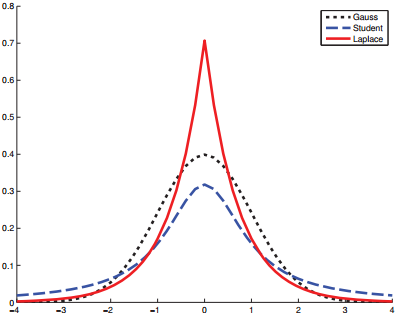
\includegraphics[scale=.70]{pdfs-for-NTL-a.png}} \\
\subfloat[]{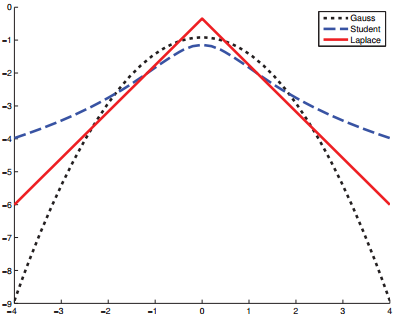
\includegraphics[scale=.70]{pdfs-for-NTL-b.png}}
\caption{(a) The pdf’s for a $\mathcal{N}(0,1)$, $\mathcal{T}(0,1,1)$ and $Lap(0,1/\sqrt{2})$. The mean is 0 and the variance is 1 for both the Gaussian and Laplace. The mean and variance of the Student is undefined when $\nu=1$.(b) Log of these pdf’s. Note that the Student distribution is not log-concave for any parameter value, unlike the Laplace distribution, which is always log-concave (and log-convex...) Nevertheless, both are unimodal.}
\label{fig:pdfs-for-NTL} 
\end{figure}

The variance is only defined if $\nu>2$. The mean is only defined if $\nu>1$.

As an illustration of the robustness of the Student distribution, consider Figure \ref{fig:robustness}. We see that the Gaussian is affected a lot, whereas the Student distribution hardly changes. This is because the Student has heavier tails, at least for small $\nu$(see Figure \ref{fig:pdfs-for-NTL}).

\begin{figure}[hbtp]
\centering
\subfloat[]{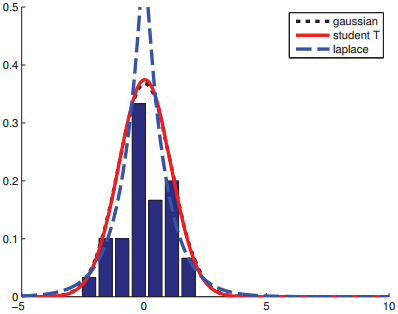
\includegraphics[scale=.70]{robustness-a.png}} \\
\subfloat[]{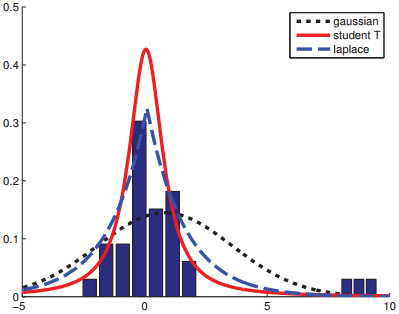
\includegraphics[scale=.70]{robustness-b.png}}
\caption{Illustration of the effect of outliers on fitting Gaussian, Student and Laplace distributions. (a) No outliers (the Gaussian and Student curves are on top of each other). (b) With outliers. We see that the Gaussian is more affected by outliers than the Student and Laplace distributions.}
\label{fig:robustness} 
\end{figure}

If $\nu=1$, this distribution is known as the \textbf{Cauchy} or \textbf{Lorentz} distribution. This is notable for having such heavy tails that the integral that defines the mean does not converge.

To ensure finite variance, we require $\nu>2$. It is common to use $\nu=4$, which gives good performance in a range of problems (Lange et al. 1989). For $\nu \gg 5$, the Student distribution rapidly approaches a Gaussian distribution and loses its robustness properties.


\subsection{The Laplace distribution}
\begin{table}
\caption{Summary of Laplace distribution.}
\centering
\begin{tabular}{cccccc}
\hline\noalign{\smallskip}
Written as & $f(x)$ & $\mathbb{E}[X]$ & mode & $\text{var}[X]$ \\
\noalign{\smallskip}\svhline\noalign{\smallskip}
$X \sim \text{Lap}(\mu,b)$ & $\dfrac{1}{2b}\exp\left(-\dfrac{|x-\mu|}{b}\right)$ & $\mu$ & $\mu$ & $2b^2$ \\
\noalign{\smallskip}\hline
\end{tabular}
\end{table}

Here $\mu$ is a location parameter and $b>0$ is a scale parameter. See Figure \ref{fig:pdfs-for-NTL} for a plot.

Its robustness to outliers is illustrated in Figure \ref{fig:robustness}. It also put mores probability density at 0 than the Gaussian. This property is a useful way to encourage sparsity in a model, as we will see in Section TODO.


\subsection{The gamma distribution}

\begin{table}
\caption{Summary of gamma distribution}
\centering
\begin{tabular}{ccccccc}
\hline\noalign{\smallskip}
Written as & $X$ & $f(x)$ & $\mathbb{E}[X]$ & mode & $\text{var}[X]$ \\
\noalign{\smallskip}\svhline\noalign{\smallskip}
$X \sim \text{Ga}(a,b)$ & $x \in \mathbb{R}^+$ & $\dfrac{b^a}{\Gamma(a)}x^{a-1}e^{-xb}$ & $\dfrac{a}{b}$ & $\dfrac{a-1}{b}$ & $\dfrac{a}{b^2}$ \\
\noalign{\smallskip}\hline
\end{tabular}
\end{table} 

Here $a>0$ is called the shape parameter and $b>0$ is called the rate parameter. See Figure \ref{fig:gamma-distribution} for some plots.

\begin{figure}[hbtp]
\centering
\subfloat[]{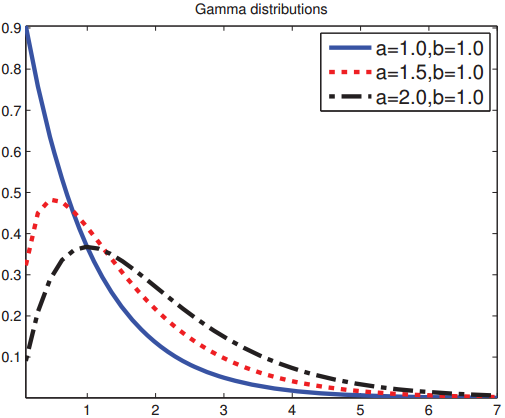
\includegraphics[scale=.50]{gamma-distribution-a.png}} \\
\subfloat[]{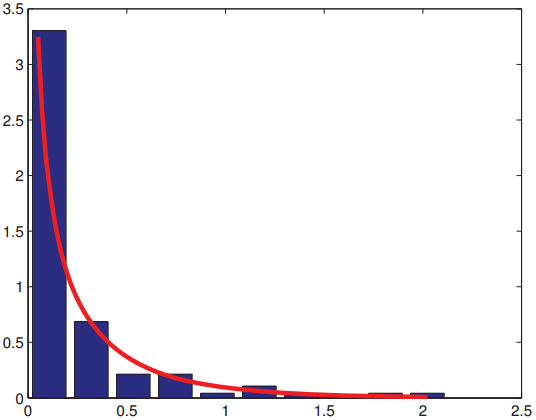
\includegraphics[scale=.50]{gamma-distribution-b.png}}
\caption{Some Ga$(a, b=1)$ distributions. If $a \leq 1$, the mode is at 0, otherwise it is $>0$.As we increase the rate $b$, we reduce the horizontal scale, thus squeezing everything leftwards and upwards. (b) An empirical pdf of some rainfall data, with a fitted Gamma distribution superimposed.}
\label{fig:gamma-distribution} 
\end{figure}


\subsection{The beta distribution}

\begin{table*}
\caption{Summary of Beta distribution}\label{tab:beta-distribution}
\centering
\begin{tabular}{ccccccc}
\hline\noalign{\smallskip}
Name & Written as & $X$ & $f(x)$ & $\mathbb{E}[X]$ & mode & $\text{var}[X]$ \\
\noalign{\smallskip}\svhline\noalign{\smallskip}
Beta distribution & $X \sim \text{Beta}(a,b)$ & $x \in [0,1]$ & $\dfrac{1}{B(a,b)}x^{a-1}(1-x)^{b-1}$ & $\dfrac{a}{a+b}$ & $\dfrac{a-1}{a+b-2}$ & $\dfrac{ab}{(a+b)^2(a+b+1)}$ \\
\noalign{\smallskip}\hline
\end{tabular}
\end{table*} 

Here $B(a, b)$is the beta function,
\begin{equation}
B(a,b) \triangleq \dfrac{\Gamma(a)\Gamma(b)}{\Gamma(a+b)}
\end{equation}

See Figure \ref{fig:beta-distribution} for plots of some beta distributions. We require  $a, b >0$ to ensure the distribution is integrable (i.e., to ensure $B(a, b)$ exists). If $a=b=1$, we get the uniform distirbution. If $a$ and $b$ are both less than 1, we get a bimodal distribution with “spikes” at 0 and 1; if $a$ and $b$ are both greater than 1, the distribution is unimodal.

\begin{figure}[hbtp]
\centering
    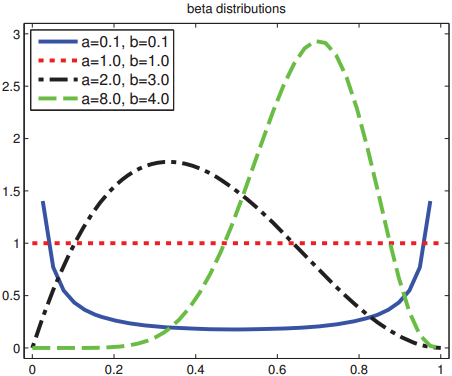
\includegraphics[scale=.60]{beta-distribution.png}
\caption{Some beta distributions.}
\label{fig:beta-distribution} 
\end{figure}


\subsection{Pareto distribution}

\begin{table*}
\caption{Summary of Pareto distribution}
\centering
\begin{tabular}{ccccccc}
\hline\noalign{\smallskip}
Name & Written as & $X$ & $f(x)$ & $\mathbb{E}[X]$ & mode & $\text{var}[X]$ \\
\noalign{\smallskip}\svhline\noalign{\smallskip}
Pareto distribution & $X \sim \text{Pareto}(k,m)$ & $x \geq m$ & $km^kx^{-(k+1)}\mathbb{I}(x \geq m)$ & $\dfrac{km}{k-1} \text{ if } k > 1$ & $m$ & $\dfrac{m^2k}{(k-1)^2(k-2)} \text{ if } k>2$ \\
\noalign{\smallskip}\hline
\end{tabular}
\end{table*} 

The \textbf{Pareto distribution} is used to model the distribution of quantities that exhibit \textbf{long tails}, also called \textbf{heavy tails}.

As $k \rightarrow \infty$, the distribution approaches $\delta(x-m)$. See Figure \ref{fig:Pareto-distribution}(a) for some plots. If we plot the distribution on a log-log scale, it forms a straight line, of the form $\log p(x)=a\log x+c$ for some constants $a$ and $c$. See Figure \ref{fig:Pareto-distribution}(b) for an illustration (this is known as a \textbf{power law}).

\begin{figure}[hbtp]
\centering
\subfloat[]{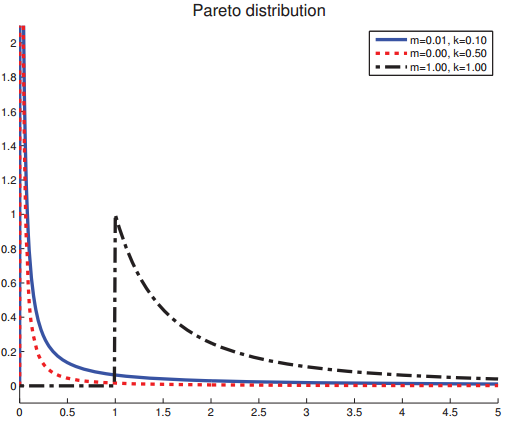
\includegraphics[scale=.50]{pareto-distribution-a.png}} \\
\subfloat[]{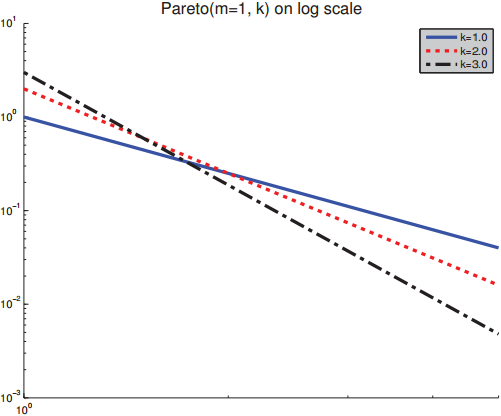
\includegraphics[scale=.50]{pareto-distribution-b.png}}
\caption{(a) The Pareto distribution Pareto$(x|m, k)$ for $m=1$. (b) The pdf on a log-log scale.}
\label{fig:Pareto-distribution} 
\end{figure}

\section{The Gaussian Distribution}
\label{sec:Gaussian distribution}
The Gaussian distributions,also known as the normal distributions,is a widely used model for the distribution of continuous variables.In the case of single variable $x$,the Gaussian is in the form
\begin{align}\label{eqn:univariate Gaussian distributions}
\mathcal{N}(x|\mu,\sigma^2)=\dfrac{1}{(2\pi\sigma^2)^{1/2}}\exp\{-\dfrac{1}{(2\sigma)^2}(x-\mu)^2 \}
\end{align}
where $\mu$ is the mean and $\sigma^2$ is the variance.For a $D$-dimensional vector $\vec{x}$,the multivariate Gaussian distribution takes the form
\begin{align}\label{eqn:multivariate Gaussian}
	\mathcal{N}(\vec{x}|\vec{\mu},\vec{\Sigma})
	=\dfrac{1}{(2\pi)^{D/2}}\dfrac{1}{\mid \vec{\Sigma}\mid^{1/2}}
	\exp\{-\dfrac{1}{2}(\vec{x}-\vec{\mu})^T\vec{\Sigma}^{-1}(\vec{x}-\vec{\mu}) \}
\end{align}
where $\vec{\mu}$ is a $D$-dimensional mean vector,$\vec{\Sigma}$ is a $D\times D$ covariance matrix,and $\mid\vec{\Sigma}\mid$ denotes the determinant of $\vec{\Sigma}$.

The Gaussian distribution arises in many different contexts and can be motivated from a variety of different perspectives,such as maximizing the entropy and the sum of multiple random variables.The \textbf{central limit theorem} tells us the latter.


\subsection{Conditional Gaussian distributions}
\subsection{Marginal Gaussian distributions}
\subsection{Baye's theorem for Gaussian variables}

\section{The exponential family}
\label{sec:exponential-family}

Before defining the exponential family, we mention several reasons why it is important:
\begin{itemize}
	\item{It can be shown that, under certain regularity conditions, the exponential family is the only family of distributions with finite-sized sufficient statistics, meaning that we can compress the data into a fixed-sized summary without loss of information. This is particularly useful for online learning, as we will see later.}
	\item{The exponential family is the only family of distributions for which conjugate priors exist, which simplifies the computation of the posterior (see Section \ref{sec:Bayes-for-the-exponential-family}).}
	\item{The exponential family can be shown to be the family of distributions that makes the least set of assumptions subject to some user-chosen constraints (see Section \ref{sec:Maximum-entropy-derivation-of-the-exponential-family}).}
	\item{The exponential family is at the core of generalized linear models, as discussed in Section \ref{sec:GLMs}.}
	\item{The exponential family is at the core of variational inference, as discussed in Section TODO.}
\end{itemize}


\subsection{Definition}
A pdf or pmf $p(\vec{x}|\vec{\theta})$,for $\vec{x} \in \mathbb{R}^m$ and $\vec{\theta} \in \mathbb{R}^D$, is said to be in the \textbf{exponential family} if it is of the form
\begin{align}
p(\vec{x}|\vec{\theta}) 
&= h(\vec{x})g(\vec{\theta})\exp\{\vec{\theta}^T\vec{\phi}(\vec{x})\} \\
&=\dfrac{1}{Z(\vec{\theta})}h(\vec{x})\exp[\vec{\theta}^T\phi(\vec{x})] \\
& = h(\vec{x})\exp[\vec{\theta}^T\phi(\vec{x})-A(\vec{\theta})] \label{eqn:exponential-family}
\end{align}
where
\begin{align}
Z(\vec{\theta}) & =\int h(\vec{x})\exp[\vec{\theta}^T\phi(\vec{x})]\mathrm{d}\vec{x} \\
A(\vec{\theta}) & =\log Z(\vec{\theta})
\end{align}

Here $\vec{\theta}$ are called the \textbf{natural parameters} or \textbf{canonical parameters}, $\phi(\vec{x}) \in \mathbb{R}^D$ is called a vector of \textbf{sufficient statistics}, $Z(\vec{\theta})$ is called the \textbf{partition function}, $A(\vec{\theta})$ is called the \textbf{log partition function} or \textbf{cumulant function}, and $h(\vec{x})$ is the a scaling constant, often 1. If $\phi(\vec{x})=\vec{x}$, we say it is a \textbf{natural exponential family}.

Equation \ref{eqn:exponential-family} can be generalized by writing
\begin{equation}
p(\vec{x}|\vec{\theta}) = h(\vec{x})\exp[\eta(\vec{\theta})^T\phi(\vec{x})-A(\eta(\vec{\theta}))]
\end{equation}
where $\eta$ is a function that maps the parameters $\vec{\theta}$ to the canonical parameters $\vec{\eta}=\eta(\vec{\theta})$.If $\mathrm{dim}(\vec{\theta})<\mathrm{dim}(\eta(\vec{\theta}))$, it is called a \textbf{curved exponential family}, which means we have more sufficient statistics than parameters. If $\eta(\vec{\theta})=\vec{\theta}$, the model is said to be in \textbf{canonical form}. We will assume models are in canonical form unless we state otherwise.

\subsection{Maximum likelihood and sufficient statistics}

\subsection{Conjugate priors}

\subsection{Noninformative prios}
In many cases,however,we may have little idea of what form the distribution should take.We may then seek a form of prior distribution,called a \textbf{noninformative prior},which is intended to have little influence on the posterior distribution as possible(Jeffries,1946;Box and Tao,1973;Bernardo and Smith,1994).

Suppose we have a distribution $p(x|\lambda)$ governed by a parameter $\lambda$,we might be tempted to propose a prior distribution $p(\lambda) = $const as a suitable prior.Improper priors are ones in which the domain $\lambda$ is unbounded and the prior distribution cannot be correctly normalized because the integral over $\lambda$ diverges.A second difficulty arises from the transformation behaviour of a probability density under a nonlinear change of variables.For example
\begin{equation}
p_\eta(\eta) = p_\lambda(\lambda) \left | \dfrac{d\lambda}{d\eta} \right | = p_\lambda(\eta^2)\eta\propto \eta
\end{equation}
so the density over $\eta$ will not be constant.

Here are two simple examples of noninformative priors(Berger,1985).
First of all,if a density takes the form
\begin{equation}
p(x|\mu) = f(x-\mu)
\end{equation}
then the parameter $\mu$ is known as a \textbf{location parameter}.This family of densities exhibits \textbf{translation invariance} because if we shift $x$ by a constant to give $\hat{x} = x+c$,then
\begin{equation}
p(\hat{x}|\hat{\mu}) = f(\hat{x}-\hat{\mu})
\end{equation}
where $\hat{\mu} = \mu +c$.

A second example,
\begin{equation}\label{eqn:density scale parameter}
p(x|\sigma) = \dfrac{1}{\sigma}f(\dfrac{x}{\sigma})
\end{equation}
where $\sigma>0$.Note that this will be a normalized density provided f(x) is correctly normalized.The parameter $\sigma$ is known as a \textbf{scale parameter},and the density exhibits \textbf{scale invariance}.

\subsection{Examples}


\subsubsection{Bernoulli}
The Bernoulli for $x \in \{0,1\}$ can be written in exponential family form as follows:
\begin{equation}\begin{split}
\mathrm{Ber}(x|\mu)& =\mu^x(1-\mu)^{1-x} \\
& =\exp[x\log\mu+(1-x)\log(1-\mu)]
\end{split}\end{equation}
where $\phi(x)=(\mathbb{I}(x=0),\mathbb{I}(x=1))$ and $\vec{\theta}=(\log\mu,\log(1-\mu))$. 

However, this representation is \textbf{over-complete} since $\vec{1}^T\phi(x)=\mathbb{I}(x=0)+\mathbb{I}(x=1)=1$. Consequently $\vec{\theta}$ is not uniquely identifiable. It is common to require that the representation be \textbf{minimal}, which means there is a unique $\theta$ associated with the distribution. In this case, we can just define
\begin{align}
\mathrm{Ber}(x|\mu) & =(1-\mu)\exp\left(x\log\dfrac{\mu}{1-\mu}\right) \\
\text{where } \phi(x) & =x, \theta=\log\dfrac{\mu}{1-\mu}, Z=\dfrac{1}{1-\mu}  \nonumber
\end{align}

We can recover the mean parameter $\mu$ from the canonical parameter using
\begin{equation}
\mu=\mathrm{sigm}(\theta)=\dfrac{1}{1+e^{-\theta}}
\end{equation}


\subsubsection{Multinoulli}
We can represent the multinoulli as a minimal exponential family as follows:
\begin{equation*}\begin{split}
& \mathrm{Cat}(\vec{x}|\vec{\mu}) = \prod\limits_{k=1}^K = \exp\left(\sum\limits_{k=1}^K x_k\log\mu_k\right) \\
& = \exp\left[\sum\limits_{k=1}^{K-1} x_k\log\mu_k+  (1-\sum\limits_{k=1}^{K-1} x_k)\log(1-\sum\limits_{k=1}^{K-1} \mu_k)\right] \\
& = \exp\left[\sum\limits_{k=1}^{K-1} x_k\log\dfrac{\mu_k}{1-\sum_{k=1}^{K-1} \mu_k} + \log(1-\sum\limits_{k=1}^{K-1} \mu_k) \right] \\
& = \exp\left[\sum\limits_{k=1}^{K-1} x_k\log\dfrac{\mu_k}{\mu_K}+\log\mu_K\right] \text{, where } \mu_K \triangleq 1-\sum\limits_{k=1}^{K-1} \mu_k
\end{split}\end{equation*}

We can write this in exponential family form as follows:
\begin{align}
\mathrm{Cat}(\vec{x}|\vec{\mu}) & = \exp[\vec{\theta}^T\phi(\vec{x})-A(\vec{\theta})] \\
\vec{\theta} & \triangleq (\log\dfrac{\mu_1}{\mu_K},\cdots,\log\dfrac{\mu_{K-1}}{\mu_K}) \\
\phi(\vec{x}) & \triangleq (x_1,\cdots,x_{K-1})
\end{align}

We can recover the mean parameters from the canonical parameters using
\begin{align}
\mu_k & = \dfrac{e^{\theta_k}}{1+\sum_{j=1}^{K-1} e^{\theta_j}} \\
\mu_K & = 1- \dfrac{\sum_{j=1}^{K-1} e^{\theta_j}}{1+\sum_{j=1}^{K-1} e^{\theta_j}}=\dfrac{1}{1+\sum_{j=1}^{K-1} e^{\theta_j}}
\end{align}
and hence
\begin{equation}
A(\vec{\theta]} = -\log\mu_K=\log(1+\sum\limits_{j=1}^{K-1} e^{\theta_j})
\end{equation}


\subsubsection{Univariate Gaussian}
The univariate Gaussian can be written in exponential family form as follows:
\begin{align}
\mathcal{N}(x|\mu,\sigma^2) & =\dfrac{1}{\sqrt{2\pi}\sigma}\exp\left[-\dfrac{1}{2\sigma^2}(x-\mu)^2\right] \nonumber \\
& = \dfrac{1}{\sqrt{2\pi}\sigma}\exp\left[-\dfrac{1}{2\sigma^2}x^2+\dfrac{\mu}{\sigma^2}x-\dfrac{1}{2\sigma^2}\mu^2\right] \nonumber \\
& = \dfrac{1}{Z(\vec{\theta})}\exp[\vec{\theta}^T\phi(x)]
\end{align}
where
\begin{align}
\vec{\theta} & = (\dfrac{\mu}{\sigma^2}, -\dfrac{1}{2\sigma^2}) \\
\phi(x) & =(x,x^2) \\
Z(\vec{\theta}) & =\sqrt{2\pi}\sigma\exp(\dfrac{\mu^2}{2\sigma^2})
\end{align}


\subsubsection{Non-examples}
Not all distributions of interest belong to the exponential family. For example, the uniform distribution,$X \sim U(a,b)$, does not, since the support of the distribution depends on the parameters. Also, the Student T distribution (Section TODO) does not belong, since it does not have the required form.


\subsection{Log partition function}
An important property of the exponential family is that derivatives of the log partition function can be used to generate \textbf{cumulants} of the sufficient statistics.\footnote{The first and second cumulants of a distribution are its mean $\mathbb{E}[X]$ and variance $\mathrm{var}[X]$, whereas the first and second moments are its mean $\mathbb{E}[X]$ and $\mathbb{E}[X^2]$.} For this reason, $A(\vec{\theta})$ is sometimes called a \textbf{cumulant function}. We will prove this for a 1-parameter distribution; this can be generalized to a $K$-parameter distribution in a straightforward way. For the first derivative we have

For the second derivative we have
\begin{align}
\dfrac{\mathrm{d} A}{\mathrm{d} \theta} & = \dfrac{\mathrm{d}}{\mathrm{d} \theta}\left\{\log\int\exp\left[\theta\phi(x)\right]h(x)\mathrm{d}x\right\} \nonumber \\
& = \dfrac{\frac{\mathrm{d}}{\mathrm{d} \theta}\int\exp\left[\theta\phi(x)\right]h(x)\mathrm{d}x}{\int\exp\left[\theta\phi(x)\right]h(x)\mathrm{d}x} \nonumber \\
& = \dfrac{\int\phi(x)exp\left[\theta\phi(x)\right]h(x)\mathrm{d}x}{\exp(A(\theta))} \nonumber \\
& = \int \phi(x)\exp\left[\theta\phi(x)-A(\theta)\right]h(x)\mathrm{d}x \nonumber \\
& = \int \phi(x)p(x)\mathrm{d}x=\mathbb{E}[\phi(x)]
\end{align}

For the second derivative we have
\begin{align}
\dfrac{\mathrm{d}^2 A}{\mathrm{d} \theta^2} & = \int \phi(x)\exp\left[\theta\phi(x)-A(\theta)\right]h(x)\left[\phi(x)-A'(\theta)\right]\mathrm{d}x \nonumber \\
& = \int \phi(x)p(x)\left[\phi(x)-A'(\theta)\right]\mathrm{d}x \nonumber \\
& = \int \phi^2(x)p(x)\mathrm{d}x-A'(\theta)\int \phi(x)p(x)\mathrm{d}x \nonumber \\
& = \mathbb{E}[\phi^2(x)]-\mathbb{E}[\phi(x)]^2=\mathrm{var}[\phi(x)]
\end{align}

In the multivariate case, we have that
\begin{equation}
\dfrac{\partial^2 A}{\partial \theta_i \partial \theta_j}=\mathbb{E}[\phi_i(x)\phi_j(x)]-\mathbb{E}[\phi_i(x)]\mathbb{E}[\phi_j(x)]
\end{equation}
and hence
\begin{equation}
\nabla^2A(\vec{\theta}) = \mathrm{cov}[\phi(\vec{x})]
\end{equation}

Since the covariance is positive definite, we see that $A(\vec{\theta})$ is a convex function (see Section \ref{sec:Convexity}).


\subsection{MLE for the exponential family}
The likelihood of an exponential family model has the form
\begin{equation}
p(\mathcal{D}|\vec{\theta})=\left[\prod\limits_{i=1}^N h(\vec{x}_i)\right]g(\vec{\theta})^N\exp\left[\vec{\theta}^T\left(\sum\limits_{i=1}^N \phi(\vec{x}_i)\right)\right]
\end{equation}

We see that the sufficient statistics are $N$ and
\begin{equation}
\phi(\mathcal{D})=\sum\limits_{i=1}^N \phi(\vec{x}_i)=(\sum\limits_{i=1}^N \phi_1(\vec{x}_i),\cdots,\sum\limits_{i=1}^N \phi_K(\vec{x}_i))
\end{equation}

The \textbf{Pitman-Koopman-Darmois theorem} states that, under certain regularity conditions, the exponential family is the only family of distributions with finite sufficient statistics. (Here, finite means of a size independent of the size of the data set.)

One of the conditions required in this theorem is that the support of the distribution not be dependent on the parameter.


\subsection{Bayes for the exponential family}
\label{sec:Bayes-for-the-exponential-family}
TODO


\subsubsection{Likelihood}



\subsection{Maximum entropy derivation of the exponential family *}
\label{sec:Maximum-entropy-derivation-of-the-exponential-family}


\section{Nonparametric Methods}
\subsection{Kernel density estimators}
\subsection{Nearest-neighbour methods}


\section{Joint probability distributions}
Given a \textbf{multivariate random variable} or \textbf{random vector} \footnote{\url{http://en.wikipedia.org/wiki/Multivariate_random_variable}} $X \in \mathbb{R}^D$, the \textbf{joint probability distribution}\footnote{\url{http://en.wikipedia.org/wiki/Joint_probability_distribution}} is a probability distribution that gives the probability that each of $X_1, X_2, \cdots,X_D$ falls in any particular range or discrete set of values specified for that variable. In the case of only two random variables, this is called a \textbf{bivariate distribution}, but the concept generalizes to any number of random variables, giving a \textbf{multivariate distribution}.

The joint probability distribution can be expressed either in terms of a \textbf{joint cumulative distribution function} or in terms of a \textbf{joint probability density function} (in the case of continuous variables) or \textbf{joint probability mass function} (in the case of discrete variables). 


\subsection{Covariance and correlation}
\begin{definition}
The \textbf{covariance} between two rv’s $X$ and $Y$ measures the degree to which $X$ and $Y$ are (linearly) related. Covariance is defined as
\begin{equation}
\begin{split}
\mathrm{cov}[X,Y] & \triangleq \mathbb{E}\left[(X-\mathbb{E}[X])(Y-\mathbb{E}[Y])\right] \\
         & =\mathbb{E}[XY]-\mathbb{E}[X]\mathbb{E}[Y]
\end{split}
\end{equation}
\end{definition}

\begin{definition}
If $X$ is a $D$-dimensional random vector, its \textbf{covariance matrix} is defined to be the following symmetric, positive definite matrix:
\begin{align}
\mathrm{cov}[\vec{x}] & \triangleq \mathbb{E}\left[(\vec{x}-\mathbb{E}[\vec{x}])(\vec{x}-\mathbb{E}[\vec{x}])^T\right] \\
       &  = \left( \begin{array}{cccc}
           \text{var}[\vec{x_1}] & \text{Cov}[\vec{x_1},\vec{x_2}] & \cdots & \text{Cov}[\vec{x_1},\vec{x_D}] \\
           \text{Cov}[\vec{x_2},\vec{x_1}] & \text{var}[x_2] & \cdots & \text{Cov}[\vec{x_2},\vec{x_D}] \\
		   \vdots & \vdots & \ddots & \vdots \\
           \text{Cov}[\vec{x_D},\vec{x_1}] & \text{Cov}[\vec{x_D},\vec{x_2}] & \cdots & \text{var}[\vec{x_D}] \end{array} \right)
\end{align}
\end{definition}
For 

\begin{definition}
The (Pearson) \textbf{correlation coefficient} between $X$ and $Y$ is defined as
\begin{equation}
\text{corr}[X,Y] \triangleq \dfrac{\text{Cov}[X,Y]}{\sqrt{\text{var}[X],\text{var}[Y]}}
\end{equation}
\end{definition}

A \textbf{correlation matrix} has the form
\begin{equation}
\mathbf{R} \triangleq \left( \begin{array}{cccc}
           \text{corr}[X_1,X_1] & \text{corr}[X_1,X_2] & \cdots & \text{corr}[X_1,X_D] \\
           \text{corr}[X_2,X_1] & \text{corr}[X_2,X_2] & \cdots & \text{corr}[X_2,X_D] \\
		   \vdots & \vdots & \ddots & \vdots \\
           \text{corr}[X_D,X_1] & \text{corr}[X_D,X_2] & \cdots & \text{corr}[X_D,X_D] \end{array} \right)
\end{equation}

The correlation coefficient can viewed as a degree of linearity between $X$ and $Y$, see Figure \ref{fig:Correlation-examples}.
\begin{figure*}[hbtp]
\centering
    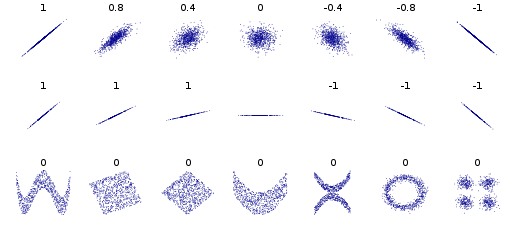
\includegraphics[scale=.80]{Correlation-examples.png}
\caption{Several sets of $(x, y)$ points, with the Pearson correlation coefficient of $x$ and $y$ for each set. Note that the correlation reflects the noisiness and direction of a linear relationship (top row), but not the slope of that relationship (middle), nor many aspects of nonlinear relationships (bottom). N.B.: the figure in the center has a slope of 0 but in that case the correlation coefficient is undefined because the variance of $Y$ is zero.Source:\url{http://en.wikipedia.org/wiki/Correlation}}
\label{fig:Correlation-examples} 
\end{figure*}

\textbf{Uncorrelated does not imply independent}. For example, let $X \sim U(-1,1)$ and $Y =X^2$. Clearly $Y$ is dependent on $X$(in fact, $Y$ is uniquely determined by $X$), yet one can show that corr$[X, Y]=0$. Some striking examples of this fact are shown in Figure \ref{fig:Correlation-examples}. This shows several data sets where there is clear dependence between $X$ and $Y$, and yet the correlation coefficient is 0. A more general measure of dependence between random variables is mutual information, see Section TODO.


\subsection{Multivariate Gaussian distribution}
\label{sec:MVN}
The \textbf{multivariate Gaussian} or \textbf{multivariate normal}(MVN) is the most widely used joint probability density function for continuous variables. We discuss MVNs in detail in Chapter 4; here we just give some definitions and plots.

The pdf of the MVN in $D$ dimensions is defined by the following:
\begin{equation}
\mathcal{N}(\vec{x}|\vec{\mu},\Sigma) \triangleq \dfrac{1}{(2\pi)^{D/2}|\Sigma|^{1/2}}\exp\left[-\dfrac{1}{2}(\vec{x}-\vec{\mu})^T\Sigma^{-1}(\vec{x}-\vec{\mu})\right]
\end{equation}
where $\vec{\mu}=\mathbb{E}[X] \in \mathbb{R}^D$ is the mean vector, and $\Sigma=\text{Cov}[X]$ is the $D \times D$ covariance matrix. The normalization constant $(2\pi)^{D/2}|\Sigma|^{1/2}$ just ensures that the pdf integrates to 1.

Figure \ref{fig:2d-Gaussions} plots some MVN densities in 2d for three different kinds of covariance matrices. A full covariance matrix has A $D(D+1)/2$ parameters (we divide by 2 since $\Sigma$ is symmetric). A diagonal covariance matrix has $D$ parameters, and has 0s in the off-diagonal terms. A spherical or isotropic covariance,$\Sigma=\sigma^2\vec{I}_D$, has one free parameter.

\begin{figure}[hbtp]
\centering
\subfloat[]{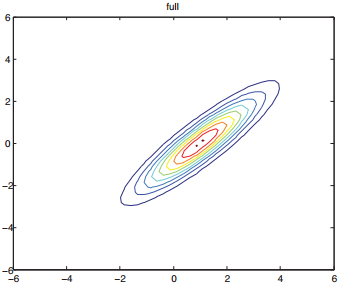
\includegraphics[scale=.60]{2d-Gaussions-a.png}} \\
\subfloat[]{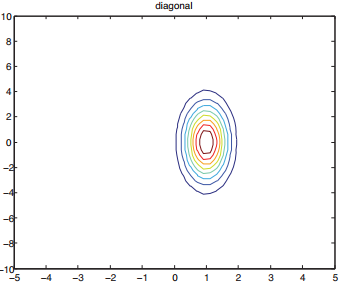
\includegraphics[scale=.60]{2d-Gaussions-b.png}} \\
\subfloat[]{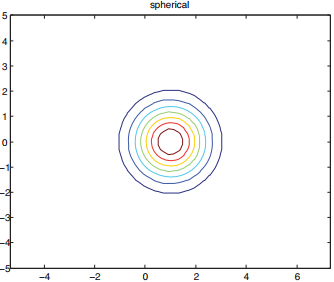
\includegraphics[scale=.60]{2d-Gaussions-c.png}} \\
\subfloat[]{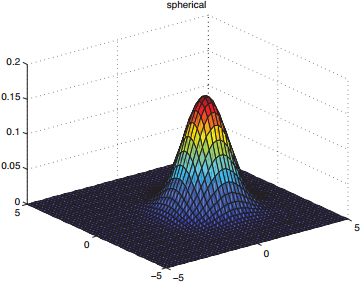
\includegraphics[scale=.60]{2d-Gaussions-d.png}}
\caption{We show the level sets for 2d Gaussians. (a) A full covariance matrix has elliptical contours.(b) A diagonal covariance matrix is an axis aligned ellipse. (c) A spherical covariance matrix has a circular shape. (d) Surface plot for the spherical Gaussian in (c).}
\label{fig:2d-Gaussions} 
\end{figure}


\subsection{Multivariate Student's t-distribution}
A more robust alternative to the MVN is the multivariate Student's t-distribution, whose pdf is given by
\begin{align}
& \mathcal{T}(x|\vec{\mu},\Sigma,\nu) \nonumber \\
& \triangleq \dfrac{\Gamma(\frac{\nu+D}{2})}{\Gamma(\frac{\nu}{2})}\dfrac{|\Sigma|^{-\frac{1}{2}}}{\left(\nu\pi\right)^{\frac{D}{2}}}\left[1+\dfrac{1}{\nu}\left(\vec{x}-\vec{\mu}\right)^T\Sigma^{-1}\left(\vec{x}-\vec{\mu}\right)\right]^{-\frac{\nu+D}{2}} \\
&= \dfrac{\Gamma(\frac{\nu+D}{2})}{\Gamma(\frac{\nu}{2})}\dfrac{|\Sigma|^{-\frac{1}{2}}}{\left(\nu\pi\right)^{\frac{D}{2}}}\left[1+\left(\vec{x}-\vec{\mu}\right)^T\vec{V}^{-1}\left(\vec{x}-\vec{\mu}\right)\right]^{-\frac{\nu+D}{2}}
\end{align}
where $\Sigma$ is called the scale matrix (since it is not exactly the covariance matrix) and $\vec{V}=\nu\Sigma$. This has fatter tails than a Gaussian. The smaller $\nu$ is, the fatter the tails. As $\nu \rightarrow \infty$, the distribution tends towards a Gaussian. The distribution has the following properties
\begin{equation}
\text{mean}=\vec{\mu} \text{ , mode}=\vec{\mu} \text{ , Cov}= \dfrac{\nu}{\nu-2}\Sigma
\end{equation}


\subsection{Dirichlet distribution}
A multivariate generalization of the beta distribution is the \textbf{Dirichlet distribution}, which has
support over the probability simplex, defined by
\begin{equation}
S_K=\left\{\vec{x}:0 \leq x_k \leq 1,\sum\limits_{k=1}^K x_k=1\right\}
\end{equation}

The pdf is defined as follows:
\begin{equation}
\text{Dir}(\vec{x}|\vec{\alpha}) \triangleq \dfrac{1}{B(\vec{\alpha})}\prod\limits_{k=1}^K x_k^{\alpha_k-1}\mathbb{I}(\vec{x} \in S_K)
\end{equation}
where $B(\alpha_1,\alpha_2,\cdots,\alpha_K)$ is the natural generalization of the beta function to $K$ variables:
\begin{equation}
B(\alpha) \triangleq \dfrac{\prod_{k=1}^K \Gamma(\alpha_k)}{\Gamma(\alpha_0)} \text{ where } \alpha_0 \triangleq \sum_{k=1}^K \alpha_k
\end{equation}

Figure \ref{fig:3d-Dirichlet} shows some plots of the Dirichlet when $K=3$, and Figure \ref{fig:5d-Dirichlet} for some sampled probability vectors. We see that $\alpha_0$ controls the strength of the distribution (how peaked it is), and theαkcontrol where the peak occurs. For example, Dir$(1,1,1)$ is a uniform distribution, Dir$(2,2,2)$ is a broad distribution centered at $(1/3,1/3,1/3)$, and Dir$(20,20,20)$ is a narrow distribution centered at $(1/3,1/3,1/3)$.If $\alpha_k < 1$ for all $k$, we get “spikes” at the corner of the simplex.

\begin{figure}[hbtp]
\centering
\subfloat[]{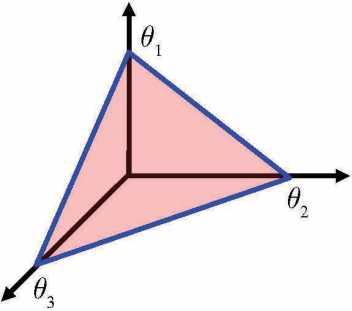
\includegraphics[scale=.50]{3d-Dirichlet-a.png}} \\
\subfloat[]{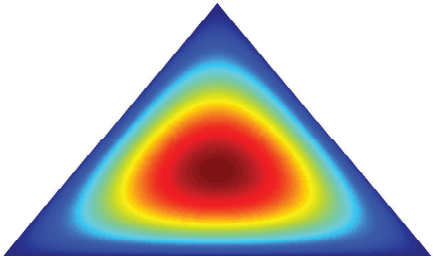
\includegraphics[scale=.60]{3d-Dirichlet-b.png}} \\
\subfloat[]{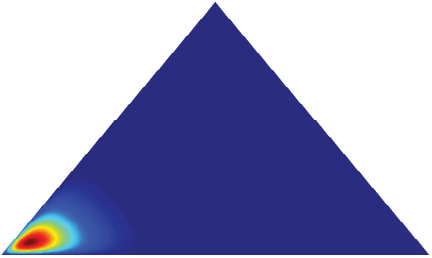
\includegraphics[scale=.60]{3d-Dirichlet-c.png}} \\
\subfloat[]{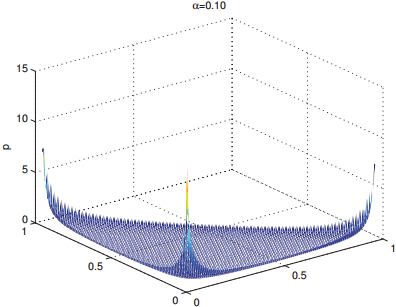
\includegraphics[scale=.60]{3d-Dirichlet-d.png}}
\caption{(a) The Dirichlet distribution when $K=3$ defines a distribution over the simplex, which can be represented by the triangular surface. Points on this surface satisfy $0 \leq \theta_k \leq 1$ and $\sum_{k=1}^K \theta_k=1$. (b) Plot of the Dirichlet density when $\vec{\alpha}=(2,2,2)$. (c) $\vec{\alpha}=(20,2,2)$.}
\label{fig:3d-Dirichlet} 
\end{figure}

\begin{figure}[hbtp]
\centering
\subfloat[$\vec{\alpha}=(0.1,\cdots,0.1)$. This results in very sparse distributions, with many 0s.]{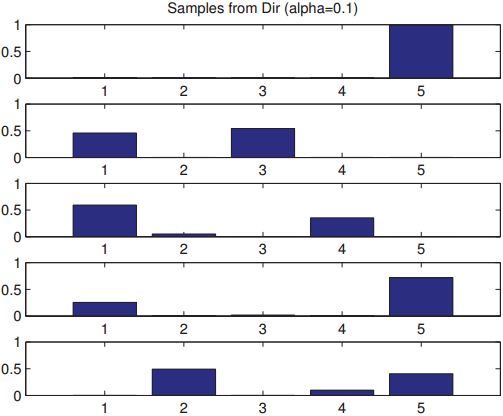
\includegraphics[scale=.50]{5d-Dirichlet-a.png}} \\
\subfloat[$\vec{\alpha}=(1,\cdots,1)$. This results in more uniform (and dense) distributions.]{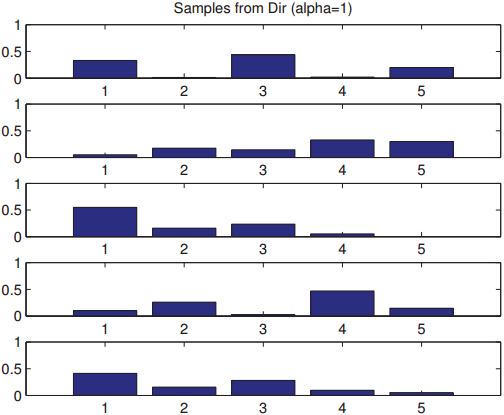
\includegraphics[scale=.50]{5d-Dirichlet-b.png}}
\caption{Samples from a 5-dimensional symmetric Dirichlet distribution for different parameter values.} 
\label{fig:5d-Dirichlet} 
\end{figure}

For future reference, the distribution has these properties
\begin{equation}\label{eqn:Dirichlet-properties}
\mathbb{E}(x_k)=\dfrac{\alpha_k}{\alpha_0} \text{, mode}[x_k]=\dfrac{\alpha_k-1}{\alpha_0-K} \text{, var}[x_k]=\dfrac{\alpha_k(\alpha_0-\alpha_k)}{\alpha_0^2(\alpha_0+1)}
\end{equation}


\section{Transformations of random variables}
If $\vec{x} \sim P()$ is some random variable, and $\vec{y}=f(\vec{x})$, what is the distribution of $Y$? This is the question we address in this section.


\subsection{Linear transformations}
Suppose $g()$ is a linear function: 
\begin{equation}
g(\vec{x})=A\vec{x}+b
\end{equation}

First, for the mean, we have
\begin{equation}
\mathbb{E}[\vec{y}]=\mathbb{E}[A\vec{x}+b]=A\mathbb{E}[\vec{x}]+b
\end{equation}
this is called the \textbf{linearity of expectation}.

For the covariance, we have
\begin{equation}
\text{Cov}[\vec{y}]=\text{Cov}[A\vec{x}+b]=A\Sigma A^T
\end{equation}


\subsection{General transformations}
\label{sec:General-transformations}
If $X$ is a discrete rv, we can derive the pmf for $y$ by simply summing up the probability mass for all the $x$’s such that $f(x)=y$:
\begin{equation}\label{eqn:transformation-discrete}
p_Y(y)=\sum\limits_{x:g(x)=y}p_X(x)
\end{equation}

If $X$ is continuous, we cannot use Equation \ref{eqn:transformation-discrete} since $p_X(x)$ is a density, not a pmf, and we cannot sum up densities. Instead, we work with cdf’s, and write
\begin{equation}
F_Y(y)=P(Y \leq y)=P(g(X) \leq y)=\int\limits_{g(X) \leq y} f_X(x)\mathrm{d}x
\end{equation}

We can derive the pdf of $Y$ by differentiating the cdf:
\begin{equation}\label{eqn:General-transformations}
f_Y(y)=f_X(x)|\dfrac{dx}{dy}|
\end{equation}

This is called \textbf{change of variables} formula. We leave the proof of this as an exercise. 

For example, suppose $X \sim U(−1,1)$, and $Y=X^2$. Then $p_Y(y)=\dfrac{1}{2}y^{-\frac{1}{2}}$.


\subsubsection{Multivariate change of variables *}
Let $f$ be a function $f:\mathbb{R}^n \rightarrow \mathbb{R}^n$, and let $\vec{y}=f(\vec{x})$. Then its Jacobian matrix $\vec{J}$ is given by
\begin{equation}
\vec{J}_{\vec{x} \rightarrow \vec{y}} \triangleq \frac{\partial \vec{y}}{\partial \vec{x}} \triangleq \left(\begin{array}{ccc}
\frac{\partial y_1}{\partial x_1} & \cdots & \frac{\partial y_1}{\partial x_n} \\
\vdots & \vdots & \vdots \\
\frac{\partial y_n}{\partial x_1} & \cdots & \frac{\partial y_n}{\partial x_n}
\end{array}\right)
\end{equation}
$|\mathrm{det}(\vec{J})|$ measures how much a unit cube changes in volume when we apply $f$.

If $f$ is an invertible mapping, we can define the pdf of the transformed variables using the Jacobian of the inverse mapping $\vec{y} \rightarrow \vec{x}$:
\begin{equation}\label{eqn:Multivariate-transformation}
p_y(\vec{y})=p_x(\vec{x})|\mathrm{det}(\frac{\partial \vec{x}}{\partial \vec{y}})|=p_x(\vec{x})|\mathrm{det}(\vec{J}_{\vec{y} \rightarrow \vec{x}})|
\end{equation}


\subsection{Central limit theorem}
Given $N$ random variables $X_1,X_2,\cdots,X_N$, each variable is \textbf{independent and identically distributed}\footnote{\url{http://en.wikipedia.org/wiki/Independent_identically_distributed}}(\textbf{iid} for short), and each has the same mean $\mu$ and variance $\sigma^2$, then
\begin{equation}
\dfrac{\sum\limits_{i=1}^n X_i-N\mu}{\sqrt{N}\sigma} \sim \mathcal{N}(0,1)
\end{equation}
this can also be written as
\begin{equation}
\dfrac{\bar{X}-\mu}{\sigma/\sqrt{N}} \sim \mathcal{N}(0,1) \quad \text{, where } \bar{X} \triangleq \dfrac{1}{N}\sum\limits_{i=1}^n X_i
\end{equation}


\section{Monte Carlo approximation}
\label{sec:Monte-Carlo-approximation}
In general, computing the distribution of a function of an rv using the change of variables formula can be difficult. One simple but powerful alternative is as follows. First we generate $S$ samples from the distribution, call them $x_1,\cdots,x_S$. (There are many ways to generate such samples; one popular method, for high dimensional distributions, is called Markov chain Monte Carlo or MCMC; this will be explained in Chapter TODO.) Given the samples, we can approximate the distribution of $f(X)$ by using the empirical distribution of $\left\{f(x_s)\right\}_{s=1}^S$. This is called a \textbf{Monte Carlo approximation}\footnote{\url{http://en.wikipedia.org/wiki/Monte_Carlo_method}}, named after a city in Europe known for its plush gambling casinos.

We can use Monte Carlo to approximate the expected value of any function of a random variable. We simply draw samples, and then compute the arithmetic mean of the function applied to the samples. This can be written as follows:
\begin{equation}
\mathbb{E}[g(X)]=\int g(x)p(x)\mathrm{d}x \approx \dfrac{1}{S}\sum\limits_{s=1}^S f(x_s)
\end{equation}
where $x_s \sim p(X)$.

This is called \textbf{Monte Carlo integration}\footnote{\url{http://en.wikipedia.org/wiki/Monte_Carlo_integration}}, and has the advantage over numerical integration (which is based on evaluating the function at a fixed grid of points) that the function is only evaluated in places where there is non-negligible probability.


\section{Information theory}

\subsection{Entropy}
\label{sec:Entropy}
The entropy of a random variable $X$ with distribution $p$, denoted by $\mathbb{H}(X)$ or sometimes $\mathbb{H}(p)$, is a measure of its uncertainty. In particular, for a discrete variable with $K$ states, it is defined by
\begin{equation}
\mathbb{H}(X) \triangleq -\sum\limits_{k=1}^{K}{p(X=k)\log_2p(X=k)}
\end{equation}

Usually we use log base 2, in which case the units are called \textbf{bits}(short for binary digits). If we use log base $e$ , the units are called \textbf{nats}. 

The discrete distribution with maximum entropy is the uniform distribution (see Section XXX for a proof). Hence for a K-ary random variable, the entropy is maximized if $p(x = k)=1/K$; in this case, $\mathbb{H}(X)=\log_2K$. 

Conversely, the distribution with minimum entropy (which is zero) is any \textbf{delta-function} that puts all its mass on one state. Such a distribution has no uncertainty.


\subsection{KL divergence}
One way to measure the dissimilarity of two probability distributions, $p$ and $q$ , is known as the \textbf{Kullback-Leibler divergence}(\textbf{KL divergence})or \textbf{relative entropy}. This is defined as follows:
\begin{equation}
\mathbb{KL}(P||Q) \triangleq 
\sum\limits_{x}{p(x)\log_2\dfrac{p(x)}{q(x)}}
\end{equation}
where the sum gets replaced by an integral for pdfs\footnote{The KL divergence is not a distance, since it is asymmetric. One symmetric version of the KL divergence is the \textbf{Jensen-Shannon divergence}, defined as $JS(p_1,p_2)=0.5\mathbb{KL}(p_1||q)+0.5\mathbb{KL}(p_2||q)$,where $q=0.5p_1+0.5p_2$}. The KL divergence is only defined if P and Q both sum to 1 and if $q(x)=0$ implies $p(x)=0$ for all $x$(absolute continuity). If the quantity  $0\ln0$ appears in the formula, it is interpreted as zero because $\lim\limits_{x \to 0}x\ln x$. We can rewrite this as
\begin{equation}\begin{split}
\mathbb{KL}(p||q) & \triangleq \sum\limits_{x}{p(x)\log_2p(x)}-\sum\limits_{k=1}^{K}{p(x)\log_2q(x)} \\
    & =\mathbb{H}(p)-\mathbb{H}(p,q)
\end{split}\end{equation}
where $\mathbb{H}(p,q)$ is called the \textbf{cross entropy},
\begin{equation}\label{eqn:cross-entropy}
\mathbb{H}(p,q)=\sum\limits_{x}{p(x)\log_2q(x)}
\end{equation}

One can show (Cover and Thomas 2006) that the cross entropy is the average number of bits needed to encode data coming from a source with distribution $p$ when we use model $q$ to define our codebook. Hence the “regular” entropy $\mathbb{H}(p)=\mathbb{H}(p,p)$, defined in section \S \ref{sec:Entropy},is the expected number of bits if we use the true model, so the KL divergence is the diference between these. In other words, the KL divergence is the average number of \emph{extra} bits needed to encode the data, due to the fact that we used distribution $q$ to encode the data instead of the true distribution $p$.

The “extra number of bits” interpretation should make it clear that $\mathbb{KL}(p||q) \geq 0$, and that the KL is only equal to zero if $q = p$. We now give a proof of this important result.

\begin{theorem}
(\textbf{Information inequality}) $\mathbb{KL}(p||q) \geq 0 \text{ with equality iff } p=q$.
\end{theorem}

One important consequence of this result is that \emph{the discrete distribution with the maximum
entropy is the uniform distribution}.


\subsection{Mutual information}
\label{sec:Mutual-information}
\begin{definition}
\textbf{Mutual information} or \textbf{MI}, is defined as follows:
\begin{equation}\begin{split}
\mathbb{I}(X;Y) & \triangleq \mathbb{KL}(P(X,Y)||P(X)P(X)) \\
    & =\sum\limits_x\sum\limits_yp(x,y)\log\dfrac{p(x,y)}{p(x)p(y)}
\end{split}\end{equation}
We have $\mathbb{I}(X;Y) \geq 0$ with equality if $P(X,Y)=P(X)P(Y)$. That is, the MI is zero if the variables are independent.
\end{definition}

To gain insight into the meaning of MI, it helps to re-express it in terms of joint and conditional entropies. One can show that the above expression is equivalent to the following:
\begin{eqnarray}
\mathbb{I}(X;Y)&=&\mathbb{H}(X)-\mathbb{H}(X|Y)\\
               &=&\mathbb{H}(Y)-\mathbb{H}(Y|X)\\
               &=&\mathbb{H}(X)+\mathbb{H}(Y)-\mathbb{H}(X,Y)\\
               &=&\mathbb{H}(X,Y)-\mathbb{H}(X|Y)-\mathbb{H}(Y|X)
\end{eqnarray}
where $\mathbb{H}(X)$ and $\mathbb{H}(Y)$ are the \textbf{marginal entropies}, $\mathbb{H}(X|Y)$ and $\mathbb{H}(Y|X)$ are the \textbf{conditional entropies}, and $\mathbb{H}(X,Y)$ is the \textbf{joint entropy} of $X$ and $Y$, see Fig. \ref{fig:mi}\footnote{\url{http://en.wikipedia.org/wiki/Mutual_information}}.

\begin{figure}[hbtp]
\centering
    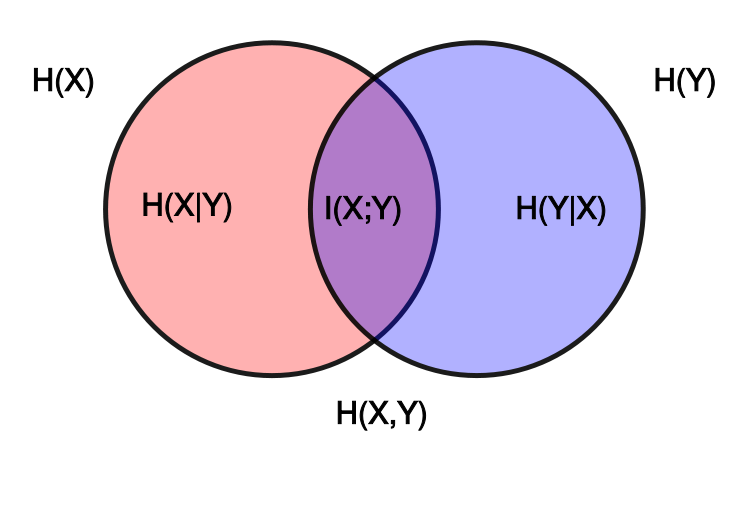
\includegraphics[scale=.25]{mutual-information.png}
\caption{Individual $\mathbb{H}(X),\mathbb{H}(Y)$, joint $\mathbb{H}(X,Y)$, and conditional entropies for a pair of correlated subsystems $X,Y$ with mutual information $\mathbb{I}(X;Y)$.}
\label{fig:mi} 
\end{figure}

Intuitively, we can interpret the MI between $X$ and $Y$ as the reduction in uncertainty about $X$ after observing $Y$, or, by symmetry, the reduction in uncertainty about $Y$ after observing $X$.

A quantity which is closely related to MI is the \textbf{pointwise mutual information} or \textbf{PMI}. For two events (not random variables) $x$ and $y$, this is defined as
\begin{equation}
PMI(x,y) \triangleq \log\dfrac{p(x,y)}{p(x)p(y)}=\log\dfrac{p(x|y)}{p(x)}=\log\dfrac{p(y|x)}{p(y)}
\end{equation}

This measures the discrepancy between these events occuring together compared to what would be expected by chance. Clearly the MI of $X$ and $Y$ is just the expected value of the PMI. Interestingly, we can rewrite the PMI as follows:
\begin{equation}
PMI(x,y)=\log\dfrac{p(x|y)}{p(x)}=\log\dfrac{p(y|x)}{p(y)}
\end{equation}

This is the amount we learn from updating the prior $p(x)$ into the posterior $p(x|y)$ , or equivalently, updating the prior $p(y)$ into the posterior $p(y |x)$ .
\chapter{Generative models for discrete data}

\section{Generative classifier}
\begin{equation}\label{eqn:Generative-classifier}
p(y=c|\vec{x},\vec{\theta})=\dfrac{p(y=c|\vec{\theta})p(\vec{x}|y=c,\vec{\theta})}{\sum_{c'}{p(y=c'|\vec{\theta})p(\vec{x}|y=c',\vec{\theta})}}
\end{equation}

This is called a \textbf{generative classifier}, since it specifies how to generate the data using the \textbf{class conditional density} $p(\vec{x}|y=c)$ and the class prior $p(y=c)$. An alternative approach is to directly fit the class posterior, $p(y=c|\vec{x})$ ;this is known as a \textbf{discriminative classifier}. 


\section{Bayesian concept learning}
Psychological research has shown that people can learn concepts from positive examples alone (Xu and Tenenbaum 2007).

We can think of learning the meaning of a word as equivalent to \textbf{concept learning}, which in turn is equivalent to binary classification. To see this, define $f(\vec{x})=1$ if xis an example of the concept $C$, and $f(\vec{x})=0$ otherwise. Then the goal is to learn the indicator function $f$, which just defines which elements are in the set $C$.


\subsection{Likelihood}
\begin{equation}
p(\mathcal{D}|h) \triangleq \left(\dfrac{1}{\text{size}(h)}\right)^N=\left(\dfrac{1}{|h|}\right)^N
\end{equation}

This crucial equation embodies what Tenenbaum calls the \textbf{size principle}, which means the model favours the simplest (smallest) hypothesis consistent with the data. This is more commonly known as \textbf{Occam’s razor}\footnote{\url{http://en.wikipedia.org/wiki/Occam\%27s_razor}}.


\subsection{Prior}
The prior is decided by human, not machines, so it is subjective. The subjectivity of the prior is controversial. For example, that a child and a math professor will reach different answers. In fact, they presumably not only have different priors, but also different hypothesis spaces. However, we can finesse that by defining the hypothesis space of the child and the math professor to be the same, and then setting the child’s prior weight to be zero on certain “advanced” concepts. Thus there is no sharp distinction between the prior and the hypothesis space.

However, the prior is the mechanism by which background knowledge can be brought to bear on a problem. Without this, rapid learning (i.e., from small samples sizes) is impossible.


\subsection{Posterior}
The posterior is simply the likelihood times the prior, normalized.
\begin{equation}
p(h|\mathcal{D}) \triangleq \dfrac{p(\mathcal{D}|h)p(h)}{\sum_{h' \in \mathcal{H}}p(\mathcal{D}|h')p(h')}=\dfrac{\mathbb{I}(\mathcal{D} \in h)p(h)}{\sum_{h' \in \mathcal{H}}\mathbb{I}(\mathcal{D} \in h')p(h')}
\end{equation}
where $\mathbb{I}(\mathcal{D} \in h)p(h)$ is 1 \textbf{iff}(iff and only if) all the data are in the extension of the hypothesis $h$.

In general, when we have enough data, the posterior $p(h|\mathcal{D})$ becomes peaked on a single concept, namely the MAP estimate, i.e.,
\begin{equation}
p(h|\mathcal{D}) \rightarrow \hat{h}^{MAP}
\end{equation}
where $\hat{h}^{MAP}$ is the posterior mode,
\begin{equation}\begin{split}
\hat{h}^{MAP} & \triangleq \arg\max\limits_h p(h|\mathcal{D})=\arg\max\limits_h p(\mathcal{D}|h)p(h) \\
    & =\arg\max\limits_h [\log p(\mathcal{D}|h) + \log p(h)]
\end{split}\end{equation}

Since the likelihood term depends exponentially on $N$, and the prior stays constant, as we get more and more data, the MAP estimate converges towards the \textbf{maximum likelihood estimate} or \textbf{MLE}:
\begin{equation}
\hat{h}^{MLE} \triangleq \arg\max\limits_h p(\mathcal{D}|h)=\arg\max\limits_h \log p(\mathcal{D}|h)
\end{equation}

In other words, if we have enough data, we see that the \textbf{data overwhelms the prior}.


\subsection{Posterior predictive distribution}
The concept of \textbf{posterior predictive distribution}\footnote{\url{http://en.wikipedia.org/wiki/Posterior_predictive_distribution}} is normally used in a Bayesian context, where it makes use of the entire posterior distribution of the parameters given the observed data to yield a probability distribution over an interval rather than simply a point estimate. 
\begin{equation}
p(\tilde{\vec{x}}|\mathcal{D}) \triangleq \mathbb{E}_{h|\mathcal{D}}[p(\tilde{\vec{x}}|h)] = \begin{cases}
\sum_h p(\tilde{\vec{x}}|h)p(h|\mathcal{D}) \\
\int p(\tilde{\vec{x}}|h)p(h|\mathcal{D})\mathrm{d}h
\end{cases}
\end{equation}

This is just a weighted average of the predictions of each individual hypothesis and is called \textbf{Bayes model averaging}(Hoeting et al. 1999). 


\section{The beta-binomial model}


\subsection{Likelihood}
Given $X \sim \text{Bin}(\theta)$, the likelihood of $\mathcal{D}$ is given by
\begin{equation}
p(\mathcal{D}|\theta)= \text{Bin}(N_1|N,\theta)
\end{equation}


\subsection{Prior}
\begin{equation}
\text{Beta}(\theta|a,b) \propto \theta^{a-1}(1-\theta)^{b-1}
\end{equation}

The parameters of the prior are called \textbf{hyper-parameters}.


\subsection{Posterior}
\begin{equation}\begin{split}\label{eqn:beta-binomial-posterior}
p(\theta|\mathcal{D}) & \propto \text{Bin}(N_1|N_1+N_0,\theta)\text{Beta}(\theta|a,b) \\
    & =\text{Beta}(\theta|N_1+a,N_0b)
\end{split}\end{equation}

Note that updating the posterior sequentially is equivalent to updating in a single batch. To see this, suppose we have two data sets $\mathcal{D}_a$ and $\mathcal{D}_b$ with sufficient statistics $N_1^a,N_0^a$ and $N_1^b,N_0^b$. Let $N_1=N_1^a+N_1^b$ and $N_0=N_0^a+N_0^b$ be the sufficient statistics of the combined datasets. In batch mode we have
\begin{align*}
p(\theta|\mathcal{D}_a,\mathcal{D}_b)& = p(\theta,\mathcal{D}_b|\mathcal{D}_a)p(\mathcal{D}_a) \\
               &\propto p(\theta,\mathcal{D}_b|\mathcal{D}_a) \\
               & = p(\mathcal{D}_b,\theta|\mathcal{D}_a) \\
			   & = p(\mathcal{D}_b|\theta)p(\theta|\mathcal{D}_a) \\
			   & \text{Combine Equation \ref{eqn:beta-binomial-posterior} and \ref{eqn:binomial-pmf}} \\
			   & =\text{Bin}(N_1^b|\theta, N_1^b+N_0^b)\text{Beta}(\theta|N_1^a+a,N_0^a+b) \\
			   & =\text{Beta}(\theta|N_1^a+N_1^b+a,N_0^a+N_0^b+b)
\end{align*}

This makes Bayesian inference particularly well-suited to \textbf{online learning}, as we will see later.

\subsubsection{Posterior mean and mode}
\label{sec:beta-binomial-Posterior-mean-and-mode}
From Table \ref{tab:beta-distribution}, the posterior mean is given by
\begin{equation}
\bar{\theta}=\dfrac{a+N_1}{a+b+N}
\end{equation}

The mode is given by
\begin{equation}
\hat{\theta}_{MAP}=\dfrac{a+N_1-1}{a+b+N-2}
\end{equation}

If we use a uniform prior, then the MAP estimate reduces to the MLE,
\begin{equation}
\hat{\theta}_{MLE}=\dfrac{N_1}{N}
\end{equation}

We will now show that the posterior mean is convex combination of the prior mean and the MLE, which captures the notion that the posterior is a compromise between what we previously believed and what the data is telling us.

\subsubsection{Posterior variance}
The mean and mode are point estimates, but it is useful to know how much we can trust them. The variance of the posterior is one way to measure this. The variance of the Beta posterior is given by
\begin{equation}
\text{var}(\theta|\mathcal{D})=\dfrac{(a+N_1)(b+N_0)}{(a+N_1+b+N_0)^2(a+N_1+b+N_0+1)}
\end{equation}

We can simplify this formidable expression in the case that $N \gg a, b$, to get
\begin{equation}
\text{var}(\theta|\mathcal{D}) \approx \dfrac{N_1N_0}{NNN}=\dfrac{\hat{\theta}_{MLE}(1-\hat{\theta}_{MLE})}{N}
\end{equation}


\subsection{Posterior predictive distribution}
So far, we have been focusing on inference of the unknown parameter(s). Let us now turn our attention to prediction of future observable data.

Consider predicting the probability of heads in a single future trial under a Beta$(a, b)$posterior. We have
\begin{align}
p(\tilde{x}|\mathcal{D})& =\int_0^1 p(\tilde{x}|\theta)p(\theta|\mathcal{D})\mathrm{d}\theta \nonumber \\
                        & =\int_0^1 \theta\text{Beta}(\theta|a,b)\mathrm{d}\theta \nonumber \\
						& =\mathbb{E}[\theta|\mathcal{D}]=\dfrac{a}{a+b}
\end{align}

\subsubsection{Overfitting and the black swan paradox}
Let us now derive a simple Bayesian solution to the problem. We will use a uniform prior, so $a=b=1$. In this case, plugging in the posterior mean gives \textbf{Laplace’s rule of succession}
\begin{equation}
p(\tilde{x}|\mathcal{D})=\dfrac{N_1+1}{N_0+N_1+1}
\end{equation}

This justifies the common practice of adding 1 to the empirical counts, normalizing and then plugging them in, a technique known as \textbf{add-one smoothing}. (Note that plugging in the MAP parameters would not have this smoothing effect, since the mode becomes the MLE if $a=b=1$, see Section \ref{sec:beta-binomial-Posterior-mean-and-mode}.)

\subsubsection{Predicting the outcome of multiple future trials}
Suppose now we were interested in predicting the number of heads, $\tilde{x}$, in $M$ future trials. This is given by
\begin{align}
p(\tilde{x}|\mathcal{D})& =\int_0^1 \text{Bin}(\tilde{x}|M,\theta)\text{Beta}(\theta|a,b)\mathrm{d}\theta \\
                        & =\dbinom{M}{\tilde{x}}\dfrac{1}{B(a,b)}\int_0^1 \theta^{\tilde{x}}(1-\theta)^{M-\tilde{x}}\theta^{a-1}(1-\theta)^{b-1}\mathrm{d}\theta
\end{align}

We recognize the integral as the normalization constant for a Beta$(a+\tilde{x}, M−\tilde{x}+b)$ distribution. Hence
\begin{equation}
\int_0^1 \theta^{\tilde{x}}(1-\theta)^{M-\tilde{x}}\theta^{a-1}(1-\theta)^{b-1}\mathrm{d}\theta=B(\tilde{x}+a,M-\tilde{x}+b)
\end{equation}

Thus we find that the posterior predictive is given by the following, known as the (compound) \textbf{beta-binomial distribution}:
\begin{equation}
Bb(x|a,b,M) \triangleq \dbinom{M}{x}\dfrac{B(x+a,M-x+b)}{B(a,b)}
\end{equation}

This distribution has the following mean and variance
\begin{equation}
\text{mean}=M\dfrac{a}{a+b} \text{ , var}=\dfrac{Mab}{(a+b)^2}\dfrac{a+b+M}{a+b+1}
\end{equation}

This process is illustrated in Figure \ref{fig:beta-binomial-distribution}. We start with a Beta$(2,2)$ prior, and plot the posterior predictive density after seeing $N_1 =3$ heads and $N_0 =17$ tails. Figure \ref{fig:beta-binomial-distribution}(b) plots a plug-in approximation using a MAP estimate. We see that the Bayesian prediction has longer tails, spreading its probability mass more widely, and is therefore less prone to overfitting and blackswan type paradoxes.

\begin{figure}[hbtp]
\centering
\subfloat[]{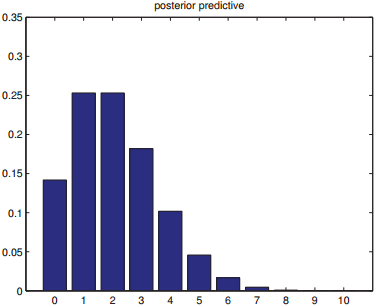
\includegraphics[scale=.60]{beta-binomial-distribution-a.png}} \\
\subfloat[]{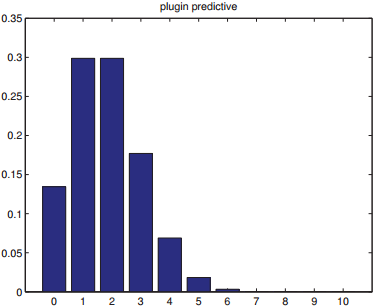
\includegraphics[scale=.60]{beta-binomial-distribution-b.png}}
\caption{(a) Posterior predictive distributions after seeing $N_1=3,N_0=17$. (b) MAP estimation.}
\label{fig:beta-binomial-distribution} 
\end{figure}


\section{The Dirichlet-multinomial model}
In the previous section, we discussed how to infer the probability that a coin comes up heads. In this section, we generalize these results to infer the probability that a dice with $K$ sides comes up as face $k$. 


\subsection{Likelihood}
Suppose we observe $N$ dice rolls, $\mathcal{D}=\{x_1,x_2,\cdots,x_N\}$, where $x_i \in \{1,2,\cdots,K\}$. The likelihood has the form
\begin{equation}
p(\mathcal{D}|\vec{\theta}) = \dbinom{N}{N_1 \cdots N_k} \prod\limits_{k=1}^K\theta_k^{N_k} \quad \text{where } N_k=\sum\limits_{i=1}^N \mathbb{I}(y_i=k)
\end{equation}
almost the same as Equation \ref{eqn:multinomial-pmf}.


\subsection{Prior}
\begin{equation}
\text{Dir}(\vec{\theta}|\vec{\alpha}) = \dfrac{1}{B(\vec{\alpha})}\prod\limits_{k=1}^K \theta_k^{\alpha_k-1}\mathbb{I}(\vec{\theta} \in S_K)
\end{equation}


\subsection{Posterior}
\begin{align}
p(\vec{\theta}|\mathcal{D})& \propto p(\mathcal{D}|\vec{\theta})p(\vec{\theta}) \\
     & \propto \prod\limits_{k=1}^K\theta_k^{N_k}\theta_k^{\alpha_k-1} = \prod\limits_{k=1}^K\theta_k^{N_k+\alpha_k-1}\\
	 & =\text{Dir}(\vec{\theta}|\alpha_1+N_1,\cdots,\alpha_K+N_K)
\end{align}

From Equation \ref{eqn:Dirichlet-properties}, the MAP estimate is given by
\begin{equation}\label{eqn:Dir-MAP}
\hat{\theta}_k=\dfrac{N_k+\alpha_k-1}{N+\alpha_0-K}
\end{equation}

If we use a uniform prior, $\alpha_k=1$, we recover the MLE:
\begin{equation}\label{eqn:Dirichlet-multinomial-posterior-MLE}
\hat{\theta}_k=\dfrac{N_k}{N}
\end{equation}


\subsection{Posterior predictive distribution}
The posterior predictive distribution for a single multinoulli trial is given by the following expression:
\begin{align}
p(X=j|\mathcal{D})& =\int p(X=j|\vec{\theta})p(\vec{\theta}|\mathcal{D})\mathrm{d}\vec{\theta} \\
    & =\int p(X=j|\theta_j)\left[\int p(\vec{\theta}_{-j}, \theta_j|\mathcal{D})\mathrm{d}\vec{\theta}_{-j}\right]\mathrm{d}\theta_j \\
	& =\int \theta_jp(\theta_j|\mathcal{D})\mathrm{d}\theta_j=\mathbb{E}[\theta_j|\mathcal{D}]=\dfrac{\alpha_j+N_j}{\alpha_0+N}
\end{align}
where $\vec{\theta}_{-j}$ are all the components of \vec{\theta} except $\theta_j$.

The above expression avoids the zero-count problem. In fact, this form of Bayesian smoothing is even more important in the multinomial case than the binary case, since the likelihood of data sparsity increases once we start partitioning the data into many categories.


\section{Naive Bayes classifiers}
\label{sec:NBC}
Assume the features are \textbf{conditionally independent} given the class label, then the class conditional density has the following form
\begin{equation}
p(\vec{x}|y=c,\vec{\theta})=\prod\limits_{j=1}^D p(x_j|y=c,\vec{\theta}_{jc})
\end{equation}

The resulting model is called a \textbf{naive Bayes classifier}(NBC).

The form of the class-conditional density depends on the type of each feature. We give some possibilities below:
\begin{itemize}
\item{In the case of real-valued features, we can use the Gaussian distribution: $p(\vec{x}|y,\vec{\theta})=\prod_{j=1}^D \mathcal{N}(x_j|\mu_{jc},\sigma_{jc}^2)$, where $\mu_{jc}$ is the mean of feature $j$ in objects of class $c$, and $\sigma_{jc}^2$ is its variance.}
\item{In the case of binary features, $x_j \in \{0,1\}$, we can use the Bernoulli distribution: $p(\vec{x}|y,\vec{\theta})=\prod_{j=1}^D \text{Ber}(x_j|\mu_{jc})$, where $\mu_{jc}$ is the probability that feature $j$ occurs in class $c$. This is sometimes called the \textbf{multivariate Bernoulli naive Bayes} model. We will see an application of this below.}
\item{In the case of categorical features, $x_j \in \{a_{j1},a_{j2},\cdots, a_{jS_j}\}$, we can use the multinoulli distribution: $p(\vec{x}|y,\vec{\theta})=\prod_{j=1}^D \text{Cat}(x_j|\vec{\mu}_{jc})$, where $\vec{\mu}_{jc}$ is a histogram over the $K$ possible values for $x_j$ in class $c$.}
\end{itemize}

Obviously we can handle other kinds of features, or use different distributional assumptions. Also, it is easy to mix and match features of different types.


\subsection{Optimization}
\label{sec:NBC-Optimization}
We now discuss how to “train” a naive Bayes classifier. This usually means computing the MLE or the MAP estimate for the parameters. However, we will also discuss how to compute the full posterior, $p(\vec{\theta}|\mathcal{D})$.

\subsubsection{MLE for NBC}
The probability for a single data case is given by
\begin{equation}\begin{split}
p(\vec{x}_i,y_i|\vec{\theta}) & =p(y_i|\vec{\pi})\prod\limits_j p(x_{ij}|\vec{\theta}_j) \\
  & =\prod\limits_c \pi_c^{\mathbb{I}(y_i=c)} \prod\limits_j\prod\limits_c p(x_{ij}|\vec{\theta}_{jc})^{\mathbb{I}(y_i=c)}
\end{split}\end{equation}

Hence the log-likelihood is given by
\begin{equation}
p(\mathcal{D}|\vec{\theta})=\sum\limits_{c=1}^C{N_c\log\pi_c}+ \sum\limits_{j=1}^D{\sum\limits_{c=1}^C{\sum\limits_{i:y_i=c}{\log p(x_{ij}|\vec{\theta}_{jc})}}}
\end{equation}
where $N_c \triangleq \sum\limits_i \mathbb{I}(y_i=c)$ is the number of feature vectors in class $c$.

We see that this expression decomposes into a series of terms, one concerning $\vec{\pi}$, and $DC$ terms containing the $\theta_{jc}$’s. Hence we can optimize all these parameters separately.

From Equation \ref{eqn:Dirichlet-multinomial-posterior-MLE}, the MLE for the class prior is given by
\begin{equation}
\hat{\pi}_c=\dfrac{N_c}{N}
\end{equation}

The MLE for $\theta_{jc}$’s depends on the type of distribution we choose to use for each feature. 

In the case of binary features, $x_j \in \{0,1\}$, $x_j|y=c \sim \text{Ber}(\theta_{jc})$, hence
\begin{equation}
\hat{\theta}_{jc}=\dfrac{N_{jc}}{N_c}
\end{equation}
where $N_{jc} \triangleq \sum\limits_{i:y_i=c} \mathbb{I}(y_i=c)$ is the number that feature $j$ occurs in class $c$.

In the case of categorical features, $x_j \in \{a_{j1},a_{j2},\cdots, a_{jS_j}\}$, $x_j|y=c \sim \text{Cat}(\vec{\theta}_{jc})$, hence
\begin{equation}
\hat{\vec{\theta}}_{jc}=(\dfrac{N_{j1c}}{N_c},\dfrac{N_{j2c}}{N_c}, \cdots, \dfrac{N_{jS_j}}{N_c})^T
\end{equation}
where $N_{jkc} \triangleq \sum\limits_{i=1}^N \mathbb{I}(x_{ij}=a_{jk}, y_i=c)$ is the number that feature $x_j=a_{jk}$ occurs in class $c$.


\subsubsection{Bayesian naive Bayes}
\label{sec:Bayesian-naive-Bayes}
Use a Dir$(\vec{\alpha})$ prior for $\vec{\pi}$.

In the case of binary features, use a Beta$(\beta0,\beta1)$ prior for each $\theta_{jc}$; in the case of categorical features, use a Dir$(\vec{\alpha})$ prior for each  $\vec{\theta}_{jc}$. Often we just take $\vec{\alpha}=\vec{1}$ and $\vec{\beta}=\vec{1}$, corresponding to \textbf{add-one} or \textbf{Laplace smoothing}.


\subsection{Using the model for prediction}
The goal is to compute
\begin{equation}\begin{split}
y=f(\vec{x}) & =\arg\max\limits_{c}{P(y=c|\vec{x},\vec{\theta})} \\
   & =P(y=c|\vec{\theta})\prod_{j=1}^D P(x_j|y=c,\vec{\theta})
\end{split}\end{equation}

We can the estimate parameters using MLE or MAP, then the posterior predictive density is obtained by simply plugging in the parameters $\bar{\vec{\theta}}$(MLE) or $\hat{\vec{\theta}}$(MAP). 

Or we can use BMA, just integrate out the unknown parameters.


\subsection{The log-sum-exp trick}
when using generative classifiers of any kind, computing the posterior over class labels using Equation \ref{eqn:Generative-classifier} can fail due to \textbf{numerical underflow}. The problem is that $p(\vec{x}|y=c)$ is often a very small number, especially if \vec{x} is a high-dimensional vector. This is because we require that $\sum_{\vec{x}}p(\vec{x}|y)=1$, so the probability of observing any particular high-dimensional vector is small. The obvious solution is to take logs when applying Bayes rule, as follows:
\begin{equation}
\log p(y=c|\vec{x},\vec{\theta})=b_c-\log\left(\sum\limits_{c'}e^{b_{c'}}\right)
\end{equation}
where $b_c \triangleq \log p(\vec{x}|y=c,\vec{\theta})+\log p(y=c|\vec{\theta})$.

We can factor out the largest term, and just represent the remaining numbers relative to that. For example,
\begin{equation}\begin{split}
\log(e^{-120}+e^{-121}) & =\log(e^{-120}(1+e^{-1})) \\
   & =\log(1+e^{-1})-120
\end{split}\end{equation}

In general, we have
\begin{equation}
\sum\limits_{c}e^{b_{c}}=\log\left[(\sum e^{b_c-B})e^B\right]=\log\left(\sum e^{b_c-B}\right)+B
\end{equation}
where $B \triangleq \max\{b_c\}$.

This is called the \textbf{log-sum-exp} trick, and is widely used. 


\subsection{Feature selection using mutual information}
Since an NBC is fitting a joint distribution over potentially many features, it can suffer from overfitting. In addition, the run-time cost is $O(D)$, which may be too high for some applications. 

One common approach to tackling both of these problems is to perform \textbf{feature selection}, to remove “irrelevant” features that do not help much with the classification problem. The simplest approach to feature selection is to evaluate the relevance of each feature separately, and then take the top K,whereKis chosen based on some tradeoff between accuracy and complexity. This approach is known as \textbf{variable ranking}, \textbf{filtering}, or \textbf{screening}.

One way to measure relevance is to use mutual information (Section \ref{sec:Mutual-information}) between feature $X_j$ and the class label $Y$
\begin{equation}
\mathbb{I}(X_j,Y)=\sum\limits_{x_j}{\sum\limits_{y}{p(x_j,y)\log \dfrac{p(x_j,y)}{p(x_j)p(y)}}}
\end{equation}

If the features are binary, it is easy to show that the MI can be computed as follows
\begin{equation}
\mathbb{I}_j = \sum\limits_c \left[\theta_{jc}\pi_c\log{\dfrac{\theta_{jc}}{\theta_j}}+(1-\theta_{jc})\pi_c\log{\dfrac{1-\theta_{jc}}{1-\theta_j}}\right]
\end{equation}
where $\pi_c=p(y=c)$, $\theta_{jc}=p(x_j=1|y=c)$, and $\theta_j=p(x_j=1)=\sum_{c} \pi_c\theta_{jc}$.


\subsection{Classifying documents using bag of words}
\textbf{Document classification} is the problem of classifying text documents into different categories.


\subsubsection{Bernoulli product model}
One simple approach is to represent each document as a binary vector, which records whether each word is present or not, so $x_{ij} =1$ iff word $j$ occurs in document $i$, otherwise $x_{ij}=0$. We can then use the following class conditional density:
\begin{equation}\begin{split}
p(\vec{x}_i|y_i=c,\vec{\theta}) & =\prod\limits_{j=1}^D \mathrm{Ber}(x_{ij}|\theta_{jc}) \\
  & =\prod\limits_{j=1}^D \theta_{jc}^{x_{ij}}(1-\theta_{jc})^{1-x_{ij}}
\end{split}\end{equation}

This is called the \textbf{Bernoulli product model}, or the \textbf{binary independence model}.

\subsubsection{Multinomial document classifier}
However, ignoring the number of times each word occurs in a document loses some information (McCallum and Nigam 1998). A more accurate representation counts the number of occurrences of each word. Specifically, let $\vec{x}_i$ be a vector of counts for document $i$, so $x_{ij} \in \{0,1,\cdots,N_i\}$, where $N_i$ is the number of terms in document $i$(so $\sum\limits_{j=1}^D x_{ij}=N_i$). For the class conditional densities, we can use a multinomial distribution:
\begin{equation}\label{eqn:Multinomial-document-classifier}
p(\vec{x}_i|y_i=c,\vec{\theta})=\text{Mu}(\vec{x}_i|N_i,\vec{\theta}_c)=\dfrac{N_i!}{\prod_{j=1}^D x_{ij}!}\prod\limits_{j=1}^D \theta_{jc}^{x_{ij}}
\end{equation}
where we have implicitly assumed that the document length $N_i$ is independent of the class. Here $θ_{jc}$ is the probability of generating word $j$ in documents of class $c$; these parameters satisfy the constraint that $\sum_{j=1}^D \theta_{jc}=1$ for each class c.

Although the multinomial classifier is easy to train and easy to use at test time, it does not work particularly well for document classification. One reason for this is that it does not take into account the \textbf{burstiness} of word usage. This refers to the phenomenon that most words never appear in any given document, but if they do appear once, they are likely to appear more than once, i.e., words occur in bursts.

The multinomial model cannot capture the burstiness phenomenon. To see why, note that Equation \ref{eqn:Multinomial-document-classifier} has the form $\theta_{jc}^{x_{ij}}$, and since $\theta_{jc} \ll 1$ for rare words, it becomes increasingly unlikely to generate many of them. For more frequent words, the decay rate is not as fast. To see why intuitively, note that the most frequent words are function words which are not specific to the class, such as “and”, “the”, and “but”; the chance of the word “and” occuring is pretty much the same no matter how many time it has previously occurred (modulo document length), so the independence assumption is more reasonable for common words. However, since rare words are the ones that matter most for classification purposes, these are the ones we want to model the most carefully.

\subsubsection{DCM model}
Various ad hoc heuristics have been proposed to improve the performance of the multinomial document classifier (Rennie et al. 2003). We now present an alternative class conditional density that performs as well as these ad hoc methods, yet is probabilistically sound (Madsen et al. 2005).

Suppose we simply replace the multinomial class conditional density with the \textbf{Dirichlet Compound Multinomial} or \textbf{DCM} density, defined as follows:
\begin{equation}\begin{split}
p(\vec{x}_i|y_i=c,\vec{\alpha}) & =\int \text{Mu}(\vec{x}_i|N_i,\vec{\theta}_c)\text{Dir}(\vec{\theta}_c|\vec{\alpha}_c) \\
   & =\dfrac{N_i!}{\prod_{j=1}^D x_{ij}!}\prod\limits_{j=1}^D\dfrac{B(\vec{x}_i+\vec{\alpha}_c)}{B(\vec{\alpha}_c)}
\end{split}\end{equation}

(This equation is derived in Equation TODO.) Surprisingly this simple change is all that is needed to capture the burstiness phenomenon. The intuitive reason for this is as follows: After seeing one occurence of a word, say wordj, the posterior counts on θj gets updated, making another occurence of wordjmore likely. By contrast, ifθj is fixed, then the occurences of each word are independent. The multinomial model corresponds to drawing a ball from an urn with Kcolors of ball, recording its color, and then replacing it. By contrast, the DCM model corresponds to drawing a ball, recording its color, and then replacing it with one additional copy; this is called the \textbf{Polya urn}.

Using the DCM as the class conditional density gives much better results than using the multinomial, and has performance comparable to state of the art methods, as described in (Madsen et al. 2005). The only disadvantage is that fitting the DCM model is more complex; see (Minka 2000e; Elkan 2006) for the details.

\chapter{Gaussian Models}
\label{chap:Gaussian Models}
The Gaussian,also known as the \textbf{normal distribution},is a widely used model for the \textbf{distribution of continuous variables}.In the case of a single variable $x$,the Gaussian distribution can be written in the form
\begin{equation}
	\mathcal{N}(x|\mu,\sigma^2) = \dfrac{1}{(2\pi\sigma^2)^{\frac{1}{2}}}\exp\{\dfrac{1}{2\sigma^2 (x-\mu)^2} \}
\end{equation}
where the $\mu$ is the mean and $\sigma^2$ is the variance.
Now we will discuss the \textbf{multivariate Gaussian} or \textbf{multivariate normal(MVN)}, which is the most widely used joint probability density function for continuous variables. It will form the basis for many of the models.


\section{Gaussian discriminant analysis}
One important application of MVNs is to define the the class conditional densities in a generative classifier, i.e.,
\begin{equation}
p(\vec{x}|y=c,\vec{\theta})=\mathcal{N}(\vec{x}|\vec{\mu}_c,\vec{\Sigma}_c)
\end{equation}

The resulting technique is called (Gaussian) \textbf{discriminant analysis} or \textbf{GDA} (even though it is a generative, not discriminative, classifier — see Section TODO for more on this distinction). If $\vec{\Sigma}_c$ is diagonal, this is equivalent to naive Bayes.

We can classify a feature vector using the following decision rule, derived from Equation \ref{eqn:Generative-classifier}:
\begin{equation}
y=\arg\max_{c} \left[\log p(y=c|\vec{\pi})+\log p(\vec{x}|\vec{\theta})\right]
\end{equation}

When we compute the probability of $\vec{x}$ under each class conditional density, we are measuring the distance from $\vec{x}$ to the center of each class, $\vec{\mu}_c$, using Mahalanobis distance. This can be thought of as a \textbf{nearest centroids classifier}.

\begin{figure}[hbtp]
\centering
\subfloat[]{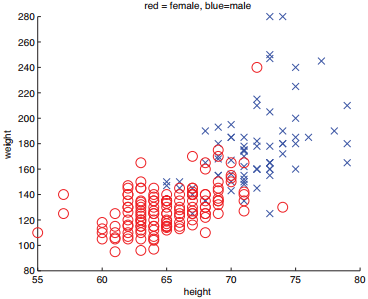
\includegraphics[scale=.70]{2d-Gaussians-Visualization-a.png}} \\
\subfloat[]{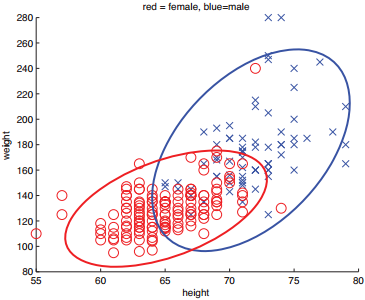
\includegraphics[scale=.70]{2d-Gaussians-Visualization-b.png}}
\caption{(a) Height/weight data. (b) Visualization of 2d Gaussians fit to each class. 95\% of the probability mass is inside the ellipse.}
\label{fig:2d-Gaussians-Visualization} 
\end{figure}

As an example, Figure \ref{fig:2d-Gaussians-Visualization} shows two Gaussian class-conditional densities in 2d, representing the height and weight of men and women. We can see that the features are correlated, as is to be expected (tall people tend to weigh more). The ellipses for each class contain 95\% of the probability mass. If we have a uniform prior over classes, we can classify a new test vector as follows:
\begin{equation}
y=\arg\max_{c} (\vec{x}-\vec{\mu}_c)^T\vec{\Sigma}_c^{-1}(\vec{x}-\vec{\mu}_c)
\end{equation}


\subsection{Quadratic discriminant analysis (QDA)}
By plugging in the definition of the Gaussian density to Equation \ref{eqn:Generative-classifier}, we can get
\begin{equation}\label{eqn:QDA}
p(y|\vec{x},\vec{\theta})=\dfrac{\pi_c|2\pi\vec{\Sigma}_c|^{-\frac{1}{2}}\exp\left[-\frac{1}{2}(\vec{x}-\vec{\mu})^T\vec{\Sigma}^{-1}(\vec{x}-\vec{\mu})\right]}{\sum_{c'}\pi_{c'}|2\pi\vec{\Sigma}_{c'}|^{-\frac{1}{2}}\exp\left[-\frac{1}{2}(\vec{x}-\vec{\mu})^T\vec{\Sigma}^{-1}(\vec{x}-\vec{\mu})\right]}
\end{equation}

Thresholding this results in a quadratic function of $\vec{x}$. The result is known as quadratic discriminant analysis(QDA). Figure \ref{fig:QDA} gives some examples of what the decision boundaries look like in 2D.

\begin{figure}[hbtp]
\centering
\subfloat[]{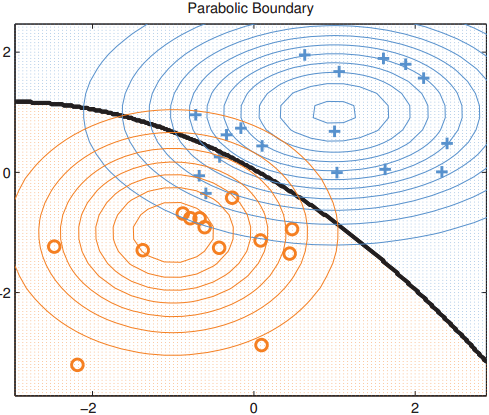
\includegraphics[scale=.50]{QDA-a.png}} \\
\subfloat[]{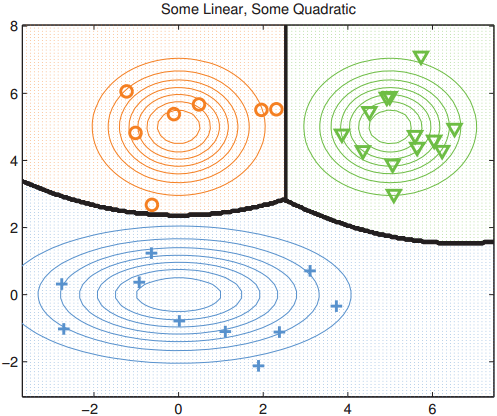
\includegraphics[scale=.50]{QDA-b.png}}
\caption{Quadratic decision boundaries in 2D for the 2 and 3 class case.}
\label{fig:QDA} 
\end{figure}


\subsection{Linear discriminant analysis (LDA)}
\label{sec:Linear-discriminant-analysis}
We now consider a special case in which the covariance matrices are \textbf{tied} or \textbf{shared} across classes,$\vec{\Sigma}_c=\vec{\Sigma}$. In this case, we can simplify Equation \ref{eqn:QDA} as follows:
\begin{align}
p(y|\vec{x},\vec{\theta})& \propto \pi_c\exp\left(\vec{\mu}_c\vec{\Sigma}^{-1}\vec{x}-\dfrac{1}{2}\vec{x}^T\vec{\Sigma}^{-1}\vec{x}-\dfrac{1}{2}\vec{\mu}_c^T\vec{\Sigma}^{-1}\vec{\mu}_c\right) \nonumber \\
 & =\exp\left(\vec{\mu}_c\vec{\Sigma}^{-1}\vec{x}-\dfrac{1}{2}\vec{\mu}_c^T\vec{\Sigma}^{-1}\vec{\mu}_c+\log \pi_c\right) \nonumber \\
 & \quad \exp\left(-\dfrac{1}{2}\vec{x}^T\vec{\Sigma}^{-1}\vec{x}\right) \nonumber \\
 & \propto \exp\left(\vec{\mu}_c\vec{\Sigma}^{-1}\vec{x}-\dfrac{1}{2}\vec{\mu}_c^T\vec{\Sigma}^{-1}\vec{\mu}_c+\log \pi_c\right)
\end{align}

Since the quadratic term $\vec{x}^T\vec{\Sigma}^{-1}\vec{x}$ is independent of $c$, it will cancel out in the numerator and denominator. If we define
\begin{align}
\gamma_c& \triangleq -\dfrac{1}{2}\vec{\mu}_c^T\vec{\Sigma}^{-1}\vec{\mu}_c+\log \pi_c \\
\vec{\beta}_c& \triangleq \vec{\Sigma}^{-1}\vec{\mu}_c
\end{align}
then we can write
\begin{equation}\label{eqn:LDA}
p(y|\vec{x},\vec{\theta})=\dfrac{e^{\vec{\beta}_c^T\vec{x}+\gamma_c}}{\sum_{c'}e^{\vec{\beta}_{c'}^T\vec{x}+\gamma_{c'}}} \triangleq \sigma(\vec{\eta}, c)
\end{equation}
where $\vec{\eta} \triangleq (e^{\vec{\beta}_1^T\vec{x}}+\gamma_1,\cdots, e^{\vec{\beta}_C^T\vec{x}}+\gamma_C)$, $\sigma()$ is the \textbf{softmax activation function}\footnote{\url{http://en.wikipedia.org/wiki/Softmax_activation_function}}, defined as follows:
\begin{equation}
\sigma(\vec{q},i) \triangleq \dfrac{\exp(q_i)}{\sum_{j=1}^n \exp(q_j)}
\end{equation}

When parameterized by some constant, $\alpha > 0$, the following formulation becomes a smooth, differentiable approximation of the maximum function:
\begin{equation}
\mathcal{S}_{\alpha}(\vec{x}) = \dfrac{\sum_{j=1}^D x_je^{\alpha x_j}}{\sum_{j=1}^D e^{\alpha x_j}}
\end{equation}

$\mathcal{S}_{\alpha}$ has the following properties:
\begin{enumerate}
\item $\mathcal{S}_{\alpha} \rightarrow \max$ as $\alpha \rightarrow \infty$
\item $\mathcal{S}_0$ is the average of its inputs
\item $\mathcal{S}_{\alpha} \rightarrow \min$ as $\alpha \rightarrow -\infty$
\end{enumerate}

Note that the softmax activation function comes from the area of statistical physics, where it is common to use the \textbf{Boltzmann distribution}, which has the same form as the softmax activation function.

An interesting property of Equation \ref{eqn:LDA} is that, if we take logs, we end up with a linear function of $\vec{x}$. (The reason it is linear is because the $\vec{x}^T\vec{\Sigma}^{-1}\vec{x}$ cancels from the numerator and denominator.) Thus the decision boundary between any two classes, says $c$ and $c'$, will be a straight line. Hence this technique is called \textbf{linear discriminant analysis} or \textbf{LDA}.

An alternative to fitting an LDA model and then deriving the class posterior is to directly fit $p(y|\vec{x},\vec{W})=\text{Cat}(y|\vec{W}\vec{x})$ for some $C \times D$ weight matrix $\vec{W}$. This is called \textbf{multi-class logistic regression}, or \textbf{multinomial logistic regression}. We will discuss this model in detail in Section TODO. The difference between the two approaches is explained in Section TODO.


\subsection{Two-class LDA}
To gain further insight into the meaning of these equations, let us consider the binary case. In this case, the posterior is given by
\begin{align}
p(y=1|\vec{x},\vec{\theta})& =\dfrac{e^{\vec{\beta}_1^T\vec{x}+\gamma_1}}{e^{\vec{\beta}_0^T\vec{x}+\gamma_0}+e^{\vec{\beta}_1^T\vec{x}+\gamma_1}}) \\
  & =\dfrac{1}{1+e^(\vec{\beta}_0-\vec{\beta}_1)^T\vec{x}+(\gamma_0-\gamma_1)} \\
  & =\text{sigm}((\vec{\beta}_1-\vec{\beta}_0)^T\vec{x}+(\gamma_0-\gamma_1))
\end{align}
where sigm$(x)$ refers to the sigmoid function\footnote{\url{http://en.wikipedia.org/wiki/Sigmoid_function}}.

Now
\begin{align}
\gamma_1-\gamma_0& = -\dfrac{1}{2}\vec{\mu}_1^T\vec{\Sigma}^{-1}\vec{\mu}_1+\dfrac{1}{2}\vec{\mu}_0^T\vec{\Sigma}^{-1}\vec{\mu}_0 + \log(\pi_1/\pi_0) \\
 & =-\dfrac{1}{2}(\vec{\mu}_1-\vec{\mu}_0)^T\vec{\Sigma}^{-1}(\vec{\mu}_1+\vec{\mu}_0)+ \log(\pi_1/\pi_0)
\end{align}

So if we define
\begin{align}
\vec{w}& =\vec{\beta}_1-\vec{\beta}_0=\vec{\Sigma}^{-1}(\vec{\mu}_1-\vec{\mu}_0) \\
\vec{x}_0& =\dfrac{1}{2}(\vec{\mu}_1+\vec{\mu}_0)-(\vec{\mu}_1-\vec{\mu}_0)\dfrac{\log(\pi_1/\pi_0)}{(\vec{\mu}_1-\vec{\mu}_0)^T\vec{\Sigma}^{-1}(\vec{\mu}_1-\vec{\mu}_0)}
\end{align}
then we have $\vec{w}^T\vec{x}_0=-(\gamma_1-\gamma_0)$, and hence
\begin{equation}
p(y=1|\vec{x},\vec{\theta})=\text{sigm}(\vec{w}^T(\vec{x}-\vec{x}_0))
\end{equation}

(This is closely related to logistic regression, which we will discuss in Section TODO.) So the final decision rule is as follows: shift $\vec{x}$ by $\vec{x}_0$, project onto the line \vec{w}, and see if the result is positive or negative.

\begin{figure}[hbtp]
\centering
    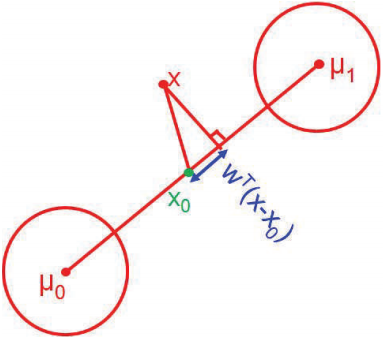
\includegraphics[scale=.50]{2d-LDA.png}
\caption{Geometry of LDA in the 2 class case where $\vec{\Sigma}_1=\vec{\Sigma}_2=\vec{I}$.}
\label{fig:2d-LDA} 
\end{figure}

If $\vec{\Sigma}=\sigma^2\vec{I}$, then $\vec{w}$ is in the direction of $\vec{\mu}_1-\vec{\mu}_0$. So we classify the point based on whether its projection is closer to $\vec{\mu}_0$ or $\vec{\mu}_1$ . This is illustrated in Figure \ref{fig:2d-LDA}. Furthemore, if $\vec{\pi}_1=\vec{\pi}_0$, then $\vec{x}_0=\frac{1}{2}(\vec{\mu}_1+\vec{\mu}_0)$, which is half way between the means. If we make $\vec{\pi}_1>\vec{\pi}_0$, then $\vec{x}_0$ gets closer to $\vec{\mu}_0$, so more of the line belongs to class 1 a \emph{priori}. Conversely if $\vec{\pi}_1<\vec{\pi}_0$, the boundary shifts right. Thus we see that the class prior, πc, just changes the decision threshold, and not the overall geometry, as we claimed above. (A similar argument applies in the multi-class case.)

The magnitude of $\vec{w}$ determines the steepness of the logistic function, and depends on how well-separated the means are, relative to the variance. In psychology and signal detection theory, it is common to define the \textbf{discriminability} of a signal from the background noise using a quantity called \textbf{d-prime}:
\begin{equation}
d' \triangleq \dfrac{\mu_1-\mu_0}{\sigma}
\end{equation}
where $\mu_1$ is the mean of the signal and $\mu_0$ is the mean of the noise, and $\sigma$ is the standard deviation of the noise. If $d'$ is large, the signal will be easier to discriminate from the noise.


\subsection{MLE for discriminant analysis}
\label{sec:MLE-for-discriminant-analysis}
The log-likelihood function is as follows:
\begin{equation}
p(\mathcal{D}|\vec{\theta})=\sum\limits_{c=1}^C{\sum\limits_{i:y_i=c}{\log\pi_c}}+\sum\limits_{c=1}^C{\sum\limits_{i:y_i=c}{\log\mathcal{N}(\vec{x}_i|\vec{\mu}_c,\vec{\Sigma}_c)}}
\end{equation}

The MLE for each parameter is as follows:
\begin{align}
\bar{\vec{\mu}}_c& = \dfrac{N_c}{N} \\
\bar{\vec{\mu}}_c& = \dfrac{1}{N_c}\sum\limits_{i:y_i=c}\vec{x}_i \\
\bar{\vec{\Sigma}}_c& = \dfrac{1}{N_c}\sum\limits_{i:y_i=c}(\vec{x}_i-\bar{\vec{\mu}}_c)(\vec{x}_i-\bar{\vec{\mu}}_c)^T
\end{align}


\subsection{Strategies for preventing overfitting}
The speed and simplicity of the MLE method is one of its greatest appeals. However, the MLE can badly overfit in high dimensions. In particular, the MLE for a full covariance matrix is singular if $N_c <D$. And even when $N_c >D$, the MLE can be ill-conditioned, meaning it is close to singular. There are several possible solutions to this problem:
\begin{itemize}
\item{Use a diagonal covariance matrix for each class, which assumes the features are conditionally independent; this is equivalent to using a naive Bayes classifier (Section \ref{sec:NBC})}.
\item{Use a full covariance matrix, but force it to be the same for all classes,$\vec{\Sigma}_c=\vec{\Sigma}$. This is an example of \textbf{parameter tying} or \textbf{parameter sharing}, and is equivalent to LDA (Section \ref{sec:Linear-discriminant-analysis}).}
\item{Use a diagonal covariance matrix and forced it to be shared. This is called diagonal covariance LDA, and is discussed in Section TODO.}
\item{Use a full covariance matrix, but impose a prior and then integrate it out. If we use a conjugate prior, this can be done in closed form, using the results from Section TODO; this is analogous to the “Bayesian naive Bayes” method in Section \ref{sec:Bayesian-naive-Bayes}. See (Minka 2000f) for details.}
\item{Fit a full or diagonal covariance matrix by MAP estimation. We discuss two different kindsof prior below.}
\item{Project the data into a low dimensional subspace and fit the Gaussians there. See Section TODO for a way to find the best (most discriminative) linear projection.}
\end{itemize}

We discuss some of these options below.


\subsection{Regularized LDA *}


\subsection{Diagonal LDA}


\subsection{Nearest shrunken centroids classifier *}
One drawback of diagonal LDA is that it depends on all of the features. In high dimensional problems, we might prefer a method that only depends on a subset of the features, for reasons of accuracy and interpretability. One approach is to use a screening method, perhaps based on mutual information, as in Section 3.5.4. We now discuss another approach to this problem known as the \textbf{nearest shrunken centroids} classifier (Hastie et al. 2009, p652).


\section{Inference in jointly Gaussian distributions}
\label{sec:Inference-in-jointly-Gaussian-distributions}
Given a joint distribution, $p(\vec{x}_1,\vec{x}_2)$, it is useful to be able to compute marginals $p(\vec{x}_1)$ and conditionals $p(\vec{x}_1|\vec{x}_2)$. We discuss how to do this below, and then give some applications. These operations take $O(D^3)$ time in the worst case. See Section TODO for faster methods.


\subsection{Statement of the result}

\begin{theorem}(\textbf{Marginals and conditionals of an MVN}). Suppose $X=(\vec{x}_1,\vec{x}_2)$is jointly Gaussian with parameters
\begin{equation}
\vec{\mu}=\left(\begin{array}{c}\vec{\mu}_1 \\
                                \vec{\mu}_2\end{array}\right),
\vec{\Sigma}=\left(\begin{array}{cc}
                   \vec{\Sigma}_{11} & \vec{\Sigma}_{12} \\
 				   \vec{\Sigma}_{21} & \vec{\Sigma}_{22} \end{array}\right),
\vec{\Lambda}=\vec{\Sigma}^{-1}=\left(\begin{array}{cc}
                   \vec{\Lambda}_{11} & \vec{\Lambda}_{12} \\
 				   \vec{\Lambda}_{21} & \vec{\Lambda}_{22} \end{array}\right),
\end{equation}

Then the marginals are given by
\begin{equation}
\begin{split}
p(\vec{x}_1)= \mathcal{N}(\vec{x}_1|\vec{\mu}_1,\vec{\Sigma}_{11})\\
p(\vec{x}_2)= \mathcal{N}(\vec{x}_2|\vec{\mu}_2,\vec{\Sigma}_{22})
\end{split}
\end{equation}
and the posterior conditional is given by
\begin{equation}\label{eqn:Marginals-and-conditionals-of-an-MVN}
  \boxed{\begin{split}
    p(\vec{x}_1|\vec{x}_2)& =\mathcal{N}(\vec{x}_1|\vec{\mu}_{1|2},\vec{\Sigma}_{1|2}) \\
    \vec{\mu}_{1|2}& = \vec{\mu}_1+\vec{\Sigma}_{12}\vec{\Sigma}_{22}^{-1}(\vec{x}_2-\vec{\mu}_2) \\
	               & = \vec{\mu}_1-\vec{\Lambda}_{11}^{-1}\vec{\Lambda}_{12}(\vec{x}_2-\vec{\mu}_2) \\
				   & = \vec{\Sigma}_{1|2}(\vec{\Lambda}_{11}\vec{\mu}_1-\vec{\Lambda}_{12}(\vec{x}_2-\vec{\mu}_2)) \\
	\vec{\Sigma}_{1|2}& = \vec{\Sigma}_{11}-\vec{\Sigma}_{12}\vec{\Sigma}_{22}^{-1}\vec{\Sigma}_{21}=\vec{\Lambda}_{11}^{-1}
  \end{split}}
\end{equation}
\end{theorem}

Equation \ref{eqn:Marginals-and-conditionals-of-an-MVN} is of such crucial importance in this book that we have put a box around it, so you can easily find it. For the proof, see Section TODO.

We see that both the marginal and conditional distributions are themselves Gaussian. For the marginals, we just extract the rows and columns corresponding to $\vec{x}_1$ or $\vec{x}_2$. For the conditional, we have to do a bit more work. However, it is not that complicated: the conditional mean is just a linear function of $\vec{x}_2$, and the conditional covariance is just a constant matrix that is independent of $\vec{x}_2$. We give three different (but equivalent) expressions for the posterior mean, and two different (but equivalent) expressions for the posterior covariance; each one is useful in different circumstances.


\subsection{Examples}
Below we give some examples of these equations in action, which will make them seem more intuitive.


\subsubsection{Marginals and conditionals of a 2d Gaussian}

\subsection{information form}

\subsection{Proof}

\section{Linear Gaussian systems}
Suppose we have two variables, $\vec{x}$ and $\vec{y}$.Let $\vec{x} \in \mathbb{R}^{D_x}$ be a hidden variable, and $\vec{y} \in \mathbb{R}^{D_y}$ be a noisy observation of $\vec{x}$. Let us assume we have the following prior and likelihood:
\begin{equation}\label{eqn:Linear-Gaussian-system}
  \boxed{\begin{split}
    p(\vec{x})&=\mathcal{N}(\vec{x}|\vec{\mu}_x,\vec{\Sigma}_x) \\
	p(\vec{y}|\vec{x})&=\mathcal{N}(\vec{y}|\vec{W}\vec{x}+\vec{\mu}_y,\vec{\Sigma}_y)
  \end{split}}
\end{equation}
where $\vec{W}$ is a matrix of size $D_y \times D_x$. This is an example of a \textbf{linear Gaussian system}. We can represent this schematically as $\vec{x} \rightarrow \vec{y}$, meaning $\vec{x}$ generates $\vec{y}$. In this section, we show how to “invert the arrow”, that is, how to infer $\vec{x}$ from $\vec{y}$. We state the result below, then give several examples, and finally we derive the result. We will see many more applications of these results in later chapters.


\subsection{Statement of the result}
\begin{theorem}(\textbf{Bayes rule for linear Gaussian systems}). 
Given a linear Gaussian system, as in Equation \ref{eqn:Linear-Gaussian-system}, the posterior $p(\vec{x}|\vec{y})$ is given by the following:
\begin{equation}\label{eqn:Linear-Gaussian-system-posterior}
  \boxed{\begin{split}
    p(\vec{x}|\vec{y})&=\mathcal{N}(\vec{x}|\vec{\mu}_{x|y},\vec{\Sigma}_{x|y}) \\
	\vec{\Sigma}_{x|y}&=\vec{\Sigma}_x^{-1}+\vec{W}^T\vec{\Sigma}_y^{-1}\vec{W} \\
	\vec{\mu}_{x|y}&=\vec{\Sigma}_{x|y}\left[\vec{W}^T\vec{\Sigma}_y^{-1}(\vec{y}-\vec{\mu}_y)+\vec{\Sigma}_x^{-1}\vec{\mu}_x\right]
  \end{split}}
\end{equation}
In addition, the normalization constant $p(\vec{y})$ is given by
\begin{equation}\label{eqn:Linear-Gaussian-system-normalizer}
  \boxed{
    p(\vec{y})=\mathcal{N}(\vec{y}|\vec{W}\vec{\mu}_x+\vec{\mu}_y,\vec{\Sigma}_y+\vec{W}\vec{\Sigma}_x\vec{W}^T)
  }
\end{equation}
\end{theorem}

For the proof, see Section 4.4.3 TODO.

\subsection{Examples}

\subsection{Proof}

\section{Digression: The Wishart distribution *}


\section{Inferring the parameters of an MVN}


\subsection{Posterior distribution of $\mu$}



\subsection{Posterior distribution of $\Sigma$ *}



\subsection{Posterior distribution of $\mu$ and $\Sigma$ *}
\label{sec:Posterior-distribution-of-mu-and-Sigma}


\subsection{Sensor fusion with unknown precisions *}


\chapter{Bayesian statistics}
\label{chap:Bayesian statistics}

\section{Introduction}
Using the posterior distribution to summarize everything we know about a set of unknown variables is at the core of Bayesian statistics. In this chapter, we discuss this approach to statistics in more detail.


\section{Summarizing posterior distributions}
The posterior $p(\vec{\theta}|\mathcal{D})$ summarizes everything we know about the unknown quantities $\vec{\theta}$. In this section, we discuss some simple quantities that can be derived from a probability distribution, such as a posterior. These summary statistics are often easier to understand and visualize than the full joint.


\subsection{MAP estimation}
We can easily compute a \textbf{point estimate} of an unknown quantity by computing the posterior mean, median or mode. In Section \ref{sec:Bayesian-decision-theory}, we discuss how to use decision theory to choose between these methods. Typically the posterior mean or median is the most appropriate choice for a realvalued quantity, and the vector of posterior marginals is the best choice for a discrete quantity. However, the posterior mode, aka the MAP estimate, is the most popular choice because it reduces to an optimization problem, for which efficient algorithms often exist. Futhermore, MAP estimation can be interpreted in non-Bayesian terms, by thinking of the log prior as a regularizer (see Section TODO for more details).

Although this approach is computationally appealing, it is important to point out that there are various drawbacks to MAP estimation, which we briefly discuss below. This will provide motivation for the more thoroughly Bayesian approach which we will study later in this chapter(and elsewhere in this book).


\subsubsection{No measure of uncertainty}
The most obvious drawback of MAP estimation, and indeed of any other \emph{point estimate} such as the posterior mean or median, is that it does not provide any measure of uncertainty. In many applications, it is important to know how much one can trust a given estimate. We can derive such confidence measures from the posterior, as we discuss in Section \ref{sec:Credible-intervals}.

\subsubsection{Plugging in the MAP estimate can result in overfitting}
If we don’t model the uncertainty in our parameters, then our predictive distribution will be overconfident. Overconfidence in predictions is particularly problematic in situations where we may be risk averse; see Section \ref{sec:Bayesian-decision-theory} for details.

\subsubsection{The mode is an untypical point}
Choosing the mode as a summary of a posterior distribution is often a very poor choice, since the mode is usually quite untypical of the distribution, unlike the mean or median. The basic problem is that the mode is a point of measure zero, whereas the mean and median take the volume of the space into account. See Figure \ref{fig:untypical-point}.

\begin{figure}[hbtp]
\centering
\subfloat[]{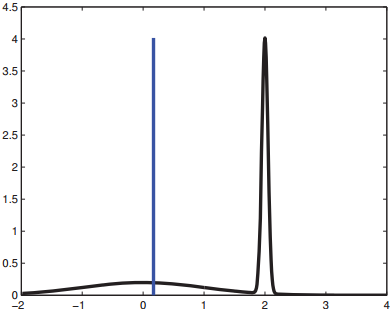
\includegraphics[scale=.50]{untypical-point-a.png}} \\
\subfloat[]{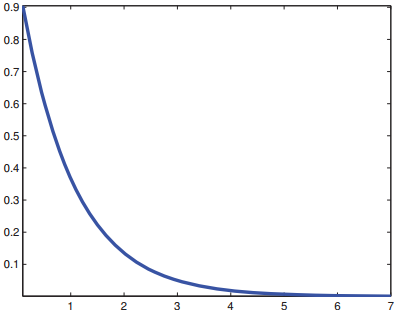
\includegraphics[scale=.50]{untypical-point-b.png}}
\caption{(a) A bimodal distribution in which the mode is very untypical of the distribution. The thin blue vertical line is the mean, which is arguably a better summary of the distribution, since it is near the majority of the probability mass. (b) A skewed distribution in which the mode is quite different from the mean.}
\label{fig:untypical-point} 
\end{figure}

How should we summarize a posterior if the mode is not a good choice? The answer is to use decision theory, which we discuss in Section \ref{sec:Bayesian-decision-theory}. The basic idea is to specify a loss function, where $L(\theta,\hat{\theta})$ is the loss you incur if the truth is $\theta$ and your estimate is $\hat{\theta}$. If we use 0-1 loss $L(\theta,\hat{\theta})=\mathbb{I}(\theta \neq \hat{\theta})$(see section \ref{sec:Loss-function-and-risk-function}), then the optimal estimate is the posterior mode. 0-1 loss means you only get “points” if you make no errors, otherwise you get nothing: there is no “partial credit” under this loss function! For continuous-valued quantities, we often prefer to use squared error loss, $L(\theta,\hat{\theta})=(\theta-\hat{\theta})^2$ ; the corresponding optimal estimator is then the posterior mean, as we show in Section \ref{sec:Bayesian-decision-theory}. Or we can use a more robust loss function, $L(\theta,\hat{\theta})=|\theta-\hat{\theta}|$, which gives rise to the posterior median.

\subsubsection{MAP estimation is not invariant to reparameterization *}
A more subtle problem with MAP estimation is that the result we get depends on how we parameterize the probability distribution. Changing from one representation to another equivalent representation changes the result, which is not very desirable, since the units of measurement are arbitrary (e.g., when measuring distance, we can use centimetres or inches).

To understand the problem, suppose we compute the posterior forx. If we define y=f(x), the distribution for yis given by Equation \ref{eqn:General-transformations}. The $\frac{\mathrm{d}x}{\mathrm{d}y}$ term is called the Jacobian, and it measures the change in size of a unit volume passed
through $f$. Let $\hat{x}=\arg\max_x p_x(x)$ be the MAP estimate for $x$. In general it is not the case that $\hat{x}=\arg\max_x p_x(x)$ is given by $f(\hat{x})$. For example, let $X \sim \mathcal{N}(6,1)$ and $y=f(x)$, where $f(x)=1/(1+\exp(-x+5))$. 

\begin{figure}[hbtp]
\centering
    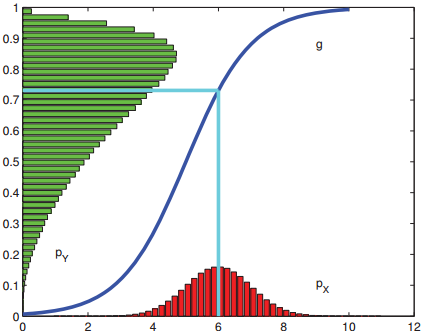
\includegraphics[scale=.70]{mode-reparameterization.png}
\caption{Example of the transformation of a density under a nonlinear transform. Note how the mode of the transformed distribution is not the transform of the original mode. Based on Exercise 1.4 of (Bishop 2006b).}
\label{fig:mode-reparameterization} 
\end{figure}

We can derive the distribution of $y$ using Monte Carlo simulation (see Section \ref{sec:Monte-Carlo-approximation}). The result is shown in Figure \ref{sec:mode-reparameterization}. We see that the original Gaussian has become “squashed” by the sigmoid nonlinearity. In particular, we see that the mode of the transformed distribution is not equal to the transform of the original mode.

The MLE does not suffer from this since the likelihood is a function, not a probability density. Bayesian inference does not suffer from this problem either, since the change of measure is taken into account when integrating over the parameter space.


\subsection{Credible intervals}
\label{sec:Credible-intervals}
In addition to point estimates, we often want a measure of confidence. A standard measure of confidence in some (scalar) quantity $\theta$ is the “width” of its posterior distribution. This can be measured using a $100(1−\alpha)\%$ credible interval, which is a (contiguous) region $C=(\ell,u)$(standing for lower and upper) which contains $1−\alpha$ of the posterior probability mass, i.e.,
\begin{equation}
C_{\alpha}(\mathcal{D}) \quad \text{where } P(\ell \leq \theta \leq u)=1-\alpha
\end{equation}

There may be many such intervals, so we choose one such that there is $(1−\alpha)/2$ mass in each tail; this is called a \textbf{central interval}.

If the posterior has a known functional form, we can compute the posterior central interval using $\ell=F^{-1}(\alpha/2)$ and $u=F^{-1}(1-\alpha/2)$, where $F$ is the cdf of the posterior. 

If we don’t know the functional form, but we can draw samples from the posterior, then we can use a Monte Carlo approximation to the posterior quantiles: we simply sort the $\mathcal{S}$ samples, and find the one that occurs at location $\alpha/\mathcal{S}$ along the sorted list. As $\mathcal{S} \rightarrow \infty$, this converges to the true quantile. 

People often confuse Bayesian credible intervals with frequentist confidence intervals. However, they are not the same thing, as we discuss in Section TODO. In general, credible intervals are usually what people want to compute, but confidence intervals are usually what they actually compute, because most people are taught frequentist statistics but not Bayesian statistics. Fortunately, the mechanics of computing a credible interval is just as easy as computing a confidence interval. 


\subsection{Inference for a difference in proportions}
Sometimes we have multiple parameters, and we are interested in computing the posterior distribution of some function of these parameters. For example, suppose you are about to buy something from Amazon.com, and there are two sellers offering it for the same price. Seller 1 has 90 positive reviews and 10 negative reviews. Seller 2 has 2 positive reviews and 0 negative reviews. Who should you buy from?\footnote{This example is from \url{http://www.johndcook.com/blog/2011/09/27/bayesian-amazon/}}.

On the face of it, you should pick seller 2, but we cannot be very confident that seller 2 is better since it has had so few reviews. In this section, we sketch a Bayesian analysis of this problem. Similar methodology can be used to compare rates or proportions across groups for a variety of other settings.

Let $\theta_1$ and $\theta_2$ be the unknown reliabilities of the two sellers. Since we don’t know much about them, we’ll endow them both with uniform priors, $\theta_i \sim \text{Beta}(1,1)$. The posteriors are $p(\theta_1|\mathcal{D}_1)=\text{Beta}(91,11)$ and $p(\theta_2|\mathcal{D}_2)=\text{Beta}(3,1)$.

We want to compute $p(\theta_1 >\theta_2|\mathcal{D})$. For convenience, let us define $\delta=\theta_1-\theta_2$ as the difference in the rates. (Alternatively we might want to work in terms of the log-odds ratio.) We can compute the desired quantity using numerical integration
\begin{equation}
\begin{split}
p(\delta>0|\mathcal{D}) & = \int_0^1\int_0^1 \mathbb{I}(\theta_1>\theta_2)\text{Beta}(\theta_1|91,11) \\
                        & \quad \text{Beta}(\theta_2|3,1)\mathrm{d}\theta_1\mathrm{d}\theta_2
\end{split}
\end{equation}

We find $p(\delta>0|\mathcal{D})=0.710$, which means you are better off buying from seller 1! 


\section{Bayesian model selection}
\label{sec:Bayesian-model-selection}

In general, when faced with a set of models (i.e., families of parametric distributions) of different complexity, how should we choose the best one? This is called the \textbf{model selection} problem.

One approach is to use cross-validation to estimate the generalization error of all the candidate models, and then to pick the model that seems the best. However, this requires fitting each model $K$ times, where $K$ is the number of CV folds. A more efficient approach is to compute the posterior over models,
\begin{equation}
p(m|\mathcal{D})=\dfrac{p(\mathcal{D}|m)p(m)}{\sum_{m'}p(\mathcal{D}|m')p(m')}
\end{equation}

From this, we can easily compute the MAP model, $\hat{m}=\arg\max_m{p(m|\mathcal{D})}$. This is called \textbf{Bayesian model selection}.

If we use a uniform prior over models, this amounts to picking the model which maximizes
\begin{equation}\label{eqn:marginal-likelihood}
p(\mathcal{D}|m)=\int{p(\mathcal{D}|\vec{\theta})p(\vec{\theta}|m)}\mathrm{d}\vec{\theta}
\end{equation}

This quantity is called the \textbf{marginal likelihood}, the \textbf{integrated likelihood}, or the \textbf{evidence} for model $m$. The details on how to perform this integral will be discussed in Section \ref{sec:Computing-the-marginal-likelihood}. But first we give an intuitive interpretation of what this quantity means.


\subsection{Bayesian Occam's razor}
One might think that using $p(\mathcal{D}|m)$ to select models would always favour the model with the most parameters. This is true if we use $p(\mathcal{D}|\hat{\vec{\theta}}_m)$ to select models, where $\hat{\vec{\theta}}_m)$ is the MLE or MAP estimate of the parameters for model $m$, because models with more parameters will fit the data better, and hence achieve higher likelihood. However, if we integrate out the parameters, rather than maximizing them, we are automatically protected from overfitting: models with more parameters do not necessarily have higher \emph{marginal likelihood}. This is called the \textbf{Bayesian Occam’s razor} effect (MacKay 1995b; Murray and Ghahramani 2005), named after the principle known as \textbf{Occam’s razor}, which says one should pick the simplest model that adequately explains the data.

One way to understand the Bayesian Occam’s razor is to notice that the marginal likelihood can be rewritten as follows, based on the chain rule of probability (Equation \ref{eqn:product-rule}):
\begin{equation}\begin{split}
p(D) & =p((\vec{x}_1,y_1))p((\vec{x}_2,y_2)|(\vec{x}_1,y_1)) \\
     & \quad p((\vec{x}_3,y_3)|(\vec{x}_1,y_1):(\vec{x}_2,y_2))\cdots \\
	 & \quad p((\vec{x}_N,y_N)|(\vec{x}_1,y_1):(\vec{x}_{N-1},y_{N-1}))
\end{split}\end{equation}

This is similar to a leave-one-out cross-validation estimate (Section \ref{sec:Cross-validation}) of the likelihood, since we predict each future point given all the previous ones. (Of course, the order of the data does not matter in the above expression.) If a model is too complex, it will overfit the “early” examples and will then predict the remaining ones poorly.

Another way to understand the Bayesian Occam’s razor effect is to note that probabilities must sum to one. Hence $\sum_{p(\mathcal{D}')} p(m|\mathcal{D}')=1$, where the sum is over all possible data sets. Complex models, which can predict many things, must spread their probability mass thinly, and hence will not obtain as large a probability for any given data set as simpler models. This is sometimes called the \textbf{conservation of probability mass} principle, and is illustrated in Figure \ref{fig:Bayesian-Occams-razor}.

\begin{figure}[hbtp]
\centering
    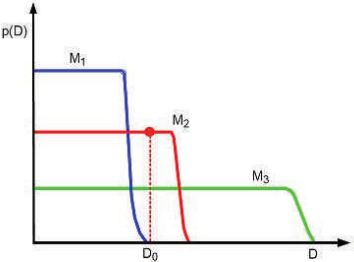
\includegraphics[scale=.80]{Bayesian-Occams-razor.png}
\caption{A schematic illustration of the Bayesian Occam’s razor. The broad (green) curve corresponds to a complex model, the narrow (blue) curve to a simple model, and the middle (red) curve is just right. Based on Figure 3.13 of (Bishop 2006a). }
\label{fig:Bayesian-Occams-razor} 
\end{figure}

When using the Bayesian approach, we are not restricted to evaluating the evidence at a finite grid of values. Instead, we can use numerical optimization to find $\lambda^*=\arg\max_{\lambda}p(\mathcal{D}|\lambda)$. This technique is called \textbf{empirical Bayes} or \textbf{type II maximum likelihood} (see Section \ref{sec:Empirical-Bayes} for details). An example is shown in Figure TODO(b): we see that the curve has a similar shape to the CV estimate, but it can be computed more efficiently.


\subsection{Computing the marginal likelihood (evidence)}
\label{sec:Computing-the-marginal-likelihood}
When discussing parameter inference for a fixed model, we often wrote
\begin{equation}
p(\vec{\theta}|\mathcal{D},m) \propto p(\vec{\theta}|m)p(\mathcal{D}|\vec{\theta},m)
\end{equation}
thus ignoring the normalization constant $p(\mathcal{D}|m)$. This is valid since $p(\mathcal{D}|m)$is constant wrt $\vec{\theta}$. However, when comparing models, we need to know how to compute the marginal likelihood, $p(\mathcal{D}|m)$. In general, this can be quite hard, since we have to integrate over all possible parameter values, but when we have a conjugate prior, it is easy to compute, as we now show.

Let $p(\vec{\theta})=q(\vec{\theta})/Z_0$ be our prior, where $q(\vec{\theta})$ is an unnormalized distribution, and $Z_0$ is the normalization constant of the prior. Let $p(\mathcal{D}|\vec{\theta})=q(\mathcal{D}|\vec{\theta})/Z_{\ell}$ be the likelihood, where $Z_{\ell}$ contains any constant factors in the likelihood. Finally let $p(\vec{\theta}|\mathcal{D})=q(\vec{\theta}|\mathcal{D})/Z_N$ be our posterior , where $q(\vec{\theta}|\mathcal{D})=q(\mathcal{D}|\vec{\theta})q(\vec{\theta})$ is the unnormalized posterior, and $Z_N$ is the normalization constant of the posterior. We have
\begin{align}
p(\vec{\theta}|\mathcal{D})& =\dfrac{p(\mathcal{D}|\vec{\theta})p(\vec{\theta})}{p(\mathcal{D})} \\
\dfrac{q(\vec{\theta}|\mathcal{D})}{Z_N}& =\dfrac{q(\mathcal{D}|\vec{\theta})q(\vec{\theta})}{Z_{\ell}Z_0p(\mathcal{D})} \\
p(\mathcal{D})& = \dfrac{Z_N}{Z_0Z_{\ell}}
\end{align}

So assuming the relevant normalization constants are tractable, we have an easy way to compute the marginal likelihood. We give some examples below.

\subsubsection{Beta-binomial model}
Let us apply the above result to the Beta-binomial model. Since we know $p(\vec{\theta}|\mathcal{D})=\mathrm{Beta}(\vec{\theta}|a',b')$, where $a'=a+N_1$, $b'=b+N_0$, we know the normalization constant of the posterior is $B(a',b')$. Hence
\begin{align}
p(\theta|\mathcal{D})& =\dfrac{p(\mathcal{D}|\theta)p(\theta)}{p(\mathcal{D})} \\
    & =\dfrac{1}{p(\mathcal{D})}\left[\dfrac{1}{B(a,b)}\theta^{a-1}(1-\theta)^{b-1}\right] \nonumber \\
	& \quad \left[\dbinom{N}{N_1}\theta^{N_1}(1-\theta)^{N_0}\right] \\
	& =\dbinom{N}{N_1}\dfrac{1}{p(\mathcal{D})}\dfrac{1}{B(a,b)}\left[\theta^{a+N_1-1}(1-\theta)^{b+N_0-1}\right]
\end{align}

So
\begin{align}
\dfrac{1}{B(a+N_1,b+N_0)} & = \dbinom{N}{N_1}\dfrac{1}{p(\mathcal{D})}\dfrac{1}{B(a,b)} \\
p(\mathcal{D}) & = \dbinom{N}{N_1}\dfrac{B(a+N_1,b+N_0)}{B(a,b)}
\end{align}

The marginal likelihood for the Beta-Bernoulli model is the same as above, except it is missingthe $\binom{N}{N_1}$ term.

\subsubsection{Dirichlet-multinoulli model}
By the same reasoning as the Beta-Bernoulli case, one can show that the marginal likelihood for the Dirichlet-multinoulli model is given by
\begin{align}
p(\mathcal{D}) & =\dfrac{B(\vec{N}+\vec{\alpha})}{B(\vec{\alpha})} \\
   & = \dfrac{\Gamma(\sum_k \alpha_k)}{\Gamma(N+\sum_k \alpha_k)}\prod\limits_k \dfrac{\Gamma(N_k+\alpha_k)}{\Gamma(\alpha_k)}
\end{align}

\subsubsection{Gaussian-Gaussian-Wishart model}
Consider the case of an MVN with a conjugate NIW prior. Let $Z_0$ be the normalizer for the prior, $Z_N$ be normalizer for the posterior, and let $Z_{\ell}(2\pi)^{ND/2}=$ be the normalizer for the likelihood. Then it is easy to see that
\begin{align}
p(\mathcal{D})& =\dfrac{Z_N}{Z_0Z_{\ell}} \\
   & = \dfrac{1}{(2\pi)^{ND/2}}\dfrac{\left(\frac{2\pi}{\kappa_N}\right)^{D/2}|\vec{S}_N|^{-\nu_N/2}2^{(\nu_0+N)D/2}\Gamma_D(\nu_N/2)}{\left(\frac{2\pi}{\kappa_0}\right)^{D/2}|\vec{S}_0|^{-\nu_0/2}2^{\nu_0D/2}\Gamma_D(\nu_0/2)} \\
   & = \dfrac{1}{\pi^{ND/2}}\left(\dfrac{\kappa_0}{\kappa_N}\right)^{D/2}\dfrac{|\vec{S}_0|^{\nu_0/2}}{|\vec{S}_N|^{\nu_N/2}}\dfrac{\Gamma_D(\nu_N/2)}{\Gamma_D(\nu_0/2)}
\end{align}

\subsubsection{BIC approximation to log marginal likelihood}
In general, computing the integral in Equation \ref{eqn:marginal-likelihood} can be quite difficult. One simple but popular approximation is known as the \textbf{Bayesian information criterion} or \textbf{BIC}, which has the following form (Schwarz 1978):
\begin{equation}
\mathrm{BIC} \triangleq \log p(\mathcal{D}|\hat{\vec{\theta}})-\dfrac{\mathrm{dof}(\hat{\vec{\theta}})}{2}\log{N}
\end{equation}
where $\mathrm{dof}(\hat{\vec{\theta}})$ is the number of \textbf{degrees of freedom} in the model, and $\hat{\vec{\theta}}$ is the MLE for the model. We see that this has the form of a \textbf{penalized log likelihood}, where the penalty term depends on the model’s complexity. See Section TODO for the derivation of the BIC score.

As an example, consider linear regression. As we show in Section TODO, the MLE is given by $\hat{\vec{w}}=(\vec{X}^T\vec{X})^{-1}\vec{X}^T\vec{y}$ and $\sigma^2=\frac{1}{N}\sum_{i=1}^N (y_i-\hat{\vec{w}}^T\vec{x}_i)$. The corresponding log likelihood is given by
\begin{equation}
\log p(\mathcal{D}|\hat{\vec{\theta}}) = -\dfrac{N}{2}\log(2\pi\hat{\sigma}^2)-\dfrac{N}{2}
\end{equation}

Hence the BIC score is as follows (dropping constant terms)
\begin{equation}
\mathrm{BIC}=-\dfrac{N}{2}\log(\hat{\sigma}^2)-\dfrac{D}{2}\log{N}
\end{equation}
where $D$ is the number of variables in the model. In the statistics literature, it is common to use an alternative definition of BIC, which we call the BIC \emph{cost}(since we want to minimize it):
\begin{equation}
\mathrm{BIC\text{-}cost} \triangleq -2\log p(\mathcal{D}|\hat{\vec{\theta}})-\mathrm{dof}(\hat{\vec{\theta}})\log{N} \approx -2\log{p(\mathcal{D})}
\end{equation}

In the context of linear regression, this becomes
\begin{equation}
\mathrm{BIC\text{-}cost} = N\log(\hat{\sigma}^2)+D\log{N}
\end{equation}

The BIC method is very closely related to the \textbf{minimum description length} or \textbf{MDL} principle, which characterizes the score for a model in terms of how well it fits the data, minus how complex the model is to define. See (Hansen and Yu 2001) for details.

There is a very similar expression to BIC/ MDL called the \textbf{Akaike information criterion} or \textbf{AIC}, defined as
\begin{equation}
\mathrm{AIC}(m,\mathcal{D}) = \log{p(\mathcal{D}|\hat{\vec{\theta}}_{MLE})}-\mathrm{dof}(m)
\end{equation}

This is derived from a frequentist framework, and cannot be interpreted as an approximation to the marginal likelihood. Nevertheless, the form of this expression is very similar to BIC. We see that the penalty for AIC is less than for BIC. This causes AIC to pick more complex models. However, this can result in better predictive accuracy. See e.g., (Clarke et al. 2009, sec 10.2) for further discussion on such information criteria.

\subsubsection{Effect of the prior}
Sometimes it is not clear how to set the prior. When we are performing posterior inference, the details of the prior may not matter too much, since the likelihood often overwhelms the prior anyway. But when computing the marginal likelihood, the prior plays a much more important role, since we are averaging the likelihood over all possible parameter settings, as weighted by the prior.

If the prior is unknown, the correct Bayesian procedure is to put a prior on the prior. If the prior is unknown, the correct Bayesian procedure is to put a prior on the prior. 


\subsection{Bayes factors}
Suppose our prior on models is uniform, $p(m) \propto 1$. Then model selection is equivalent to picking the model with the highest marginal likelihood. Now suppose we just have two models we are considering, call them the \textbf{null hypothesis}, $M_0$, and the \textbf{alternative hypothesis}, $M_1$. Define the \textbf{Bayes factor} as the ratio of marginal likelihoods:
\begin{equation}
\mathrm{BF}_{1,0} \triangleq \dfrac{p(\mathcal{D}|M_1)}{p(\mathcal{D}|M_0)}=\dfrac{p(M_1|\mathcal{D})}{p(M_2|\mathcal{D})}/\dfrac{p(M_1)}{p(M_0)}
\end{equation}


\section{Priors}
The most controversial aspect of Bayesian statistics is its reliance on priors. Bayesians argue this is unavoidable, since nobody is a \textbf{tabula rasa} or \textbf{blank slate}: all inference must be done conditional on certain assumptions about the world. Nevertheless, one might be interested in minimizing the impact of one’s prior assumptions. We briefly discuss some ways to do this below.


\subsection{Uninformative priors}
If we don’t have strong beliefs about what $\theta$ should be, it is common to use an \textbf{uninformative} or \textbf{non-informative} prior, and to “let the data speak for itself”.


\subsection{Robust priors}
In many cases, we are not very confident in our prior, so we want to make sure it does not have an undue influence on the result. This can be done by using \textbf{robust priors}(Insua and Ruggeri 2000), which typically have heavy tails, which avoids forcing things to be too close to the prior mean.


\subsection{Mixtures of conjugate priors}
Robust priors are useful, but can be computationally expensive to use. Conjugate priors simplify the computation, but are often not robust, and not flexible enough to encode our prior knowledge. However, it turns out that a \textbf{mixture of conjugate priors} is also conjugate, and can approximate any kind of prior (Dallal and Hall 1983; Diaconis and Ylvisaker 1985). Thus such priors provide a good compromise between computational convenience and flexibility.


\section{Hierarchical Bayes}
A key requirement for computing the posterior $p(\vec{\theta}|\mathcal{D})$ is the specification of a prior $p(\vec{\theta}|\vec{\eta})$, where $\vec{\eta}$ are the hyper-parameters. What if we don’t know how to set $\vec{\eta}$? In some cases, we can use uninformative priors, we we discussed above. A more Bayesian approach is to put a prior on our priors! In terms of graphical models (Chapter TODO), we can represent the situation as follows:
\begin{equation}
\vec{\eta} \rightarrow \vec{\theta} \rightarrow \mathcal{D}
\end{equation}

This is an example of a \textbf{hierarchical Bayesian model}, also called a \textbf{multi-level} model, since there are multiple levels of unknown quantities. 


\section{Empirical Bayes}
\label{sec:Empirical-Bayes}

\begin{table}
\normalsize	
\centering
\begin{tabular}{ll}
\hline\noalign{\smallskip}
\textbf{Method} & \textbf{Definition} \\
\noalign{\smallskip}\svhline\noalign{\smallskip}
Maximum likelihood & $\hat{\vec{\theta}}=\arg\max_{\vec{\theta}} p(\mathcal{D}|\vec{\theta})$ \\
MAP estimation & $\hat{\vec{\theta}}=\arg\max_{\vec{\theta}} p(\mathcal{D}|\vec{\theta})p(\vec{\theta}|\vec{\eta})$ \\
\multirow{2}{*}{ML-II (\textbf{Empirical Bayes})} & $\hat{\vec{\eta}}=\arg\max_{\vec{\eta}} \int p(\mathcal{D}|\vec{\theta})p(\vec{\theta}|\vec{\eta})\mathrm{d}\vec{\theta}$ \\
                                                  & $\quad =\arg\max_{\vec{\eta}}p(\mathcal{D}|\vec{\eta})$ \\
\multirow{2}{*}{MAP-II} & $\hat{\vec{\eta}}=\arg\max_{\vec{\eta}} \int p(\mathcal{D}|\vec{\theta})p(\vec{\theta}|\vec{\eta})p(\vec{\eta})\mathrm{d}\vec{\theta}$ \\
                        & $\quad =\arg\max_{\vec{\eta}}p(\mathcal{D}|\vec{\eta})p(\vec{\eta})$ \\
Full Bayes & $p(\vec{\theta},\vec{\eta}|\mathcal{D}) \propto p(\mathcal{D}|\vec{\theta})p(\vec{\theta}|\vec{\eta})$ \\
\noalign{\smallskip}\hline
\end{tabular}
\end{table}


\section{Bayesian decision theory}
\label{sec:Bayesian-decision-theory}
We have seen how probability theory can be used to represent and updates our beliefs about the state of the world. However, ultimately our goal is to convert our beliefs into actions. In this section, we discuss the optimal way to do this.

Our goal is to devise a \textbf{decision procedure} or \textbf{policy}, $f(\vec{x}) : \mathcal{X} \rightarrow \mathcal{Y}$, which minimizes the \textbf{expected loss} $R_{\mathrm{exp}}(f)$(see Equation \ref{eqn:expected-loss}).

In the Bayesian approach to decision theory, the optimal output, having observed $\vec{x}$, is defined as the output $a$ that minimizes the \textbf{posterior expected loss}:
\begin{equation}
\rho(f)=\mathbb{E}_{p(y|\vec{x})}[L(y,f(\vec{x}))]=\begin{cases}
\sum\limits_y L[y,f(\vec{x})]p(y|\vec{x}) \\
\int\limits_y L[y,f(\vec{x})]p(y|\vec{x})\mathrm{d}y
\end{cases}
\end{equation}

Hence the \textbf{Bayes estimator}, also called the \textbf{Bayes decision rule}, is given by
\begin{equation}
\delta(\vec{x})=\arg\min\limits_{f \in \mathcal{H}} \rho(f)
\end{equation}


\subsection{Bayes estimators for common loss functions}


\subsubsection{MAP estimate minimizes 0-1 loss}
When $L(y,f(x))$ is \textbf{0-1 loss}(Section \ref{sec:Loss-function-and-risk-function}), we can proof that MAP estimate minimizes 0-1 loss, 
\begin{align*}
\arg\min\limits_{f \in \mathcal{H}} \rho(f)& =\arg\min\limits_{f \in \mathcal{H}} \sum\limits_{i=1}^K{L[C_k,f(\vec{x})]p(C_k|\vec{x})} \\
         & =\arg\min\limits_{f \in \mathcal{H}} \sum\limits_{i=1}^K{\mathbb{I}(f(\vec{x}) \neq C_k)p(C_k|\vec{x})} \\
		 & =\arg\min\limits_{f \in \mathcal{H}} \sum\limits_{i=1}^K{p(f(\vec{x}) \neq C_k|\vec{x})} \\
		 & =\arg\min\limits_{f \in \mathcal{H}} \left[1-{p(f(\vec{x}) = C_k|\vec{x})}\right] \\
		 & =\arg\max\limits_{f \in \mathcal{H}} p(f(\vec{x}) = C_k|\vec{x})
\end{align*}


\subsubsection{Posterior mean minimizes	$\ell_2$(quadratic) loss}
For continuous parameters, a more appropriate loss function is \textbf{squared error}, \textbf{$\ell_2$ loss}, or \textbf{quadratic loss}, defined as $L(y,f(\vec{x}))=\left[y-f(\vec{x})\right]^2$.

The posterior expected loss is given by
\begin{equation}\begin{split}
\rho(f) & =\int\limits_y L[y,f(\vec{x})]p(y|\vec{x})\mathrm{d}y \\
        & =\int\limits_y \left[y-f(\vec{x})\right]^2p(y|\vec{x})\mathrm{d}y \\
        & =\int\limits_y \left[y^2-2yf(\vec{x})+f(\vec{x})^2\right]p(y|\vec{x})\mathrm{d}y
\end{split}\end{equation}

Hence the optimal estimate is the posterior mean:
\begin{align}
& \dfrac{\partial \rho}{\partial f} =\int\limits_y [-2y+2f(\vec{x})]p(y|\vec{x})\mathrm{d}y=0 \Rightarrow \nonumber \\
& \int\limits_y f(\vec{x})p(y|\vec{x})\mathrm{d}y = \int\limits_y yp(y|\vec{x})\mathrm{d}y \nonumber \\
& f(\vec{x}) \int\limits_y p(y|\vec{x})\mathrm{d}y = \mathbb{E}_{p(y|\vec{x})}[y] \nonumber \\
& f(\vec{x}) = \mathbb{E}_{p(y|\vec{x})}[y]
\end{align}

This is often called the \textbf{minimum mean squared error} estimate or \textbf{MMSE} estimate.


\subsubsection{Posterior median minimizes $\ell_1$(absolute) loss}
The $\ell_2$ loss penalizes deviations from the truth quadratically, and thus is sensitive to outliers. A more robust alternative is the absolute or $\ell_1$ loss. The optimal estimate is the posterior median, i.e., a value $a$ such that $P(y<a|\vec{x})=P(y \geq a|\vec{x})=0.5$.

\begin{proof}
\begin{align*}
\rho(f)& =\int\limits_y L[y,f(\vec{x})]p(y|\vec{x})\mathrm{d}y=\int\limits_y |y-f(\vec{x})|p(y|\vec{x})\mathrm{d}y \\
       & =\int\limits_y [f(\vec{x})-y]p(y<f(\vec{x})|\vec{x})+ \\
	   & \quad [y-f(\vec{x})]p(y \geq f(\vec{x})|\vec{x})\mathrm{d}y \\
& \dfrac{\partial \rho}{\partial f}=\int\limits_y \left[p(y<f(\vec{x})|\vec{x})-p(y \geq f(\vec{x})|\vec{x})\right]\mathrm{d}y=0 \Rightarrow \\
& p(y<f(\vec{x})|\vec{x})=p(y \geq f(\vec{x})|\vec{x})=0.5 \\
& \therefore f(\vec{x})=\text{median}
\end{align*}
\end{proof}


\subsubsection{Reject option}
In classification problems where $p(y|\vec{x})$ is very uncertain, we may prefer to choose a reject action, in which we refuse to classify the example as any of the specified classes, and instead say “don’t know”. Such ambiguous cases can be handled by e.g., a human expert. This is useful in \textbf{risk averse} domains such as medicine and finance.

We can formalize the reject option as follows. Let choosing $f(\vec{x})=c_{K+1}$ correspond to picking the reject action, and choosing $f(\vec{x}) \in \{C_1,...,C_k\}$ correspond to picking one of the classes. Suppose we define the loss function as
\begin{equation}
L(f(\vec{x}), y)=\begin{cases} 
0 & \text{if } f(\vec{x})=y \text{ and } f(\vec{x}),y \in \{C_1,...,C_k\} \\
\lambda_s & \text{if } f(\vec{x}) \neq y \text{ and } f(\vec{x}),y \in \{C_1,...,C_k\} \\
\lambda_r & \text{if } f(\vec{x})=C_{K+1}
\end{cases}
\end{equation}
where $\lambda_s$ is the cost of a substitution error, and $\lambda_r$ is the cost of the reject action. 


\subsubsection{Supervised learning}
We can define the loss incurred by $f(\vec{x})$ (i.e., using this predictor) when the unknown state of nature is $\vec{\theta}$(the parameters of the data generating mechanism) as follows:
\begin{equation}
L(\vec{\theta},f) \triangleq \mathbb{E}_{p(\vec{x},y|\vec{\theta})}[\ell(y-f(\vec{x}))]
\end{equation}

This is known as the \textbf{generalization error}. Our goal is to minimize the posterior expected loss, given by
\begin{equation}
\rho(f|\mathcal{D}) = \int{p(\vec{\theta}|\mathcal{D})L(\vec{\theta},f)}\mathrm{d}\vec{\theta}
\end{equation}

This should be contrasted with the frequentist risk which is defined in Equation TODO.


\subsection{The false positive vs false negative tradeoff}
In this section, we focus on binary decision problems, such as hypothesis testing, two-class classification, object/ event detection, etc. There are two types of error we can make: a \textbf{false positive}(aka \textbf{false alarm}), or a \textbf{false negative}(aka \textbf{missed detection}). The 0-1 loss treats these two kinds of errors equivalently. However, we can consider the following more general loss matrix:

TODO

%\chapter{Frequentist statistics}
\label{Frequentist Statistics}

Attempts have been made to devise approaches to statistical inference that avoid treating parameters like random variables, and which thus avoid the use of priors and Bayes rule. Such approaches are known as \textbf{frequentist statistics}, \textbf{classical statistics} or \textbf{orthodox statistics}. Instead of being based on the posterior distribution, they are based on the concept of a sampling distribution.


\section{Sampling distribution of an estimator}
In frequentist statistics, a parameter estimate $\hat{\vec{\theta}}$ is computed by applying an \textbf{estimator} $\delta$ to some data $\mathcal{D}$, so $\hat{\vec{\theta}}=\delta(\mathcal{D})$. The parameter is viewed as fixed and the data as random, which is the exact opposite of the Bayesian approach. The uncertainty in the parameter estimate can be measured by computing the \textbf{sampling distribution} of the estimator. To understand this


\subsection{Bootstrap}
We might think of the bootstrap distribution as a “poor man’s” Bayes posterior, see (Hastie et al. 2001, p235) for details.


\subsection{Large sample theory for the MLE *}



\section{Frequentist decision theory}
In frequentist or classical decision theory, there is a loss function and a likelihood, but there is no prior and hence no posterior or posterior expected loss. Thus there is no automatic way of deriving an optimal estimator, unlike the Bayesian case. Instead, in the frequentist approach, we are free to choose any estimator or decision procedure $f: \mathcal{X} \rightarrow \mathcal{Y}$ we want.

Having chosen an estimator, we define its expected loss or \textbf{risk} as follows:
\begin{equation}\begin{split}
R_{\mathrm{exp}}(\theta,f) & \triangleq \mathbb{E}_{p(\tilde{\mathcal{D}}|\theta^*)}[L(\theta^*, f(\tilde{\mathcal{D}}))] \\
    & =\int L(\theta^*, f(\tilde{\mathcal{D}}))p(\tilde{\mathcal{D}}|\theta^*)\mathrm{d}\tilde{\mathcal{D}}
\end{split}\end{equation}
where˜$\tilde{\mathcal{D}}$ is data sampled from “nature’s distribution”, which is represented by parameter $\theta^*$. In other words, the expectation is wrt the sampling distribution of the estimator. Compare this to the Bayesian posterior expected loss:
\begin{equation}
\rho(f|\mathcal{D},)
\end{equation}


\section{Desirable properties of estimators}


\section{Empirical risk minimization}


\subsection{Regularized risk minimization}


\subsection{Structural risk minimization}


\subsection{Estimating the risk using cross validation}


\subsection{Upper bounding the risk using statistical learning theory *}


\subsection{Surrogate loss functions}
\label{sec:Surrogate-loss-functions}

\textbf{log-loss}
\begin{equation}\label{eqn:log-loss}
L_{\mathrm{nll}}(y,\eta)=-\log p(y|\vec{x},\vec{w})=\log(1+e^{-y\eta})
\end{equation}


\section{Pathologies of frequentist statistics *}


\chapter{Linear Regression}


\section{Introduction}
Linear regression is the “work horse” of statistics and (supervised) machine learning. When augmented with kernels or other forms of basis function expansion, it can model also nonlinear relationships. And when the Gaussian output is replaced with a Bernoulli or multinoulli distribution, it can be used for classification, as we will see below. So it pays to study this model in detail.

In the simplest approach,we can directly construct an appropriate function $y(\vec{x})$ whose values for new inputs $\vec{x}$ constitute the predictions for the corresponding values of $t$.More generally,from a probabilistic perspective,we aim to model the predictive distribution $p(t|x)$ because this expresses the uncertainty about the value of $t$ for each value of $x$.

\section{Representation}
The simplest linear model for regression is \textbf{linear regression} that involves a linear combination of the input variables
\begin{equation}
y(\vec{x},\vec{w}) = w_0+w_1x_1+...+w_Dx_D
\end{equation}
where $\vec{x}=(x_1,...,x_D)^T$.

Linear regression can be made to model non-linear relationships by replacing $\vec{x}$ with some non-linear function of the inputs, $\phi(\vec{x})$.Consider the linear combinations of fixed nonlinear functions of the input variables,of the form
\begin{equation}
y(\vec{x},\vec{w}) = w_0+\sum_{j=1}^{M-1}w_j\phi_j(x) 
=\sum_{j=0}^{M-1}w_j\phi_j(x) = \vec{w}^T\phi(x)
\end{equation}
where $\phi_j(x)$ are known as \textbf{basis functions},
$\vec{w}=(w_0,...,w_{M-1})^T$ and $\phi=(\phi_0,...,\phi_{M-1})^T$.
This is known as \textbf{basis function expansion}. (Note that the model is still linear in the parameters $\vec{w}$, so it is still called linear regression; the importance of this will become clear below.) A simple example are polynomial basis functions, where the model has the form
\begin{equation}
\phi(x)=(1, x, \cdots, x^d)
\end{equation}


As before,we assume that the target variable is given by a deterministic function $y(\vec{x},\vec{w})$ with additive Gaussian noise so that
\begin{equation}
t=y(\vec{x},\vec{w})+\epsilon
\end{equation}
where $\epsilon$ is a zero mean Gaussian random variable with precision(inverse variance) $\beta$.Thus
\begin{equation}\label{eqn:linear regression representation}
p(t|\vec{x},\vec{w},\beta)=\mathcal{N}(t|h(\vec{x},\vec{w}),\beta^{-1})
\end{equation}
or 
\begin{eqnarray}
& y(\vec{x}) = \vec{w}^T\vec{x}+\epsilon \\
& p(y|\vec{x},\vec{\theta})=\mathcal{N}(y|\vec{w}^T\vec{x}, \sigma^2) \\
\end{eqnarray}
where $\vec{w}$ (\textbf{weight vector}) and $\vec{x}$ are extended vectors, $\vec{x}=(1,x)$, $\vec{w}=(b,w)$ and $\epsilon$ has a \textbf{Gaussian} or \textbf{normal} distribution.$w_0$ is the intercept or \textbf{text}

 
%\begin{eqnarray}
%& y(\vec{x}) = \vec{w}^T\phi(\vec{x})+\epsilon \\
%& p(y|\vec{x},\vec{\theta})=\mathcal{N}(y|\vec{w}^T\phi(\vec{x}), \sigma^2)
%\end{eqnarray}


\section{Maximum likelihood estimations(least squares)}
Assume the training examples are \textbf{independently and identically distributed(IID)},we obtain the \textbf{likelihood function},which is a function of adjustable parameters $\vec{w}$ and $\beta$,in the form
\begin{align}\label{eqn:linear regression likelihood}
p(\vec{t}|\vec{X},\vec{w},\beta) =
\prod_{n=1}^{N}\mathcal{N}(t_n|\vec{w}^T\phi(\vec{x_n}),\beta^{-1})
\end{align}
we can write the \textbf{log-likelihood} (logarithm of the likelihood) function as follows:
\begin{equation}
\ell(\vec{\theta}) \triangleq \log p(\mathcal{D}|\vec{\theta})
\end{equation}
A common way to estimate the parameters of a statistical model is to compute the MLE(Maximum likelihood estimations),which is defined as
\begin{equation}
\vec{\hat{\theta}}=\arg\max_\theta{\log p(\mathcal{D}|\vec{\theta})}
\end{equation}

Instead of maximizing the log-likelihood, we can equivalently minimize the \textbf{negative log likelihood} or \textbf{NLL}:
\begin{equation}
\text{NLL}(\vec{\theta}) \triangleq -\ell(\vec{\theta})=-\log p(\mathcal{D}|\vec{\theta})
\end{equation}

The NLL formulation is sometimes more convenient, since many optimization software packages are designed to find the minima of functions, rather than maxima.

Now let us apply the method of MLE to the linear regression setting. Inserting the definition of the Gaussian into the above, we find that the log likelihood is given by
\begin{align}
\ell(\vec{\theta}) &= \log p(\vec{T}|\vec{w},\beta) \\
&=\sum_{n=1}^{N}\log \mathcal{N}(t_n|\vec{w}^T\phi(\vec{x_n}),\beta^{-1}) \\
&=\sum\limits_{i=1}^N \log\left[\dfrac{1}{\sqrt{2\pi}\sigma}\exp\left(-\dfrac{1}{2\sigma^2}(y_i-\vec{w}^T\vec{x}_i)^2\right)\right] \\
&=\dfrac{N}{2}\log \beta-\dfrac{N}{2}\log (2\pi)-\beta E_D(\vec{w}) \\
&=-\dfrac{1}{2\sigma^2}\text{RSS}(\vec{w})-\dfrac{\vec{w}}{2}\log(2\pi\sigma^2)
\end{align}
where the sum-of-squares error function is defined by
\begin{equation}
E_D(\vec{w}) =
\dfrac{1}{2}\sum_{n=1}^{N}\{t_n-\vec{w}^T\phi(\vec{x_n}) \}^2
\end{equation}
RSS stands for \textbf{residual sum of squares} and is defined by
\begin{equation}
\text{RSS}(\vec{w}) \triangleq \sum\limits_{i=1}^N (t_i-\vec{w}^T\vec{x}_i)^2
\end{equation}
The RSS can also be written as the square of the $\ell_2$ \textbf{norm} of the vector of residual errors:
\begin{equation}
RSS(\vec{w}) = \parallel\epsilon\parallel_2^2 = \sum_{i=1}^{N}\epsilon_i^2
\end{equation}
where $\epsilon_i = (t_i - \vec{w}^T\vec{x_i})$.

There two ways to compute the optimal solution of likelihood function.

\subsection{Derivations of the MLE}
We see that maximizing the likelihood function under a conditional Gaussian noise distribution for a linear model is equivalent to $\vec{w}$ minimizing the RSS(or $E_D$), so this method is known as \textbf{least squares}.The gradient of the log likelihood function takes the form
\begin{equation}
\nabla\log p(\vec{t}|\vec{w},\beta)
=\sum_{n=1}^{N}\{t_n-\vec{w}^T\phi(\vec{x_n}) \}\phi(\vec{x_n})^T
\end{equation}

Let's drop constants with respect to $\vec{w}$ and NLL can be written as
\begin{equation}
\text{NLL}(\vec{w}) = \dfrac{1}{2}\sum\limits_{i=1}^N (y_i-\vec{w}^T\vec{\phi}_i)^2
\end{equation}

Define $\vec{y}=(t_1,t_2,\cdots,t_N)$, $\vec{\Phi}=\left(\begin{array}{c}\vec{\phi}_1^T \\ \vec{\phi}_2^T \\ \vdots \\ \vec{\phi}_N^T\end{array}\right)$, then we can rewritten the objective in a form that is more amendable to differentiation:
\begin{align}
\text{NLL}(\vec{w}) &= \dfrac{1}{2}(\vec{t}-\vec{\Phi}\vec{w})^T(\vec{t}-\vec{\Phi}\vec{w})\\
&= \dfrac{1}{2} [\vec{w^T} (\vec{\Phi}^T\vec{\Phi})\vec{w} - \vec{t}^T\vec{\Phi}\vec{w}- \vec{w}^T\vec{x}^T\vec{t}  +\vec{t}^T\vec{t}]			\\
\Rightarrow
\dfrac{\partial}{\partial \vec{w}}\text{NLL} &= \dfrac{1}{2} \vec{w^T} (\vec{\Phi}^T\vec{\Phi})\vec{w} -\vec{w}^T(\vec{\Phi}^T\vec{t}) 
\end{align}

where
$\begin{cases}
\vec{\Phi} = \begin{bmatrix}
&\vec{\Phi_1^T} \\
&\vec{\Phi_2^T} \\
& ... \\
&\vec{\Phi_n^T}
\end{bmatrix} \\	
\vec{\Phi^T}\vec{\Phi} =
\begin{bmatrix}
\vec{\Phi_1} & \vec{\Phi_2} & ...&\vec{\Phi_n}
\end{bmatrix} 
\cdot
\begin{bmatrix}
&\vec{\Phi_1^T} \\
&\vec{\Phi_2^T} \\
& ... \\
&\vec{\Phi_N^T}
\end{bmatrix}  = \sum\limits_{i=1}^{N}\vec{\phi_i}\vec{\phi_i^T} = \textbf{sum of squares matrix} \\
\end{cases}$

Note that $\vec{\Phi}$ is an $N\times M$ matrix,called the \textbf{design matrix},whose elements are given by $\Phi_{nj}=\phi_j(\vec{x_n})$ so that
\begin{equation}
\vec{\Phi}=
\begin{bmatrix}
\phi_0(\vec{x_1}) &	\phi_1(\vec{x_1}) &...&\phi_{M-1}(\vec{x_1}) \\
\phi_0(\vec{x_2}) & \phi_1(\vec{x_2}) &...&\phi_{M-1}(\vec{x_2}) \\
\vdots &\vdots &\vdots&\vdots \\
\phi_0(\vec{x_N})& \phi_1(\vec{x_{N}})& \cdot &\phi_{M-1}(\vec{x_N})\\
\end{bmatrix}
\end{equation}



When $\mathcal{D}$ is small(for example, $N < 1000$), we can use the following equation to compute $\vec{w}$ directly
\begin{equation}
\vec{w}_{ML}=\hat{\vec{w}}_{\mathrm{OLS}}=(\vec{\Phi}^T\vec{\Phi})^{-1}\vec{\Phi}^T\vec{t}
\end{equation}

The corresponding solution $\hat{\vec{w}}_{\mathrm{OLS}}$ to this linear system of equations is called the \textbf{ordinary least squares} or \textbf{OLS} or \textbf{normal equation} solution.

\begin{proof}
We now state without proof some facts of matrix derivatives (we won’t need all of these at this section).
\begin{eqnarray}
trA &\triangleq& \sum\limits_{i=1}^n A_{ii} \nonumber \\
\frac{\partial}{\partial A}AB &=& B^T \\
\frac{\partial}{\partial A^T}f(A) &=& \left[\frac{\partial}{\partial A}f(A)\right]^T \label{eqn:matrix-1} \\
\frac{\partial}{\partial A}ABA^TC &=& CAB+C^TAB^T \label{eqn:matrix-2} \\
\frac{\partial}{\partial A}|A| &=& |A|(A^{-1})^T
\end{eqnarray}

Then,
\begin{eqnarray*}
\text{NLL}(\vec{w}) &=& \frac{1}{2N}(\vec{X}\vec{w}-\vec{y})^T(\vec{X}\vec{w}-\vec{y}) \\
\frac{\partial \text{NLL}}{\partial\vec{w}} 
&=& \frac{1}{2} \frac{\partial}{\partial\vec{w}} (\vec{w}^T\vec{X}^T\vec{X}\vec{w}-\vec{w}^T\vec{X}^T\vec{y}-\vec{y}^T\vec{X}\vec{w}+\vec{y}^T\vec{y}) \\
&=& \frac{1}{2} \frac{\partial}{\partial\vec{w}} (\vec{w}^T\vec{X}^T\vec{X}\vec{w}-\vec{w}^T\vec{X}^T\vec{y}-\vec{y}^T\vec{X}\vec{w}) \\
&=& \frac{1}{2} \frac{\partial}{\partial\vec{w}}  \\
&=& \frac{1}{2} \frac{\partial}{\partial\vec{w}} (tr\vec{w}^T\vec{X}^T\vec{X}\vec{w}-2tr\vec{y}^T\vec{X}\vec{w})
\end{eqnarray*}

Combining Equations \ref{eqn:matrix-1} and \ref{eqn:matrix-2}, we find that 
\begin{equation*}
\frac{\partial}{\partial A^T}ABA^TC = B^TA^TC^T+BA^TC
\end{equation*}

Let $A^T=\vec{w}, B=B^T=\vec{X}^T\vec{X}$, and $C=I$, Hence,
\begin{eqnarray}
\frac{\partial \text{NLL}}{\partial\vec{w}} &=& \frac{1}{2} (\vec{X}^T\vec{X}\vec{w}+\vec{X}^T\vec{X}\vec{w} -2\vec{X}^T\vec{y}) \nonumber \\
						   &=& \frac{1}{2} (\vec{X}^T\vec{X}\vec{w} - \vec{X}^T\vec{y}) \nonumber \\
\frac{\partial \text{NLL}}{\partial\vec{w}} &=& 0 \Rightarrow \vec{X}^T\vec{X}\vec{w} - \vec{X}^T\vec{y} =0 \nonumber \\
\vec{X}^T\vec{X}\vec{w} &=& \vec{X}^T\vec{y} \label{eqn:normal-equation} \\
\hat{\vec{w}}_{\mathrm{OLS}} &=& (\vec{X}^T\vec{X})^{-1}\vec{X}^T\vec{y} \nonumber
\end{eqnarray}
\end{proof}
Equation \ref{eqn:normal-equation} is known as the \textbf{normal equation}.
\begin{proof}
Consider $\mathbf{vector-vector}$ differentiation,if $\mathbf{A}$ is not a function of $\vec{x}$ then
\begin{equation}
\dfrac{\partial\vec{X}^TA\vec{X}}{\partial\vec{X}} = \vec{X}^T(\mathbf{A}+\mathbf{A}^T) = (\mathbf{A}+\mathbf{A}^T)\vec{X}
\end{equation}
\end{proof}
Then,we can derivate $\dfrac{\partial NLL}{\partial \vec{w}}$
\begin{eqnarray}
g(\vec{w}) &= \dfrac{\partial NLL}{\partial\vec{w}} \\
&=\vec{\Phi}^T\vec{\Phi}\vec{w} - \vec{\Phi}^T\vec{y}			
\end{eqnarray}
Setting the derivative to zero,we get
\begin{equation}
	\vec{w} = (\vec{X}^T\vec{X})^{-1}\vec{x}^T\vec{y}
\end{equation}

\subsection{Geometric interpretation}

See Figure \ref{fig:graphical-interpretation-of-OLS}.
\begin{figure}[hbtp]
\centering
    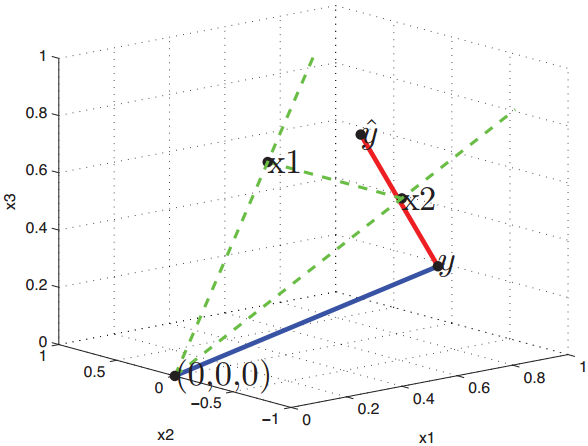
\includegraphics[scale=.50]{graphical-interpretation-of-OLS.png}
\caption{Graphical interpretation of least squares for $N=3$ examples and $D=2$ features. $\tilde{\vec{x}}_1$ and $\tilde{\vec{x}}_2$˜ are vectors in $\mathbb{R}^3$; together they define a 2D plane. $\vec{y}$ is also a vector in $\mathbb{R}^3$ but does not lie on this 2D plane. The orthogonal projection of $\vec{y}$ onto this plane is denoted $\hat{\vec{y}}$. The red line from $\vec{y}$ to $\hat{\vec{y}}$ is the residual, whose norm we want to minimize. For visual clarity, all vectors have been converted to unit norm.}
\label{fig:graphical-interpretation-of-OLS} 
\end{figure}
Given that
\begin{eqnarray}
\vec{X} = \begin{bmatrix}
\vec{x_1}^T &\\
\vec{x_2}^T &\\
 ...        &\\
\vec{x_N}^T
\end{bmatrix} 
= \begin{bmatrix}
\vec{\tilde{x_1}} & \vec{\tilde{x_1}} & ... &\vec{\tilde{x_D}}
\end{bmatrix}\\
\vec{y} = \begin{bmatrix}
t_1 \\
t_2 \\
... \\
t_n
\end{bmatrix} 
\end{eqnarray}
We seek a vector $\hat{\vec{t}} \in \mathbb{R}^N$ that lies in the column linear space of $\vec{X}$ and is as close as possible to $\vec{t}$,i.e.,we want to find
\begin{eqnarray}
\hat{\vec{t}} \in span(\vec{X}) \\
\Rightarrow \hat{\vec{t}} = \vec{X}\vec{w} = w_1\vec{\tilde{x_1}}+\cdot\cdot\cdot+w_D\vec{\tilde{x_D}} \\
\vec{\hat{t}}=\arg\min\limits_{\hat{\vec{t}} \in \text{span} (\{\vec{\tilde{x_1}},...,\vec{\tilde{x_D}}\})}
\end{eqnarray}

To minimize the norm of the residual, $\vec{t}-\hat{\vec{t}}$, we want the residual vector to be orthogonal to every column of $\vec{X}$,so˜ $\tilde{\vec{x}}_j(\vec{t}-\hat{\vec{t}})=0$ for $j=1:D$. Hence
\begin{equation}\begin{split}
\tilde{\vec{x}}_j(\vec{t}-\hat{\vec{t}})=0 & \Rightarrow \vec{X}^T(\vec{t}-\vec{X}\vec{w})=0 \\
                                           & \Rightarrow \vec{w}=(\vec{X}^T\vec{X})^{-1}\vec{X}^T\vec{t}
\end{split}\end{equation}


\subsection{Sequential learning}
Batch techniques,such as the maximum likelihood solution,which involves processing the entire training set in one go(pass),can be computationally costly for large data sets.If the data set is sufficiently large,it may be worthwhile to use \textbf{sequential} algorithms,known as \textbf{on-line} algorithms.
When $\mathcal{D}$ is large, use \textbf{stochastic gradient descent(SGD)},also known as sequential gradient descent.
\begin{align}
E &=\sum_{n}E_n \\
\vec{w}^{\tau+1} &= \vec{w}^{\tau}-\eta\nabla E_n
\end{align}
where $\tau$ denotes the iteration number,the $\eta$ is a learning rate parameter.For the case of sum-of-squares error function,this gives
\begin{equation}
\vec{w}^{\tau+1} = \vec{w}^{\tau}-\eta(t_n-\vec{w}^{(\tau)T}\phi_n)\phi_n
\end{equation}
where $\phi_n=\phi(\vec{x_n})$.This is known as the \textbf{least-mean-squares} or the LMS algorithm.


\begin{align}
\because \dfrac{\partial}{\partial w_i}\text{NLL}(\vec{w})=& \sum\limits_{i=1}^N (\vec{w}^T\vec{x}_i-y_i)x_{ij} \\
\therefore w_j=& w_j - \alpha\dfrac{\partial}{\partial w_j}\text{NLL}(\vec{w}) \nonumber \\
                  =& w_j - \sum\limits_{i=1}^N \alpha(\vec{w}^T\vec{x}_i-y_i)x_{ij} \\
\therefore \vec{w}=& \vec{w}-\alpha(\vec{w}^T\vec{x}_i-y_i)\vec{x}
\end{align}


\section{Ridge regression(MAP)}
One problem with ML estimation is that it can result in over-fitting. In this section, we discuss a way to ameliorate this problem by using MAP estimation with a Gaussian prior.

\subsection{Basic idea}
We can encourage the parameters to be small, thus resulting in a smoother curve, by using a zero-mean Gaussian prior:
\begin{equation}
p(\vec{w})=\prod\limits_j \mathcal{N}(w_j|0,\tau^2)
\end{equation}
where $1/\tau^2$ controls the strength of the prior. The corresponding MAP estimation problem becomes
\begin{equation}
\arg\max_{\vec{w}} \sum\limits_{i=1}^N \log{\mathcal{N}(t_i|w_0+\vec{w}^T\vec{\phi}_i,\sigma^2)}+\sum\limits_{j=1}^D \log{\mathcal{N}(w_j|0,\tau^2)}
\end{equation}

This is equivalent to minimizing the following
\begin{align}\label{eqn:Ridge-regression-J}
J(\vec{w})&=E_D(\vec{w})+\lambda E_W(\vec{w}) \\
&=\dfrac{1}{N}\sum\limits_{i=1}^N (y_i-(w_0+\vec{w}^T\vec{x}_i))^2+\lambda\lVert\vec{w}\rVert^2 , \lambda \triangleq \dfrac{\sigma^2}{\tau^2}
\end{align}
where the first term is the MSE/ NLL as usual, and the second term, $\lambda \geq 0$, is the regularization coefficient that controls the complexity penalty.
Here $E_W(\vec{w})$ is one of the simplest forms of regularizer given by the sum-of-squares of the weight vector elements.
\begin{equation}
E_W(\vec{w})=\dfrac{1}{2}\vec{w}^T\vec{w}
\end{equation}
This particular choice of regularizer is known as \textbf{weight decay}.

The corresponding solution is given by
\begin{equation}\label{eqn:Ridge-regression-solution}
\hat{\vec{w}}_{\mathrm{ridge}}=(\lambda\vec{I}_D+\vec{\Phi}^T\vec{\Phi})^{-1}\vec{\Phi}^T\vec{t}
\end{equation}

This technique is known as \textbf{ridge regression},or \textbf{penalized least squares}. In general, adding a Gaussian prior to the parameters of a model to encourage them to be small is called $\ell_2$ \textbf{regularization} or \textbf{weight decay}. Note that the offset term $w_0$ is not regularized, since this just affects the height of the function, not its complexity.

We will consider a variety of different priors in this book. Each of these corresponds to a different form of \textbf{regularization}. This technique is very widely used to prevent overfitting.

\subsection{Multiple outputs}
Now consider the case where we wish to predict $K>1$ target variables,which we denote collectively by the target vector $\vec{t}$.To use the same set of basis functions to model all the components of the target vector so that
\begin{equation}
\vec{y}(\vec{x},\vec{w}) = \vec{W}^T\phi(x)
\end{equation}
where $\vec{y}$ is a $K$-dimensional column vector,$\vec{W}$ is an $M\times K$ matrix of parameters.

The conditional distribution of the target vector is an isotropic Gaussian
\begin{equation}
p(\vec{t}|\vec{x},\vec{W},\beta) =
\mathcal{N}(\vec{t}|\vec{W}^T\phi(x,\beta^{-1}\vec{I}))
\end{equation}

The log likelihood function is then given by 
\begin{align}
\ln p(\vec{T}|\vec{X},\vec{W},\beta) 
&=\sum_{n=1}^{N}\ln \mathcal{N}(\vec{t_n}|\vec{W}^T\phi(x_n),\beta^{-1}\vec{I}) \\
&=\dfrac{NK}{2}\ln(\dfrac{\beta}{2\pi}) 
 -\dfrac{\beta}{2}\sum_{n=1}^{N}\parallel \vec{t_n}-\vec{W}^T\phi(x_n)\parallel^2
\end{align}
We maximize this function with respect to $\vec{W}$,giving
\begin{equation}
\vec{W}_{ML} = (\vec{\Phi}^T\vec{\Phi})^{-1}\vec{\Phi}^T\vec{T}
\end{equation}


\subsection{Numerically stable computation *}

\begin{equation}\label{eqn:Ridge-regression-SVD}
\hat{\vec{w}}_{\mathrm{ridge}}=\vec{V}(\vec{Z}^T\vec{Z}+\lambda\vec{I}_N)^{-1}\vec{Z}^T\vec{y}
\end{equation}


\subsection{Connection with PCA *}


\subsection{Regularization effects of big data}
Regularization is the most common way to avoid overfitting. However, another effective approach — which is not always available — is to use lots of data. It should be intuitively obvious that the more training data we have, the better we will be able to learn.

In domains with lots of data, simple methods can work surprisingly well (Halevy et al. 2009). However, there are still reasons to study more sophisticated learning methods, because there will always be problems for which we have little data. For example, even in such a data-rich domain as web search, as soon as we want to start personalizing the results, the amount of data available for any given user starts to look small again (relative to the complexity of the problem).

\section{The Bias-Variance Decomposition}
\subsubsection{representation}
Data representation:
N observations of x,wiritten 
$X \equiv (x_1,x_2,...,x_n)^T$
together with corresponding observations of the values of t,denoted 
$t \equiv (t_1,t_2,...t_N)^T$.
\begin{equation}
t_i = f(\vec{x_i}) + \epsilon 
\end{equation}
where the noise $ \epsilon $ has zero mean and variance $ \sigma^2 $.
Find a function \[ \hat{f}(x) \] that approximates the true function \[ t = f(\vec{x}) \] as well as possible.Make "as well as possible" precise  by measuring the mean squared error between y and $ \hat{f}(x) $,we want $ (t - \hat{f}(x))^2 $ to be minimal.
Hypothesis function(model representation):
$y(x,\bold w)= w_0+w_1x+w_2x^2+...+w_Mx^M = \sum_{j=0}^{M}w_jx^j$
M is the order of the polynomial,and $x^j$ denotes $x$ raised to the power of $j$.The polynomial coefficients $w_0,...w_M$ are
collectively denoted by the vector $\mathbf{w}$.

Error Function(Sum of squares of errors between predictions $y(x_n,w)$ for each data point $x_n$ and the corresponding target values $t_n$,so that we minimize:
\begin{equation}
E(\bold w)=\frac{1}{2}\sum_{n=1}^{N}\{y(x_n,\bold w)-t_n \}^2
\end{equation}
root-mean-squre(RMS) error defined by
\begin{equation} 
E_{RMS} = \sqrt[2]{2E(\bold w^*)/N}
\end{equation}
Penalized(regularized) error function
\begin{equation}
\widetilde{E}(\textbf{w}) = \frac{1}{2}\sum_{n=1}^{N}\{y(x_n,\textbf{w}-t_n\}^2 + \frac{1}{2} \parallel \textbf{w} \parallel^2
\end{equation}
where $\parallel \textbf{w} \parallel^2 \equiv \textbf{w}^T\textbf{w}=w_0^2+w_1^2+...+w_M^2$

\subsubsection{Loss function for regression}
\begin{equation}
\mathbb{E}[\mathit{L}] = \iint\mathit{L}(t,y(\textbf{x}))p(\textbf{x},t)d\textbf{x}dt
\end{equation}
A common choice of loss function in squared loss given by 
\begin{eqnarray}
\mathit{L}(t,y(\textbf{x})) = \{y(\textbf{x}) - t\}^2 \\
\mathbb{E}[\mathit{L}] = \iint\{y(\textbf{x}) - t\}^2 p(\textbf{x},t)d\textbf{x}dt.
\end{eqnarray}
Minimize $ \mathbb{E}[\mathit{L}] $ by using the calculus of variations to give 
\begin{equation}
\frac{\delta\mathbb{E}[\mathit{L}]}{\delta y(\mathbf{x}))} = 2 \int\{ y(\mathbf{x} -t) \}p(\mathbf{x},t)dt = 0
\end{equation}
Solving for $ y(\textbf{x}) $ and using the sum and product rules of probability,we obtain
\begin{equation}
y(\textbf{x}) = \frac{\int tp(\textbf{x},t)dt}{p(\textbf{x})} = \int tp(t|\textbf{x})dt = \mathbb{E}[t|\textbf{x}]
\end{equation}

Let's derive this result in a slightly different way.Armed with knowledge that the optimal solution is the 
conditional expectation,we can expand the square term as follows
\begin{equation}
\{y(\textbf{x} -t)\}^2
= \{y(\textbf{x}) - \mathbb{E}[t|\textbf{x}] + \mathbb{E}[t|\textbf{x}] - t )\}^2 
= \{ y(\textbf{x}) - \mathbb{E}[t|\textbf{x}] \}^2 + 2\{ y(\textbf{x}) - \mathbb{E}[t|\textbf{x}] \}\{ \mathbb{E}[t|\textbf{x}]-t \} + \{ \mathbb{E}[t|\textbf{x}] -t \}^2
\end{equation}
where,$ \mathbb{E}[t|\textbf{x}] $ denote $ \mathbb{E}_{t}[t|\textbf{x}] $.Substitute into the loss function and perform the integral over t,we see the cross-term vanishes
\begin{align}\label{eqn:squared loss function}
\mathbb{E}[\mathit{L}]                                                           
&= \iint\{y(\textbf{x}) - t\}^2 p(\textbf{x},t)d\textbf{x}dt                    \\
&= \int \{ y(\textbf{x}) -\mathbb{E}[t|\textbf{x}] \}^2 p(\textbf{x})d\textbf{x} + 
\int\{ \mathbb{E}[t|\textbf{x}] - t \}^2 p(\textbf{x})d\textbf{x}               \\
&= \int \{ y(\textbf{x}) -h(\textbf{x}) \}^2 p(\textbf{x})d\textbf{x} +            
\int\{ h(\textbf{x}) - t \}^2 p(\textbf{x})d\textbf{x}                          \\
&= \int \{ y(\textbf{x}) -h(\textbf{x}) \}^2 p(\textbf{x})d\textbf{x} +            
\int\{ h(\textbf{x}) - t \}^2 p(\textbf{x},t)d\textbf{x}dt                      \\
\end{align}

\subsubsection{Decomposition}
For a popular choice,we use squared loss function,for which the optimal prediction is given by the conditional
expectation,which we denote by h(\textbf{x}) and which is given by 
\begin{equation}
h(\textbf{x}) = \mathbb{E}[t|\textbf{x}] = \int tp(t|\textbf{x})dt
\end{equation}

Consider the integrand of the first term of \ref{eqn:squared loss function},which for particular data set D takes the form
\begin{equation}
\{ y(\textbf{x};D) - h(\textbf{x}) \} ^2
\end{equation}
This quantity will be dependent on the particular data set D,so we take its average over the ensemble of data sets.
If we add and subtract the quantity $ \mathbb{E_D}[y(\textbf{x};D)] $ inside the braces,and then expand,we obtain
\begin{align}
\{ y(\textbf{x};D) - h(\textbf{x}) \} ^2 \\
=&\{y(\textbf{x};D) - \mathbb{E_D}[y(\textbf{x};D)] 
	+ \mathbb{E_D}[y(\textbf{x};D)] -h(\textbf{x})  \}^2         \\
=& \{ y(\textbf{x};D) -\mathbb{E}_{\mathbb{D}}[y(\textbf{x};D)]    \}^2 
	+ \{ \mathbb{E_D}[y(\textbf{x};D)] - h(\textbf{x})\}^2
	+ 2\{ y(\textbf{x};D) - \mathbb{E_D}[y(\textbf{x};D)]\}\{ \mathbb{E_D}[y(\textbf{x};D)] -h(\textbf{x})\} \\
=& \underbrace{\{ y(\textbf{x};D) -\mathbb{E}_{\mathbb{D}}[y(\textbf{x};D)]    \}^2}_\text{\color{red}{variance}} 
	+ \underbrace{\{ \mathbb{E_D}[y(\textbf{x};D)] - h(\textbf{x})\}^2}_\text{\color{blue}$(bias)^2$} 
	+0\\
\end{align}
The decomposition of the expected squared loss
\begin{equation}
\text{expected loss} = (bias)^2 + variance + noise
\end{equation}
where
\begin{eqnarray}
(bias)^2 = ... \\
variance = ... \\
noise = ...
\end{eqnarray}

The function $ y(\textbf{x}) $ we seek to determine enters only the first term,which will be minimized when $ y(\textbf{x}) $ is equal to $ \mathbb{E}[t|\textbf{x}] $,in which case this term will vanish.The second term is the variance of distribution of t,averaged over $ \textbf{x} $,representing the intrinsic variabilility of the target data and can be regarded as noise.It's the irreducible minimum value of the loss function.

More sophisticated loss function,Minkowski loss
\begin{equation}
\mathbb{E}[\mathit{L_q}] = \iint| y(\textbf{x}) - t |^q p(\textbf{x},t)d\textbf{x}dt
\end{equation}


\section{Bayesian linear regression}
Hold-out data can be used to determine model complexity but it will be 
computationally expensive and wasteful of valuable data.We therefore turn to a Bayesian treatment of linear regression,which will avoid the over-fitting problem of maximum likelihood,and which will also lead to automatic methods of determining model complexity using the training data.

\subsection{Parameter distribution}
First introduce a prior probability distribution over the model parameters.The likelihood function $p(\vec{t}|\vec{w})$ defined by \ref{eqn:linear regression likelihood} is the exponential of a quadratic function of $\vec{w}$,so the corresponding conjugate prior is
Gaussian
\begin{equation}
p(\vec{w}) = \mathcal{N}(\vec{w}|\vec{m_0},\vec{S}_0)
\end{equation}

The posterior distribution is proportional to the product of the likelihood and the prior.And the posterior will also be Gaussian due to the choice of conjugate Gaussian prior,which is derived in \ref{sec:Gaussian distribution}.
\begin{equation}\label{eqn:Bayes linear regression posterior}
p(\vec{w}|\vec{t}) = \mathcal{N}(\vec{w}|\vec{m}_N,\vec{S}_N)
\end{equation}
where 
\begin{align}
\vec{m}_N &=\vec{S}_N(\vec{S}_0^{-1}\vec{m}_0+\beta\vec{\Phi}^T\vec{t})\\
\vec{S}_N^{-1} &= \vec{S}_0^{-1}+\beta\vec{\Phi}^T\vec{\Phi}
\end{align}
Thus the maximum posterior weigh vector is simply given by $\vec{w}_{MAP}=\vec{m}_{N}$.If $N=0$ then the posterior distribution reverts to the prior.Furthermore,if data points arrive sequentially,then the posterior distribution at any stage acts as the prior distribution,such that the new posterior is again given.

A zero-mean isotropic Gaussian governed by a single precision parameter $\alpha$ so that
\begin{equation}
p(\vec{w}|\alpha) = \mathcal{N}(\vec{w}|\vec{0},\alpha^{-1}\vec{I})
\end{equation}
for which the posterior is given by
\begin{align}
\vec{m}_N &=\beta\vec{S}_N\vec{\Phi}^T\vec{t} \\
\vec{S}_N^{-1}&=\alpha\vec{I}+\beta\vec{\Phi}^T\vec{\Phi}
\end{align}

The log of posterior distribution is given by the sum of the log likelihood and the log of prior and,as a function of $\vec{w}$,takes the form
\begin{equation}
\log p(\vec{w}|\vec{t}) = 
-\dfrac{\beta}{2}\sum_{n=1}^{N}\{t_n-\vec{w}^T\phi(\vec{x}_n) \}^2-\dfrac{\alpha}{2}\vec{w}^T\vec{w}+const
\end{equation}
Maximization of this posterior w.r.t $\vec{w}$ is equivalent to minimization of the sum-of-squares error function with the addition of a quadratic regularization term,corresponding with $\lambda=\alpha/\beta$.



\subsection{Predictive distribution}
Evaluate the \textbf{predictive distribution} defined by
\begin{equation}
p(t|\vec{t},\alpha,\beta) = \int p(t|\vec{w},\beta)p(\vec{w}|\vec{t},\alpha,\beta)d\vec{w}
\end{equation}
The conditional distribution $p(t|\vec{x},\vec{w},\beta)$ of the target variable is given by \ref{eqn:linear regression representation},and the posterior weight distribution is given by \ref{eqn:Bayes linear regression posterior}.This involves the \textbf{convolution} of two Gaussian distributions.The predictive distribution take the form
\begin{equation}
p(t|x,\vec{t},\alpha,\beta) = \mathcal{N}(t|\vec{m}_N^T\phi(x),\sigma_N^2(\vec{x})
\end{equation}
where the variance $\sigma_N^2(\vec{x})$ is given by
\begin{equation}
\sigma_N^2(\vec{x})=\dfrac{1}{\beta}+\phi(\vec{x})^T\vec{S}_N\phi(\vec{x})
\end{equation}
The first term represents the noise on the data whereas the second term reflects the uncertainty associated with the parameters $\vec{w}$.
$\sigma_{N+1}^2(\vec{x})\leq \sigma_N(\vec{x})$.In the limit $N\rightarrow \infty$,the second term goes to zero.

Note that if both $\vec{w}$ and $\beta$ are treated as unknown,then we can introduce a conjugate prior distribution $p(\vec{w},\beta)$ given by Gaussian-gamma distribution,leading to a Student's t-distribution predictive distribution.

\subsection{Equivalent kernel}
The posterior mean solution \ref{} has an interpretation that will set stage for kernel methods,including Gaussian processes.The predictive mean:
\begin{equation}
y(\vec{x},\vec{w})=\vec{m}_N^T\vec{\phi}(\vec{x})
=\beta\vec{\phi}(\vec{x})^T\vec{S}_N\vec{\Phi}^T\vec{t}
=\sum_{n=1}^{N}\beta\vec{\phi}(\vec{x})^T\vec{S}_N\vec{\phi}(\vec{x}_n)t_n
=\sum_{n=1}^{N}\mathit{k}(\vec{x},\vec{x}_n)t_n
\end{equation}
where
\begin{equation}
k(\vec{x},\vec{x'})
=\beta\vec{\phi}(\vec{x})^T\vec{S}_N\vec{\phi}(\vec{x'})
\end{equation}
is known as the \textbf{smoother matrix} or \textbf{equivalent kernel}.Regression functions,such as this,which make predictions by taking linear combinations of the training set target values are known \textbf{linear smoothers}.The kernel functions are localized around $x$(local evidence weight more than distant evidence).

The covariance between $y(\vec{x})$ and $y(\vec{x'})$ is given by
\begin{align}
cov[y(\vec{x}),y(\vec{x'})] &=cov[\vec{\phi}(\vec{x})^T\vec{w},\vec{w}^T\vec{\phi}(\vec{x'})] \\
&=\phi(\vec{x})^T\vec{S}_N\phi(\vec{x'})=\beta^{-1}\mathit{k}(\vec{x},\vec{x'})
\end{align}
We see that the predictive mean at nearby points will be highly correlated.

The formulation of linear regression in terms of kernel functions suggests an alternative approach,called \textbf{Gaussian process}:Instead of introducing a set of basis functions,which implicitly determines an equivalent kernel,we can instead define a localized kernel directly and use this to make predictions for new input vectors $\vec{x}$,given the observed training set.

The effective kernel defines the weights by which the training set target values are combined in order to make a prediction at a new value of $x$,and it can be shown that these weights sum to one,
\begin{align}
\sum\limits_{n=1}^{N}\mathcal{k}(\vec{x},\vec{x}_n) = 1
\end{align}
for all values of $\vec{x}$.

General kernel functions share an important property,namely that it can be expressed in the form an inner product with respect to a vector $\varPsi(\vec{x}) $ of nonlinear functions,so that
\begin{align}
\mathcal{k}(\vec{x},\vec{z}) = \varPsi(\vec{x})^T\varPsi(\vec{z})
\end{align}
where $\varPsi(\vec{x})=\beta^{1/2}\vec{S}_n^{1/2}\phi(\vec{x})$

\section{Bayesian Model Comparison}
The over-fitting associated with maximum likelihood can be avoided by \textbf{marginalizing(summing or integrating)} over the model parameters instead of making point estimates of their values,no need for validation.

Suppose we wish to compare a set of $L$ models $\{\mathcal{M}_i\},i=1,...L$ over observed data $\mathcal{D}$.Evaluate the posterior distribution
\begin{align}
p(\mathcal{M}_i|\mathcal{D})\propto p(\mathcal{M}_i)p(\mathcal{D}|\mathcal{M}_i)
\end{align}
The prior allows us to express a preference for different models.$p(\mathcal{D}|\mathcal{M}_i)$ is the \textbf{model evidence},which expresses the preference shown by the data for different models.It is also called the \textbf{marginal likelihood}.The ratio of model evidences $p(\mathcal{D}|\mathcal{M}_i)/p(\mathcal{D}|\mathcal{M}_j)$ for two models is \textbf{Bayes factor}.
The predictive distribution
\begin{align}
& p(t|\vec{x},\mathcal{D})p(\mathcal{M}_i|\mathcal{D})&=p(t|\vec{x},\mathcal{M}_i,\mathcal{D})p(\mathcal{M}_i|\mathcal{D}) \\
&\Rightarrow \sum\limits_{i=1}^{L}p(t|\vec{x},\mathcal{D})p(\mathcal{M}_i|\mathcal{D})&=\sum\limits_{i=1}^{L}p(t|\vec{x},\mathcal{M}_i,\mathcal{D})p(\mathcal{M}_i|\mathcal{D}) \\
&\Rightarrow p(t|\vec{x},\mathcal{D})&=\sum\limits_{i=1}^{L}p(t|\vec{x},\mathcal{M}_i,\mathcal{D})p(\mathcal{M}_i|\mathcal{D}) \\
\end{align}
This is an example of a \textbf{mixture distribution} in which the overall predictive distribution is obtained by averaging the predictive distributions of individual models weighted by the posterior probabilities $p(\mathcal{M}_i|\mathcal{D})$ of those models.

To use the single most probable model alone to make predictions is known as \textbf{model selection}.Model evidence
\begin{align}
p(\mathcal{D}|\mathcal{M}_i)=\int p(\mathcal{D}|\mathcal{\vec{w}})p(\vec{w}|\mathcal{M}_i)d\vec{w}
\end{align}
because
\begin{align}
p(\vec{w}|\mathcal{D},\mathcal{M}_i)=\dfrac{p(\mathcal{D}|\vec{w},\mathcal{M}_i)p(\vec{w}|\mathcal{M}_i)}{p(\mathcal{D}|\mathcal{M}_i)}
\end{align}

Assume the posterior distribution over parameters is sharply peaked around the most probable value $w_{MAP}$,with width $\Delta w_{posterior}$,then we can approximate the integral by the value of integrand at its maximum times the width of the peak.And further assume that the prior is flat with width $\Delta w_{prior}$ so that $p(w)=1/\Delta w_{prior}$,then we have
\begin{align}
p(\mathcal{D})=\int p(\mathcal{D}|w)p(w)dw \simeq p(\mathcal{D}|w_{MAP})p(w_{MAP})\Delta w_{posterior} \simeq p(\mathcal{D}|w_{MAP})\dfrac{\Delta w_{posterior}}{\Delta w_{prior}}
\end{align}
\begin{SCfigure*}
	\caption{model evidence approximation}
	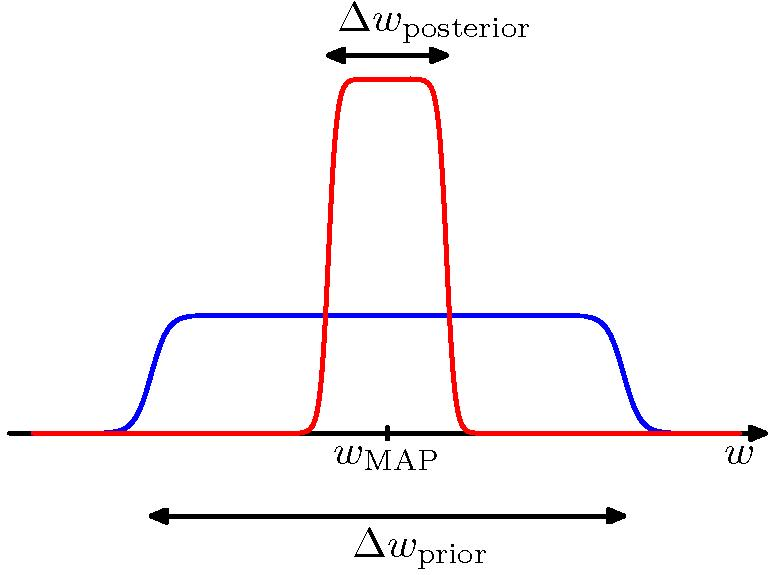
\includegraphics{prml/Figure3.12}
\end{SCfigure*}

and so taking logs
\begin{align}
\ln p(\mathcal{D}) \simeq \ln p(\mathcal{D}|w_{MAP}) +\ln(\dfrac{\Delta w_{posterior}}{\Delta w_{prior}})
\end{align}
If we have a set of $M$ parameters,assuming that all parameters have the same ratio of $\Delta w_{posterior}/\Delta w_{prior}$,we obtain
\begin{align}
\ln p(\mathcal{D}) \simeq \ln p(\mathcal{D}|w_{MAP}) +M\ln(\dfrac{\Delta w_{posterior}}{\Delta w_{prior}})
\end{align}
As we increase the complexity of the model,the first term representing the fit to the data,increases(?),whereas the second term will decrease due to the dependence on $M$.The optimal model is given by a trade-off between these two competing terms.
\begin{SCfigure*}
	\caption{Model complexity increases}
	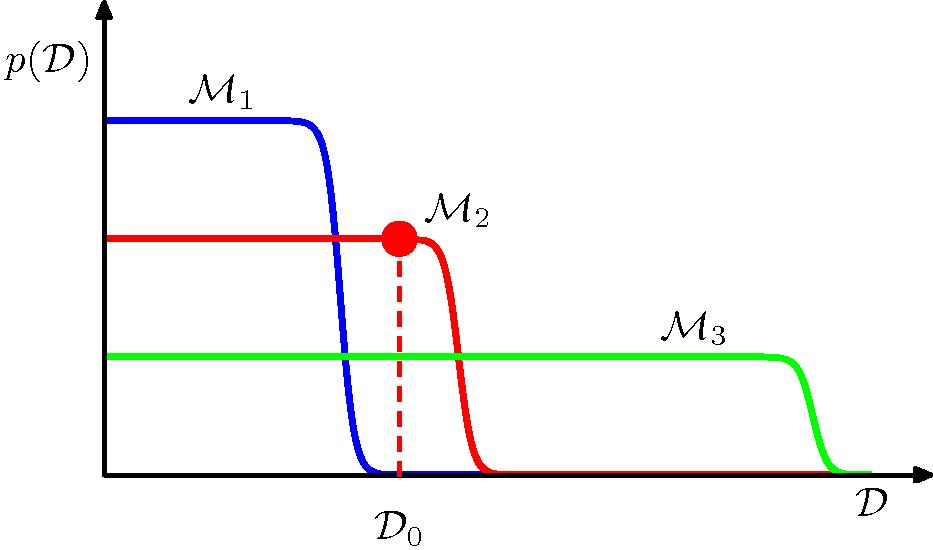
\includegraphics{prml/Figure3.13}
\end{SCfigure*}
Average the Bayes factor over the distribution of data sets
\begin{align}
\int p(\mathcal{D}|\mathcal{M}_1)\ln\dfrac{p(\mathcal{D}|\mathcal{M}_1)}{p(\mathcal{D}|\mathcal{M}_2)}
\end{align}
This quantity is $Kullback-Leibler$ divergence,and will be bigger than or equal to $0$ if $\mathcal{M}_1$ is the correct model.









































\input{"prml/Linear Models for Classification"}
\chapter{Logistic Regression}
\label{Logistic Regression}

\section{Representation}
Logistic regression can be binomial or multinomial. The \textbf{binomial logistic regression} model has the following form
\begin{equation}
p(y|\vec{x},\vec{w})=\mathrm{Ber}(y|\mathrm{sigm}(\vec{w}^T\vec{x}))
\end{equation}
where $\vec{w}$ and $\vec{x}$ are extended vectors, i.e., $\vec{w}=(b, w_1, w_2,\cdots, w_D)$, $\vec{x}=(1, x_1, x_2,\cdots, x_D)$.


\section{Optimization}
\label{sec:binomial-LR-Optimization}

\subsection{MLE}
\begin{align}
\ell(\vec{w}) &= \log\left\{\prod\limits_{i=1}^N{\left[\pi(\vec{x}_i)\right]^{y_i}\left[1-\pi(\vec{x}_i)\right]^{1-y_i}}\right\} \nonumber \\
              & \quad \text{, where } \pi(\vec{x}) \triangleq P(y=1|\vec{x},\vec{w}) \nonumber \\
           &= \sum\limits_{i=1}^N\left[y_i\log\pi(\vec{x}_i)+(1-y_i)\log(1-\pi(\vec{x}_i))\right] \label{eqn:cross-entropy-error} \nonumber \\
		   &= \sum\limits_{i=1}^N\left[y_i\log\dfrac{\pi(\vec{x}_i)}{1-\pi(\vec{x}_i)}+\log(1-\pi(\vec{x}_i))\right] \nonumber \\
		   &= \sum\limits_{i=1}^N\left[y_i(\vec{w}\cdot\vec{x}_i)-\log(1+\exp(\vec{w}\cdot\vec{x}_i))\right] \nonumber \\
J(\vec{w}) & \triangleq \mathrm{NLL}(\vec{w})= -\ell(\vec{w}) \nonumber \\
           & = -\sum\limits_{i=1}^N\left[y_i(\vec{w}\cdot\vec{x}_i)-\log(1+\exp(\vec{w}\cdot\vec{x}_i))\right] 
\end{align}

Equation \ref{eqn:cross-entropy-error} is also called the \textbf{cross-entropy} error function (see Equation \ref{eqn:cross-entropy}).

Unlike linear regression, we can no longer write down the MLE in closed form. Instead, we need to use an optimization algorithm to compute it, see Appendix \ref{chap:Optimization-methods}. For this, we need to derive the gradient and Hessian.

In the case of logistic regression, one can show that the gradient and Hessian of this are given by the following
\begin{align}
\vec{g}(\vec{w}) &= \dfrac{\mathrm{d} J}{\mathrm{d} \vec{w}} = \sum\limits_{i=1}^N \left[\pi(\vec{x}_i) - y_i \right]\vec{x}_i = \vec{X}(\vec{\pi}-\vec{y})\\
\vec{H}(\vec{w}) &= \dfrac{\mathrm{d} \vec{g}^T}{\mathrm{d} \vec{w}}= \dfrac{\mathrm{d}}{\mathrm{d} \vec{w}} (\vec{\pi}-\vec{y})^T\vec{X}^T \nonumber \\
        &= \dfrac{\mathrm{d}}{\mathrm{d} \vec{w}} \vec{\pi}^T\vec{X}^T \nonumber \\
		&= (\pi(\vec{x}_i)(1-\pi(\vec{x}_i))\vec{x}_i, \cdots,)\vec{X}^T \nonumber \\
		&= \vec{X}\vec{S}\vec{X}^T, \quad \vec{S} \triangleq \mathrm{diag}(\pi(\vec{x}_i)(1-\pi(\vec{x}_i))\vec{x}_i)
\end{align}


\subsubsection{Iteratively reweighted least squares (IRLS)}
\label{sec:IRLS}
TODO


\subsection{MAP}
Just as we prefer ridge regression to linear regression, so we should prefer MAP estimation for logistic regression to computing the MLE. 
$\ell_2$ regularization

we can use $\ell_2$ regularization, just as we did with ridge regression. We note that the new objective, gradient and Hessian have the following forms:
\begin{align}
J'(\vec{w}) & \triangleq \mathrm{NLL}(\vec{w})+\lambda \vec{w}^T\vec{w} \\
\vec{g}'(\vec{w}) &= \vec{g}(\vec{w})+\lambda\vec{w} \\
\vec{H}'(\vec{w}) &= \vec{H}(\vec{w})+\lambda\vec{I}
\end{align}

It is a simple matter to pass these modified equations into any gradient-based optimizer.


\section{Multinomial logistic regression}


\subsection{Representation}
\textbf{Multinomial logistic regression} model is also called a \textbf{maximum entropy classifier}, which has the following form
\begin{align}
p(y=c|\vec{x},\vec{W}) & =\dfrac{\exp(\vec{w}_c^T\vec{x})}{\sum_{c=1}^C \exp(\vec{w}_c^T\vec{x})}
\end{align}


\subsection{MLE}
Let $\vec{y}_i=(\mathbb{I}(y_i=1),\mathbb{I}(y_i=1),\cdots, \mathbb{I}(y_i=C))$, $\vec{\mu}_i=(p(y=1|\vec{x}_i,\vec{W}),p(y=2|\vec{x}_i,\vec{W}),\cdots, p(y=C|\vec{x}_i,\vec{W}))$, then the log-likelihood function can be written as
\begin{align}
\ell(\vec{W}) & =\log\prod\limits_{i=1}^N\prod\limits_{c=1}^C \mu_{ic}^{y_{ic}}=\sum\limits_{i=1}^N\sum\limits_{c=1}^C y_{ic}\log \mu_{ic} \\
     & = \sum\limits_{i=1}^N\left[\left(\sum\limits_{c=1}^C y_{ic}\vec{w}_c^T\vec{x}_i\right)-\log\left(\sum\limits_{c=1}^C \exp(\vec{w}_c^T\vec{x}_i)\right)\right]
\end{align}

Define the objective function as NLL
\begin{equation}
J(\vec{W})=\mathrm{NLL}(\vec{W})=-\ell(\vec{W})
\end{equation}

Define $\vec{A} \otimes \vec{B}$ be the \textbf{kronecker product} of matrices $\vec{A}$ and $\vec{B}$.If $\vec{A}$ is an $m \times n$ matrix and $\vec{B}$ is a $p \times q$ matrix, then $\vec{A} \otimes \vec{B}$ is the $mp \times nq$ block matrix
\begin{equation}
\vec{A} \otimes \vec{B} \triangle \left(\begin{array}{ccc}
a_{11}\vec{B} & \cdots & a_{1n}\vec{B} \\
\vdots & \vdots & \vdots \\
a_{m1}\vec{B} & \cdots & a_{mn}\vec{B}
\end{array}\right)
\end{equation}

The gradient and Hessian are given by
\begin{align}
\vec{g}(\vec{W}) & =\sum\limits_{i=1}^N (\vec{\mu}-\vec{y}_i) \otimes \vec{x}_i \\
\vec{H}(\vec{W}) & =\sum\limits_{i=1}^N (\mathrm{diag}(\vec{\mu}_i)-\vec{\mu}_i\vec{\mu}_i^T) \otimes (\vec{x}_i\vec{x}_i^T)
\end{align}
where $\vec{y}_i=(\mathbb{I}(y_i=1),\mathbb{I}(y_i=1),\cdots, \mathbb{I}(y_i=C-1))$ and $\vec{\mu}_i=(p(y=1|\vec{x}_i,\vec{W}),p(y=2|\vec{x}_i,\vec{W}),\cdots, p(y=C-1|\vec{x}_i,\vec{W}))$ are column vectors of length $C-1$.

Pass them to any gradient-based optimizer.


\subsection{MAP}
The new objective
\begin{align}
J'(\vec{W}) & =\mathrm{NLL}(\vec{w})-\log{p(\vec{W})} \\
            & \quad \text{, where } p(\vec{W}) \triangleq \prod\limits_{c=1}^C \mathcal{N}(\vec{w}_c|\vec{0},\vec{V}_0) \nonumber \\
   & = J(\vec{W})+\dfrac{1}{2}\sum\limits_{c=1}^C \vec{w}_c\vec{V}_0^{-1}\vec{w}_c \\
\end{align}

Its gradient and Hessian are given by
\begin{align}
\vec{g}'(\vec{w}) & =\vec{g}(\vec{W})+\vec{V}_0^{-1}\left(\sum\limits_{c=1}^C \vec{w}_c\right) \\
\vec{H}'(\vec{w}) & =\vec{H}(\vec{w})+\vec{I_C} \otimes \vec{V}_0^{-1}
\end{align}

This can be passed to any gradient-based optimizer to find the MAP estimate. Note, however, that the Hessian has size $((CD)×(CD))$, which is $C$ times more row and columns than in the binary case, so limited memory BFGS is more appropriate than Newton’s method.


\section{Bayesian logistic regression}
It is natural to want to compute the full posterior over the parameters, $p(\vec{w}|\mathcal{D})$, for logistic regression models. This can be useful for any situation where we want to associate confidence intervals with our predictions (e.g., this is necessary when solving contextual bandit problems, discussed in Section TODO).

Unfortunately, unlike the linear regression case, this cannot be done exactly, since there is no convenient conjugate prior for logistic regression. We discuss one simple approximation below; some other approaches include MCMC (Section TODO), variational inference (Section TODO), expectation propagation (Kuss and Rasmussen 2005), etc. For notational simplicity, we stick to binary logistic regression.


\subsection{Laplace approximation}


\subsection{Derivation of the BIC}


\subsection{Gaussian approximation for logistic regression}
\label{sec:Gaussian-approximation-for-logistic-regression}


\subsection{Approximating the posterior predictive}


\subsection{Residual analysis (outlier detection) *}


\section{Online learning and stochastic optimization}
Traditionally machine learning is performed \textbf{offline}, however, if we have \textbf{streaming data}, we need to perform \textbf{online learning}, so we can update our estimates as each new data point arrives rather than waiting until “the end” (which may never occur). And even if we have a batch of data, we might want to treat it like a stream if it is too large to hold in main memory. Below we discuss learning methods for this kind of scenario.

TODO


\subsection{The perceptron algorithm}

\subsubsection{Representation}
\begin{equation}
\mathcal{H}:y=f(\vec{x})=\text{sign}(\vec{w}^T\vec{x}+b)
\end{equation}
where $\text{sign}(x)=\begin{cases}+1, & x \geq 0\\-1, & x<0\\\end{cases}$, see Fig. \ref{fig:perceptron}\footnote{\url{https://en.wikipedia.org/wiki/Perceptron}}.

\begin{figure}[hbtp]
\centering
    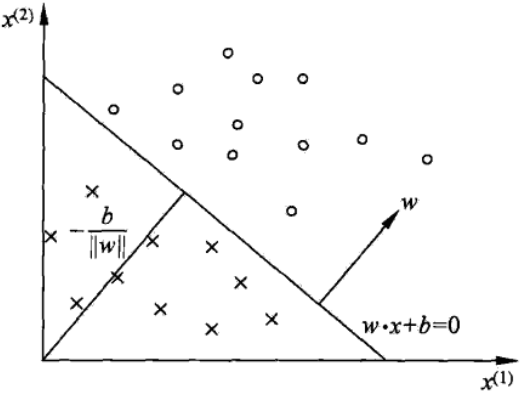
\includegraphics[scale=.50]{perceptron.png}
\caption{Perceptron}
\label{fig:perceptron} 
\end{figure}


\subsubsection{Evaluation}
\begin{eqnarray}
L(\vec{w},b)&=&-y_i(\vec{w}^T\vec{x}_i+b)\\
R_{emp}(f)&=&-\sum\limits_i y_i(\vec{w}^T\vec{x}_i+b)\\
\end{eqnarray}


\subsubsection{Optimization}
\textbf{Primal form}
\begin{algorithm}[htbp]
\caption{Perceptron learning algorithm, primal form, using SGD}
  
    $\vec{w} \leftarrow 0;\; b \leftarrow 0;\; k \leftarrow 0$\;
    \While{no mistakes made within the for loop}{
        \For{$i\leftarrow 1$ \KwTo $N$}{
			\If{$y_i(\vec{w} \cdot \vec{x}_i+b) \leq 0$}{
				$\vec{w} \leftarrow \vec{w}+\eta y_i \vec{x}_i$\;
				$b \leftarrow b+\eta y_i$\;
				$k \leftarrow k+1$\;
			}
		}
    }
\end{algorithm}

\textbf{Convergency}
\begin{theorem}
(\textbf{Novikoff}) If traning data set $\mathcal{D}$ is linearly separable, then
\begin{enumerate}
\item There exists a hyperplane denoted as $\widehat{\vec{w}}_{opt} \cdot \vec{x}+b_{opt}=0$ which can correctly seperate all samples, and 
\begin{equation}
\exists\gamma>0,\; \forall i, \; y_i(\vec{w}_{opt} \cdot \vec{x}_i+b_{opt}) \geq \gamma
\end{equation}
\item \begin{equation}k \leq \left(\dfrac{R}{\gamma}\right)^2,\text{ where } R=\max\limits_{1 \leq i \leq N} \abs{\abs{\widehat{\vec{x}}_i}}
\end{equation}
\end{enumerate}
\end{theorem}

\begin{proof}
(1) let $\gamma=\min\limits_{i} y_i(\vec{w}_{opt} \cdot \vec{x}_i+b_{opt})$, then we get $y_i(\vec{w}_{opt} \cdot \vec{x}_i+b_{opt}) \geq \gamma$.

(2) The algorithm start from $\widehat{\vec{x}}_0=0$, if a instance is misclassified, then update the weight. Let $\widehat{\vec{w}}_{k-1}$ denotes the extended weight before the k-th misclassified instance, then we can get
\begin{eqnarray}
y_i(\widehat{\vec{w}}_{k-1} \cdot \widehat{\vec{x}_i})&=&y_i(\vec{w}_{k-1} \cdot \vec{x}_i+b_{k-1}) \leq 0\\
\widehat{\vec{w}}_k&=&\widehat{\vec{w}}_{k-1}+\eta y_i \widehat{\vec{x}_i}
\end{eqnarray}

We could infer the following two equations, the proof procedure are omitted.
\begin{enumerate}
\item $\widehat{\vec{w}}_k \cdot \widehat{\vec{w}}_{opt} \geq k\eta\gamma$
\item $\abs{\abs{\widehat{\vec{w}}_k}}^2 \leq k\eta^2R^2$
\end{enumerate}

From above two equations we get
\begin{eqnarray}
\nonumber k\eta\gamma & \leq & \widehat{\vec{w}}_k \cdot \widehat{\vec{w}}_{opt} \leq \abs{\abs{\widehat{\vec{w}}_k}}\abs{\abs{\widehat{\vec{w}}_{opt}}} \leq \sqrt k \eta R \\
\nonumber k^2\gamma^2 & \leq & kR^2 \\
\nonumber \text{i.e. } k & \leq & \left(\dfrac{R}{\gamma}\right)^2
\end{eqnarray}
\end{proof}


\textbf{Dual form}
\begin{eqnarray}
\vec{w}&=&\sum\limits_{i=1}^{N} \alpha_iy_i\vec{x}_i \\
b&=&\sum\limits_{i=1}^{N} \alpha_iy_i \\
f(\vec{x})&=&\text{sign}\left(\sum\limits_{j=1}^{N} \alpha_jy_j\vec{x}_j \cdot \vec{x}+b\right)
\end{eqnarray}

\begin{algorithm}[htbp]
    %\SetAlgoLined
    \SetAlgoNoLine
  
    $\vec{\alpha} \leftarrow 0;\; b \leftarrow 0;\; k \leftarrow 0$\;
    \While{no mistakes made within the for loop}{
        \For{$i\leftarrow 1$ \KwTo $N$}{
			\If{$y_i\left(\sum\limits_{j=1}^{N} \alpha_jy_j\vec{x}_j \cdot \vec{x}_i+b\right) \leq 0$}{
				$\vec{\alpha} \leftarrow \vec{\alpha}+\eta$\;
				$b \leftarrow b+\eta y_i$\;
				$k \leftarrow k+1$\;
			}
		}
    }
\caption{Perceptron learning algorithm, dual form}
\end{algorithm}


\section{Generative vs discriminative classifiers}


\subsection{Pros and cons of each approach}
\begin{itemize}
\item{\textbf{Easy to fit?} As we have seen, it is usually very easy to fit generative classifiers. For example, in Sections \ref{sec:NBC-Optimization} and \ref{sec:MLE-for-discriminant-analysis}, we show that we can fit a naive Bayes model and an LDA model by simple counting and averaging. By contrast, logistic regression requires solving a convex optimization problem (see Section \ref{sec:binomial-LR-Optimization} for the details), which is much slower.}

\item{\textbf{Fit classes separately?} In a generative classifier, we estimate the parameters of each class conditional density independently, so we do not have to retrain the model when we add more classes. In contrast, in discriminative models, all the parameters interact, so the whole model must be retrained if we add a new class. (This is also the case if we train a generative model to maximize a discriminative objective Salojarvi et al. (2005).)}

\item{\textbf{Handle missing features easily?} Sometimes some of the inputs (components ofx) are not observed. In a generative classifier, there is a simple method for dealing with this, as we discuss in Section \ref{sec:Dealing-with-missing-data}. However, in a discriminative classifier, there is no principled solution to this problem, since the model assumes that $\vec{x}$is always available to be conditioned on (although see (Marlin 2008) for some heuristic approaches).}

\item{\textbf{Can handle unlabeled training data?} There is much interest in \textbf{semi-supervised learning}, which uses unlabeled data to help solve a supervised task. This is fairly easy to do using generative models (see e.g., (Lasserre et al. 2006; Liang et al. 2007)), but is much harder to do with discriminative models.}

\item{\textbf{Symmetric in inputs and outputs?} We can run a generative model “backwards”, and infer probable inputs given the output by computing $p(\vec{x}|y)$. This is not possible with a discriminative model. The reason is that a generative model defines a joint distribution on $\vec{x}$ and $y$, and hence treats both inputs and outputs symmetrically.}

\item{\textbf{Can handle feature preprocessing?} A big advantage of discriminative methods is that they allow us to preprocess the input in arbitrary ways, e.g., we can replace $\vec{x}$ with $\phi(\vec{x})$, which could be some basis function expansion, etc. It is often hard to define a generative model on such pre-processed data, since the new features are correlated in complex ways.}

\item{\textbf{Well-calibrated probabilities?} Some generative models, such as naive Bayes, make strong independence assumptions which are often not valid. This can result in very extreme posterior class probabilities (very near 0 or 1). Discriminative models, such as logistic regression, are usually better calibrated in terms of their probability estimates.}
\end{itemize}

See Table \ref{tab:List-of-various-models-for-classification} for a summary of the classification and regression techniques we cover in this book.

\begin{table*}
\centering
\begin{tabular}{lllll}
\hline\noalign{\smallskip}
\textbf{Model} & \textbf{Classif/regr} & \textbf{Gen/Discr} & \textbf{Param/Non} & \textbf{Section} \\
\noalign{\smallskip}\svhline\noalign{\smallskip}
Discriminant analysis & Classif & Gen & Param & Sec. \ref{sec:Linear-discriminant-analysis}, \ref{sec:MLE-for-discriminant-analysis} \\
Naive Bayes classifier & Classif & Gen & Param & Sec. \ref{sec:NBC}, \ref{sec:Bayesian-naive-Bayes} \\
Tree-augmented Naive Bayes classifier & Classif & Gen & Param & Sec. 10.2.1 \\
Linear regression & Regr & Discrim & Param & Sec. 1.4.5, 7.3, 7.6 \\
Logistic regression & Classif & Discrim & Param & Sec. 1.4.6, \ref{sec:IRLS}, \ref{sec:Gaussian-approximation-for-logistic-regression}, 21.8.1.1 \\
Sparse linear/ logistic regression & Both & Discrim & Param & Ch. 13 \\
Mixture of experts & Both & Discrim & Param & Sec. 11.2.4 \\
Multilayer perceptron (MLP)/ Neural network & Both & Discrim & Param & Ch. 16 \\
Conditional random field (CRF) & Classif & Discrim & Param & Sec. 19.6 \\
\noalign{\smallskip}\hline \\
$K$ nearest neighbor classifier & Classif & Gen & Non & Sec. TODO, TODO \\
(Infinite) Mixture Discriminant analysis & Classif & Gen & Non & Sec. 14.7.3 \\
Classification and regression trees (CART) & Both & Discrim & Non & Sec. 16.2 \\
Boosted model & Both & Discrim & Non & Sec. 16.4 \\
Sparse kernelized lin/logreg (SKLR) & Both & Discrim & Non & Sec. 14.3.2 \\
Relevance vector machine (RVM) & Both & Discrim & Non & Sec. 14.3.2 \\
Support vector machine (SVM) & Both & Discrim & Non & Sec. 14.5 \\
Gaussian processes (GP) & Both & Discrim & Non & Ch. 15 \\
Smoothing splines & Regr & Discrim & Non & Section 15.4.6 \\
\noalign{\smallskip}\hline
\end{tabular}
\caption{List of various models for classification and regression which we discuss in this book. Columns are as follows: Model name; is the model suitable for classification, regression, or both; is the model generative or discriminative; is the model parametric or non-parametric; list of sections in book which discuss the model. See also \url{http://pmtk3.googlecode.com/svn/trunk/docs/tutorial/html/tutSupervised.html} for the PMTK equivalents of these models. Any generative probabilistic model (e.g., HMMs, Boltzmann machines, Bayesian networks, etc.) can be turned into a classifier by using it as a class conditional density}
\label{tab:List-of-various-models-for-classification}
\end{table*}


\subsection{Dealing with missing data}
\label{sec:Dealing-with-missing-data}
Sometimes some of the inputs (components of $\vec{x}$) are not observed; this could be due to a sensor failure, or a failure to complete an entry in a survey, etc. This is called the \textbf{missing data problem} (Little. and Rubin 1987). The ability to handle missing data in a principled way is one of the biggest advantages of generative models.

To formalize our assumptions, we can associate a binary response variable $r_i \in \{0,1\}$ that specifies whether each value $\vec{x}_i$ is observed or not. The joint model has the form $p(\vec{x}_i,r_i|\vec{\theta},\vec{\phi})=p(r_i|\vec{x}_i,\vec{\phi})p(\vec{x}_i|\vec{\theta})$, where $\vec{\phi}$ are the parameters controlling whether the item is observed or not. 
\begin{itemize}
\item{If we assume $p(r_i|\vec{x}_i,\vec{\phi})=p(r_i|\vec{\phi})$, we say the data is \textbf{missing completely at random} or \textbf{MCAR}.}
\item{If we assume $p(r_i|\vec{x}_i,\vec{\phi})=p(r_i|\vec{x}_i^o,\vec{\phi})$, where $\vec{x}_i^o$ is the observed part of $\vec{x}_i$, we say the data is \textbf{missing at random} or \textbf{MAR}.}
\item{If neither of these assumptions hold, we say the data is \textbf{not missing at random} or \textbf{NMAR}. In this case, we have to model the missing data mechanism, since the pattern of missingness is informative about the values of the missing data and the corresponding parameters. This is the case in most collaborative filtering problems, for example.}
\end{itemize}

See e.g., (Marlin 2008) for further discussion. We will henceforth assume the data is MAR.

When dealing with missing data, it is helpful to distinguish the cases when there is missingness only at test time (so the training data is \textbf{complete data}), from the harder case when there is missingness also at training time. We will discuss these two cases below. Note that the class label is always missing at test time, by definition; if the class label is also sometimes missing at training time, the problem is called semi-supervised learning.


\subsubsection{Missing data at test time}
In a generative classifier, we can handle features that are MAR by marginalizing them out. For example, if we are missing the value ofx1, we can compute
\begin{align}
p(y=c|\vec{x}_{2:D},\vec{\theta}) & \propto p(y=c|\vec{\theta})p(\vec{x}_{2:D}|y=c,\vec{\theta}) \\
      & = \propto p(y=c|\vec{\theta})\sum\limits_{x_1}p(x_1, \vec{x}_{2:D}|y=c,\vec{\theta})
\end{align}

Similarly, in discriminant analysis, no matter what regularization method was used to estimate the parameters, we can always analytically marginalize out the missing variables (see Section \ref{sec:Inference-in-jointly-Gaussian-distributions}):
\begin{equation}
p(\vec{x}_{2:D}|y=c,\vec{\theta})=\mathcal{N}(\vec{x}_{2:D}|\vec{\mu}_{c,2:D},\vec{\Sigma}_{c,2:D})
\end{equation}


\subsubsection{Missing data at training time}
Missing data at training time is harder to deal with. In particular, computing the MLE or MAP estimate is no longer a simple optimization problem, for reasons discussed in Section TODO. However, soon we will study are a variety of more sophisticated algorithms (such as EM algorithm, in Section 11.4) for finding approximate ML or MAP estimates in such cases.


\subsection{Fisher’s linear discriminant analysis (FLDA) *}
TODO
%\input{"ml/Directed graphical models (Bayes nets)"}
\input{"prml/Mixture models and EM"}
%\chapter{Latent linear models}


\section{Factor analysis}
One problem with mixture models is that they only use a single latent variable to generate the observations. In particular, each observation can only come from one of $K$ prototypes. One can think of a mixture model as using $K$ hidden binary variables, representing a one-hot encoding of the cluster identity. But because these variables are mutually exclusive, the model is still limited in its representational power.

An alternative is to use a vector of real-valued latent variables,$\vec{z}_i \in \mathbb{R}^L$. The simplest prior to use is a Gaussian (we will consider other choices later):
\begin{equation}\label{eqn:FA-prior}
p(\vec{z}_i)=\mathcal{N}(\vec{z}_i|\vec{\mu}_0,\vec{\Sigma}_0)
\end{equation}
If the observations are also continuous, so $\vec{x}_i \in \mathbb{R}^D$, we may use a Gaussian for the likelihood. Just as in linear regression, we will assume the mean is a linear function of the (hidden) inputs, thus yielding
\begin{equation}\label{eqn:FA-class-conditional-density}
p(\vec{x}_i|\vec{z}_i,\vec{\theta})=\mathcal{N}(\vec{x}_i|\vec{W}\vec{z}_i+\vec{\mu},\vec{\Psi})
\end{equation}
where \vec{W} is a $D \times L$ matrix, known as the \textbf{factor loading matrix}, and $\vec{\Psi}$ is a $D \times D$ covariance matrix. We take $\vec{\Psi}$ to be diagonal, since the whole point of the model is to “force” $\vec{z}_i$ to explain the correlation, rather than “baking it in” to the observation’s covariance. This overall model is called \textbf{factor analysis} or \textbf{FA}. The special case in which $\vec{\Psi}=\sigma^2\vec{I}$ is called \textbf{probabilistic principal components analysis} or \textbf{PPCA}. The reason for this name will become apparent later.


\subsection{FA is a low rank parameterization of an MVN}
FA can be thought of as a way of specifying a joint density model on $\vec{x}$ using a small number of parameters. To see this, note that from Equation \ref{eqn:Linear-Gaussian-system-normalizer}, the induced marginal distribution $p(\vec{x}_i|\vec{\theta})$ is a Gaussian:
\begin{align}
p(\vec{x}_i|\vec{\theta}) & = \int \mathcal{N}(\vec{x}_i|\vec{W}\vec{z}_i+\vec{\mu},\vec{\Psi})\mathcal{N}(\vec{z}_i|\vec{\mu}_0,\vec{\Sigma}_0)\mathrm{d}\vec{z}_i \nonumber \\
 & = \mathcal{N}(\vec{x}_i|\vec{W}\vec{\mu}_0+\vec{\mu},\vec{\Psi}+\vec{W}\vec{\Sigma}_0\vec{W})
\end{align}
From this, we see that we can set $\vec{\mu}_0=0$ without loss of generality, since we can always absorb $\vec{W}\vec{\mu}_0$ into $\vec{\mu}$. Similarly, we can set $\vec{\Sigma}_0=\vec{I}$ without loss of generality, because we can always “emulate” a correlated prior by using defining a new weight matrix, $\tilde{\vec{W}}=\vec{W}\vec{\Sigma}_0^{-\frac{1}{2}}$. So we can rewrite Equation \ref{eqn:FA-prior} and \ref{eqn:FA-class-conditional-density} as:
\begin{align}
p(\vec{z}_i)&=\mathcal{N}(\vec{z}_i|\vec{0},\vec{I}) \\
p(\vec{x}_i|\vec{z}_i,\vec{\theta})&=\mathcal{N}(\vec{x}_i|\vec{W}\vec{z}_i+\vec{\mu},\vec{\Psi})
\end{align}

We thus see that FA approximates the covariance matrix of the visible vector using a low-rank decomposition:
\begin{equation}\label{eqn:FA-prior}
\vec{C} \triangleq \mathrm{cov}[\vec{x}]=\vec{W}\vec{W}^T+\vec{\Psi}
\end{equation}
This only uses $O(LD)$ parameters, which allows a flexible compromise between a full covariance Gaussian, with $O(D^2)$ parameters, and a diagonal covariance, with $O(D)$ parameters. Note that if we did not restrict $\vec{\Psi}$ to be diagonal, we could trivially set $\vec{\Psi}$ to a full covariance matrix; then we could set $\vec{W}=0$, in which case the latent factors would not be required.


\subsection{Inference of the latent factors}
\begin{align}
p(\vec{z}_i|\vec{x}_i,\vec{\theta}) & = \mathcal{N}(\vec{z}_i|\vec{\mu}_i,\vec{\Sigma}_i) \\
\vec{\Sigma}_i & \triangleq (\vec{\Sigma}_0^{-1}+\vec{W}^T\vec{\Psi}^{-1}\vec{W})^{-1} \\
               & =(\vec{I}+\vec{W}^T\vec{\Psi}^{-1}\vec{W})^{-1} \\
\vec{\mu}_i & \triangleq \vec{\Sigma}_i[\vec{W}^T\vec{\Psi}^{-1}(\vec{x}_i-\vec{\mu})+\vec{\Sigma}_0^{-1}\vec{\mu}_0] \\
            & =\vec{\Sigma}_i\vec{W}^T\vec{\Psi}^{-1}(\vec{x}_i-\vec{\mu})
\end{align}
Note that in the FA model, $\vec{\Sigma}_i$ is actually independent of $i$, so we can denote it by $\vec{\Sigma}$. Computing this matrix takes $O(L^3+L^2D)$ time, and computing each $\vec{\mu}_i=\mathbb{E}[\vec{z}_i|\vec{x}_i,\vec{\theta}]$ takes $O(L^2+LD)$ time. The $\vec{\mu}_i$ are sometimes called the \textbf{latent scores}, or \textbf{latent factors}.


\subsection{Unidentifiability}
Just like with mixture models, FA is also unidentifiable. To see this, suppose $\vec{R}$ is an arbitrary orthogonal rotation matrix, satisfying $\vec{R}\vec{R}^T=\vec{I}$. Let us define $\tilde{\vec{W}}=\vec{W}\vec{R}$, then the likelihood function of this modified matrix is the same as for the unmodified matrix, since $\vec{W}\vec{R}\vec{R}^T\vec{W}^T+\vec{\Psi}=\vec{W}\vec{W}^T+\vec{\Psi}$. Geometrically, multiplying $\vec{W}$ by an orthogonal matrix is like rotating $\vec{z}$ before generating $\vec{x}$.

To ensure a unique solution, we need to remove $L(L-1)/2$ degrees of freedom, since that is the number of orthonormal matrices of size $L \times L$.\footnote{To see this, note that there are $L-1$ free parameters in $\vec{R}$ in the first column (since the column vector must be normalized to unit length), there are $L-2$ free parameters in the second column (which must be orthogonal to the first), and so on.} In total, the FA model has $D+LD-L(L-1)/2$ free parameters (excluding the mean), where the first term arises from $\vec{\Psi}$. Obviously we require this to be less than or equal to $D(D+1)/2$, which is the number of parameters in an unconstrained (but symmetric) covariance matrix. This gives us an upper bound on $L$, as follows:
\begin{equation}
L_{\mathrm{max}}=\lfloor D+0.5(1-\sqrt{1+8D}) \rfloor
\end{equation}

For example, $D=6$ implies $L \leq 3$. But we usually never choose this upper bound, since it would result in overfitting (see discussion in Section \ref{sec:FA-Choosing-L} on how to choose $L$).


Unfortunately, even if we set $L < L_{\mathrm{max}}$, we still cannot uniquely identify the parameters, since the rotational ambiguity still exists. Non-identifiability does not affect the predictive performance of the model. However, it does affect the loading matrix, and hence the interpretation of the latent factors. Since factor analysis is often used to uncover structure in the data, this problem needs to be addressed. Here are some commonly used solutions:
\begin{itemize}
\item{\textbf{Forcing $\vec{W}$ to be orthonormal} Perhaps the cleanest solution to the identifiability problem is to force $\vec{W}$ to be orthonormal, and to order the columns by decreasing variance of the corresponding latent factors. This is the approach adopted by PCA, which we will discuss in Section \ref{sec:PCA}. The result is not necessarily more interpretable, but at least it is unique.}
\item{\textbf{Forcing $\vec{W}$ to be lower triangular} One way to achieve identifiability, which is popular in the Bayesian community (e.g., (Lopes and West 2004)), is to ensure that the first visible feature is only generated by the first latent factor, the second visible feature is only generated by the first two latent factors, and so on. For example, if $L=3$ and $D=4$, the correspond factor loading matrix is given by
\begin{equation*}
\vec{W}=\left(\begin{array}{ccc}
w_{11} & 0 & 0 \\
w_{21} & w_{22} & 0 \\
w_{31} & w_{32} & w_{33} \\
w_{41} & w_{32} & w_{43}
\end{array}\right)
\end{equation*}
We also require that $w_{jj} >0$ for $j =1:L$. The total number of parameters in this constrained matrix is $D+DL-L(L-1)/2$, which is equal to the number of uniquely identifiable parameters. The disadvantage of this method is that the first $L$ visible variables, known as the \textbf{founder variables}, affect the interpretation of the latent factors, and so must be chosen carefully.}
\item{\textbf{Sparsity promoting priors on the weights} Instead of pre-specifying which entries in $\vec{W}$ are zero, we can encourage the entries to be zero, using $\ell_1$ regularization (Zou et al. 2006), ARD (Bishop 1999; Archambeau and Bach 2008), or spike-and-slab priors (Rattray et al. 2009). This is called sparse factor analysis. This does not necessarily ensure a unique MAP estimate, but it does encourage interpretable solutions. See Section 13.8 TODO.}
\item{\textbf{Choosing an informative rotation matrix} There are a variety of heuristic methods that try to find rotation matrices $\vec{R}$ which can be used to modify $\vec{W}$(and hence the latent factors) so as to try to increase the interpretability, typically by encouraging them to be (approximately) sparse. One popular method is known as \textbf{varimax}(Kaiser 1958).}
\item{\textbf{Use of non-Gaussian priors for the latent factors} In Section \ref{sec:ICA}, we will dicuss how replacing $p(\vec{z}_i)$ with a non-Gaussian distribution can enable us to sometimes uniquely identify $\vec{W}$ as well as the latent factors. This technique is known as ICA.}
\end{itemize}


\subsection{Mixtures of factor analysers}
The FA model assumes that the data lives on a low dimensional linear manifold. In reality, most
data is better modeled by some form of low dimensional \emph{curved} manifold. We can approximate a curved manifold by a piecewise linear manifold. This suggests the following model: let the $k$'th linear subspace of dimensionality $L_k$ be represented by $\vec{W}_k$, for $k=1:K$. Suppose we have a latent indicator $qi \in \{1,\cdots,K\}$ specifying which subspace we should use to generate the data. We then sample $\vec{z}_i$ from a Gaussian prior and pass it through the $\vec{W}_k$ matrix (where $k=q_i$), and add noise. More precisely, the model is as follows:
\begin{align}
p(q_i|\vec{\theta}) & =\mathrm{Cat}(q_i\vec{\pi}) \\
p(\vec{z}_i|\vec{\theta}) & =\mathcal{N}(\vec{z}_i|\vec{0},\vec{I}) \\
p(\vec{x}_i|q_i=k,\vec{z}_i,\vec{\theta}) & =\mathcal{N}(\vec{x}_i|\vec{W}\vec{z}_i+\vec{\mu}_k,\vec{\Psi})
\end{align}
This is called a \textbf{mixture of factor analysers}(MFA) (Hinton et al. 1997).

Another way to think about this model is as a low-rank version of a mixture of Gaussians. In particular, this model needs $O(KLD)$ parameters instead of the $O(KD^2)$ parameters needed for a mixture of full covariance Gaussians. This can reduce overfitting. In fact, MFA is a good generic density model for high-dimensional real-valued data.


\subsection{EM for factor analysis models}
Below we state the results without proof. The derivation can be found in (Ghahramani and Hinton 1996a). To obtain the results for a single factor analyser, just set $r_{ic} =1$ and $c=1$ in the equations below. In Section \ref{sec:EM-for-PCA} we will see a further simplification of these equations that arises when fitting a PPCA model, where the results will turn out to have a particularly simple and elegant interpretation.

In the E-step, we compute the posterior responsibility of cluster $k$ for data point $i$ using
\begin{equation}
r_{ik} \triangleq p(q_i=k|\vec{x}_i,\vec{\theta}) \propto \pi_k\mathcal{N}(\vec{x}_i|\vec{\mu}_k,\vec{W}_k\vec{W}_k^T\vec{\Psi}_k)
\end{equation}

The conditional posterior for $\vec{z}_i$ is given by
\begin{align}
p(\vec{z}_i|\vec{x}_i,q_i=k,\vec{\theta}) & = \mathcal{N}(\vec{z}_i|\vec{\mu}_{ik},\vec{\Sigma}_{ik}) \\
\vec{\Sigma}_{ik} & \triangleq (\vec{I}+\vec{W}_k^T\vec{\Psi}_k^{-1}\vec{W})_k^{-1} \\
\vec{\mu}_{ik} & \triangleq \vec{\Sigma}_{ik}\vec{W}_k^T\vec{\Psi}_k^{-1}(\vec{x}_i-\vec{\mu}_k)
\end{align}

In the M step, it is easiest to estimate $\vec{\mu}_k$ and $\vec{W}_k$ at the same time, by defining $\tilde{\vec{W}}_k=(\vec{W}_k,\vec{\mu}_k)$, $\tilde{\vec{z}}=(\vec{z},1)$, also, define
\begin{align}
\tilde{\vec{W}}_k & =(\vec{W}_k,\vec{\mu}_k) \\
\tilde{\vec{z}} & =(\vec{z},1) \\
\vec{b}_{ik} & \triangleq \mathbb{E}[\tilde{\vec{z}}|\vec{x}_i,q_i=k]=\mathbb{E}[(\vec{\mu}_{ik};1)] \\
\vec{C}_{ik} & \triangleq \mathbb{E}[\tilde{\vec{z}}\tilde{\vec{z}}^T|\vec{x}_i,q_i=k] \\
    & =\left(\begin{array}{cc}
\mathbb{E}[\vec{z}\vec{z}^T|\vec{x}_i,q_i=k] & \mathbb{E}[\vec{z}|\vec{x}_i,q_i=k] \\
\mathbb{E}[\vec{z}|\vec{x}_i,q_i=k]^T & 1
\end{array}\right)
\end{align}
Then the M step is as follows:
\begin{align}
\hat{\pi}_k & = \frac{1}{N}\sum\limits_{i=1}^N r_{ik} \\
\hat{\tilde{\vec{W}}}_k & = \left(\sum\limits_{i=1}^N r_{ik}\vec{x}_i\vec{b}_{ik}^T\right)\left(\sum\limits_{i=1}^N r_{ik}\vec{x}_i\vec{C}_{ik}^T\right)^{-1} \label{eqn:FA-EM-W} \\
\hat{\vec{\Psi}} & = \frac{1}{N}\mathrm{diag}\left[\sum\limits_{i=1}^N r_{ik}(\vec{x}_i-\hat{\tilde{\vec{W}}}_{ik}\vec{b}_{ik})\vec{x}_i^T\right]
\end{align}

Note that these updates are for “vanilla” EM. A much faster version of this algorithm, based on ECM, is described in (Zhao and Yu 2008).


\subsection{Fitting FA models with missing data}
\label{sec:Fitting-FA-models-with-missing-data}
In many applications, such as collaborative filtering, we have missing data. One virtue of the EM approach to fitting an FA/PPCA model is that it is easy to extend to this case. However, overfitting can be a problem if there is a lot of missing data. Consequently it is important to perform MAP estimation or to use Bayesian inference. See e.g., (Ilin and Raiko 2010) for details.


\section{Principal components analysis (PCA)}
\label{sec:PCA}
Consider the FA model where we constrain $\vec{\Psi}=\sigma^2\vec{I}$, and $\vec{W}$ to be orthonormal. It can be shown (Tipping and Bishop 1999) that, as $\sigma^2 \rightarrow 0$, this model reduces to classical (nonprobabilistic) \textbf{principal components analysis}(PCA), also known as the Karhunen Loeve transform. The version where $\sigma^2 > 0$ is known as \textbf{probabilistic PCA}(\textbf{PPCA}) (Tipping and Bishop 1999), orsensible PCA(Roweis 1997).


\subsection{Classical PCA}


\subsubsection{Statement of the theorem}
The synthesis viewof classical PCA is summarized in the forllowing theorem.

\begin{theorem}
Suppose we want to find an orthogonal set of $L$ linear basis vectors $\vec{w}_j \in \mathbb{R}^D$, and the corresponding scores $\vec{z}_i \in \mathbb{R}^L$, such that we minimize the average \textbf{reconstruction error}
\begin{equation}
J(\vec{W},\vec{Z})=\frac{1}{N}\sum\limits_{i=1}^N \lVert\vec{x}_i-\hat{\vec{x}}_i\rVert^2
\end{equation}
where $\hat{\vec{x}}_i=\vec{W}\vec{z}_i$, subject to the constraint that $\vec{W}$ is orthonormal. Equivalently, we can write this objective as follows
\begin{equation}
J(\vec{W},\vec{Z})=\frac{1}{N} \lVert\vec{X}-\vec{W}\vec{Z}^T\rVert^2
\end{equation}
where $\vec{Z}$ is an $N \times L$ matrix with the $\vec{z}_i$ in its rows, and $\lVert A\rVert_F$ is the \textbf{Frobenius norm} of matrix $\vec{A}$, defined by
\begin{equation}
\lVert A\rVert_F \triangleq \sqrt{\sum\limits_{i=1}^M \sum\limits_{j=1}^N a_{ij}^2}=\sqrt{\mathrm{tr}(\vec{A}^T\vec{A})}
\end{equation}

The optimal solution is obtained by setting $\hat{\vec{W}}=\vec{V}_L$, where $\vec{V}_L$ contains the $L$ eigenvectors with largest eigenvalues of the empirical covariance matrix, $\hat{\vec{\Sigma}}=\frac{1}{N}\sum_{i=1}^N \vec{x}_i\vec{x}_i^T$. (We assume the $\vec{x}_i$ have zero mean, for notational simplicity.) Furthermore, the optimal low-dimensional encoding of the data is given by $\hat{\vec{z}}_i=\vec{W}^T\vec{x}_i$, which is an orthogonal projection of the data onto the column space spanned by the eigenvectors.
\end{theorem}

An example of this is shown in Figure \ref{fig:PCA-PPCA}(a) for $D=2$ and $L=1$. The diagonal line is the vector $\vec{w}_1$; this is called the first principal component or principal direction. The data points $\vec{x}_i \in \mathbb{R}^2$ are orthogonally projected onto this line to get $\vec{z}_i \in \mathbb{R}$. This is the best 1-dimensional approximation to the data. (We will discuss Figure \ref{fig:PCA-PPCA}(b) later.)

\begin{figure}[hbtp]
\centering
\subfloat[]{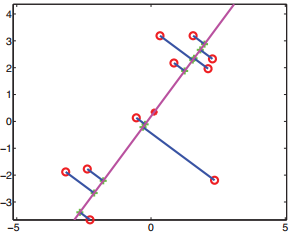
\includegraphics[scale=.60]{PCA-PPCA-a.png}} \\
\subfloat[]{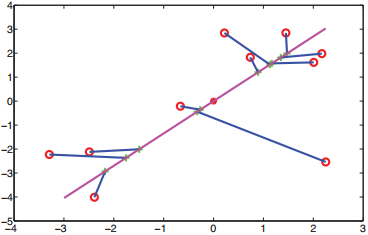
\includegraphics[scale=.60]{PCA-PPCA-b.png}}
\caption{An illustration of PCA and PPCA where $D=2$ and $L=1$. Circles are the original data points, crosses are the reconstructions. The red star is the data mean. (a) PCA. The points are orthogonally projected onto the line. (b) PPCA. The projection is no longer orthogonal: the reconstructions are shrunk towards the data mean (red star).}
\label{fig:PCA-PPCA} 
\end{figure}

The principal directions are the ones along which the data shows maximal variance. This means that PCA can be “misled” by directions in which the variance is high merely because of the measurement scale. It is therefore standard practice to standardize the data first, or equivalently, to work with correlation matrices instead of covariance matrices. 


\subsubsection{Proof *}
See Section 12.2.2 of MLAPP.


\subsection{Singular value decomposition (SVD)}
We have defined the solution to PCA in terms of eigenvectors of the covariance matrix. However, there is another way to obtain the solution, based on the \textbf{singular value decomposition}, or \textbf{SVD}. This basically generalizes the notion of eigenvectors from square matrices to any kind of matrix.

\begin{theorem}(\textbf{SVD}).
Any matrix can be decomposed as follows
\begin{equation}\label{eqn:SVD}
\underbrace{\vec{X}}_{N \times D}=\underbrace{\vec{U}}_{N \times N}\underbrace{\vec{\Sigma}}_{N \times D}\underbrace{\vec{V}^T}_{D \times D}
\end{equation}
where $\vec{U}$ is an $N \times N$ matrix whose columns are orthornormal(so $\vec{U}^T\vec{U}=\vec{I}$), $\vec{V}$ is $D \times D$ matrix whose rows and columns are orthonormal (so $\vec{V}^T\vec{V}=\vec{V}\vec{V}^T=\vec{I}_D$), and $\vec{\Sigma}$ is a $N \times D$ matrix containing the $r=\min(N,D)$ singular values $\sigma_i \geq 0$ on the main diagonal, with 0s filling the rest of the matrix.
\end{theorem}

This shows how to decompose the matrix $X$ into the product of three matrices: $\vec{V}$ describes an orthonormal basis in the domain, and $\vec{U}$ describes an orthonormal basis in the co-domain, and $\vec{\Sigma}$ describes how much the vectors in $\vec{V}$ are stretched to give the vectors in $\vec{U}$.

Since there are at most $D$ singular values (assuming $N>D$), the last $N−D$ columns of $\vec{U}$ are irrelevant, since they will be multiplied by 0. The \textbf{economy sized SVD}, or \textbf{thin SVD}, avoids computing these unnecessary elements. Let us denote this decomposition by $\hat{\vec{U}}\hat{\vec{\Sigma}}\hat{\vec{V}}^T$.If $N>D$, we have
\begin{equation}
\underbrace{\vec{X}}_{N \times D}=\underbrace{\hat{\vec{U}}}_{N \times D}\underbrace{\hat{\vec{\Sigma}}}_{D \times D}\underbrace{\hat{\vec{V}}^T}_{D \times D}
\end{equation}
as in Figure \ref{fig:SVD}(a). If $N<D$, we have
\begin{equation}
\underbrace{\vec{X}}_{N \times D}=\underbrace{\hat{\vec{U}}}_{N \times N}\underbrace{\hat{\vec{\Sigma}}}_{N \times N}\underbrace{\hat{\vec{V}}^T}_{N \times D}
\end{equation}
Computing the economy-sized SVD takes $O(ND\min(N,D))$ time (Golub and van Loan 1996, p254).

\begin{figure}[hbtp]
\centering
\subfloat[]{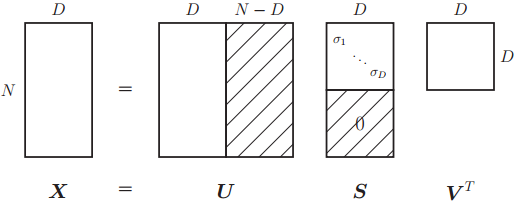
\includegraphics[scale=.50]{SVD-a.png}} \\
\subfloat[]{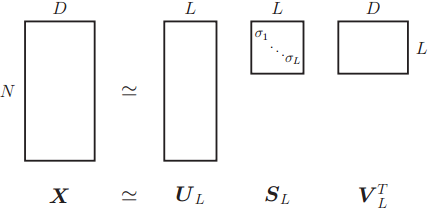
\includegraphics[scale=.50]{SVD-b.png}}
\caption{(a) SVD decomposition of non-square matrices $\vec{X}=\vec{U}\vec{\Sigma}\vec{V}^T$. The shaded parts of $\vec{\Sigma}$, and all the off-diagonal terms, are zero. The shaded entries in $\vec{U}$ and $\vec{\Sigma}$ are not computed in the economy-sized version, since they are not needed. (b) Truncated SVD approximation of rank $L$.}
\label{fig:SVD} 
\end{figure}

The connection between eigenvectors and singular vectors is the following:
\begin{align}
\vec{U}&=\mathrm{evec}(\vec{X}\vec{X}^T) \\
\vec{V}&=\mathrm{evec}(\vec{X}^T\vec{X}) \\
\vec{\Sigma}^2&=\mathrm{eval}(\vec{X}\vec{X}^T)=\mathrm{eval}(\vec{X}^T\vec{X})
\end{align}
For the proof please read Section 12.2.3 of MLAPP.

Since the eigenvectors are unaffected by linear scaling of a matrix, we see that the right singular vectors of $\vec{X}$ are equal to the eigenvectors of the empirical covariance $\hat{\vec{\Sigma}}$. Furthermore, the eigenvalues of $\hat{\vec{\Sigma}}$ are a scaled version of the squared singular values.

However, the connection between PCA and SVD goes deeper. From Equation \ref{eqn:SVD}, we can represent a rank $r$ matrix as follows:
\begin{equation*}
\vec{X}=\sigma_1\left(\begin{array}{c} | \\ \vec{u}_1 \\ | \end{array}\right)\left(\begin{array}{ccc} - & \vec{v}_1 & - \end{array}\right)+\cdots+\sigma_r\left(\begin{array}{c} | \\ \vec{u}_r \\ | \end{array}\right)\left(\begin{array}{ccc} - & \vec{v}_r^T & - \end{array}\right)
\end{equation*}
If the singular values die off quickly, we can produce a rank $L$ approximation to the matrix as follows:
\begin{align}
\vec{X} & \approx \sigma_1\left(\begin{array}{c} | \\ \vec{u}_1 \\ | \end{array}\right)\left(\begin{array}{ccc} - & \vec{v}_1 & - \end{array}\right)+\cdots+\sigma_r\left(\begin{array}{c} | \\ \vec{u}_L \\ | \end{array}\right)\left(\begin{array}{ccc} - & \vec{v}_L^T & - \end{array}\right) \nonumber \\
 & = \vec{U}_{:,1:L}\vec{\Sigma}_{1:L,1:L}\vec{V}_{:,1:L}^T
\end{align}
This is called a \textbf{truncated SVD} (see Figure \ref{fig:SVD}(b)).

One can show that the error in this approximation is given by
\begin{equation}
\lVert \vec{X}-\vec{X}_L \rVert_F \approx \sigma_L
\end{equation}
Furthermore, one can show that the SVD offers the best rank $L$ approximation to a matrix (best in the sense of minimizing the above Frobenius norm).

Let us connect this back to PCA. Let $\vec{X}=\vec{U}\vec{\Sigma}\vec{V}^T$ be a truncated SVD of $\vec{X}$. We know that $\hat{\vec{W}}=\vec{V}$, and that $\hat{\vec{Z}}=\vec{X}\hat{\vec{W}}$, so
\begin{equation}
\hat{\vec{Z}}=\vec{U}\vec{\Sigma}\vec{V}^T\vec{V}=\vec{U}\vec{\Sigma}
\end{equation}
Furthermore, the optimal reconstruction is given by $\hat{\vec{X}}=\vec{Z}\hat{\vec{W}}$,so we find
\begin{equation}
\hat{\vec{X}}=\vec{U}\vec{\Sigma}\vec{V}^T
\end{equation}
This is precisely the same as a truncated SVD approximation! This is another illustration of the fact that PCA is the best low rank approximation to the data.


\subsection{Probabilistic PCA}
\begin{theorem}((\textbf{Tipping and Bishop 1999})).
Consider a factor analysis model in which $\vec{\Psi}=\sigma^2\vec{I}$ and $\vec{W}$ is orthogonal. The observed data log likelihood is given by
\begin{align}
\log p(\vec{X}|\vec{W},\sigma^2\vec{I}) & =-\frac{N}{2}\ln|\vec{C}|-\frac{1}{2}\sum\limits_{i=1}^N \vec{x}_i^T\vec{C}^{-1}\vec{x}_i \nonumber \\
   & =-\frac{N}{2}\ln|\vec{C}|+\mathrm{tr}(\vec{C}^{-1}\vec{\Sigma})
\end{align}
where $\vec{C}=\vec{W}\vec{W}^T+\sigma^2\vec{I}$ and $\vec{\Sigma}=\frac{1}{N}\sum_{i=1}^N \vec{x}_i\vec{x}_i^T=\frac{1}{N}\vec{X}\vec{X}^T$. (We are assuming centred data, for notational simplicity.) The maxima of the log-likelihood are given by
\begin{equation}
\hat{\vec{W}}=\vec{V}(\vec{\Lambda}-\sigma^2\vec{I})^{\frac{1}{2}}\vec{R}
\end{equation}
where $\vec{R}$ is an arbitrary $L \times L$ orthogonal matrix, $\vec{V}$ is the $D \times L$ matrix whose columns are the first $L$ eigenvectors of $\vec{\Sigma}$, and $\vec{\Lambda}$ is the corresponding diagonal matrix of eigenvalues. Without loss of generality, we can set $\vec{R}=\vec{I}$. Furthermore, the MLE of the noise variance is given by
\begin{equation}
\hat{\sigma}^2=\frac{1}{D-L}\sum\limits_{j=L+1}^D \lambda_j
\end{equation}
which is the average variance associated with the discarded dimensions.
\end{theorem}

Thus, as $\sigma^2 \rightarrow 0$, we have $\hat{\vec{W}} \rightarrow \vec{V}$, as in classical PCA. What about $\hat{\vec{Z}}$? It is easy to see that the posterior over the latent factors is given by
\begin{align}
p(\vec{z}_i|\vec{x}_i,\hat{\vec{\theta}}) & = \mathcal{N}(\vec{z}_i|\hat{\vec{F}}^{-1}\hat{\vec{W}}^T\vec{x}_i,\sigma^2\hat{\vec{F}}^{-1}) \label{eqn:PPCA-posterior}\\
\hat{\vec{F}} & \triangleq \hat{\vec{W}}^T\hat{\vec{W}}+\sigma^2\vec{I}
\end{align}
(Do not confuse $\vec{F} = \vec{W}^T\vec{W}+\sigma^2\vec{I}$ with $\vec{C}=\vec{W}\vec{W}^T+\sigma^2\vec{I}$.) Hence, as $\sigma^2 \rightarrow 0$, we find $\hat{\vec{W}} \rightarrow \vec{V}$, $\hat{\vec{F}} \rightarrow \vec{I}$ and $\vec{z}_i \rightarrow \vec{V}^T\vec{x}_i$. Thus the posterior mean is obtained by an orthogonal projection of the data onto the column space of $\vec{V}$, as in classical PCA.

Note, however, that if $\sigma^2 \rightarrow 0$, the posterior mean is not an orthogonal projection, since it is shrunk somewhat towards the prior mean, as illustrated in Figure \ref{fig:PCA-PPCA}(b). This sounds like an undesirable property, but it means that the reconstructions will be closer to the overall data mean, $\hat{\vec{\mu}}=\bar{\vec{x}}$.


\subsection{EM algorithm for PCA}
\label{sec:EM-for-PCA}
Although the usual way to fit a PCA model uses eigenvector methods, or the SVD, we can also use EM, which will turn out to have some advantages that we discuss below. EM for PCA relies on the probabilistic formulation of PCA. However the algorithm continues to work in the zero noise limit, $\sigma^2=0$, as shown by (Roweis 1997).

Let $\tilde{\vec{Z}}$ be a $L \times N$ matrix storing the posterior means (low-dimensional representations) along its columns. Similarly, let $\tilde{\vec{X}}=\vec{X}^T$ store the original data along its columns. From Equation \ref{eqn:PPCA-posterior}, when $\sigma^2=0$, we have
\begin{equation}
\tilde{\vec{Z}}=(\vec{W}^T\vec{W})^{-1}\vec{W}^T\tilde{\vec{X}}
\end{equation}
This constitutes the E step. Notice that this is just an orthogonal projection of the data.

From Equation \ref{eqn:FA-EM-W}, the M step is given by
\begin{equation}
\hat{\vec{W}}=\left(\sum\limits_{i=1}^N \vec{x}_i\mathbb{E}[\vec{z}_i]^T\right)\left(\sum\limits_{i=1}^N \mathbb{E}[\vec{z}_i]\mathbb{E}[\vec{z}_i]^T\right)^{-1}
\end{equation}
where we exploited the fact that $\vec{\Sigma}=\mathrm{cov}[\vec{z}_i|\vec{x}_i,\vec{\theta}]=\vec{0}$ when $\sigma^2=0$.

(Tipping and Bishop 1999) showed that the only stable fixed point of the EM algorithm is the globally optimal solution. That is, the EM algorithm converges to a solution where $\vec{W}$ spans the same linear subspace as that defined by the first $L$ eigenvectors. However, if we want $\vec{W}$ to be orthogonal, and to contain the eigenvectors in descending order of eigenvalue, we have to orthogonalize the resulting matrix (which can be done quite cheaply). Alternatively, we can modify EM to give the principal basis directly (Ahn and Oh 2003).

This algorithm has a simple physical analogy in the case $D=2$ and $L=1$(Roweis 1997). Consider some points in $\mathbb{R}^2$ attached by springs to a rigid rod, whose orientation is defined by a vector $\vec{w}$. Let $\vec{z}_i$ be the location where the $i$'th spring attaches to the rod. See Figure 12.11 of MLAPP for an illustration.

Apart from this pleasing intuitive interpretation, EM for PCA has the following advantages over eigenvector methods:
\begin{itemize}
\item{EM can be faster. In particular, assuming $N,D \gg L$, the dominant cost of EM is the projection operation in the E step, so the overall time is $O(TLND)$, where $T$ is the number of iterations. This is much faster than the $O(\min(ND^2,DN^2))$ time required by straightforward eigenvector methods, although more sophisticated eigenvector methods, such as the Lanczos algorithm, have running times comparable to EM.}
\item{EM can be implemented in an online fashion, i.e., we can update our estimate of $\vec{W}$ as the data streams in.}
\item{EM can handle missing data in a simple way (see Section \ref{sec:Fitting-FA-models-with-missing-data}).}
\item{EM can be extended to handle mixtures of PPCA/ FA models.}
\item{EM can be modified to variational EM or to variational Bayes EM to fit more complex models.}
\end{itemize}


\section{Choosing the number of latent dimensions}
\label{sec:FA-Choosing-L}
In Section \ref{sec:Model-selection-for-LVM}, we discussed how to choose the number of components $K$ in a mixture model. In this section, we discuss how to choose the number of latent dimensions $L$ in a FA/PCA model.


\subsection{Model selection for FA/PPCA}
TODO

\subsection{Model selection for PCA}
TODO



\section{PCA for categorical data}
In this section, we consider extending the factor analysis model to the case where the observed data is categorical rather than real-valued. That is, the data has the form $y_{ij} \in \{1,...,C\}$, where $j=1:R$ is the number of observed response variables. We assume each $y_{ij}$ is generated from a latent variable $\vec{z}_i \in \mathbb{R}^L$, with a Gaussian prior, which is passed through the softmax function as follows:
\begin{align}
p(\vec{z}_i) & = \mathcal{N}(\vec{z}_i|\vec{0},\vec{I}) \\
p(\vec{y}_i|\vec{z}_i,\vec{\theta}) & = \prod\limits_{j=1}^R \mathrm{Cat}(y_{ir}|\mathcal{S}(\vec{W}_r^T\vec{z}_i+\vec{w}_{0r}))
\end{align}
where $\vec{W}_r \in \mathbb{R}^L$ is the factor loading matrix for response $j$, and $\vec{W}_{0r} \in \mathbb{R}^M$ is the offset term for response $r$, and $\vec{\theta}=(\vec{W}_r,\vec{W}_{0r})_{r=1}^R$. (We need an explicit offset term, since clamping one element of $\vec{z}_i$ to 1 can cause problems when computing the posterior covariance.) As in factor analysis, we have defined the prior mean to be $\vec{\mu}_0=\vec{0}$ and the prior covariance $\vec{V}_0=\vec{I}$, since we can capture non-zero mean by changing $\vec{w}_{0j}$ and non-identity covariance by changing $\vec{W}_r$. We will call this categorical PCA. See Chapter 27 TODO for a discussion of related models.

In (Khan et al. 2010), we show that this model outperforms finite mixture models on the task of imputing missing entries in design matrices consisting of real and categorical data. This is useful for analysing social science survey data, which often has missing data and variables of mixed type.


\section{PCA for paired and multi-view data}


\subsection{Supervised PCA (latent factor regression)}


\subsection{Discriminative supervised PCA}


\subsection{Canonical correlation analysis}


\section{Independent Component Analysis (ICA)}
\label{sec:ICA}
Let $\vec{x}_t \in \mathbb{R}^D$ be the observed signal at the sensors at “time” $t$, and $\vec{z}_t \in \mathbb{R}^L$ be the vector of source signals. We assume that
\begin{equation}
\vec{x}_t=\vec{W}\vec{z}_t+\vec{\epsilon}_t
\end{equation}
where $\vec{W}$ is an $D \times L$ matrix, and $\vec{\epsilon}_t \sim \mathcal{N}(\vec{0},\vec{\Psi})$. In this section, we treat each time point as an independent observation, i.e., we do not model temporal correlation (so we could replace the $t$ index with $i$, but we stick with t to be consistent with much of the ICA literature). The goal is to infer the source signals, $p(\vec{z}_t|\vec{x}_t,\vec{\theta})$. In this context, $\vec{W}$ is called the \textbf{mixing matrix}. If $L=D$ (number of sources = number of sensors), it will be a square matrix. Often we will assume the noise level, $|\vec{\Psi}|$, is zero, for simplicity.

So far, the model is identical to factor analysis. However, we will use a different prior for $p(\vec{z}_t)$. In PCA, we assume each source is independent, and has a Gaussian distribution. We will now relax this Gaussian assumption and let the source distributions be any \emph{non-Gaussian} distribution
\begin{equation}
p(\vec{z}_t) =\prod\limits_{j=1}^L p_j(z_{tj})
\end{equation}
Without loss of generality, we can constrain the variance of the source distributions to be \vec{1}, because any other variance can be modelled by scaling the rows of $\vec{W}$ appropriately. The resulting model is known as \textbf{independent component analysis} or \textbf{ICA}.

The reason the Gaussian distribution is disallowed as a source prior in ICA is that it does not permit unique recovery of the sources. This is because the PCA likelihood is invariant to any orthogonal transformation of the sources $\vec{z}_t$ and mixing matrix $\vec{W}$. PCA can recover the best linear subspace in which the signals lie, but cannot uniquely recover the signals themselves.

ICA requires that $\vec{W}$ is square and hence invertible. In the non-square case (e.g., where we have more sources than sensors), we cannot uniquely recover the true signal, but we can compute the posterior $p(\vec{z}_t|\vec{x}_t,\hat{\vec{W}})$, which represents our beliefs about the source. In both cases, we need to estimate Was well as the source distributions $p_j$. We discuss how to do this below.


\subsection{Maximum likelihood estimation}
In this section, we discuss ways to estimate square mixing matrices $\vec{W}$ for the noise-free ICA model. As usual, we will assume that the observations have been centered; hence we can also assume $\vec{z}$ is zero-mean. In addition, we assume the observations have been whitened, which can be done with PCA. 

If the data is centered and whitened, we have $\mathbb{E}[\vec{x}\vec{x}^T]=\vec{I}$. But in the noise free case, we also have
\begin{equation}
\mathrm{cov}[\vec{x}]=\mathbb{E}[\vec{x}\vec{x}^T]=\vec{W}\mathbb{E}[\vec{z}\vec{z}^T]\vec{W}^T
\end{equation}
Hence we see that $\vec{W}$ must be orthogonal. This reduces the number of parameters we have to estimate from $D^2$ to $D(D-1)/2$. It will also simplify the math and the algorithms.

Let $\vec{V}=\vec{W}^{-1}$; these are often called the recognition weights, as opposed to $\vec{W}$, which are the generative weights.

Since $\vec{x}=\vec{W}\vec{z}$, we have, from Equation \ref{eqn:Multivariate-transformation},
\begin{align}
p_x(\vec{W}\vec{z}_t) & =p_z(\vec{z}_t)|\mathrm{det}(\vec{W}^{-1})| \nonumber \\
   & = p_z(\vec{V}\vec{x}_t)|\mathrm{det}(\vec{V})|
\end{align}
Hence we can write the log-likelihood, assuming $T$ iid samples, as follows:
\begin{equation*}
\frac{1}{T} \log p(\mathcal{D}|\vec{V})=\log|\mathrm{det}(\vec{V})|+\frac{1}{T}\sum\limits_{j=1}^L \sum\limits_{t=1}^T \log p_j(\vec{v}_j^T\vec{x}_t)
\end{equation*}
where $\vec{v}_j$ is the $j$'th row of $\vec{V}$. Since we are constraining $\vec{V}$ to be orthogonal, the first term is a constant, so we can drop it. We can also replace the average over the data with an expectation operator to get the following objective
\begin{equation}
\mathrm{NLL}(\vec{V})=\sum\limits_{j=1}^L \mathbb{E}[G_j(\vec{z}_j)]
\end{equation}
where $\vec{z}_j=\vec{v}_j^T\vec{x}$ and $G_j(\vec{z}) \triangleq -\log p_j(\vec{z})$. We want to minimize this subject to the constraint that the rows of $\vec{V}$ are orthogonal. We also want them to be unit norm, since this ensures that the variance of the factors is unity (since, with whitened data, $\mathbb{E}[\vec{v}_j^T\vec{x}]=\lVert \vec{v}_j \rVert^2$, which is necessary to fix the scale of the weights. In otherwords, $\vec{V}$ should be an orthonormal matrix.

It is straightforward to derive a gradient descent algorithm to fit this model; however, it is rather slow. One can also derive a faster algorithm that follows the natural gradient; see e.g., (MacKay 2003, ch 34) for details. A popular alternative is to use an approximate Newton method, which we discuss in Section \ref{sec:FastICA}. Another approach is to use EM, which we discuss in Section \ref{sec:ICA-EM}.


\subsection{The FastICA algorithm}
\label{sec:FastICA}


\subsection{Using EM}
\label{sec:ICA-EM}


\subsection{Other estimation principles *}


%\chapter{Sparse linear models}


%\chapter{Kernels}
\label{chap:Kernels}

\section{Introduction}
So far in this book, we have been assuming that each object that we wish to classify or cluster or process in anyway can be represented as a fixed-size feature vector, typically of the form $\vec{x}_i \in \mathbb{R}^D$. However, for certain kinds of objects, it is not clear how to best represent them as fixed-sized feature vectors. For example, how do we represent a text document or protein sequence, which can be of variable length? or a molecular structure, which has complex 3d geometry? or an evolutionary tree, which has variable size and shape?

One approach to such problems is to define a generative model for the data, and use the inferred latent representation and/or the parameters of the model as features, and then to plug these features in to standard methods. For example, in Chapter 28 TODO, we discuss deep learning, which is essentially an unsupervised way to learn good feature representations.

Another approach is to assume that we have some way of measuring the similarity between objects, that doesn’t require preprocessing them into feature vector format. For example, when comparing strings, we can compute the edit distance between them. Let $\kappa(\vec{x},\vec{x}') \geq 0$ be some measure of similarity between objects $\kappa(\vec{x},\vec{x}') \in \mathcal{X}$,  we will call $\kappa$ a \textbf{kernel function}. Note that the word “kernel” has several meanings; we will discuss a different interpretation in Section 14.7.1 TODO.

In this chapter, we will discuss several kinds of kernel functions. We then describe some algorithms that can be written purely in terms of kernel function computations. Such methods can be used when we don’t have access to (or choose not to look at) the “inside” of the objects $\vec{x}$ that we are processing.


\section{Kernel functions}
\begin{definition}
A \textbf{kernel function}\footnote{\url{http://en.wikipedia.org/wiki/Kernel_function}} is a real-valued function of two arguments, $\kappa(\vec{x},\vec{x}') \in \mathbb{R}$. Typically the function is symmetric (i.e., $\kappa(\vec{x},\vec{x}')=\kappa(\vec{x}',\vec{x})$, and non-negative (i.e., $\kappa(\vec{x},\vec{x}') \geq 0$). 
\end{definition}

We give several examples below.

\subsection{RBF kernels}
The \textbf{Gaussian kernel} or \textbf{squared exponential kernel}(SE kernel) is defined by
\begin{equation}
\kappa(\vec{x},\vec{x}')=\exp\left(-\frac{1}{2}(\vec{x}-\vec{x}')^T\vec{\Sigma}^{-1}(\vec{x}-\vec{x}')\right)
\end{equation}

If $\vec{\Sigma}$ is diagonal, this can be written as
\begin{equation}
\kappa(\vec{x},\vec{x}')=\exp\left(-\frac{1}{2}\sum\limits_{j=1}^D \frac{1}{\sigma_j^2}(x_j-x_j')^2\right)
\end{equation}

We can interpret the $\sigma_j$ as defining the \textbf{characteristic length scale} of dimension $j$.If $\sigma_j = \infty$, the corresponding dimension is ignored; hence this is known as the \textbf{ARD kernel}. If $\vec{\Sigma}$ is spherical, we get the isotropic kernel
\begin{equation}\label{eqn:RBF-kernel}
\kappa(\vec{x},\vec{x}')=\exp\left(-\frac{\lVert\vec{x}-\vec{x}'\rVert^2}{2\sigma^2}\right)
\end{equation}

Here $\sigma^2$ is known as the \textbf{bandwidth}. Equation \ref{eqn:RBF-kernel} is an example of a \textbf{radial basis function} or \textbf{RBF} kernel, since it is only a function of $\lVert\vec{x}-\vec{x}'\rVert^2$.


\subsection{TF-IDF kernels}
\begin{equation}\label{eqn:RBF-kernel}
\kappa(\vec{x},\vec{x}')=\frac{\phi(\vec{x})^T\phi(\vec{x}')}{\lVert\phi(vec{x})\rVert_2\lVert\phi(\vec{x}')\rVert_2}
\end{equation}
where $\phi(\vec{x})=\text{tf-idf}(\vec{x})$.

\subsection{Mercer (positive definite) kernels}
\label{sec:Mercer-kernels}
If the kernel function satisfies the requirement that the \textbf{Gram matrix}, defined by
\begin{equation}
\vec{K} \triangleq \left(\begin{array}{ccc}
\kappa(\vec{x}_1,\vec{x}_2) & \cdots \kappa(\vec{x}_1,\vec{x}_N) \\
\vdots & \vdots & \vdots \\
\kappa(\vec{x}_N,\vec{x}_1) & \cdots \kappa(\vec{x}_N,\vec{x}_N) 
\end{array}\right)
\end{equation}
be positive definite for any set of inputs $\{\vec{x}_i\}_{i=1}^N$. We call such a kernel a \textbf{Mercer kernel},or \textbf{positive definite kernel}.

If the Gram matrix is positive definite, we can compute an eigenvector decomposition of it as follows
\begin{equation}
\vec{K}=\vec{U}^T\vec{\Lambda}\vec{U}
\end{equation}

where $\vec{\Lambda}$ is a diagonal matrix of eigenvalues $\lambda_i >0$. Now consider an element of $\vec{K}$:
\begin{equation}
k_{ij}=(\vec{\Lambda}^{\frac{1}{2}}\vec{U}_{:,i})^T(\vec{\Lambda}^{\frac{1}{2}}\vec{U}_{:,j})
\end{equation}

Let us define $\phi(\vec{x}_i)=\vec{\Lambda}^{\frac{1}{2}}\vec{U}_{:,i}$, then we can write
\begin{equation}
k_{ij}=\phi(\vec{x}_i)^T\phi(\vec{x}_j)
\end{equation}

Thus we see that the entries in the kernel matrix can be computed by performing an inner product of some feature vectors that are implicitly defined by the eigenvectors $\vec{U}$. In general, if the kernel is Mercer, then there exists a function $\phi$ mapping $\vec{x} \in \mathcal{X}$ to $\mathbb{R}^D$ such that
\begin{equation}
\kappa(\vec{x},\vec{x}')=\phi(\vec{x})^T\phi(\vec{x}')
\end{equation}
where $\phi$ depends on the eigen functions of $\kappa$(so $D$ is a potentially infinite dimensional space).

For example, consider the (non-stationary) \textbf{polynomial kernel} $\kappa(\vec{x},\vec{x}')=(\gamma \vec{x}\vec{x}'+r)^M$, where $r>0$. One can show that the corresponding feature vector $\phi(\vec{x})$ will contain all terms up to degree $M$. For example, if $M=2, \gamma=r=1$ and $\vec{x}, \vec{x}' \in \mathbb{R}^2$, we have
\begin{align*}
(\vec{x}\vec{x}'+1)^2 & =(1+x_1x_1'+x_2+x_2')^2 \\
    & = 1+2x_1x_1'+2x_2x_2'+(x_1x_1')^2+(x_2x_2')^2x_1x_1'x_2x_2' \\
	& = \phi(\vec{x})^T\phi(\vec{x}') \\
\text{where } & \phi(\vec{x})=(1,\sqrt{2}x_1,\sqrt{2}x_2,x_1^2,x_2^2,\sqrt{2}x_1x_2)
\end{align*}

In the case of a Gaussian kernel, the feature map lives in an infinite dimensional space. In such a case, it is clearly infeasible to explicitly represent the feature vectors.

In general, establishing that a kernel is a Mercer kernel is difficult, and requires techniques from functional analysis. However, one can show that it is possible to build up new Mercer kernels from simpler ones using a set of standard rules. For example, if $\kappa_1$ and $\kappa_2$ are both Mercer, so is $\kappa(\vec{x},\vec{x}')=\kappa_1(\vec{x},\vec{x}')+\kappa_2(\vec{x},\vec{x}')=$. See e.g., (Schoelkopf and Smola 2002) for details.


\subsection{Linear kernels}
\begin{equation}
\kappa(\vec{x},\vec{x}')=\vec{x}^T\vec{x}'
\end{equation}

\subsection{Matern kernels}
The \textbf{Matern kernel}, which is commonly used in Gaussian process regression (see Section 15.2), has the following form
\begin{equation}
\kappa(r)=\frac{2^{1-\nu}}{\Gamma(\nu)}\left(\frac{\sqrt{2\nu}r}{\ell}\right)^{\nu}K_{\nu}\frac{\sqrt{2\nu}r}{\ell}
\end{equation}
where $r=\lVert\vec{x}-\vec{x}'\rVert$, $\nu>0$, $\ell>0$, and $K_{\nu}$ is a modified Bessel function. As $\nu \rightarrow \infty$, this approaches the SE kernel. If $\nu=\frac{1}{2}$, the kernel simplifies to
\begin{equation}
\kappa(r)=\exp(-r/\ell)
\end{equation}

If $D=1$, and we use this kernel to define a Gaussian process (see Chapter 15 TODO), we get the \textbf{Ornstein-Uhlenbeck process}, which describes the velocity of a particle undergoing Brownian motion (the corresponding function is continuous but not differentiable, and hence is very “jagged”).


\subsection{String kernels}
\label{sec:String-kernels}
Now let $\phi_s(\vec{x})$ denote the number of times that substrings appears in string $\vec{x}$. We define the kernel between two strings $\vec{x}$ and $\vec{x}'$ as
\begin{equation}
\kappa(\vec{x},\vec{x}')=\sum\limits_{s \in \mathcal{A}^*} w_s\phi_s(\vec{x})\phi_s(\vec{x}')
\end{equation}
where $w_s \geq 0$ and $\mathcal{A}^*$ is the set of all strings (of any length) from the alphabet $\mathcal{A}$(this is known as the Kleene star operator). This is a Mercer kernel, and be computed in $O(|\vec{x}|+|\vec{x}'|)$ time (for certain settings of the weights $\{ws\}$) using suffix trees (Leslie et al. 2003; Vishwanathan and Smola 2003; Shawe-Taylor and Cristianini 2004).

There are various cases of interest. If we set $w_s =0$for $|s| >1$ we get a bag-of-characters kernel. This defines $\phi(\vec{x})$ to be the number of times each character in $\mathcal{A}$ occurs in $\vec{x}$.If we require $s$ to be bordered by white-space, we get a bag-of-words kernel, where $\phi(\vec{x})$ counts how many times each possible word occurs. Note that this is a very sparse vector, since most words will not be present. If we only consider strings of a fixed lengthk, we get the \textbf{k-spectrum} kernel. This has been used to classify proteins into SCOP superfamilies (Leslie et al. 2003).


\subsection{Pyramid match kernels}
% \begin{figure}[hbtp]
% \centering
%     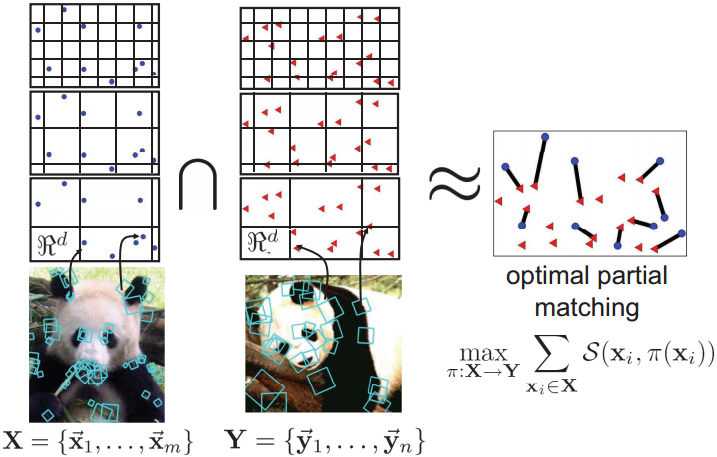
\includegraphics[scale=.70]{pyramid-match-kernel.png}
% \caption{Illustration of a pyramid match kernel computed from two images. Used with kind permission of Kristen Grauman.}
% \label{fig:pyramid-match-kernel}
% \end{figure}


\subsection{Kernels derived from probabilistic generative models}
Suppose we have a probabilistic generative model of feature vectors, $p(\vec{x}|\vec{\theta})$. Then there are several ways we can use this model to define kernel functions, and thereby make the model suitable for discriminative tasks. We sketch two approaches below.


\subsubsection{Probability product kernels}
\begin{equation}\label{eqn:Probability-product-kernels}
\kappa(\vec{x}_i,\vec{x}_j)=\int p(\vec{x}|\vec{x}_i)^{\rho}p(\vec{x}|\vec{x}_j)^{\rho}\mathrm{d}\vec{x}
\end{equation}
where $\rho>0$, and $p(\vec{x}|\vec{x}_i)$ is often approximated by $p(\vec{x}|\hat{\vec{\theta}}(\vec{x}_i))$,where $\hat{\vec{\theta}}(\vec{x}_i)$ is a parameter estimate computed using a single data vector. This is called a \textbf{probability product kernel}(Jebara et al. 2004).

Although it seems strange to fit a model to a single data point, it is important to bear in mind that the fitted model is only being used to see how similar two objects are. In particular, if we fit the model to $\vec{x}_i$ and then the model thinks $\vec{x}_j$ is likely, this means that $\vec{x}_i$ and $\vec{x}_j$ are similar. For example, suppose $p(\vec{x}|\vec{\theta}) \sim \mathcal{N}(\vec{\mu},\sigma^2\vec{I})$, where $\sigma^2$ is fixed. If $\rho=1$, and we use $\hat{\vec{\mu}}(\vec{x}_i)=\vec{x}_i$ and $\hat{\vec{\mu}}(\vec{x}_j)=\vec{x}_j$, we find (Jebara et al. 2004, p825) that
\begin{equation}
\kappa(\vec{x}_i,\vec{x}_j)=\frac{1}{(4\pi\sigma^2)^{D/2}}\exp\left(-\frac{1}{4\sigma^2}\lVert\vec{x}_i-\vec{x}_j\rVert^2\right)
\end{equation}
which is (up to a constant factor) the RBF kernel.

It turns out that one can compute Equation \ref{eqn:Probability-product-kernels} for a variety of generative models, including ones with latent variables, such as HMMs. This provides one way to define kernels on variable length sequences. Furthermore, this technique works even if the sequences are of real-valued vectors, unlike the string kernel in Section \ref{sec:String-kernels}. See (Jebara et al. 2004) for further details


\subsubsection{Fisher kernels}
A more efficient way to use generative models to define kernels is to use a \textbf{Fisher kernel} (Jaakkola and Haussler 1998) which is defined as follows:
\begin{equation}
\kappa(\vec{x}_i,\vec{x}_j)=g(\vec{x}_i)^T\vec{F}^{-1}g(\vec{x}_j)
\end{equation}
where $g$ is the gradient of the log likelihood, or \textbf{score vector}, evaluated at the MLE $\hat{\vec{\theta}}$
\begin{equation}
g(\vec{x}) \triangleq \frac{\mathrm{d}}{\mathrm{d}\vec{\theta}}\log p(\vec{x}|\vec{\theta})|_{\hat{\vec{\theta}}}
\end{equation}
and $\vec{F}$ is the Fisher information matrix, which is essentially the Hessian:
\begin{equation}
\vec{F} \triangleq \left[\frac{\partial^2}{\partial \theta_i \partial \theta_j}\log p(\vec{x}|\vec{\theta})\right]|_{\hat{\vec{\theta}}}
\end{equation}

Note that $\hat{\vec{\theta}}$ is a function of all the data, so the similarity of $\vec{x}_i$ and $\vec{x}_j$ is computed in the context of all the data as well. Also, note that we only have to fit one model.


\section{Using kernels inside GLMs}


\subsection{Kernel machines}
We define a \textbf{kernel machine} to be a GLM where the input feature vector has the form
\begin{equation}\label{eqn:kernel-machine}
\phi(\vec{x})=(\kappa(\vec{x},\vec{\mu}_1),\cdots,\kappa(\vec{x},\vec{\mu}_K))
\end{equation}

where $\vec{\mu}_k \in \mathcal{X}$ are a set of $K$ centroids. If $\kappa$ is an RBF kernel, this is called an \textbf{RBF network}. We discuss ways to choose the $\vec{\mu}_k$ parameters below. We will call Equation \ref{eqn:kernel-machine} a \textbf{kernelised feature vector}. Note that in this approach, the kernel need not be a Mercer kernel.

We can use the kernelized feature vector for logistic regression by defining $p(y|\vec{x},\vec{\theta})=\mathrm{Ber}(y|\vec{w}^T\phi(\vec{x}))$. This provides a simple way to define a non-linear decision boundary. For example, see Figure \ref{fig:kenel-machine-xor}.

\begin{figure}[hbtp]
\centering
\subfloat[]{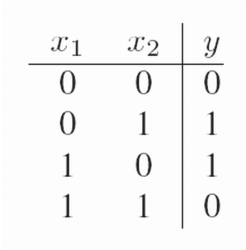
\includegraphics[scale=.70]{kenel-machine-xor-a.png}} \\
\subfloat[]{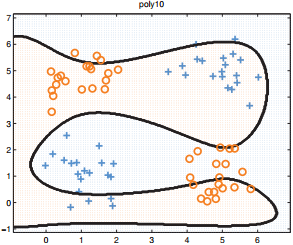
\includegraphics[scale=.70]{kenel-machine-xor-b.png}} \\
\subfloat[]{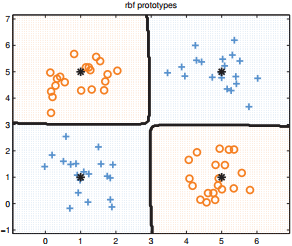
\includegraphics[scale=.70]{kenel-machine-xor-c.png}}
\caption{(a) xor truth table. (b) Fitting a linear logistic regression classifier using degree 10 polynomial expansion. (c) Same model, but using an RBF kernel with centroids specified by the 4 black crosses.}
\label{fig:kenel-machine-xor} 
\end{figure}

We can also use the kernelized feature vector inside a linear regression model by defining $p(y|\vec{x},\vec{\theta})=\mathcal{N}(y|\vec{w}^T\phi(\vec{x}),\sigma^2)$. 


\subsection{L1VMs, RVMs, and other sparse vector machines}
\label{sec:sparse-kernel-machines}
The main issue with kernel machines is: how do we choose the centroids $\vec{\mu}_k$? We can use \textbf{sparse vector machine}, \textbf{L1VM}, \textbf{L2VM}, \textbf{RVM}, \textbf{SVM}.

% In Figure \ref{fig:L2VM-L1VM-RVM-SVM-2d}, we compare L2VM, L1VM, RVM and an SVM using the same RBF kernel on a binary classification problem in 2d.

% \begin{figure}[hbtp]
% \centering
% \subfloat[]{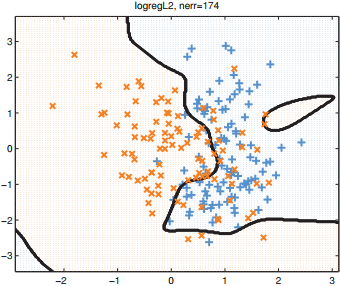
\includegraphics[scale=.50]{L2VM-L1VM-RVM-SVM-2d-a.png}} \\
% \subfloat[]{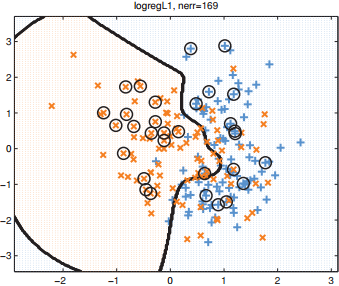
\includegraphics[scale=.50]{L2VM-L1VM-RVM-SVM-2d-b.png}} \\
% \subfloat[]{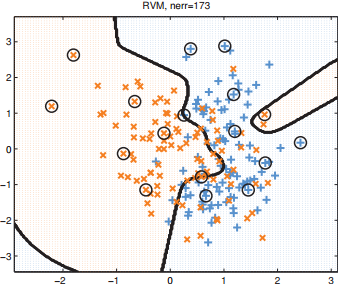
\includegraphics[scale=.50]{L2VM-L1VM-RVM-SVM-2d-c.png}} \\
% \subfloat[]{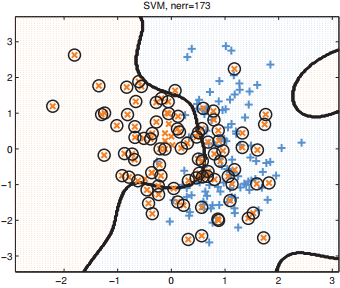
\includegraphics[scale=.50]{L2VM-L1VM-RVM-SVM-2d-d.png}}
% \caption{Example of non-linear binary classification using an RBF kernel with bandwidth $\sigma=0.3$. (a) L2VM with $\lambda=5$. (b) L1VM with $\lambda=1$. (c) RVM. (d) SVM with $C=1/\lambda$ chosen by cross validation. Black circles denote the support vectors.}
% \label{fig:L2VM-L1VM-RVM-SVM-2d} 
% \end{figure}

% In Figure \ref{fig:L2VM-L1VM-RVM-SVM-1d}, we compare L2VM, L1VM, RVM and an SVM using an RBF kernel on a 1d regression problem. 
% \begin{figure}[hbtp]
% \centering
%     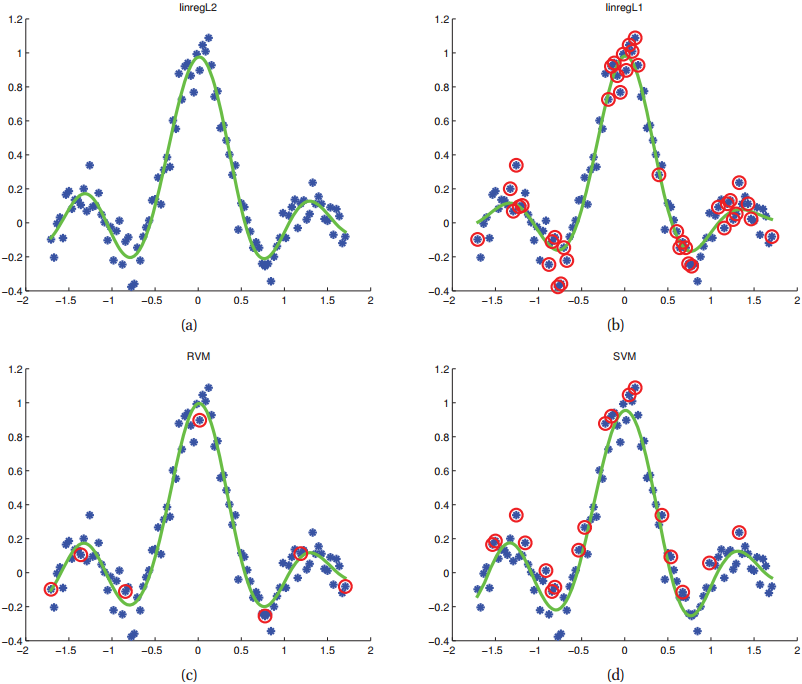
\includegraphics[scale=.70]{L2VM-L1VM-RVM-SVM-1d.png}
% \caption{Example of kernel based regression on the noisy sinc function using an RBF kernel with bandwidth $\sigma=0.3$. (a) L2VM with $\lambda=0.5$. (b) L1VM with $\lambda=0.5$. (c) RVM. (d) SVM regression with $C=1/\lambda$ chosen by cross validation, and $\epsilon=0.1$ (the default for SVMlight). Red circles denote the retained training exemplars.}
% \label{fig:L2VM-L1VM-RVM-SVM-1d} 
% \end{figure}


\section{The kernel trick}
Rather than defining our feature vector in terms of kernels, $\phi(\vec{x})=(\kappa(\vec{x},\vec{x}_1),\cdots,\kappa(\vec{x},\vec{x}_N))$, we can instead work with the original feature vectors $\vec{x}$, but modify the algorithm so that it replaces all inner products of the form $<\vec{x}_i,\vec{x}_j>$ with a call to the kernel function, $\kappa(\vec{x}_i,\vec{x}_j)$. This is called the \textbf{kernel trick}. It turns out that many algorithms can be kernelized in this way. We give some examples below. Note that we require that the kernel be a Mercer kernel for this trick to work.


\subsection{Kernelized KNN}
The Euclidean distance can be unrolled as
\begin{equation}\label{eqn:Euclidean-distance}
\lVert\vec{x}_i-\vec{x}_j\rVert=<\vec{x}_i,\vec{x}_i>+<\vec{x}_j,\vec{x}_j>-2<\vec{x}_i,\vec{x}_j>
\end{equation}
then by replacing all $<\vec{x}_i,\vec{x}_j>$ with $\kappa(\vec{x}_i,\vec{x}_j)$ we get Kernelized KNN.


\subsection{Kernelized K-medoids clustering}
\textbf{K-medoids algorothm} is similar to K-means(see Section \ref{sec:K-means}), but instead of representing each cluster’s centroid by the mean of all data vectors assigned to this cluster, we make each centroid be one of the data vectors themselves. Thus we always deal with integer indexes, rather than data objects.

This algorithm can be kernelized by using Equation \ref{eqn:Euclidean-distance} to replace the distance computation.


\subsection{Kernelized ridge regression}
Applying the kernel trick to distance-based methods was straightforward. It is not so obvious how to apply it to parametric models such as ridge regression. However, it can be done, as we now explain. This will serve as a good “warm up” for studying SVMs.


\subsubsection{The primal problem}
we rewrite Equation \ref{eqn:Ridge-regression-J} as the following
\begin{equation}\label{eqn:Ridge-regression-primal-form}
J(\vec{w})=(\vec{y}-\vec{X}\vec{w})^T(\vec{y}-\vec{X}\vec{w})+\lambda\lVert\vec{w}\rVert^2
\end{equation}
and its solution is given by Equation \ref{eqn:Ridge-regression-solution}.


\subsubsection{The dual problem}
Equation \ref{eqn:Ridge-regression-primal-form} is not yet in the form of inner products. However, using the matrix inversion lemma (Equation 4.107 TODO) we rewrite the ridge estimate as follows
\begin{equation}
\vec{w}=\vec{X}^T(\vec{X}\vec{X}^T+\lambda\vec{I}_N)^{-1}\vec{y}
\end{equation}
which takes $O(N^3+N^2D)$ time to compute. This can be advantageous if $D$ is large. Furthermore, we see that we can partially kernelize this, by replacing $\vec{X}\vec{X}^T$ with the Gram matrix $\vec{K}$. But what about the leading $\vec{X}^T$ term?

Let us define the following \textbf{dual variables}:
\begin{equation}
\vec{\alpha}=(\vec{K}+\lambda\vec{I}_N)^{-1}\vec{y}
\end{equation}

Then we can rewrite the \textbf{primal variables} as follows
\begin{equation}
\vec{w}=\vec{X}^T\vec{\alpha}=\sum\limits_{i=1}^N \alpha_i\vec{x}_i
\end{equation}

This tells us that the solution vector is just a linear sum of the $N$ training vectors. When we plug this in at test time to compute the predictive mean, we get
\begin{equation}
y=f(\vec{x})=\sum\limits_{i=1}^N \alpha_i\vec{x}_i^T\vec{x}=\sum\limits_{i=1}^N \alpha_i\kappa(\vec{x}_i,\vec{x})
\end{equation}

So we have succesfully kernelized ridge regression by changing from primal to dual variables. This technique can be applied to many other linear models, such as logistic regression.


\subsubsection{Computational cost}
The cost of computing the dual variables $\vec{\alpha}$ is $O(N^3)$, whereas the cost of computing the primal variables $\vec{w}$ is $O(D^3)$. Hence the kernel method can be useful in high dimensional settings, even if we only use a linear kernel (c.f., the SVD trick in Equation \ref{eqn:Ridge-regression-SVD}). However, prediction using the dual variables takes $O(ND)$ time, while prediction using the primal variables only takes $O(D)$ time. We can speedup prediction by making $\vec{\alpha}$ sparse, as we discuss in Section \ref{sec:SVMs}.


\subsection{Kernel PCA}
TODO


\section{Support vector machines (SVMs)}
\label{sec:SVMs}
In Section \ref{sec:sparse-kernel-machines}, we saw one way to derive a sparse kernel machine, namely by using a GLM with kernel basis functions, plus a sparsity-promoting prior such as $\ell_1$ or ARD. An alternative approach is to change the objective function from negative log likelihood to some other loss function, as we discussed in Section \ref{sec:Surrogate-loss-functions}. In particular, consider the $\ell_2$ regularized empirical risk function
\begin{equation}
J(\vec{w}, \lambda)=\sum\limits{i=1}^N L(y_i, \hat{y_i})+\lambda\lVert\vec{w}\rVert^2
\end{equation}
where $\hat{y_i}=\vec{w}^T\vec{x}_i+w_0$.

If $L$ is quadratic loss, this is equivalent to ridge regression, and if $L$ is the log-loss defined in Equation \ref{eqn:log-loss}, this is equivalent to logistic regression.

However, if we replace the loss function with some other loss function, to be explained below, we can ensure that the solution is sparse, so that predictions only depend on a subset of the training data, known as \textbf{support vectors}. This combination of the kernel trick plus a modified loss function is known as a \textbf{support vector machine} or \textbf{SVM}. 

Note that SVMs are very unnatural from a probabilistic point of view. 
\begin{itemize}
\item{First, they encode sparsity in the loss function rather than the prior.}
\item{Second, they encode kernels by using an algorithmic trick, rather than being an explicit part of the model. }
\item{Finally, SVMs do not result in probabilistic outputs, which causes various difficulties, especially in the multi-class classification setting (see Section 14.5.2.4 TODO for details).}
\end{itemize}

It is possible to obtain sparse, probabilistic, multi-class kernel-based classifiers, which work as well or better than SVMs, using techniques such as the L1VM or RVM, discussed in Section \ref{sec:sparse-kernel-machines}. However, we include a discussion of SVMs, despite their non-probabilistic nature, for two main reasons. 
\begin{itemize}
\item{First, they are very popular and widely used, so all students of machine learning should know about them.}
\item{Second, they have some computational advantages over probabilistic methods in the structured output case; see Section 19.7 TODO.}
\end{itemize}


\subsection{SVMs for classification}


\subsubsection{Primal form}
\textbf{Representation}
\begin{equation}
\mathcal{H}:y=f(\vec{x})=\text{sign}(\vec{w}\vec{x}+b)
\end{equation}

\textbf{Evaluation}
\begin{eqnarray}
\min_{\vec{w},b}  && \frac{1}{2}\|\vec{w}\|^2 \\
       & s.t. \quad & y_i(\vec{w}\vec{x}_i+b)\geqslant 1, i=1,2, \dots , N
\end{eqnarray}


\subsubsection{Dual form}
\textbf{Representation}
\begin{equation}
\mathcal{H}:y=f(\vec{x})=\text{sign}\left(\sum\limits_{i=1}^N{\alpha_iy_i(\vec{x} \cdot \vec{x}_i)}+b\right)
\end{equation}

\textbf{Evaluation}
\begin{eqnarray}
 \min_{\alpha} && \frac{1}{2} \sum\limits_{i=1}^N\sum\limits_{j=1}^N \alpha_i\alpha_j y_i y_j (\vec{x}_i \cdot \vec{x}_j) - \sum\limits_{i=1}^N \alpha_i \\
               & s.t.  \quad &\sum\limits_{i=1}^N\alpha_i y_i=0 \\
               && \alpha_i \geqslant 0, i=1,2, \dots, N
\end{eqnarray}


\subsubsection{Primal form with slack variables}
\textbf{Representation}
\begin{equation}
\mathcal{H}:y=f(\vec{x})=\text{sign}(\vec{w}\vec{x}+b)
\end{equation}

\textbf{Evaluation}
\begin{eqnarray}
\min_{\vec{w},b}  &&  C \sum\limits_{i=1}^N\xi_i + \frac{1}{2}\|\vec{w}\|^2 \label{eqn:pfwr1} \\
      & s.t. \quad & y_i(\vec{w}\vec{x}_i+b)\geqslant 1-\xi_i  \label{eqn:pfwr2} \\
                  && \xi_i \geqslant 0, \quad i=1,2, \dots, N \label{eqn:pfwr3}
\end{eqnarray}


\subsubsection{Dual form with slack variables}
\textbf{Representation}
\begin{equation}
\mathcal{H}:y=f(\vec{x})=\text{sign}\left(\sum\limits_{i=1}^N{\alpha_iy_i(\vec{x} \cdot \vec{x}_i)}+b\right)
\end{equation}

\textbf{Evaluation}
\begin{eqnarray}
 \min_{\alpha} && \frac{1}{2} \sum\limits_{i=1}^N\sum\limits_{j=1}^N \alpha_i\alpha_j y_i y_j (\vec{x}_i \cdot \vec{x}_j) - \sum\limits_{i=1}^N \alpha_i \\
               & s.t.  \quad & \sum\limits_{i=1}^N\alpha_i y_i=0 \\
               && 0 \leqslant  \alpha_i \leqslant C, i=1,2, \dots, N
\end{eqnarray}

\begin{eqnarray}
\alpha_i=0 \Rightarrow y_i(\vec{w} \cdot \vec{x}_i+b)\geqslant 1 \\
\alpha_i=C \Rightarrow y_i(\vec{w} \cdot \vec{x}_i+b)\leqslant 1 \\
0<\alpha_i<C \Rightarrow y_i(\vec{w} \cdot \vec{x}_i+b)= 1
\end{eqnarray}


\subsubsection{Hinge Loss}
Linear support vector machines can also be interpreted as hinge loss minimization:
\begin{equation}\label{eqn:Hinge-Loss-objective}
\min_{\vec{w},b} \sum\limits_{i=1}^N{L(y_i,f(\vec{x}_i))} + \lambda\|\vec{w}\|^2
\end{equation}
where $L(y, f(\vec{x}))$ is a \textbf{hinge loss function}:
\begin{equation}
L(y, f(\vec{x})) = \begin{cases}
1-yf(x),  & 1-yf(x) > 0 \\
0,  & 1-yf(x) \leqslant 0
\end{cases}
\end{equation}

\begin{proof}
We can write equation \ref{eqn:Hinge-Loss-objective} as equations \ref{eqn:pfwr1} $\sim$ \ref{eqn:pfwr3}.

Define slack variables
\begin{equation}
\xi_i \triangleq 1-y_i(\vec{w} \cdot \vec{x}_i + b),\xi_i \geqslant 0
\end{equation}

Then $\vec{w},b,\xi_i$ satisfy the constraints \ref{eqn:pfwr1} and \ref{eqn:pfwr2}. And objective function \ref{eqn:pfwr3} can be written as
\begin{equation}
\min_{\vec{w},b} \sum\limits_{i=1}^N{\xi_i}+ \lambda\|\vec{w}\|^2 \nonumber
\end{equation}

If $\lambda=\dfrac{1}{2C}$, then 
\begin{equation}
\min_{\vec{w},b} \dfrac{1}{C}\left(C\sum\limits_{i=1}^N{\xi_i}+\dfrac{1}{2}\|\vec{w}\|^2\right)
\end{equation}
It is equivalent to equation \ref{eqn:pfwr1}.

\end{proof}


\subsubsection{Optimization}
QP, SMO


\subsection{SVMs for regression}


\subsubsection{Representation}
\begin{equation}
\mathcal{H}: y=f(\vec{x})=\vec{w}^T\vec{x}+b
\end{equation}


\subsubsection{Evaluation}
\begin{equation}
J(\vec{w})=C\sum\limits_{i=1}^N L(y_i,f(\vec{x}_i))++\dfrac{1}{2}\lVert\vec{w}\rVert^2
\end{equation}
where $L(y,f(\vec{x}))$ is a \textbf{epsilon insensitive loss function}:
\begin{equation}
L(y,f(\vec{x})) = \begin{cases}
0  & , |y-f(\vec{x})|<\epsilon \\
|y-f(\vec{x})|-\epsilon  & , \text{ otherwise}
\end{cases}
\end{equation}
and $C=1/\lambda$ is a regularization constant. 

This objective is convex and unconstrained, but not differentiable, because of the absolute value function in the loss term. As in Section 13.4 TODO, where we discussed the lasso problem, there are several possible algorithms we could use. One popular approach is to formulate the problem as a constrained optimization problem. In particular, we introduce \textbf{slack variables} to represent the degree to which each point lies outside the tube:
\begin{align*}
y_i \leq & f(\vec{x}_i)+\epsilon+\xi_i^+ \\
y_i \geq & f(\vec{x}_i)-\epsilon-\xi_i^- 
\end{align*}

Given this, we can rewrite the objective as follows:
\begin{equation}
J(\vec{w})=C\sum\limits_{i=1}^N (\xi_i^+ + \xi_i^-)++\dfrac{1}{2}\lVert\vec{w}\rVert^2
\end{equation}
This is a standard quadratic problem in $2N+D+1$ variables.


\subsection{Choosing $C$}
\label{sec:SVM-Choosing-C}
SVMs for both classification and regression require that you specify the kernel function and the parameter $C$. Typically $C$ is chosen by cross-validation. Note, however, that $C$ interacts quite strongly with the kernel parameters. For example, suppose we are using an RBF kernel with precision $\gamma=\frac{1}{2\sigma^2}$. If $\gamma=5$, corresponding to narrow kernels, we need heavy regularization, and hence small $C$(so $\lambda=1/C$is big). If $\gamma=1$, a larger value of $C$should be used. So we see that $\gamma$ and $C$ are tightly coupled. This is illustrated in Figure \ref{fig:choosing-C}, which shows the CV estimate of the 0-1 risk as a function of $C$ and $\gamma$.

\begin{figure}[hbtp]
\centering
\subfloat[]{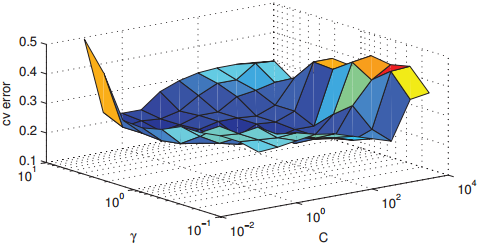
\includegraphics[scale=.50]{choosing-C-a.png}} \\
\subfloat[]{\includegraphics[scale=.50]{choosing-C-b.png}}
\caption{(a) A cross validation estimate of the 0-1 error for an SVM classifier with RBF kernel with different precisions $\gamma=1/(2\sigma^2)$ and different regularizer $\gamma=1/C$, applied to a synthetic data set drawn from a mixture of 2 Gaussians. (b) A slice through this surface for $\gamma=5$ The red dotted line is the Bayes optimal error, computed using Bayes rule applied to the model used to generate the data. Based on Figure 12.6 of (Hastie et al. 2009). }
\label{fig:choosing-C} 
\end{figure}

The authors of libsvm recommend (Hsu et al. 2009) using CV over a 2d grid with values $C \in \{2^{−5},2^{−3},\cdots,2^{15}\}$ and $\gamma \in \{2^{−15},2^{−13},\cdots,2^3\}$. In addition, it is important to standardize the data first, for a spherical Gaussian kernel to make sense.

To choose $C$ efficiently, one can develop a path following algorithm in the spirit of lars (Section 13.3.4 TODO). The basic idea is to start with $\lambda$ large, so that the margin $1/\lVert\vec{w}(\lambda)\rVert$ is wide, and hence all points are inside of it and have $\alpha_i =1$. By slowly decreasing $\lambda$, a small set of points will move from inside the margin to outside, and their $\alpha_i$ values will change from 1 to 0, as they cease to be support vectors. When $\lambda$ is maximal, the function is completely smoothed, and no support vectors remain. See (Hastie et al. 2004) for the details.


\subsection{A probabilistic interpretation of SVMs}
TODO see MLAPP Section 14.5.5


\subsection{Summary of key points}
Summarizing the above discussion, we recognize that SVM classifiers involve three key ingredients: the kernel trick, sparsity, and the large margin principle. The kernel trick is necessary to prevent underfitting, i.e., to ensure that the feature vector is sufficiently rich that a linear classifier can separate the data. (Recall from Section \ref{sec:Mercer-kernels} that any Mercer kernel can be viewed as implicitly defining a potentially high dimensional feature vector.) If the original features are already high dimensional (as in many gene expression and text classification problems), it suffices to use a linear kernel, $\kappa(\vec{x},\vec{x}')=\vec{x}^T\vec{x}'$ , which is equivalent to working with the original features.

The sparsity and large margin principles are necessary to prevent overfitting, i.e., to ensure that we do not use all the basis functions. These two ideas are closely related to each other, and both arise (in this case) from the use of the hinge loss function. However, there are other methods of achieving sparsity (such as $\ell_1$), and also other methods of maximizing the margin(such as boosting). A deeper discussion of this point takes us outside of the scope of this book. See e.g., (Hastie et al. 2009) for more information.


\section{Comparison of discriminative kernel methods}
We have mentioned several different methods for classification and regression based on kernels, which we summarize in Table \ref{tab:Comparison-of-kernel-based-classifiers}. (GP stands for “Gaussian process”, which we discuss in Chapter 15 TODO.) The columns have the following meaning:
\begin{itemize}
\item{Optimize $\vec{w}$: a key question is whether the objective $J(\vec{w}=-\log p(\mathcal{D}|\vec{w})-\log p(\vec{w}))$ is convex or not. L2VM, L1VM and SVMs have convex objectives. RVMs do not. GPs are Bayesian methods that do not perform parameter estimation.}
\item{Optimize kernel: all the methods require that one “tune” the kernel parameters, such as the bandwidth of the RBF kernel, as well as the level of regularization. For methods based on Gaussians, including L2VM, RVMs and GPs, we can use efficient gradient based optimizers to maximize the marginal likelihood. For SVMs, and L1VM, we must use cross validation, which is slower (see Section \ref{sec:SVM-Choosing-C}).}
\item{Sparse: L1VM, RVMs and SVMs are sparse kernel methods, in that they only use a subset of the training examples. GPs and L2VM are not sparse: they use all the training examples. The principle advantage of sparsity is that prediction at test time is usually faster. In addition, one can sometimes get improved accuracy.}
\item{Probabilistic: All the methods except for SVMs produce probabilistic output of the form $p(y|\vec{x})$. SVMs produce a “confidence” value that can be converted to a probability, but such probabilities are usually very poorly calibrated (see Section 14.5.2.3 TODO).}
\item{Multiclass: All the methods except for SVMs naturally work in the multiclass setting, by using a multinoulli output instead of Bernoulli. The SVM can be made into a multiclass classifier, but there are various difficulties with this approach, as discussed in Section 14.5.2.4 TODO.}
\item{Mercer kernel: SVMs and GPs require that the kernel is positive definite; the other techniques do not.}
\end{itemize}

\begin{table}
\centering
\begin{tabular}{llllllll}
\hline\noalign{\smallskip}
Method & Opt. \vec{w} & Opt. & Sparse & Prob. & Multiclass & Non-Mercer & Section \\
\noalign{\smallskip}\svhline\noalign{\smallskip}
L2VM & Convex & EB & No & Yes & Yes & Yes & 14.3.2 \\
L1VM & Convex & CV & Yes & Yes & Yes & Yes & 14.3.2 \\
RVM & Not convex & EB & Yes & Yes & Yes & Yes & 14.3.2 \\
SVM & Convex & CV & Yes & No & Indirectly & No & 14.5 \\
GP & N/A & EB & No & Yes & Yes & No & 15 \\
\noalign{\smallskip}\hline
\end{tabular}
\caption{Comparison of various kernel based classifiers. EB = empirical Bayes, CV = cross validation. See text for details}\label{tab:Comparison-of-kernel-based-classifiers}
\end{table}


\section{Kernels for building generative models}
TODO

%\chapter{Gaussian processes}
\label{Gaussian Processes}


\section{Introduction}
In supervised learning, we observe some inputs $\vec{x}_i$ and some outputs $y_i$. We assume that $y_i =f(\vec{x}_i)$, for some unknown function $f$, possibly corrupted by noise. The optimal approach is to infer a \emph{distribution over functions} given the data, $p(f|\mathcal{D})$, and then to use this to make predictions given new inputs, i.e., to compute
\begin{equation}
p(y|\vec{x},\mathcal{D})=\int p(y|f,\vec{x})p(f|\mathcal{D})\mathrm{d}f
\end{equation}

Up until now, we have focused on parametric representations for the function $f$, so that instead of inferring $p(f|\mathcal{D})$, we infer $p(\vec{\theta}|\mathcal{D})$. In this chapter, we discuss a way to perform Bayesian inference over functions themselves.

Our approach will be based on \textbf{Gaussian processes} or \textbf{GP}s. A GP defines a prior over functions, which can be converted into a posterior over functions once we have seen some data. 

It turns out that, in the regression setting, all these computations can be done in closed form, in $O(N^3)$ time. (We discuss faster approximations in Section \ref{sec:Approximation-methods-for-large-datasets}.) In the classification setting, we must use approximations, such as the Gaussian approximation, since the posterior is no longer exactly Gaussian.

GPs can be thought of as a Bayesian alternative to the kernel methods we discussed in Chapter \ref{chap:Kernels}, including L1VM, RVM and SVM.


\section{GPs for regression}
Let the prior on the regression function be a GP, denoted by
\begin{equation}
f(\vec{x}) \sim GP(m(\vec{x}),\kappa(\vec{x},\vec{x}'))
\end{equation}
where $m(\vec{x}$ is the mean function and $\kappa(\vec{x},\vec{x}')$ is the kernel or covariance function, i.e.,
\begin{align}
m(\vec{x} & = \mathbb{E}[f(\vec{x})] \\
\kappa(\vec{x},\vec{x}') & = \mathbb{E}[(f(\vec{x})-m(\vec{x}))(f(\vec{x})-m(\vec{x}))^T]
\end{align}
where $\kappa$ is a positive definite kernel.


\section{GPs meet GLMs}


\section{Connection with other methods}


\section{GP latent variable model}


\section{Approximation methods for large datasets}
\label{sec:Approximation-methods-for-large-datasets}



%\input{"ml/Adaptive basis function models"}
%\input{"ml/Hidden markov Model"}
%\chapter{State space models}


%\chapter{Undirected graphical models (Markov random fields)}


%\chapter{Exact inference for graphical models}


%\chapter{Variational inference}


%\chapter{More variational inference}


%\chapter{Monte Carlo inference}
\label{chap:Monte-Carlo-inference}



%\chapter{Markov chain Monte Carlo (MCMC)inference}


\section{Introduction}
In Chapter \ref{chap:Monte-Carlo-inference}, we introduced some simple Monte Carlo methods, including rejection sampling and importance sampling. The trouble with these methods is that they do not work well in high dimensional spaces. The most popular method for sampling from high-dimensional distributions is \textbf{Markov chain Monte Carlo} or \textbf{MCMC}.

The basic idea behind MCMC is to construct a Markov chain (Section \ref{sec:Markov-models}) on the state space $\mathcal{X}$ whose stationary distribution is the target density $p^*(\vec{x})$ of interest (this may be a prior or a posterior). That is, we perform a random walk on the state space, in such a way that the fraction of time we spend in each state $\vec{x}$ is proportional to $p^*(\vec{x})$. By drawing (correlated!) samples $\vec{x}_0, \vec{x}_1, \vec{x}_2, \cdots$ from the chain, we can perform Monte Carlo integration wrt $p^*$.


\section{Metropolis Hastings algorithm}


\section{Gibbs sampling}


\section{Speed and accuracy of MCMC}


\section{Auxiliary variable MCMC *}


%\chapter{Clustering}


%\chapter{Graphical model structure learning}


%\input{"ml/Latent variable models for discrete data"}
%\input{"ml/Deep learning"}
%


\backmatter%%%%%%%%%%%%%%%%%%%%%%%%%%%%%%%%%%%%%%%%%%%%%%%%%%%%%%%
\appendix
\chapter{Matrix Decomposition}
\label{chapter:Matrix Decomposition}
\section{LU Decomposition}
\section{QR Decomposition}
\section{Cholesky Decomposition}
\section{Eigen value Decomposition}
\begin{definition}
	An $\mathbf{eigenvector}$ of an $n\times n$ matrix $A$ is a nonzero vector $\vec{x}$ such that $A\vec{x}=\lambda\vec{x}$ for some scalar $\lambda$.A scalar $\lambda$ is called $\mathbf{eigenvalue}$ of $A$ if there is a nontrivial solution \vec{x} of $A\vec{x}=\lambda\vec{x}$;such an \vec{x} is called an eigenvector corresponding to $\lambda$\footnote{An eigenvalue may be zero}.
\end{definition}


\section{Singular Value Decomposition}

\subsection{Definition}
\begin{definition}
	Any matrix can be decomposed as follows
	\begin{equation}\label{eqn:SVD}
	\underbrace{\vec{X}}_{N \times D}=\underbrace{\vec{U}}_{N \times N}\underbrace{\vec{\Sigma}}_{N \times D}\underbrace{\vec{V}^T}_{D \times D}
	\end{equation}
	where $\vec{U}$ is an $N \times N$ matrix whose columns are orthornormal(so $\vec{U}^T\vec{U}=\vec{I}$), $\vec{V}$ is $D \times D$ matrix whose rows and columns are orthonormal (so $\vec{V}^T\vec{V}=\vec{V}\vec{V}^T=\vec{I}_D$), and $\vec{\Sigma}$ is a $N \times D$ matrix containing the $r=\min(N,D)$ singular values $\sigma_i \geq 0$ on the main diagonal, with 0s filling the rest of the matrix.
\end{definition}
\subsection{Proof}
Let $A$ be an $m\times n$ matrix.Then $A^TA$ is symmetric and can be orthogonally diagonalized with eigenvectors.The \textbf{singular values} of $A$ are the square root of the eigenvalues of $A^TA$,denoted by $\sigma_1,\sigma_2,...,\sigma_n$.That is $\sigma_i = \sqrt{\lambda_i}$ for $1\leq i \leq n$.
The eigenvalues are usually arranged so that
\begin{equation}
\lambda_1 \geq \lambda_2 \geq...\geq \lambda_n \geq 0
\end{equation}

\begin{theorem}
	Suppose {$\vec{v}_1,\vec{v_2}...,\vec{v_n}$} is an orthogonal basis of $\mathbb{R}^n$ consisting of eigenvector of $A^TA$,arranged so that the corresponding eigenvalues of  $A^TA$ satisfy $\lambda_1 \geq \lambda_2 \geq...\geq \lambda_n \geq 0$  and suppose $A$ has r nonzero singular values.Then {$A\vec{v_1},...,A\vec{v_r}$} is an orthogonal basis for $ColA$,and $rankA=r$. 
\end{theorem}
\begin{proof}
	Because $\mathbf{v_i}$ and $\vec{v_j}$ are orthogonal for $i\neq j$,
	\begin{equation}
	(A\vec{v_i})^T(A\vec{v_j}) = \vec{v_i}^TA^TA\vec{v_j} = \vec{v_i}^T(\lambda_j\vec{v_j})=0
	\end{equation} 
\end{proof}
We therefore have
\begin{equation}
A\vec{v_i} = \sigma_i\vec{u_i}
\end{equation}
For a general vector $\vec{x}$,since eigenvectors are orthogonal unit vectors,we have
\begin{equation}
\vec{x} = (\vec{v_1}\cdot\vec{x})\vec{v_1} + (\vec{v_2}\cdot\vec{x})\vec{v_2} +...+(\vec{v_n}\cdot\vec{x})\vec{v_n}
\end{equation}
This means that
\begin{align}
& M\vec{x} = (\vec{v_1}\cdot\vec{x})M\vec{v_1} + (\vec{v_2}\cdot\vec{x})M\vec{v_2} +...+(\vec{v_n}\cdot\vec{x})M\vec{v_n} \\
& M\vec{x} = (\vec{v_1}\cdot\vec{x})\sigma_1\vec{u_1} + (\vec{v_2}\cdot\vec{x})\sigma_2\vec{u_2} +...+(\vec{v_n}\cdot\vec{x})\sigma_n\vec{u_n}
\end{align}
Remember that dot product can be computed using the vector transpose
\begin{equation}
\vec{v}\cdot\vec{u} = \vec{v^T}\vec{u}
\end{equation}
which leads to
\begin{align}
& M\vec{x} = \vec{u_1}\sigma_1\vec{v_1^T}\vec{x}+\vec{u_2}\sigma_2\vec{v_2^T}\vec{x}+...+\vec{u_n}\sigma_n\vec{v_n^T}\vec{x} \\
&  M = \vec{u_1}\sigma_1\vec{v_1^T}+\vec{u_2}\sigma_2\vec{v_2^T}+...+\vec{u_n}\sigma_n\vec{v_n^T}
\end{align}
And this is usually expressed by writing 
\begin{equation}
M = U\Sigma V^T
\end{equation}
As for $\vec{u_i}$,we have
\begin{align*}
&\begin{cases}
(A^TA)\vec{v_i} = \lambda_i\vec{v_i}	\\
A\vec{v_i}    = \sigma_i\vec{u_i}	\\
\end{cases} \\
&\Rightarrow A^T\sigma_i\vec{u_i} = \lambda_i\vec{v_i} \\
&\Rightarrow \sigma_iA^T\vec{u_i} = \lambda_i\vec{v_i}\\
&\Rightarrow (AA^T)\vec{u_i}=\sigma_iA\vec{v_i} = \lambda_i\vec{u_i}\\
\end{align*}
So we can see that $\vec{u_i}$ is the eigenvector of symmetric matrix $AA^T$,and $\vec{v_i}$ is the eigenvector of symmetric matrix $A^TA$.In summary,$\vec{u_i}$ and \vec{v_i} are the \textbf{left-eigenvector} and \textbf{right-eigenvectors} of matrix $A$.
\subsection{Application}
\subsubsection{Principal Component Analysis}
The projection vectors for principal component projection are the left-eigenvectors
\chapter{Optimization methods}
\label{chap:Optimization-methods}


\section{Convexity}
\label{sec:Convexity}

\begin{definition}
(\textbf{Convex set}) We say aset $\mathcal{S}$ is convex if for any $\vec{x}_1, \vec{x}_2 \in \mathcal{S}$, we have
\begin{equation}
\lambda\vec{x}_1+(1-\lambda)\vec{x}_2 \in \mathcal{S}, \forall \lambda \in [0,1]
\end{equation}
\end{definition}

\begin{definition}
(\textbf{Convex function}) A function $f(\vec{x})$ is called convex if its \textbf{epigraph}(the set of points above the function) defines a convex set. Equivalently, a function $f(\vec{x})$ is called convex if it is defined on a convex set and if, for any $\vec{x}_1, \vec{x}_2 \in \mathcal{S}$, and any $\lambda \in [0,1]$, we have
\begin{equation}
f(\lambda\vec{x}_1+(1-\lambda)\vec{x}_2) \leq \lambda f(\vec{x}_1)+(1-\lambda)f(\vec{x}_2)
\end{equation}
\end{definition}

\begin{definition}
A function $f(\vec{x})$ is said to be \textbf{strictly convex} if the inequality is strict
\begin{equation}
f(\lambda \vec{x}_1 + (1 - \lambda)\vec{x}_2) < \lambda f(\vec{x}_1) + (1 - \lambda)f(\vec{x}_2)
\end{equation}
\end{definition}

\begin{definition}
A function $f(\vec{x})$ is said to be (strictly) \textbf{concave} if $-f(\vec{x})$ is (strictly) convex.
\end{definition}

\begin{theorem}
If $f(x)$ is twice differentiable on $[a, b]$ and $f''(x) \geq 0$ on $[a, b]$ then $f(x)$ is convex on $[a, b]$.
\end{theorem}

\begin{proposition}
$\log(x)$ is strictly convex on $(0, \infty)$.
\end{proposition}

Intuitively, a (strictly) convex function has a “bowl shape”, and hence has a unique global minimum $x^*$ corresponding to the bottom of the bowl. Hence its second derivative must be positive everywhere, $\frac{\mathrm{d}^2}{\mathrm{d}x^2}f(x)>0$. A twice-continuously differentiable, multivariate function $f$ is convex iff its Hessian is positive definite for all $\vec{x}$. In the machine learning context, the function $f$ often corresponds to the NLL.

Models where the NLL is convex are desirable, since this means we can always find the globally optimal MLE. We will see many examples of this later in the book. However, many models of interest will not have concave likelihoods. In such cases, we will discuss ways to derive locally optimal parameter estimates.


\section{Gradient descent}
\label{sec:Gradient-descent}


\subsection{Stochastic gradient descent}

\begin{algorithm}[htbp]
	\SetKwInOut{Input}{input}\SetKwInOut{Output}{output}
	
    \Input{Training data $\mathcal{D}=\left\{(\vec{x}_i,y_i) | i=1:N\right\}$}
	\Output{A linear model: $y_i=\vec{\theta}^T\vec{x}$}
    $\vec{w} \leftarrow 0;\; b \leftarrow 0;\; k \leftarrow 0$\;
    \While{no mistakes made within the for loop}{
        \For{$i\leftarrow 1$ \KwTo $N$}{
			\If{$y_i(\vec{w} \cdot \vec{x}_i+b) \leq 0$}{
				$\vec{w} \leftarrow \vec{w}+\eta y_i \vec{x}_i$\;
				$b \leftarrow b+\eta y_i$\;
				$k \leftarrow k+1$\;
			}
		}
    }
\caption{Stochastic gradient descent}
\end{algorithm}


\subsection{Batch gradient descent}


\subsection{Line search}
The \textbf{line search}\footnote{\url{http://en.wikipedia.org/wiki/Line_search}} approach first finds a descent direction along which the objective function $f$ will be reduced and then computes a step size that determines how far $\vec{x}$ should move along that direction. The descent direction can be computed by various methods, such as gradient descent(Section \ref{sec:Gradient-descent}), Newton's method(Section \ref{sec:Newtons-method}) and Quasi-Newton method(Section \ref{sec:Quasi-Newton-method}). The step size can be determined either exactly or inexactly.


\subsection{Momentum term}


\section{Lagrange duality}


\subsection{Primal form}
Consider the following, which we'll call the \textbf{primal} optimization problem:
\begin{eqnarray}
xyz
\end{eqnarray}


\subsection{Dual form}


\section{Newton's method}
\label{sec:Newtons-method}
\begin{align}
f(\vec{x})& \approx f(\vec{x}_k)+\vec{g}_k^T(\vec{x}-\vec{x}_k)+\dfrac{1}{2}(\vec{x}-\vec{x}_k)^T\vec{H}_k(\vec{x}-\vec{x}_k) \nonumber \\
\text{where } & \vec{g}_k \triangleq \vec{g}(\vec{x}_k)=f'(\vec{x}_k), \vec{H}_k \triangleq \vec{H}(\vec{x}_k), \nonumber \\
              & \vec{H}(\vec{x}) \triangleq \left[\dfrac{\partial^2 f}{\partial x_i \partial x_j}\right]_{D \times D} \quad \text{(Hessian matrix)} \nonumber \\
f'(\vec{x})& = \vec{g}_k+\vec{H}_k(\vec{x}-\vec{x}_k)=0 \Rightarrow  \label{eqn:newton-stationary-point} \\
\vec{x}_{k+1}& = \vec{x}_k-\vec{H}_k^{-1}\vec{g}_k
\end{align}

\begin{algorithm}[htbp]
    Initialize $\vec{x}_0$ \\
	
	\While{(!convergency)} {
        Evaluate $\vec{g}_k=\nabla f(\vec{x}_k)$ \\
        Evaluate $\vec{H}_k=\nabla^2 f(\vec{x}_k)$ \\
        $\vec{d}_k=-\vec{H}_k^{-1}\vec{g}_k$ \\
        Use line search to find step size $\eta_k$ along $\vec{d}_k$ \\
        $\vec{x}_{k+1}=\vec{x}_k+\eta_k\vec{d}_k$
	}
	
\caption{Newton’s method for minimizing a strictly convex function}
\end{algorithm}


\section{Quasi-Newton method}
\label{sec:Quasi-Newton-method}
From Equation \ref{eqn:newton-stationary-point} we can infer out the \textbf{quasi-Newton condition} as follows:
\begin{align}
f'(\vec{x})-\vec{g}_k & = \vec{H}_k(\vec{x}-\vec{x}_k) \nonumber \\
\vec{g}_{k-1}-\vec{g}_k & = \vec{H}_k(\vec{x}_{k-1}-\vec{x}_k) \Rightarrow \nonumber \\
\vec{g}_k- \vec{g}_{k-1} & = \vec{H}_k(\vec{x}_k-\vec{x}_{k-1}) \nonumber \\
\vec{g}_{k+1}- \vec{g}_k & = \vec{H}_{k+1}(\vec{x}_{k+1}-\vec{x}_k) \quad \text{(quasi-Newton condition)} \label{eqn:quasi-Newton-condition}
\end{align}

The idea is to replace $\vec{H}_k^{-1}$ with a approximation $\vec{B}_k$, which satisfies the following properties:
\begin{enumerate}
\item{$\vec{B}_k$ must be symmetric}
\item{$\vec{B}_k$ must satisfies the quasi-Newton condition, i.e., $\vec{g}_{k+1} - \vec{g}_k= \vec{B}_{k+1}(\vec{x}_{k+1}-\vec{x}_k)$. \\
Let $\vec{y}_k=\vec{g}_{k+1}- \vec{g}_k$, $\vec{\delta}_k=\vec{x}_{k+1}-\vec{x}_k$, then
\begin{equation}
\vec{B}_{k+1}\vec{y}_k=\vec{\delta}_k \label{eqn:secant-equation}
\end{equation}
}
\item{Subject to the above, $\vec{B}_k$ should be as close as possible to $\vec{B_{k-1}}$.}
\end{enumerate}

Note that we did not require that $\vec{B}_k$ be positive definite. That is because we can show that it must be 
positive definite if $\vec{B_{k-1}}$ is. Therefore, as long as the initial Hessian approximation $\vec{B}_0$ is positive definite, 
all $\vec{B}_k$ are, by induction. 


\subsection{DFP}
Updating rule:
\begin{equation}
\vec{B}_{k+1}=\vec{B}_k+\vec{P}_k+\vec{Q}_k
\end{equation}

From Equation \ref{eqn:secant-equation} we can get
\begin{equation*}
\vec{B}_{k+1}\vec{y}_k=\vec{B}_k\vec{y}_k+\vec{P}_k\vec{y}_k+\vec{Q}_k\vec{y}_k=\vec{\delta}_k
\end{equation*}

To make the equation above establish, just let
\begin{align*}
\vec{P}_k\vec{y}_k & = \vec{\delta}_k \\
\vec{Q}_k\vec{y}_k & = -\vec{B}_k\vec{y}_k
\end{align*}

In DFP algorithm, $\vec{P}_k$ and $\vec{Q}_k$ are
\begin{align}
\vec{P}_k &= \dfrac{\vec{\delta}_k\vec{\delta}_k^T}{\vec{\delta}_k^T\vec{y}_k} \\
\vec{Q}_k &= -\dfrac{\vec{B}_k\vec{y}_k\vec{y}_k^T\vec{B}_k}{\vec{y}_k^T\vec{B}_k\vec{y}_k}
\end{align}


\subsection{BFGS}
Use $\vec{B}_k$ as a approximation to $\vec{H}_k$, then the quasi-Newton condition becomes
\begin{equation}
\vec{B}_{k+1}\vec{\delta}_k=\vec{y}_k
\end{equation}

The updating rule is similar to DFP, but $\vec{P}_k$ and $\vec{Q}_k$ are different. Let 
\begin{align*}
\vec{P}_k\vec{\delta}_k & = \vec{y}_k \\
\vec{Q}_k\vec{\delta}_k & = -\vec{B}_k\vec{\delta}_k
\end{align*}

Then
\begin{align}
\vec{P}_k &= \dfrac{\vec{y}_k\vec{y}_k^T}{\vec{y}_k^T\vec{\delta}_k} \\
\vec{Q}_k &= -\dfrac{\vec{B}_k\vec{\delta}_k\vec{\delta}_k^T\vec{B}_k}{\vec{\delta}_k^T\vec{B}_k\vec{\delta}_k}
\end{align}


\subsection{Broyden}
Broyden's algorithm is a linear combination of DFP and BFGS.

%%%%%%%%%%%%%%%%%%%%%%acronym.tex%%%%%%%%%%%%%%%%%%%%%%%%%%%%%%%%%%%%%%%%%
% sample list of acronyms
%
% Use this file as a template for your own input.
%
%%%%%%%%%%%%%%%%%%%%%%%% Springer %%%%%%%%%%%%%%%%%%%%%%%%%%

\Extrachap{Glossary}

\runinhead{feture vector} A feture vector to represent one data.

\runinhead{loss function} a function that maps an event onto a real number intuitively representing some "cost" associated with the event.

\runinhead{glossary term} Write here the description of the glossary term. Write here the description of the glossary term. Write here the description of the glossary term.

\printindex

%%%%%%%%%%%%%%%%%%%%%%%%%%%%%%%%%%%%%%%%%%%%%%%%%%%%%%%%%%%%%%%%%%%%%%

\end{document}

